%% ----------------------------------------------------------------
%% Thesis.tex -- MAIN FILE (the one that you compile with LaTeX)
%% ---------------------------------------------------------------- 

% Set up the document
\documentclass[a4paper, 12pt, twoside]{Thesis}  % Use the "Thesis" style, based on the ECS Thesis style by Steve Gunn
\graphicspath{{Figures/}}  % Location of the graphics files (set up for graphics to be in PDF format)
% Include any extra LaTeX packages required
\usepackage[square, numbers, comma, sort&compress]{natbib}  % Use the "Natbib" style for the references in the Bibliography
\usepackage{verbatim}  % Needed for the "comment" environment to make LaTeX comments
\usepackage{vector}  % Allows "\bvec{}" and "\buvec{}" for "blackboard" style bold vectors in maths
\hypersetup{urlcolor=blue, colorlinks=true}  % Colours hyperlinks in blue, but this can be distracting if there are many links.
%\usepackage[pdftex]{graphicx}
%\usepackage{epstopdf}
\usepackage{epsfig}
\usepackage{amsmath,amssymb, amstext, bm}
\usepackage{manyeqns}
%\usepackage{hyperref}



%% ----------------------------------------------------------------
\begin{document}
\frontmatter	  % Begin Roman style (i, ii, iii, iv...) page numbering

% Set up the Title Page
%STOCHASTIC OPTIMIZATION METHODS FOR INFRASTRUCTURE MANAGEMENT WITH INCOMPLETE MONITORING DATA
%Stochastic Optimization Methods for Infrastructure Management with Incomplete Monitoring Data

\title{Stochastic Optimization Methods for Infrastructure Management with Incomplete Monitoring Data}

\authors  {\texorpdfstring
            {\href{namkyodai@gmail.com}{Le Thanh Nam}}
            {Le Thanh Nam}
            }
\addresses  {\groupname\\\deptname\\\univname}  % Do not change this here, instead these must be set in the "Thesis.cls" file, please look through it instead
\date       {\today}
\subject    {}
\keywords   {Hazard Model, Markov Chain, Infrastructure Management, Pavement Management, Pipelines System, Life Cycle Cost Analysis}

\maketitle
%\thispagestyle{plain}
%% ----------------------------------------------------------------

\setstretch{1.3}  % It is better to have smaller font and larger line spacing than the other way round

% Define the page headers using the FancyHdr package and set up for one-sided printing
\fancyhead{}  % Clears all page headers and footers
\rhead{\thepage}  % Sets the right side header to show the page number
\lhead{}  % Clears the left side page header
\pagestyle{plain}  % Finally, use the "fancy" page style to implement the FancyHdr headers
%% ----------------------------------------------------------------
% Declaration Page required for the Thesis, your institution may give you a different text to place here
%\Declaration{

%\addtocontents{toc}{\vspace{1em}}  % Add a gap in the Contents, for aesthetics

%I, Nam Le Thanh, declare that this thesis titled, `Modeling and Empirical Study on Asset Infrastructure Management' and the work presented in it are my own. I confirm that:

%\begin{itemize} 
%\item[\tiny{$\blacksquare$}] This work was done wholly or mainly while in candidature for a research degree at this University.
 
%\item[\tiny{$\blacksquare$}] Where any part of this thesis has previously been submitted for a degree or any other qualification at this University or any other institution, this has been clearly stated.
 
%\item[\tiny{$\blacksquare$}] Where I have consulted the published work of others, this is always clearly attributed.
 
%\item[\tiny{$\blacksquare$}] Where I have quoted from the work of others, the source is always given. With the exception of such quotations, this thesis is entirely my own work.
 
%\item[\tiny{$\blacksquare$}] I have acknowledged all main sources of help.
 
%\item[\tiny{$\blacksquare$}] Where the thesis is based on work done by myself jointly with others, I have made clear exactly what was done by others and what I have contributed myself.
%\\
%\end{itemize}
 
 
%Signed:\\ 
%\rule[1em]{25em}{0.5pt}  % This prints a line for the signature

%Date:\\
%\rule[1em]{25em}{0.5pt}  % This prints a line to write the date
 %}
%\newpage
\clearpage  % Declaration ended, now start a new page
\pagestyle{plain}  % Page style needs to be empty for this page
\vfill\vfill\vfill\vfill\vfill\vfill\null
%\clearpage 
%\pagestyle{empty}  % Page style needs to be empty for this page
%\vfill\vfill\vfill\vfill\vfill\vfill\null
%\clearpage 
%\dedicatory{For Laboratory of Professor Kiyoshi Kobayashi \\Dedicated to my beloved parents}
%% ----------------------------------------------------------------
% The "Funny Quote Page"
%\pagestyle{empty}  % No headers or footers for the following pages

%\null\vfill
% Now comes the "Funny Quote", written in italics
%\textit{``Equations are more important to me, because politics is for the present, but an equation is something for eternity.''}

%\begin{flushright}
%By Albert Einstein
%\end{flushright}

%\vfill\vfill\vfill\vfill\vfill\vfill\null
%\clearpage  % Funny Quote page ended, start a new page
%% ----------------------------------------------------------------
% The Acknowledgements page, for thanking everyone
\acknowledgements{
\addtocontents{toc}{\vspace{1em}}  % Add a gap in the Contents, for aesthetics
I wish to express my sincere respect and appreciation to Prof. Kiyoshi Kobayashi for his continuous encouragement and guidance as well as financial and technical supports during my three years of research life in his laboratory in Kyoto University. Special thanks are extended the other members of my research committee, Prof. Hiroyasu Ohtsu and Prof. Hirotaka Kawano for providing me with valuable suggestions and discussion. Thanks are also due to Asso. Prof. Kakuya Matsushima and Assis. Prof. Masamitsu Onishi for their constant guidance and advice during research seminars and on hundreds of school tasks.

My profound appreciation is given to Asso. Prof. Kiyoyuki Kaito in Osaka University for his valuable instruction and for being my second advisor, to Asso. Prof. Chotchai Charoenngam for inspiring me with several good management practices during my master study at Asian Institute of Technology (AIT) in Thailand, to Mr. Kengo Obama and Mr. Hidekazu Hayashi for their constant support on numerical programming and their friendships, and to Mr. Takashi Tanaka and Mr. Nguyen Dinh Thao for generously sharing their empirical data.

My sincere thanks are also extended to Dr. Hayeong Jeong, Dr. Mina Christakis, Dr. Kazuya Aoki, Dr. Yoshida Mamoru, Dr. Lei Shi, Mr. Xu Daming, Mr. Mori Hisashi, Mr. Makoto Choji, Mr. Sekikawa Hiroki, Mr. Keita Hori, Mr. Kensuke Hishida and Ms. Aya Fujimoto for their warm friendship and constant supports during my three years in Kyoto University.

I am also very grateful to my host mother in Kyoto, Ms. Mitsuko Kawakami and all other friends for continuously supporting my work and sharing their life experiences. Special thanks are given to Ari, Hunu, Huybau, Huybeo, Dienthu, Thuythang, Riri, Hungkep, Hoang, Duccu, and Teahun.

My profound gratitude goes to the Ministry of Education, Sports, and Culture of Japan for providing me with the scholarship to study in Japan for three years.

Finally, my deepest sense of gratitude goes to my parents, my wife Aya Yajima, my parents in law for ever being a source of encouragement.
}

%\newpage
\clearpage  % End of the Acknowledgements
% The Abstract Page
\pagestyle{plain}  % Page style needs to be empty for this page
\vfill\vfill\vfill\vfill\vfill\vfill\null
\clearpage 
\addtotoc{Executive Summary} 
\pagestyle{plain} % No headers, just page numbers
\pagenumbering{roman} % Roman numerals
\setcounter{page}{5}
\begin{center}
   % \setlength{\parskip}{0pt}
    {\huge{Executive Summary} \par}
 %  \bigskip
    \end{center}
  \vfil\vfil
Recent studies on infrastructure asset management pay great attention on formulating the best fitting stochastic hazard models and on the solutions to problems arising from incomplete monitoring data. Hazard model plays a center role in any infrastructure management system because of its ability to predict the deterioration. Meanwhile, monitoring data is the primary sort of information, which is necessary to be used in the empirical application of a hazard model. The development of hazard models requires  understanding of the deterioration mechanism/process on the entire operational life cycle and the dependence of deterioration on characteristic variables. In hazard analysis with stochastic approach, deterioration mechanism can be simulated by means of transition among  discrete condition states (healthy status of infrastructure system), which are quantified by aggregate values of distress indexes recorded via regular monitoring and visual observation.

Evidently, the deterioration process or transition among condition states depends on the changes in values of characteristic variables over a period. For example, the cracking of pavement progresses in close link with the increasing or decreasing of traffic volume, thickness of overlay structure, and ambient temperature. To understand the deterioration mechanism and the dependencies on characteristic variables, monitoring, and visual inspection are indispensable in management of any infrastructure system. However, there is a fact that continuous monitoring and inspection are often technically and financially difficult. As a sequent, monitoring data is generally incomplete. Thus, in formulating  hazard models and in monitoring characteristic variables, it is important to define a suitable deterioration mechanism along with a good selection of characteristic variables for particular infrastructure system.

A great deal of past researches paid much attention to the physical mechanism of deterioration of structures. However, the past research remained in a rudiment stage of development as not specifying a clear statistical estimation method. Thus, several problems from the estimation results can be seen as the limitations. 

In stochastic hazard models, the application of Markov chain model has become popular. Markov chain model has its advantage that it requires only monitoring data of two visual inspection times. Thus, it reduces the burdens of collecting continuous monitoring data and full-scale inspection. However, the estimation of hazard rate and transition probability matrix in Markov chain model is not an easy task. Especially when having to tackle the problems of multi-condition states, system with memory, measurement errors, and inhomogeneous monitoring data.

Among prominent problems, the assumption of condition states and analytical estimation method in hazard analysis are often discussed. In reality, the deterioration of most of infrastructure systems should be expressed in multi-condition states. However, due to either poor definition or lack of monitoring technique, binary condition state regime is applied instead. This over simplification prevents managers/engineers from selecting choices for maintenance and repair. The multi-condition state regime, on the other hand, requires advanced monitoring technologies and sophisticated calculation. Thus, selection of binary condition state regime or multi- condition state regime crucially depends on the availability of monitoring data and on the requirements of maintenance and repair. Another popular problem in monitoring data is measurement errors. The systematic errors occur and exist in the database system due to either defection of monitoring devices or human mistakes. These measurement errors, if used in hazard models, will bias the estimation results. 

There is another important issue in management of infrastructure, especially for underground infrastructure system, where monitoring techniques exerts to require huge cost and time. Moreover, critical damage or failure of system often generates huge loss in social and repair costs. Thus, finding the optimal renewal time for such system is crucial important. A great number of studies have proposed models with aims for optimal renewal time. However, most of them used non-homogeneous Poisson process, which did not take into consideration of the in-service duration of structure. 

The last problem is discussed in this research is the methodology to estimate heterogeneity factor in mixture hazard model, which is used for inhomogeneous set of monitoring data. The estimation methodology for mixture hazard model has not been precisely established in the field since the difficulty is on the assumption of heterogeneity factor to follow parametric behavior or a function. The study on mixture hazard model will enable the study of benchmarking, which is used to find the best practice in management and technology. In view of pavement management in developing countries, where many different borrowed technologies are applied, finding a best technology would bring in significant results.

The study aimed at formulating stochastic optimization methods for infrastructure asset management under incomplete monitoring data. The objectives and scopes of the study were organized into two main parts. The first part presents two innovative hazard models attempting to promote the application of multi-condition states regime by use of Weibull hazard functions, and to solve the problems of measurement errors in monitoring data by employing hidden Markov model with Bayesian and Markov Chain Monte Carlo (MCMC) methodology. The second part aimed at development of hazard models dealing with optimal renewal time, life cycle cost estimation, and benchmarking based on the core of hazard models in the first part. Empirical studies of the developed hazard models and methodologies were conducted on incomplete monitoring data of four main infrastructure systems: The lighting utility in tunnel system in Japan, the express highway system in Japan, the water distribution pipelines system in Japan, and the pavement management system in Vietnam.

In \textbf{Chapter \ref{Chapter3}}, a time-dependent deterioration-forecasting model was presented, whereby the deterioration is described by the transition probabilities, which conditionally depends on the actual in-service duration. We formulated the model by use of multi-stage Weibull hazard functions. The study had solved the critiques over the hazard model with binary condition state regime. Moreover, by employing Weibull functions for representing the behavior of hazard rate, the study further addressed the importance of monitoring data, which should also capture the historical performances of infrastructure as sufficient as possible. The model can be estimated based upon the incomplete monitoring data, which are obtained at the discrete points in time. The applicability of the model and the estimation methodology presented in this chapter was investigated with empirical study on $12,311$ data samples of the highway tunnel lighting utilities in Japan.

For tunnel lighting utility as a case, the range of condition states were defined in the domain [1-4] for ease of monitoring and maintenance. The overall life expectancy of both normal lighting and ease lighting utilities was about $13$ years. Interestingly, empirical study revealed that the results obtained by using the Multi-stage Weibull hazard had been significantly improved if comparing with the results produced by using the conventional Markov model. The conventional Markov model is the model with hazard function to follow exponential form, which was briefly introduced in the literature of \textbf{Chapter \ref{Chapter2}}. The differences of overall life expectancy estimated by two models were about $3$ years to $4$ years. The longer life expectancy produced by applying conventional Markov model can be claimed to incomplete monitoring data, data without censoring, and the computation using only two most recent sampling populations. Based on the distribution of condition states over the years, it is advisable for tunnel administrator to carry out  inspection after $5$ years to $6$ years from the opening of services.

Measurement errors in monitoring data were extensively discussed in \textbf{Chapter \ref{Chapter4}}. As earlier mentioned, the problem of measurement errors in monitoring data  tends to bias the estimation results of the conventional Markov hazard model. As a matter of course, measurement errors can be more or less eliminated by using some simple sorting techniques such as: correcting or erasing samples with better condition states in the second observation than the first observation. However, sorting techniques cannot reveal latent errors. To uncover and solve the problems, a hidden Markov model was formulated and presented in this chapter. In the hidden Markov model, measurement errors are assumed as random variables. The estimation methodology was developed with aids of Bayesian estimation and MCMC technique in tackling the posterior probability distribution and sampling generation of condition states. An empirical application on Japanese national road system was presented to demonstrate the applicability of the model. The estimation results highlighted that the properties of Markov transition matrix had been greatly improved in comparison with the properties obtained from using the conventional exponential hazard model.

In the empirical study of the hidden Markov model, we used $5,261$ numbers of samples of Japanese expressways collected during the period from $1998$ to $2005$. Each sample represented $100$ meters of expressway. The healthy status of sections were evaluated by means of $5$ discrete condition states, with $1$ as the best condition state and $5$ as the worst condition state. The condition states were converted values based on the range of  rut index . Estimation results showed the fact that measurement errors had existed in the monitoring data for a long time. Measurement errors caused the deterioration curve, which was estimated by applying the exponential hazard model, to sharply decrease in comparison with the true deterioration curve. In addition, by applying the hidden Markov model, it was possible to have a re-produced database, which yielded the results closely to the true values. The overall life expectancy of overlay structure of the Japanese expressway was predicted to be about $30$ years and $35$ years. 

In \textbf{Chapter \ref{Chapter5}}, we discussed the formulation of a time-dependent hazard model using for finding optimal renewal time of underground infrastructure, where monitoring and visual observation require special techniques and huge cost. In addition, social cost and direct cost for maintenance or repair are extremely high in comparison with other structures like pavement and bridge. We considered underground water pipelines system as an example for empirical study. Underground water supply pipelines system often exerts to have high uncertainty of being leaked after several decades of operation due to the corrosion process that is not easily observed. The leakage of pipelines visually appears without early notices and requires an immediate renewal. Thus, determining an optimal time for renewal is always of essence in practice. This chapter presented a mathematical model using to define optimal renewal timing with respect to optimal total life cycle cost (LCC). In the model, the deterioration of pipelines system was formulated by employing Weibull hazard function. In view of long-term management plan, the model can be used to define the best pipeline technologies, the switching rates, and switching cost in the situation of having technology innovation.

We implemented an empirical study for the model of \textbf{Chapter \ref{Chapter5}} on the monitoring data of underground water distribution system of Osaka city. The water pipelines system included four types of pipelines according their material differences. The old fashion types of pipelines were made of cast-iron and constructed about $30$ years to half century ago, and the ductile cast-iron were newly introduced into the system about a decade ago. Estimation results showed that relatively after $70$ years from the construction time, the survival probabilities of old fashion types of pipelines become more than $0.5$. Meanwhile, it takes about a century for the survival probability of ductile cast-iron to reach to that level. Given the fixed amount of social cost, direct repair cost, and discount factor of $0.04$, the switching rates by replacing old cast-iron pipelines with innovative ductile cast-iron were defined. In order to demonstrate the effects of social cost, direct renewal cost, and the discount factor on the switching rates, we proposed a methodology using sensitivity analysis, which provided a comparative pictures for selection of the best managerial choice.

\textbf{Chapter \ref{Chapter6}} presented a mixture hazard models with Markov chain model in its core. Mixture hazard model was introduced to solve the problem of inhomogeneous monitoring data. In mixture model, the entire monitoring data is viewed as a collection of sub-sampling populations or groups of infrastructure components sharing similar characteristics, structural functions, and under same environmental conditions. In order to estimate the deterioration of an individual group $k$ in total of $K$ groups, the hazard function was defined as multiplicative form of hazard rate $\theta^k$ and heterogeneity factor $\epsilon^k$. Heterogeneity factors can follow either parametric distribution with Gamma functions or semi-parametric functions with the expansion of Taylor series. To estimate the value of heterogeneity factor, two-steps estimation approach was proposed.

Mixture hazard model is considered as an excellent tool for benchmarking implementation. By applying empirical study on targeted infrastructure groups, it is possible to propose the best group of infrastructure in term of performance and least life cycle cost. In view of long-term infrastructure management for developing countries, where exists many different technologies borrowing from developed countries, this chapter recommended the implementation of mixture model and benchmarking approach to find out the best infrastructure technology, particularly for the pavement management system.

We conducted an empirical study for mixture model and benchmarking implementation on a dataset of Vietnamese national highway collected during the period from $2001$ to $2004$. The healthy status of highway sections were classified in $5$ discrete scales, with $1$ as the best condition state and $5$ as the worse condition states. Condition states were converted values based on the range of international roughness index (IRI). In total, there were $6510$ highway sections using for the empirical test (each section is equivalent to the length of $1$ km). The characteristic variables were traffic volume and texture depth. Estimation results showed that the average life expectancy of highway sections is about $13$ years after the opening of services. Traffic volume was among the main factors causing the fast deterioration speed, especially on condition state $4$. To benchmark for the best type of highway materials, we divided the data set into $3$ main groups (Bituminous penetrated macadam, bituminous surface treatment, and asphalt concrete). It is evaluated from the mixture model that the life expectancy of the asphalt concrete highway was about $16$ years, $7$ to $8$ years longer than the life expectancy of the other two types of materials. We further categorized the asphalt concrete highway into $7$ sub-groups and used a simple cost evaluation technique to find out the sub-group, which yielded the least life cycle cost. We carried out benchmarking study also for $6$ other groups according to the distribution in geographical conditions and climate zones. With this group, it was found that the deterioration speeds of highways in the Southern regions of the country were faster than that of the highways in the Northern and Centre regions. The differences varied relatively from $4$ to $8$ years. The results provided a good picture on deterioration status and comparative life cycle costs of highways in Vietnam.

%\newpage
\clearpage  % Abstract ended, start a new page
%% ----------------------------------------------------------------

\setstretch{1.3}  % Reset the line-spacing to 1.3 for body text (if it has changed)

%% ----------------------------------------------------------------

\pagestyle{fancy}  %The page style headers have been "empty" all this time, now use the "fancy" headers as defined before to bring them back


%% ----------------------------------------------------------------
\lhead{\emph{Contents}}  % Set the left side page header to "Contents"
\tableofcontents  % Write out the Table of Contents

%% ----------------------------------------------------------------
\lhead{\emph{List of Figures}}  % Set the left side page header to "List if Figures"
\listoffigures  % Write out the List of Figures

%% ----------------------------------------------------------------
\lhead{\emph{List of Tables}}  % Set the left side page header to "List of Tables"
\listoftables  % Write out the List of Tables

%% ----------------------------------------------------------------
\setstretch{1.5}  % Set the line spacing to 1.5, this makes the following tables easier to read
%\newpage
%\clearpage  % Start a new page
%\lhead{\emph{Abbreviations}}  % Set the left side page header to "Abbreviations"
%\listofsymbols{ll}  % Include a list of Abbreviations (a table of two columns)
{
% \textbf{Acronym} & \textbf{W}hat (it) \textbf{S}tands \textbf{F}or \\
%\textbf{PMS} & \textbf{P}avement \textbf{M}anagement \textbf{S}ystem \\
%\textbf{PMAS} & \textbf{P}avement \textbf{M}anagement \textbf{A}ccounting \textbf{S}ystem \\
%\textbf{BMS} & \textbf{B}ridge \textbf{M}anagement \textbf{S}ystem \\
%\textbf{LCC} & \textbf{L}ife \textbf{C}ycle \textbf{C}ost \\
%\textbf{LCCA} & \textbf{L}ife \textbf{C}ycle \textbf{C}ost \textbf{A}nalysis\\
%\textbf{MR\&R} & \textbf{M}aintenance, \textbf{R}epair and \textbf{R}ehabilitation\\
%}

%% ----------------------------------------------------------------
%\clearpage  % Start a new page
%\lhead{\emph{Physical Constants}}  % Set the left side page header to "Physical Constants"
%\listofconstants{lrcl}  % Include a list of Physical Constants (a four column table)
%{
% Constant Name & Symbol & = & Constant Value (with units) \\
%Speed of Light & $c$ & $=$ & $2.997\ 924\ 58\times10^{8}\ \mbox{ms}^{-\mbox{s}}$ (exact)\\

%}

%% ----------------------------------------------------------------
%\newpage
%\clearpage  %Start a new page
\lhead{\emph{Symbols}}  % Set the left side page header to "Symbols"
\listofnomenclature{p{3cm}ll}  % Include a list of Symbols (a three column table)
{
 symbol & name/description\\
$\lambda$ or $\theta$ & hazard rate\\
$\lambda(t)$ or $\theta(t)$ & hazard function\\
$\rho$ & discount factor   \\
$x$ & characteristic variable   \\
$\beta$ & unknown parameter   \\
$f(t)$ & density function of variable (t)   \\
$F(t)$ & distribution function of variable (t)   \\
$\tilde{F}(t)$ & survival function of variable (t)   \\
$RMD$ & remaining duration   \\
$ET$ & average elapsed time   \\
}
%% ----------------------------------------------------------------
% End of the pre-able, contents and lists of things
% Begin the Dedication page

%\newpage
%\clearpage  % Declaration ended, now start a new page
%\pagestyle{empty}  % Page style needs to be empty for this page
%\vfill\vfill\vfill\vfill\vfill\vfill\null
%\clearpage 
\setstretch{1.3}  % Return the line spacing back to 1.3


\addtocontents{toc}{\vspace{2em}}  % Add a gap in the Contents, for aesthetics


%% ----------------------------------------------------------------
\mainmatter	  % Begin normal, numeric (1,2,3...) page numbering
\pagestyle{fancy}  % Return the page headers back to the "fancy" style

% Include the chapters of the thesis, as separate files
% Just uncomment the lines as you write the chapters

% Chapter 1

\chapter{Introduction} % Write in your own chapter title
\label{Chapter1}
\lhead{Chapter 1. \emph{Introduction}} % Write in your own chapter title to set the page header
%%%
\section{General introduction}
Infrastructure asset management is a newly established field of research in recent years. It is now attracting a great attention from researchers and decision makers  in either developed nations or developing nations. In developed nations, there is a strong need to build up advance systemic asset management system in order to uphold the smooth operation of mass construction works built during the economic boom period half century ago. Whilst, in developing nations, due to shortage of resources, they are urging to assemble a suitable technology and program aiming toward sustainable development and meeting the speedy demand of economic growth. Regardless of the differences in demand among nations and systems, the radical discipline of infrastructure asset management is analogous as we can perceive the concepts from its wide range of the definitions \cite{kcleong}.

The entire infrastructure network of a modern society encompasses different systems specifying by their own characteristics and distinguishing management approaches. It is therefore a unique definition might not cover all the aspects. Nevertheless, according to \citet{kobaasset}, we can understand a broaden definition of infrastructure asset management as ``the optimal allocation of the scare budget between the new arrangement of infrastructure and rehabilitation/maintenance of the existing infrastructure to maximize the value of the stock of infrastructure and to realize the maximum outcomes for the citizens''.
%
%The simple extended idea on managerial principle of infrastructure asset management is straightforward from the definition, interestingly and closely, we can infer to a meaningful story ``the goose and the golden egg''. In the story, the farmer desperately could not stop in wanting for the golden egg, and with loss of his shallow enthusiasm, he finally killed the goose. And thus, in the end of the day, he lost everything, no more golden egg. In this aspect, when the entire infrastructure system is seen as a giant public asset ``A golden egg'', if our citizen only utilizes and abandons the maintenance works aside, very soon after a few years, when the deterioration rapidly reduce its serviceability, many adverse impacts resulting in the downgrade of social economic will face its destiny.

Straight from the definition, it is important to raise several critical questions like ``How can we propose optimal allocation of budget?, Which maintenance/repair strategy is the most suitable one for long-term infrastructure management? and ``Which methodology should we use to maximize the value of infrastructure stocks?''. Attempting to answer these questions have been accumulating in the research of stochastic hazard analysis, reliability study, and optimization research. In stochastic hazard analysis, researchers have been trying to formulate hazard models, which can be used to predict the deterioration process of particular infrastructure system. In addition, by employing the cost evaluation techniques and methodologies in operation researches, the stochastic hazard models can be extended to incorporate cost evaluation techniques. As a result, optimal allocation of budget and best maintenance/repair strategy can be reached.

Stochastic hazard models for optimization of infrastructure management have been widely documented in academic research \cite{madanat95,Mishalani02,jido,ziad}. Recent studies focus much on formulation and application of Markov hazard models \cite{Takeyama,kobayashitsuda,Morcous05}, particularly in pavement management system (PMS) and bridge management system (BMS) \cite{pontis,Robelin07,kumada}. As a matter of course, the formulation and application of hazard model depends largely on the mechanism of structural deterioration and monitoring data with respect to specific infrastructure systems. One  infrastructure system or component has its structural deterioration mechanism differently from that of others because of the differences in structural characteristics and in-service environment status. These differences also generate technical difficulties, time, and resource limitation for monitoring activities. It is therefore important to focus on formulating optimization methods, and to implement the methods on actual infrastructure management.
%
%In the fast changing society like today, the rate of deterioration and obsolesces is ever greater than before. However, the managerial tools and methodologies are not yet in well position to respond in an appropriate manner. Furthermore, allocation of resources on infrastructure asset management often faces great challenges due to the scarcity \cite{asko06}. Thus, there is a pressing need to develop a storehouse of knowledge, methodologies and hazard models in this newly field.
%
\section{Problem Statement}
%
In the field of infrastructure management, a great number of hazard models on deterioration forecasting have been widely documented. One major feature of the hazard models is its ability to simulate the deterioration of an infrastructure system. Beside, the hazard models can be utilized for setting up the maintenance and repair strategies as well as proposing life cycle cost analysis. Especially, under requirement of infrastructure management at network level, these objectives are particular imperative \citep{aokia,kobayashitsuda}.

A great deal of past research had paid attention to the physical mechanism of deterioration of structures \cite{mishalani95,steven}.However, the past research remained in rudiment stage of development as not specifying a clear statistical estimation method. Thus, several problems from the estimation results can be seen as the limitations. Moreover, a great number of monitoring data are generally required to ensure the accuracy of the estimation.

In recent decades, the research on statistical application have been extensively recorded   \cite{lancaster90,gouri}. For instance, \citet{shin} proposed a Weibull deterioration hazard model to forecast the starting time of crack on pavement structures. In similar approach, \citet{aokia} empirically verified the effectiveness of applying the Weibull distribution function to forecast the deterioration of tunnel lighting facilities. However, as earlier mentioned, these models portrayed the deterioration progress only by using binary condition state, and thus, did not totally reflect the actual plural condition states commonly applied in the infrastructure management system.

Attemps to tackle the emerging problems had been accumulated. A typical example is the  multi-stage model developed by \citet{lancaster90} for the behavior of labor transition. In the model, he described a rational approach to estimate the transition probability from multiple condition states. The mechanism in multi-stage model is that condition states  changes from one state to other states only in one-step. This boundary limits its application into infrastructure management since the transition of condition states is often observed in more than one-steps changes. In an effort to overcome this limitation, \citet{kobayashitsuda} described the vertical transitive relation between condition states, and proposed a method to estimate Markov transition probability according to multi-stage hazard model for bridge management.

The Markov hazard model proposed by \citet{kobayashitsuda} has a wide range of application in various infrastructure systems. However, the Markov transition probability has a characteristic that the deterioration does not depend on the past deterioration. Additionally, there is no concrete guarantee that the deterioration genuinely satisfies the Markov characters. Especially, in the case when the total operation duration of infrastructure is taken into estimation. %This appealing has generated a motivation for development of this paper, which considers either multi-state transition between condition states and historical operation time.

Application of Markov hazard models requires monitoring data from at least two inspection times. Thus, the accuracy of estimation largely depends on the quality of monitoring data. Errors exist in monitoring data are referred as measurement errors arising from measurement system or inspector (human or machine), inspected objects, or from data processing and data interpretation \citep{humplick}. Measurement errors tend to cause estimation results to be different from what they should be, especially under a small pool of monitoring data.

Methods of tackling emerging problems have been proposed with focus on formulating evaluation techniques for quantifying the error term  \citep{cochran,grubbs,humplick}. In addition, to cope with small sampling population of monitoring data and measurement errors, researchers proposed estimation methodologies using Bayesian estimation technique \citep{fenghong,ben-akiva93,ben-akiva95}. In search for overcoming the problems in spatial sampling, which is viewed as an additional reason causing measurement errors, \citet{mishalanigong} proposed an optimization model using the latent Markov decision process to selecting the best sample size. However, the past research had not recommended a clear analytical method for the prediction of deterioration under measurement errors.

Hidden Markov hazard model is a branch of Markov chain model, using to eliminate measurement errors, bias, and noise of monitoring data in a system. Some of its earlier applications can be found in the study area like image processing and applied statistics \citep{robe,mac}, in which main focuses were on the accumulation of discrete-value in time series. As for infrastructure management, the application of hidden Markov hazard model has not been seen in numerous documents, but relatively only in a small scale. Most of the past research did not clearly specify the statistical estimation method being used for analysis. Thus, it remained at an early stage of development.

Several profound literatures on hidden Markov chain models can be found in the research on economic and financial engineering. These researches tried to simulate and evaluate the business cycle by using non-stationary series of information \citep{hami89}. One of the important findings was that the confrontational change of longitudinal data can be simulated by the transition probability of the regimes of business cycle \citep{Die-Ino}. In addition, it is also found that the transition probability could be identified in non-linear regression approach using Markov chain theory  \citep{hami89,kim-nel}. However, the method for estimating the Markov transition probability remains as the most challenging part, especially with hidden Markov chain models. Attempts to overcome the limitation can be found in a great deal of development on Bayesian estimation and Markov Chain Monte Carlo (MCMC) simulation \citep{wago}.  However, from the standpoint of our research, overcoming the problem of measurement errors and bias from aggregate monitoring data has not been exhaustively achieved. 

Beside the problems concerning the estimation methodology, incomplete monitoring data, and measurement errors, another attractive issue in management of infrastructure is the problems in monitoring and management of underground infrastructure, where monitoring and repair demands a great amount of resources. For example, the leakage of pipeline in a mega city, if happens, will results in a huge social loss and damage other infrastructures. Therefore, it is important to define a best timing for monitoring and repair of underground infrastructure facilities. 

Optimal renewal strategies for underground infrastructure system have long been studied. References could be dated back to 1970s with model of \citet{shamir79} for pipeline network. This model introduced a simple mathematical formulation to estimate the optimal replacement time where the failure rate was assumed to follow the exponential distribution with respect to time. An optimal period for renewal was defined as the period that minimizes the life cycle cost over a certain planning horizon. Other past research similarly employed the analysis of expected life cycle cost in combination with failure rate models subjected to non-homogeneous Poisson process\cite{park00,hong06,Kleiner01}. The rule of replacement is determined by so-called ``critical level'' that is a probability level of failure rate along with time.

A comprehensive study of \citet{jido} further discusses the optimal and repair strategies. In his model, the condition state of infrastructure facility is in continuous state. This assumption purposely encompasses the model for general case as well applicable for various infrastructure structures. The optimal inspection time and repair/replacement condition state are simultaneously solved by using numerical analysis. This model can be applied for underground infrastructure systems; however, the numerical computation of the model remains as an challenge since it requires a high degree of integration.

Along the line of stochastic modeling in infrastructure management, mixture hazard model has been profoundly discussed. Mixture hazard model is used in the case of inhomogeneous monitoring data. However, estimation approach in connection with Markov hazard models has not been studied. Mixture hazard model focuses on estimation of heterogeneity factor of individual group in the same set of monitoring data. If it is possible to develop a methodology for estimation of heterogeneity factor with respect to different groups in one infrastructure system, then study on benchmarking to find out the best infrastructure group for long-term implementation will become feasible.

The mixture hazard model is considered as an excellent technical tool for benchmarking study, which is used to find the best practice in management and technology. The benchmarking study is crucial important in the infrastructure management practices of developing countries. In developing countries, the infrastructure asset management is about at the outset of development. Thus, various problems occur across all facets of existing infrastructure management system. For example, the pavement management system in Vietnam is facing a fast deterioration of its infrastructure\cite{namieee}. However, it seems that the country has not experienced to find out an appropriate management program. Neither effort in the application of HDM4 \footnote{HDM4-Highway Development and Management version 4, developed by the World Bank group, is forced to be applied in recipient country of funds by the World Bank. However, the core part of its model is hidden as a black box} nor ROSY \footnote{A road and pavement management program developed by Carl Bro Pavement Consultants, based in Denmark. The system was applied in Vietnam. However, only the database part is functioning. Other components of ROSY fail to perform their knowledge capabilities} has shown out a positive future direction. It might be due to a poor system database or even due to the operations of the programs themselves since the programs are not yet opened but concealed as the black boxes.
%%%
\section{Objectives of Research}
The objectives for development of this paper are mainly favored by the current spatial distribution of finding problems. In short, it can be categorized into three concrete items as follows:
\begin{itemize}
\item {Developing theoretical deterioration forecasting models with focuses on application of Markov chain process for infrastructure management system. Particularly, focuses are on building model with multi-stage Weibull hazard functions and model on tackling the measurement errors.}
\item {Developing methodologies for application of hazard models in real situation, special attention will be drawn on optimal renewal strategy with regard to technology innovation and benchmarking study with mixture hazard model.} 
\item {Verifying and applying hazard models in the real world by conducting empirical studies on the utilities of tunnel lighting system, road pavement and water supply pipelines.}
\end{itemize}
%%%%%%%%%%%
\section{Scope of Research}
Outlines of scopes are given as follows
\begin{itemize}
\item {Employing Weibull distribution function to solve the problem of selecting optimal inspection time and minimum cumulative cost for repair and renewal of infrastructure utility, empirical study was conducted on utilities of tunnel lighting system in the Japanese expressway. This study is written in chapter \ref{Chapter3}.}
\item {Chapter \ref{Chapter4} discusses the measurement errors in hazard analysis. Based on Bayesian rule and Markov Chain Monte Carlo method, a new type of hazard model is introduced. Empirical test was conducted on database of the highway network in Japan.}
\item {The scope of chapter \ref{Chapter5} is to formulate an optimal time-dependent renewal model for system with difficulty in inspection and monitoring. Empirical study was implemented on underground pipelines system of Osaka city. Particularly, the model of chapter \ref{Chapter5} is developed by in a close link with the content of Chapter \ref{Chapter3}.}
\item {In chapter \ref{Chapter6}, focus is on development of mixture model and benchmarking approach.  Specifically, discussion is on estimation approach for heterogeneity factors and a framework for benchmarking application. Empirical application was analyzed on Vietnamese pavement system.}
\item {Conclusions and recommendations on models and empirical studies are given at every last section of respective chapters.}
\end{itemize}
The link among the topics being presented in four main chapters can be noticed through the definition and description of hazard rate, Weibull or exponential hazard functions and stochastic estimation approach.
%%%%%%%%%%
\section{Expected Contribution}
It is very positively that, after completing the research, the paper and the knowledge of this research will contribute to some extend as follows:
\begin{itemize}
\item {Hazard models in chapter \ref{Chapter3} and chapter \ref{Chapter4} are hoped to bring in innovative academic contributions, particularly about the estimation methodologies. The empirical studies might be extended to cover not only tunnel lighting utilities, pavement system but also other infrastructure system.}
\item {In chapter \ref{Chapter5}, development of a new analytical methodology for optimal renewal is necessary for practical management application of underground system. Especially, empirical test will be carried out on the monitoring data of water pipeline system in Osaka city, estimation results might support Osaka water bureau in choosing the right time and right location for annual renewal activities.}
\item {Infrastructure asset management in developing countries is facing many problems and difficulties. Resources, materials and researches are insufficient. However, the current practices urgently demand an effective analytical and systemic approach to cope with high rate of deterioration. It is therefore, the study of chapter \ref{Chapter6} hopes to bring in a new contribution, by some means or other, to facilitate the development of infrastructure asset management in developing countries.}
\end{itemize}

 % Introduction

% Chapter 1

\chapter{Infrastructure Management System} % Write in your own chapter title
\label{Chapter2}
\lhead{Chapter 2. \emph{Infrastructure Management System}} % Write in your own chapter title to set the page header
%%%
This chapter reviews the profound research works on the field of infrastructure asset management, which was developed by asset management team at Kyoto University lead by Professor Kiyoshi Kobayashi. Many of prominent scholars had involved in developing one the most advance stochastic model on hazard analysis, which becomes a solid base for the latter investigation on this field. Main references are the paper on multi-stage exponential hazard model \cite{kobayashitsuda} and paper on measuring deterioration risk of infrastructure \cite{aokib}.
\section{General introduction}
\label{21}
In recent years, infrastructure management study has attracted a great attention, especially in developed countries. After the fast growing economic period in $20^{th}$ century, a great number of major construction works such as: pavement, bridge, tunnel, dam, airport, etc are projected to be in the status with fault performances and obsolescence. The downturn in the performance and functionality of infrastructure system, as a whole, imposes heavy burdens on various aspects of the socio-economic. In response, there is no way but having to wisely mobilize and allocate proper resources into right places, at the right time, to uphold the smooth service levels. Technically, this task turns to be the mission of ``how to establish a systemic asset management'', which is realized heavily depending on hazard models and life cycle cost evaluation techniques.

Asking for hazard models, there are two classified modeling approaches, deterministic and stochastic. Deterministic model simulates the degradation of infrastructure structure, component by analyzing physical functionality, which can be described as a deterministic function of several prominent characteristic variables. This approach often requires experiments in laboratory. On the other hand, stochastic modeling requires a huge monitoring data, which is often technical and financial difficulty.

Under a microscopic view, deterministic approach is relevant to be applicable for a small range of infrastructure, where experimental works can be proposed. However, in fact, most of infrastructure asset is in a vast scale and under a dynamic impact from environmental conditions. It is therefore, for macroscopic standpoint, stochastic modeling would become a much prefer alternative to deterministic one.

Whatever deterministic or stochastic approach is employed, the task for management remains unchanged. It is, a selection of a good model, which can simulate the actual behavior of system, minimize the uncertainty and can propose a list of proactive activities (maintenance, repair, renovation) in the most optimized technical and economical expectations. However, selection of the best suitable model is not an easy assignment under a dynamic system, particularly in macroscopic view (network level), where multi-objectives for management are often encountered.

%A network of integrated infrastructures adds another considerable task since each sub-system exerts its deterioration differently from others, and thus further require a distinguish deterioration model.
%
There are many problems when dealing with network level of infrastructure management. Among them, the problem due in the recording from monitoring and inspection is an outstanding. Truly, it can be because of the system complexity, where various performance indicators are obligated to be measured. However, we often fail to do so. 
%Further to network level, which is the main targeted system of this research, it is understood that high uncertainty and complexity exist in management of the entire infrastructure system. For example, in pavement management system (PMS) of a city, deterioration of road sections is influenced by various factor such as: traffic volume, bearing capacity of foundation, thickness of structures. The values of those factors keep changing along with time, and thus require an accurate monitoring. However, monitoring or inspection might not be carried out according to expectation and guidelines. As the sequent, mistakes in reporting for repair actions and budget allocation might spoil the accuracy of decisions. 
This appealing problem in management of network level has generated a voluminous literatures and effort in establishing various systemic asset management programs through development of hazard and cost evaluation models.

In stochastic estimation approach, hazard model is formulated based on probabilistic assumption of transition of condition states, which reflect the healthy status of the system. Condition states are actually recorded as historical data through monitoring and inspection over periods of time \footnote{year is often used for infrastructure monitoring and inspection}. In many cases, small sampling populations and measurement errors are turned out, and consequently cause bias in estimation results \cite{kobahidden}. Therefore, it is necessary at the outset of this study to emphasize the development and estimation approach of deterioration hazard models, which are formulated based on observation of inspection data by means of probability and statistical contexts.

The following section gives background literatures on infrastructure asset management, where emphases are on quality assurance through management cycle, recent development of stochastic reliability using Markov chain model and the importance of monitoring. Section \ref{23} presents assumption and formulation of hazard models based on Markov chain theory. A brief discussion on estimation approach for respective hazard model is presented in section \ref{24}. The subsequence section \ref{25} further discusses the application of Bayesian estimation in a new type of hazard model dealing with measurement errors. The last part of this chapter highlights estimation results of an empirical study conducted on the database of tunnel lighting utility.
%%
\section{Background}
\label{22}
\subsection{Overview of Infrastructure Management System}
\label{221}
At first, a brief introduction to the objectives, missions, and functions of the entire infrastructure asset management would be necessary before entering to discover the relationship between statistical model and monitoring. The management structure is hierarchical management system encompassing of three distinguish managerial levels as displayed in Figure. \ref{fig21}. The first top strategic level deals with management mission for long-term implementation. The second strategic management level focuses on the plans and related activities for medium-term implementation. Whilst, the bottom level in the hierarchical management system concerns with a specific maintenance and repair works. 

Each level of management has its own missions and objectives as well as requires a specific analytical methodology. However, the three levels are integrated into a single functional entity for entire network structure.
%
\begin{figure}[t]
\begin{center}
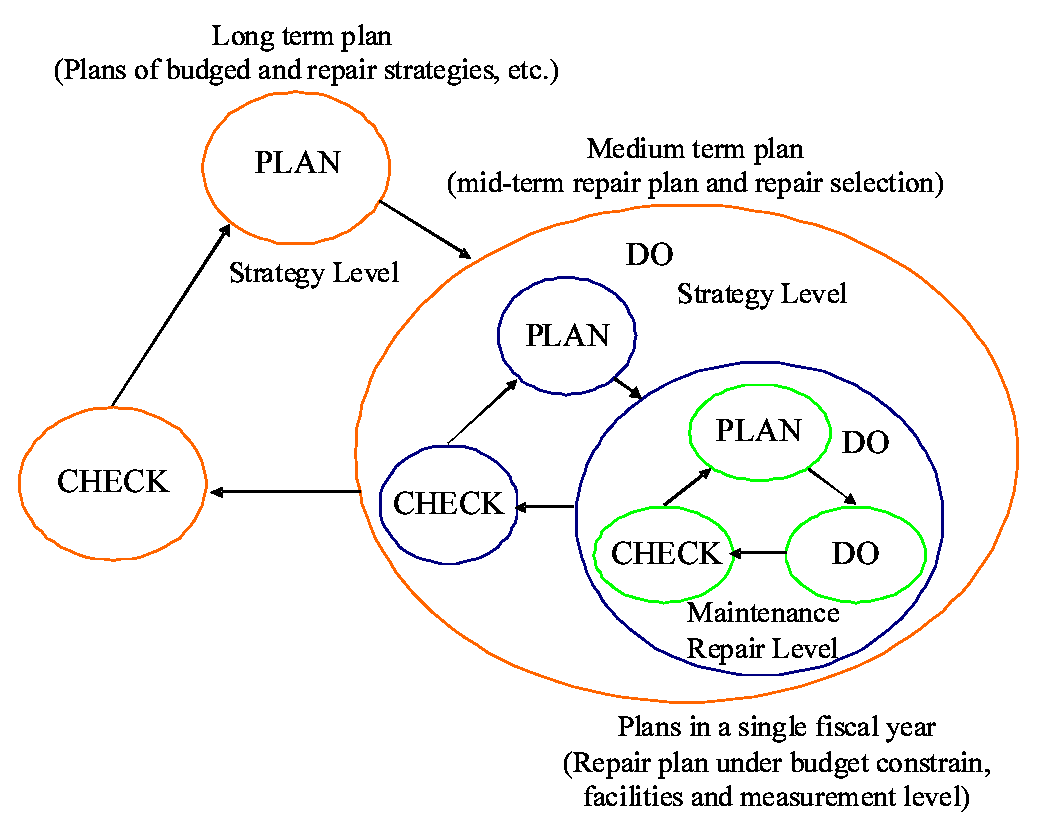
\includegraphics[scale=0.5]{fig21} 
\end{center}
\caption{Hierarchical Management Cycle.}
\label{fig21} 
\end{figure}

Management at top strategic level is understood as management of infrastructure network. The entire network is an integration or link of many infrastructure facilities. The objectives of management at network level are to define the service level for each group of infrastructure facility. This is an essential task in order to ensure the satisfaction and safety demanding from society. If the service level falls into poor status, as a sequent, various negative impacts will occurred. For example, bearing capacity of bridge concrete slab must always be in the range of acceptance \footnote{The bearing capacity of slab must always-above safety level, which is designated in structural analysis}. Otherwise, a collapse would happen that may not only cause economical loss but also claims the loss of life in some extend.

Further to long-term plan, one of the important assignment is ``How to evaluate and allocate a proper budget quota for each type or group of infrastructure''. In fact, budget allocation must be rigorously estimated by means of life cycle cost evaluation technique, which, in return, depending largely on the selection of the target service level, maintenance, and repair strategy. In practice, it is often the case that a set of the best maintenance and repair strategies are recommended for long-term management. The integration of hazard model and life cycle cost analysis becomes a vital tool to establish a state of control, a set of the best maintenance and repairs, which turns out to be the inputs or indicators for planning of the later phases.

Asking for middle-term plan, under the circumstance that a clear guidelines and outputs of long-term plan already established, the objective is to setting up a execution plan, which lists up the maintenance and repair activities on respective infrastructure facilities according to the priorities and the exposing risks. The top listed activities are expected to execute on the infrastructures, which expose to high-risk levels, having fast deteriorations and playing important service roles. In order to propose an appropriate list of actions, a sound monitoring system and measurement shall be engaged.

Regarding the management and repair level, which is often carried out within a fiscal year, budget allocation becomes a critical factor. Given the amount of fixed money from government and the priority list of action decided for middle-term plan, a detailed work break down structure for actual execution will be issued. In essence, the specific maintenance and repair will be scheduled according to its priority level and in connection with operation time of facilities. It is important at this stage to thoughtfully examine and record the actual performance of facilities and further document its updated status into inventory system.

As can be further discussed from the Figure \ref{fig21}, at all three levels of management, quality of work must be assured. Therefore, the Deming cycle \cite{deming} (PLAN-DO-CHECK) plays a center role. Any negligent performance may consequently lead to failure of management objectives at all levels. At first, a regular CHECK by mean of monitoring and inspection shall be well established. Secondly, a feasible PLAN with list of actions must be defined. Finally, implementing DO according to specification and guidelines \footnote{Deming cycle is widely applied in quality management, especially in business and operation of industrial factories. The center role of the cycle is toward continuous improvement of quality. A widely used abbreviation of the cycle is PDCA, meaning Plan, Do, Check, and Acts}.
%%%%%%%%%%%%%%%%%
\subsection{The Role of Hazard Model}
\label{222}
As previously explained, one of the important role in the control process for maintenance of infrastructure facility is to preserve facilities in smooth service standing. As the deterioration progresses by time, it turns out to be the task for maintenance and renovation of facilities, to keep the performance indicators in acceptable ranges. In this situation, the state of control and deterioration influencing factors must be accurately measured. By inspection and monitoring, we are able to keep an eye on the actual performance indicators. However, management and maintenance are also further extended to cover the future allocation of resources. This is therefore; hazard should be in place for predicting the progress of degradation, and for evaluating prominent environment factors contributing to the process. In essence, it is true to state that hazard model is the core of any infrastructure management program. Up to present, abundant of researches have been extensively documented with increasing emphasis on the dynamic deterioration mechanism \cite{kagi,kobami,tutu2,ono,qi,saeki}.

With respect to strategic level of management, the role of hazard model is to assist the selection for the state of control, the best guidelines for construction, maintenance, and repair, etc through the life cycle cost analysis. However, the difficulties are often encountered due to the demand in smoothly controlling and managing at the same time for hundreds or thousands of infrastructure facilities. Simply because, each infrastructure facility exerts to different deterioration behaviors due to variation of operation time, environment conditions and working loads. This task can only be successfully done through a hazard model, which considers all that factors for defining an average trend of deterioration for entire system. In fact, this approach is statistical dynamic oriented process that its accuracy largely relies on the accurate level in inspection and monitoring.

%Statistical hazard model toward dynamic deterioration mechanism with its advantages thus becomes the best method to address the deterioration problem in infrastructure asset management study and practice both at project and network point of views. Efforts in estimating average deterioration process of large number of infrastructure facilities have been carried out by using the information data from inspections \cite{kaito2}. 
%
To date, most of the hazard models have employed probabilistic and statistical approach, whereby, the state of control for infrastructure component is designated in discrete numbering range. The deterioration of infrastructure facility is simulated as transition pattern from one condition state to another condition state. However, the deterioration process bears its own uncertainty due to various endogenous and exogenous factors. To address this matter, it has been realized in recent years that the Markov chain model can be used to define the transition probability among the condition states. Interestingly, Markov chain model has been proved as the best applicable model in the sense of statistic and probability \cite{Takeyama,kenichi,Noriyuki}.

Further to Markov chain hazard model, much of the elaboration in estimating transition probability with inspection data is numerically estimated via maximum likelihood estimation technique. However, the challenges and difficulties somewhat belongs to how fit the assumption and presumption of model to be, and with respect to each type of infrastructure facility. Example of effort can be referred to Weibull hazard model for prediction the start of crack on pavement surface \cite{shin}, which typically discussed the issues of estimation under the missing of sufficient inspection data. The appealing challenge of presumption, on the other hand, opens the room for a large distribution of ongoing and future researches.

Keeping abreast of development trend in asset management, which tends to cope with the dynamic complexity of deterioration process and the trend of management, this research continues developing hazard model into several ankles, from a model which can apply generally on different type of infrastructure, to a specific model applied on a distinguish system. Special attention would be on presumption of parameters, embedded variables in hazard function and estimation approaches. In addition, empirical works shall be well addressed to link the theoretical part with practical implementation.
%%%%%%%%%%%%%%%%%%%%%
%\subsection{Future Perspectives of Asset Management}
%\label{223}
%Future fashion of infrastructure asset management system, as a matter of fact, depends much on the roles of the the system itself. In line with the overview of infrastructure asset management system, which already mentioned earlier with three levels of management, it is realized that the primary function of infrastructure asset management is resource management at all levels. Thus, if putting the future perspectives of infrastructure asset management on agenda, obvious to say, it is about the trails of how resources are going to be allocated. Thus, let us describe four trails of postulates which will justify the outlook of future asset management \footnote{The four trails are modified from \citet{bevpeter}}. Figure \ref{fig22} gives an idea of how the four trails link to corresponding aspects of management. 
%
%\begin{figure}[t]
%\begin{center}
%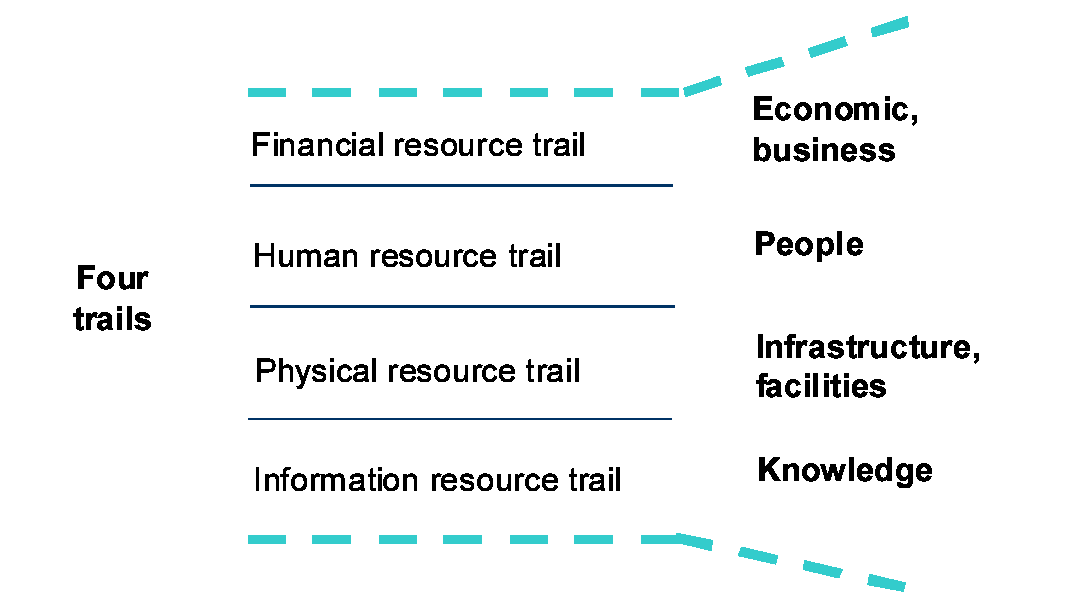
\includegraphics[scale=0.5]{fig22} 
%\end{center}
%\caption{Four generic trails of asset management to the future}
%\label{fig22} 
%\end{figure}
%
%\begin{itemize}
%\item{The financial trail will be the first to be discussed mainly due to the reasons that budget allocation for future construction work, which asset management accounts for a large share, is always of necessity. The question of how much, to where and when for maintenance and repair works should be tackle so as satisfying the equilibrium of resources in a long run. In addition, evaluation of infrastructure facilities in the view point of economic and finance eventually assist the formulation of best practices, best state of control, best maintenance and repair strategies for respective group of infrastructure. As the sequent, releasing heavy burdens of cost for society. The financial trails can also be further learned from the way that capital is mobilized among various stakeholders in society. For example, the participation of private section may change the traditional management fashion of public asset management in another form, which needs a carefully investigation so as service role of infrastructure can be sustained. A good solution in term of budget planning will hopefully enable future growth in sustainability.}
%
%\item{The human resource trail, as the second trail to be explored, could become the most revolutionary route to the future. A strong tendency has been realized that the working condition is projected to move in a dynamic and flexible form in the future with aids of advance technology, especially the ICT technology \cite{bevpeter}. Thus, the human resource deployment in the field of asset management should be well responded to ``place-flexibility'' and ``time flexibility'', probably towards a form of logistics management. In another word, the human resource logistic will need to become accountable for operational capacity, contingency provision, operational performance and operational effectiveness.}
%
%\item{Among the four trails, the physical resource trail exerts to be the most predicable trail to the future. This trail deals with the development of hazard model, characteristic factors influencing the performance of infrastructure facilities, measurement technology coping with ever changing environmental responses, etc. Especially, high intension on development of hazard model may be on trying to minimize the vulnerable exposing risks from nature such as: earthquake, climate change, flooding, land subsidence and raising of sea level so on and so forth.}
%
%\item{The last but possibly not least trail is information resource trail. In asset management, information resource firstly can be understood as results of inspection and monitoring. However, it can be extended to cover a wide range of knowledge concerning all facets of infrastructure management. In fact, the information trail covers an extremely wide territory, the herein mentioned just only belongs to a small part of it. Fundamentally, there are three main origins on which to build; knowledge of infrastructure itself, general management knowledge, and knowledge of design and maintenance in infrastructure system. In a nutshell of view, the first origin can be referred to monitoring activity, on which, performance indexes of infrastructure must be accurately stored in a systematic inventory system. This type of information shall be designed in the way to province the convenience to deterioration analysis and updating. The second origin refers again to the continuous management cycle described in Figure. \ref{fig21}, which would become a backbone concept in future  proactive management. The third origin can somehow regards as being undeveloped. However, a conclude point here is, the future development of asset management would turns to be in form of ``ASSET MATRIX'' involving learning capacity as a result of information or knowledge development.}
%
%\end{itemize}
%%%%%%%
\subsection{Characteristics of Monitoring Data}
\label{224}
Moving toward management approach with statistical and probabilistic deterioration model in the core, asset management practices must express collected information from monitoring and inspection in its front line. Indeed, the historical information is available, the better simulation of deterioration process become. In traditional hazard analysis with model of only binary mode, which is often seen in facility management (where condition state of facility is just simply GOOD or FAILURE), monitoring and inspection would not exercise much troubles because the condition state of facility can be captured visually.

In addition, the list of maintenance and repair is not numerous \cite{aoki2}. However, the working status or condition state of infrastructure facility like bridge, road, tunnel, etc are not just binary expression but often in a wide range of discrete numbers. Depending on the availability of technology in measurement, maintenance, and repair, the range of condition state may vary differently. In this scenario, we can only carry out the inspections following a regular period, likely two years for pavement system. In between of the inspections, condition state of infrastructure is impossible to be revealed. This issues lead to development of probabilistic study, which employs the Markov chain theory. However, the points shall be addressed here is, the requirement for monitoring and inspection extends to be among one of the most important task in infrastructure asset management.

Inspection and monitoring at present time and in the coming years are continuously improved, thanks to rapid development and innovation in technology. The condition state of infrastructure facility will be measured with more and more accuracy, and in the fast moving manner. For example, in pavement management system, nowadays, high-speed inspection care equipped with high-resolution camera and build-in electronic devices can rapidly transmit various forms of deterioration into inventory system and connecting with deterioration hazard model. However, in practice, monitoring and inspection have been examined in relatively low attention. The gathered information is often exposed to be in incompatible form that results in time consuming for verification and analysis. Thus, greater effort shall be imposed on creating a systemic monitoring and inspection procedure for respective type of infrastructure.

Further to issue in monitoring data, it has been worldwide recognizable that lack of data,  measurement errors, and bias are the major problems that push inaccurate outcome of hazard model. Condition state of infrastructure facility should be monitored and recorded throughout its service life. Information should cover all necessary indexes, from structural characteristic to environment imposing factors. This is, in fact, a critical issue since most of assumption and presumption for hazard model are based on the flow of inspection data. For example, Weibull hazard model can simulate the failure time and take the historical operation time into estimation \cite{aokia}. Whilst, Poisson deterioration model focus on the frequency of break happened on the infrastructure facility. 

More about the measurement errors and bias in monitoring, reasons could possibly due to errors or malfunctions of monitoring and measuring devices as well as human mistakes. This kind of problem is among the most fundamental troubles. And thus, beside a ready data filtering and verification, a need to further develop a hazard model which consider the measurement errors and bias would bring in a significant improvement in the field \cite{18}.
\section{Deterioration Hazard Model}
\label{23}
\subsection{Deterioration Process and Rating Index}
\label{231}
In order to analyze and forecast the deterioration of infrastructure components, it is necessary to accumulate time series data on the condition states of the components. The historical deterioration process of an infrastructure component is described in Figure \ref{fig23}. This figure shows the deterioration progress of a component that has not been repaired. In reality, there exists uncertainty in the deterioration progress of the component, and moreover, the condition state at each point in the time axis is restricted by the time, at which, visual inspection is carried out. 

In this figure, $\tau$ represents real calendar time (the expression ``time'' will be used instead throughout this paper). The deterioration of the infrastructure starts immediately after it is opened to the public at time $\tau_0$. The condition state of a component is expressed by a rank $J$ representing a state variable $i~(i=1,\cdots,J)$. For a component in the good or new situation, its condition state is given as $i=1$, and increasing of condition state $i$ describes progressing deterioration. A value of $i=J$ indicates that a component has reached its service limit. In Figure \ref{fig23}, for each discrete time $\tau_i~(i=1,\cdots,J-1)$ on the time-axis, the corresponding condition state has increased from $i$ to $i+1$. Hereinafter $\tau_i$ is referred to the time a transition from a condition state $i$ to $i+1$ occurs.

\begin{figure}[t]
\begin{center}
\includegraphics[scale=0.5]{fig23} 
\end{center}
\footnotesize Note) In this example, the deterioration process of a infrastructure component if expressed in terms of calendar time $\tau_1, \tau_2,...,\tau_i$, and condition state of the section is increased in unitary units.
\caption{Transition Time of Condition State.}
\label{fig23} 
\end{figure}
%%
%
Information regarding the deterioration process of an infrastructure can be acquired through periodical visual inspections. However, information on the condition state based on continuous visual inspection is difficult to obtain. In this case, the initial inspections is carried out at times $\tau_A$ on the time-axis. It is supposed that at time $\tau_A$ the condition state observed by inspection is $i~(i=1,\cdots,J-1)$. The deterioration progress in future times is uncertain. Among the infinite set of possible scenarios describing the deterioration process only one path is finally realized. 

Figure \ref{fig24} shows four possible sample paths. Path 1 shows no transition in the condition state $1$ from initial time $\tau_0$ to first inspection time $\tau_A$. In paths 2 and 3, condition state has advanced to one upper state condition at the calendar times $\tau_1^2$ and $\tau_1^3$ respectively. The condition state of these two paths observed at time $\tau_A$ become $2$. In a periodical inspection scheme, the point times $\tau_1^2$ and $\tau_1^3$ in which the condition state has changed from $1$ to $2$ are not determined. In addition, path 4 shows transitions in the condition state at times $\tau_i^4$ and $\tau_{i+1}^4$ during the inspection interval. The condition state observed at time $\tau_A$ becomes $3$. That is, in spite of the transitions in the condition state are observable at the time of periodical inspection, it is not possible to obtain information about the times in which those transitions occur.

Figure \ref{fig25} further describes the deterioration process inferring the inspection approach and how the condition state is assumed. In this figure, it is assumed that the condition state at the calendar time $\tau_{i-1}$ has changed from $i-1$ to $i$. The calendar time $\tau_{i-1}$ is assumed to be equivalent to $y_i=0$. The time represented by the sample time-axis is referred from now on as a ``time point'', and differs from ``time'' on the calendar time axis. The times $\tau_A$ and $\tau_B$ correspond to the time points $y_A$ and $y_B$ on the sample axis. It can be seen that $y_A=\tau_A-\tau_{i-1}$, $y_B=\tau_B-\tau_{i-1}$. 

Information on the condition state $i$ at the beginning of the calendar time $\tau_{i-1}$ cannot be obtained in a periodical inspection scheme. Therefore, time points $y_A$ and $y_B$ on the sample time-axis cannot be correctly obtained either. For convenience of description, it is assumed that the information at the time a point is known in order to develop the model, despite this assumption is not necessarily essential. The following paragraph discusses that even without information at time points $y_A$ and $y_B$ an exponential hazard model can be estimated.
\begin{figure}[t]
\begin{center}
\includegraphics[scale=0.5]{fig24} 
\end{center}
\footnotesize Note) In this example, the deterioration process of an infrastructure component is expressed in terms of four different sample paths. In paths 2 and 3 the condition state has advanced to one upper state condition at the calendar times $\tau_1^2$ and $\tau_1^3$ respectively. In path 4, the condition state has increased one state at each time $\tau_1^4$ and $\tau_{2}^4$. However, in the case of a periodical inspection carried out at times $\tau_A$ the condition state at any point in time between inspections cannot be observed.
\caption{Transition Pattern of Condition State.}
\label{fig24} 
\end{figure}

In the case the condition state of a infrastructure component at time $\tau_{i}$ (time point $y_C$) is assumed to change from $i$ to $i+1$, the period length in which the condition state has remained at $i$ (referred as the life expectancy of a condition state $i$) is represented by $\zeta_i=\tau_{i}-\tau_{i-1}=y_C$. The life expectancy of a condition state $i$ is assumed to be a stochastic variable $\zeta_i$ with probability density function $f_i(\zeta_i)$ and distribution function $F_i(\zeta_i)$. Random variable $\zeta_i$ is defined in the domain $[0,\infty]$. The distribution function is defined as
\begin{eqnarray}
&& F_i(y_i)=\int_0^{y_i}f_i(\zeta_i)d\zeta_i. \label{func21}
\end{eqnarray}
\begin{figure}[t]
\begin{center}
\includegraphics[scale=0.5]{fig25} 
\end{center}
\footnotesize Note) In the case the condition state changes from $i-1$ to $i$ at the calendar time $\tau_{i-1}$ the inspections carried out at times $\tau_A$ and $\tau_B$ will also correspond to the points in time $y_A$ and $y_B$ when using $\tau_{i-1}$ as the time origin. The figure shows a sample deterioration path in which the condition state has advanced in one unit to $y_c$ in the interval time $\tau_{i-1}-y_C$. However, observations at time $\tau_{i-1}$ are not possible in a periodical inspection scheme, so there is no way to obtain observation at $y_A$, $y_B$ and $y_C$. Nevertheless, it is possible to use the information contained in $z=y_C-y_A \in [0,Z]$.
\caption{Model of Deterioration Process.}
\label{fig25} 
\end{figure}

The distribution function $F_i(y_i)$ represents the cumulative probability of the transition in the condition state from $i$ to $i+1$. Condition state $i$ is assumed to be observed at initial time $y_i=0$(time $\tau_A$). The time interval measured along the sample time-axis until the time point $y_i$ is $\tau_{i-1}+y_i$. Therefore, using the cumulative probability $F_i(y_i)$, the probability $\tilde{F}_i(y_i)$ of a transition in the condition state $i$ during the time points interval $y_i=0$ to $y_i\in [0,\infty]$ is defined by $\tilde{F}_i(y_i)$:
\begin{eqnarray}
&& \mbox{Prob}\{\zeta_i \geq y_i\}= \tilde{F}_i(y_i) = 1 -  F_i(y_i). \label{funcbF}
\end{eqnarray}
The conditional probability that the condition state of a component at time $y_i$ advances from $i$ to $i+1$ during the time interval $[y_i,y_i+\Delta y_i]$ is defined as
\begin{eqnarray}
&& \lambda_i(y_i) \Delta y_i = \frac{f_i(y_i)\Delta y_i}{\tilde{F}_i(y_i)}  \label{riskbF},
\end{eqnarray}
where the probability density $\lambda_i(y_i)$ is referred as the hazard function.
%%%%%%%%%%%%%%
\subsection{Markov Transition Probability}
\label{232}
The transition process among the condition states of an infrastructure component is uncertain. Therefore, future condition states cannot be forecasted deterministically. In this situation, Markov transition probability is employed to represent the uncertain transition pattern of the condition states during two time points. Markov transition probabilities can be defined for arbitrary time intervals. 

For simplification, Markov transition probabilities can be defined and used to forecast the deterioration of a infrastructure component based on the information from periodical inspection scheme shown in Figure \ref{fig25}. The observed condition state of the component at time $\tau_A$ is expressed by using the state variable $h(\tau_A) $. If the condition state observed at time $\tau_A$ is $i$, then the state variable $h(\tau_A)=i$. A Markov transition probability, given a condition state $h(\tau_A) =i$ observed at time $\tau_A$, defines the probability that the condition state at a future time ($\tau_B$ for example) will change to $h(\tau_B) =j$:
\begin{eqnarray}
&& \mbox{Prob}[h(\tau_B)=j|h(\tau_A)=i]=\pi_{ij}.\label{pro}
\end{eqnarray}
The Markov transition probability matrix can be defined and rearranged by using the transition probabilities between each pair of condition states $(i,j)$ as
\begin{eqnarray}
&& {\bf \Pi}=\left(
\begin{array}{ccc}
\pi_{11} & \cdots & \pi_{1J} \\
\vdots & \ddots & \vdots \\
0 & \cdots & \pi_{JJ}
\end{array}
\right). 
\end{eqnarray}
The Markov transition probability (\ref{pro}) shows the transition probability between the condition states at two given times $\tau_A$ and $\tau_B$, therefore, it is straightforward that the values of a transition probability will differ for different time intervals. Since deterioration continues as long as no repair is carried out $\pi_{ij}=0~(i>j)$. From the definition of transition probability $\sum^{J}_{j=1}\pi_{ij}=1$. Following conditions must be satisfied:
\begin{eqnarray}
\left.
\begin{array}{l}
\pi_{ij}\geq 0 \\
\pi_{ij}=0 \,\,~(\,\mbox{when} \,\,\, i>j) \\
\sum_{j=1}^J \pi_{ij}=1 \\
\end{array}
\right\}.\label{suii}
\end{eqnarray}
The worse level of deterioration is expressed by the condition state $J$, which remains as an absorbing state in the Markov chain as long as no repair is carried out. In this case $\pi_{JJ}=1$.

Markov transition probabilities are defined independently from the deterioration history. As shown in Figure \ref{fig25}, the condition state at the inspection time $\tau_A$ is $i$, however, the time, at which, condition state changed from $i-1$ to $i$ is unobservable. In a Markov chain model, it is assumed that the transition probability between the inspection times $\tau_A$ and $\tau_B$ is only dependent on the condition state at time $\tau_A$. 

The Markov chain model is operative and widely applied in management of infrastructure system. Particularly, at management of network level, Markov chain model is used to define the average transition probability of the entire system, or a group of infrastructure components given two periodical inspection data.
%%%%%%%%%%%%%%%%%%%%%%%%
\subsection{Exponential Hazard Model}
\label{233}
%%%%%%%%%%%%%%%%%%%%%%%%%%%%%%%%%%
In this section, it is assumed that the deterioration of a infrastructure component satisfies Markov property, and the hazard function is independent of the time $y_i$ on the time-axis. That is, for a fixed value of $\theta_i>0$, we have
\begin{eqnarray}
&& \lambda_i(y_i)=\theta_i \hspace{2mm}. \label{hazard}
\end{eqnarray}
By using the hazard function (\ref{hazard}), it is possible to represent a deterioration process of a infrastructure component that satisfies the Markov property (Independence from the past history). In addition, it is assumed that $\theta_i\neq \theta_j~(i \neq j)$. By differentiating both sides of equation (\ref{funcbF}) with respect to $y_i$,
\begin{eqnarray}
&& \frac{d\tilde{F}_i(y_i)}{dy_i}=-f_i(y_i).\label{op}
\end{eqnarray}
Equation (\ref{riskbF}) then becomes
\begin{eqnarray}
&& \lambda_i(y_i) = \frac{f_i(y_i)}{\tilde{F}_i(y_i)} =-\frac{\frac{d\tilde{F}_i(y_i)}{dy_i}}{\tilde{F}(y_i)} 
= \frac{d}{dy_i}\left( - \log \tilde{F}_i(y_i) \right).\label{opi}
\end{eqnarray}
Considering that $\tilde{F}_i(0)=1-F_i(0)=1$, and by integrating equation (\ref{opi}), we come up with
\begin{eqnarray}
&& \hspace{-9mm} \int_{0}^{y_i} \lambda_i(u)du = \big[-\log \tilde{F}_i(u)\big]_{0}^{y_i} = -\log \tilde{F}_i(y_i).
\end{eqnarray}
Using the hazard function $\lambda_i(y_i)=\theta_i$, the probability $\tilde{F}_i(y_i)$ that the life expectancy of the condition state $i$ becoming longer than $y_i$ is expressed by
\begin{eqnarray}
&& \tilde{F}_i(y_i) = \exp \left[ - \int_{0}^{y_i}\lambda_i(u)du \right] 
 = \exp (-\theta_i y_i). \label{prop-bFla}
\end{eqnarray}
Equation (\ref{prop-bFla}) is exponential form of hazard model. According to equation (\ref{op}), the probability density function $f_i(\zeta_i)$ of the life expectancy of the condition state $i$ is
\begin{eqnarray}
&& f_i(\zeta_i)=\theta_i \exp(-\theta_i \zeta_i).\label{kikan}
\end{eqnarray}
By then, considering that the condition state has changed to $i$ at the time  $\tau_{i-1}$, and remains constant until the inspection time $\tau_A$. Obvious to say, the condition state observed at inspection time $\tau_A$ is $i$. In term of duration, condition state $i$ has actually stayed in the period $y_A$. The probability, to which the condition state $i$ keeps remaining in a subsequent time $z_i~(\geq 0)$ measured after the duration $y_A$, is then defined:
\begin{eqnarray}
&& \tilde{F}_i(y_A+z_i|\zeta_i \geq y_A) 
 = \mbox{Prob} \{\zeta_i \geq y_A+z_i | \zeta_i \geq y_A\}. \label{eq213}
\end{eqnarray}
Dividing both sides of equation (\ref{eq213}) by the probability $\tilde{F}_i(y_i)$ described in equation (\ref{funcbF}) results in
\begin{eqnarray}
&& \frac{\mbox{Prob} \{\zeta_i \geq y_A+z_i\}}{ \mbox{Prob}\{\zeta_i \geq y_A\}} = \frac{\tilde{F}_i(y_A+z_i)}{\tilde{F}_i(y_A)}. \label{eq214}
\end{eqnarray}
With reference to equation (\ref{prop-bFla}), the right side of equation (\ref{eq214}) becomes:
\begin{eqnarray}
&& \frac{\tilde{F}_i(y_A+z_i)}{\tilde{F}_i(y_A)}= \frac{\exp \{-\theta_i (y_A+z_i)\}}{\exp( - \theta_i y_A)} 
 =\exp (-\theta_i z_i). \label{eq215}
\end{eqnarray}
Based on this conditional rule, we can define the probability, to which, the condition state $i$ observed at time $\tau_A$ continues to be observed at subsequent inspection time $y_B=y_A+Z$ is analogous to equation (\ref{eq215}):
\begin{eqnarray}
&& \hspace{-3mm} \mbox{Prob}[h(y_B)=i|h(y_A)=i]=\exp(-\theta_i Z), \label{pro1},
\end{eqnarray}
where $Z$ expresses the interval between two inspection times. The probability $\mbox{Prob}[h(y_B)=i|h(y_A)=i]$ is nothing but the Markov transition probability $\pi_{ii} $. Obviously, if the exponential hazard function is employed, the transition probability $\pi_{ii} $ is dependent only on the hazard rate $\theta_i$ and the inspection interval $Z$.
%Even more, without using deterministic information on the time points $y_A$ and $y_B$, it is still possible to estimate transition probabilities.
%%%%%%%%%%%%%%%%%%%%%%%%%%55
\subsection{Weibull Hazard Model}
\label{234}
In reality, the data concerning deterioration of infrastructure facilities are not only condition state but also their embedded characteristics. This information can be observed from inspections. However, in actual practices, the inspection intervals of different infrastructure, components do not possess the same duration. In this respect, Markov chain model using only two recent inspection data might not reflect overall performance. Weibull hazard function can capture the historical performance is thus beneficial in this circumstance. 

The assumption of deterioration can be referred to Figure \ref{fig26}. In this figure, condition state starts to change from $i-1$ to $i$ at time $\tau_{i-1}$. $y_i$ is elapsed time or duration of stay in condition state $i$. The duration $y_A$ is estimated by $y_A = \tau_A - \tau_{i-1}$ and understood as the elapsed time between calendar time $\tau_{i-1}$ and $\tau_A$.

\begin{figure}[t]
\begin{center}
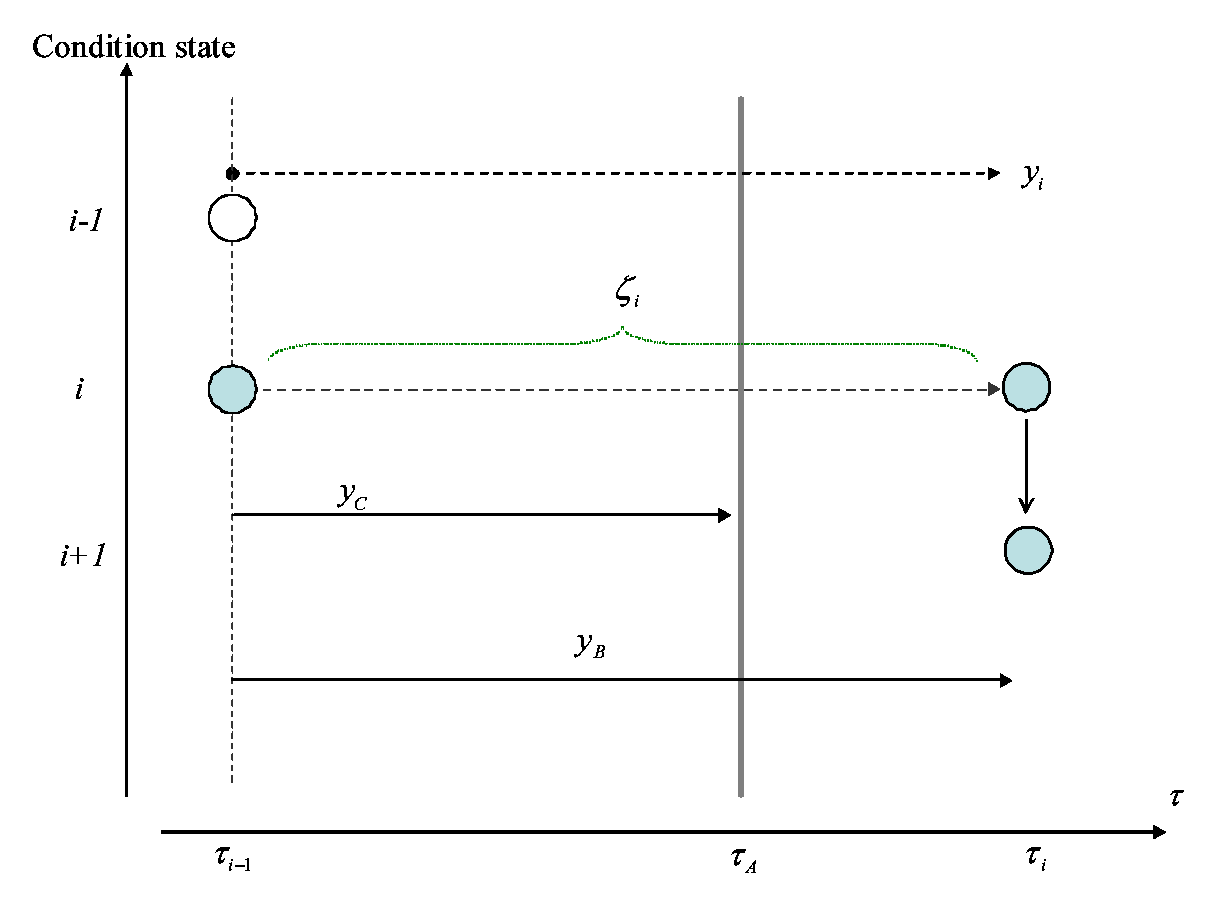
\includegraphics[scale=0.5]{fig26} 
\end{center}
\footnotesize Note) Condition state changes from $i-1$ to $i$ at calendar time $\tau_{i-1}$, which refers as starting point of deterioration process. The inspection is carried out at time $\tau_A$ and at which we have corresponding time length $y_A$ counted from $\tau_{i-1}$. The condition state continues to occupy length $y_B$ in its deterioration path. However, at time $\tau_{i-1}$, there is no observation. In the sequel, the exact time length $y_A$ and $y_B$ on the time axis can not be determined.
\caption{Condition State and Inspection Interval.}
\label{fig26} 
\end{figure}
%%%
From equations (\ref{func21}-\ref{riskbF}), applying similar mathematical approach like in equations (\ref{op}-\ref{pro1}), in the form of Weibull distribution, hazard function $\lambda_i$, survival probability $\tilde{F} _ i(y_i)$ and probability density function $f_i(\zeta_i)$ can be expressed: 
\begin{eqnarray}
&& \lambda_i(y_i)= \theta_i \alpha_{i} y_i^{\alpha_{i}-1}, \label{hazardw}\\
&& \tilde{F}_i(y_i) = \exp (-\theta_i y_i^{\alpha_{i}}), \label{prop-bFlaw}\\
&& f_i(\zeta_i)=\theta_i \alpha_{i} \zeta^{\alpha_{i}-1}_i\exp(-\theta_i \zeta^{\alpha_{i}}_i).\label{kikanw}
\end{eqnarray}
%%%%%%%%%%%%%
\section{Deterioration Hazard Model Estimation Method}
\label{24}
\subsection{Exponential hazard model}
\label{241}
\subsubsection{Defining Markov transition probabilities}
\label{2411}
This section continues the formation of transition probability earlier explained in section \ref{232} and section \ref{233} for general case.

Let us discuss the formulation of model in the case condition state $i$ advancing in only one-step, to condition state $i+1$ in the inspection interval from $\tau_A$ to $\tau_B$. At first, it is assumed that condition state $i$ remains during duration $y_A$ and in subsequent increment of time $s_i=y_A+z_i, (z_i\in [0,Z])$. Secondly, condition state $i$ changes into $i+1$ at $y_A+z_i$. Thirdly, condition state $i+1$ keep unchanging during the interval $[y_A+z_i$, $y_B]$.

Although the exact time, at which the condition state transits from $i$ to $i+1$ can not be traced by periodical inspection, it can be temporarily assumed that the transition occurs at the time point $(y_A+\bar{z}_i) \in [y_A,y_B]$. Given the condition state $i$ staying during $y_A$ and remains until the time $y_A+\bar{z}_i$, the conditional probability density, to which condition state $i+1$ being observed at $y_A+\bar{z}_i$ can be defined:
\begin{eqnarray}
&& \hspace{-8mm} g_i(\bar{z}_i|\zeta_i \geq y_A)=\frac{f_i(\bar{z}_i+y_A)}{\tilde{F}_i(y_A)} 
 =\frac{\theta_i \exp\{-\theta_i (\bar{z}_i+y_A)\}}{\exp(-\theta_i y_A)}
=\theta_i \exp(-\theta_i \bar{z}_i).
\end{eqnarray}
Satisfying the above condition, the conditional probability density that the condition state $i+1$ being observed at the inspection time $y_B$ becomes:
\begin{eqnarray}
&& \hspace{-3mm} q_{i+1}(\bar{z}_i|\zeta_i\geq y_A) 
 = g_i(\bar{z}_i|\zeta_i \geq y_A) \cdot \tilde{F}_{i+1}(y_B-\bar{z}_i-y_A) \nonumber\\
&& = \theta_i \exp(-\theta_i \bar{z}_i) \exp\{-\theta_{i+1}(Z-\bar{z}_i)\} \nonumber\\
&& = \theta_i \exp(-\theta_{i+1}Z)\exp\{-(\theta_i-\theta_{i+1})\bar{z}_i\}.
\end{eqnarray}
It is noticed that $\bar{s}_i=y_A+\bar{z}_i$ is assumed as fixed value. However, the elapsed time $\zeta_i$ of a condition state $i$ is truly a stochastic variable, thus,  $\bar{z}_i$ may change in range $[0, Z] $. The Markov transition probability that the condition state change from $i$ to $i+1$ during the time points $y_A$ and $y_B$ is then defined by the law of integration:
\begin{eqnarray}
&& \hspace{-5mm} \pi_{ii+1}=\mbox{Prob}[h(y_B)=i+1|h(y_A)=i] 
 =\int_{0}^{Z} q_{i+1}(z_i|\zeta_i\geq y_A)dz_i \nonumber \\
&& \hspace{-3mm} =\int_0^{Z} \theta_i \exp(-\theta_{i+1}Z)\exp\{-(\theta_i-\theta_{i+1})z_i\}dz_i \nonumber \\
&& \hspace{-3mm} = \frac{\theta_i}{\theta_{i}-\theta_{i+1}}\{-\exp(-\theta_{i}Z)+\exp(-\theta_{i+1}Z)\},\label{iik}
\end{eqnarray}
where $\pi_{ii+1}>0$ is indifferent to the relative size between $\theta_i$ and $\theta_j$. The assumption $\theta_i\neq \theta_{i+1}$ implies $1>\pi_{ii+1}$. As these characteristics are trivial in the derivation process of equation (\ref{iik}), the verification is omitted. 

Moving to general case, when in the next inspection, condition state $j(j\geq i +2)$ is observed. The distribution function and the probability density function concerning the duration condition state $j$ actually stays in can be assumed as $F_j(y_j) $ and $f_j(y_j)$. The hazard function applying on the condition state $j$ is denoted by $\lambda_j(y_j) =\theta_j$. 

The process, where by happening the transition of condition state from $i$ to $i+1$ during interval $[y_A,y_B]$ can be perceived as follows. At first, the condition state $i$ remains during the elapsed time $y_A$ and in a subsequent time $\bar{s}_i=y_A+\bar{z}_i \in [y_A,y_B]$. Secondly, exactly at time $\bar{s}_i=y_A+\bar{z}_i$, condition state $i$ changes into $i+1$. Thirdly, condition state $i+1$ remains in the duration $[\bar{s}_i=y_A+\bar{z}_i, \bar{s}_{i+1}=\bar{s}_{i}+\bar{z}_{i+1}~(\leq y_B)]$ before turning to condition state $i+2$ at $\bar{s}_{i+1}=\bar{s}_{i}+\bar{z}_{i+1}$. Fourthly, after repeating the same transition process, condition state happens to change into $j$ at time $\bar{s}_{j-1}~(\leq y_B)$, and keep unchanging until inspection time $y_B$. If the entire process of transition is considered, a simultaneously conditional probability density function can be defined as follow:
\begin{eqnarray}
&& q_{j}(\bar{z}_i,\bar{z}_{i+1},\cdots,\bar{z}_{j-1}|\zeta_i\geq y_A) \nonumber \\
&& = g_i(\bar{z}_i|\zeta_i \geq y_A) \prod_{m=i+1}^{j-1} f_{m}(\bar{z}_m) \tilde{F}_{j}\left(Z-\sum_{m=i}^{j-1} \bar{z}_m\right)
\nonumber\\
&& = \prod_{m=i}^{j-1}\theta_m\cdot \exp\left\{- \sum_{m=i}^{j-1} \theta_m \bar{z}_m -\theta_{j}(Z-\sum_{m=i}^{j-1} \bar{z}_m)\right\}\nonumber \\
&& = \prod_{m=i}^{j-1}\theta_m \cdot \exp\left\{-\theta_j Z - \sum_{m=i}^{j-1} (\theta_m-\theta_{j})\bar{z}_m\right\},
\end{eqnarray}
where $\bar{z}_i,\cdots,\bar{z}_{j-1}$ are regarded as fixed values. However, the elapsed time $\zeta_i$ of condition states $i~(i=1,\cdots,J-1)$ is a stochastic variable, the values of $z_i\geq 0,\cdots,z_{j-1}\geq 0$ are variable, which subject to satisfy the following condition:
\begin{eqnarray}
&& 0\leq z_i+z_{i+1}+\cdots+z_{j-1}\leq Z.
\end{eqnarray}
As the sequent, for continuous observed time, the Markov transition probabilities $\pi_{ij}$ is conditional probability and being described in following equation:
\begin{eqnarray}
&& \hspace{-10mm} \pi_{ij}=\mbox{Prob}[h(y_B)=j|h(y_A)=i] 
 =\int_{0}^{Z}\int_0^{Z-z_i} \cdots \int_{0}^{Z-\sum_{m=i}^{j-2}z_{m}}\nonumber \\
&& \hspace{-5mm} q_{j}(z_i,\cdots,z_{j-1}|\zeta_i\geq y_A)dz_i\cdots dz_{j-1} \nonumber \\
&& \hspace{-10mm} =\sum_{k=i}^{j}\prod_{m=i}^{k-1}\frac{\theta_m}{\theta_{m}-\theta_{k}}\prod_{m=k}^{j-1}\frac{\theta_m}{\theta_{m+1}-\theta_{k}}\exp(- \theta_{k} Z). \label{dousyutu}
\end{eqnarray}
Details of description for getting into equation (\ref{dousyutu}) is given in the paper of \citet{kobayashitsuda}. For convenient reading, general forms of Markov transition probabilities are given in the following equations:
\begin{manyeqns}
&& \pi_{ii}=\exp(-\theta_i Z), \label{p1} \\
&& \pi_{ii+1}= \frac{\theta_i}{\theta_{i}-\theta_{i+1}}\{-\exp(-\theta_{i}Z)+\exp(-\theta_{i+1}Z)\}, \\
&& \pi_{ij}= \sum_{k=i}^{j}\prod_{m=i}^{k-1}\frac{\theta_m}{\theta_{m}-\theta_{k}}\prod_{m=k}^{j-1}\frac{\theta_m}{\theta_{m+1}-\theta_{k}}\exp(- \theta_{k} Z) \label{hazardpiij}, \\
&& \pi_{iJ}=1-\sum_{j=i}^{J-1}\pi_{ij}, \label{pj}\\
&& \hspace{5mm} (i=1,\cdots,J-1) \hspace{5mm} (j=i,\cdots,J). \nonumber
\end{manyeqns}
%%%%
\subsubsection{Time adjustment of Markov transition probability}
\label{2412}
%%%%
Markov transition probabilities depend on the inspection interval $Z$ as can be revealed from equations (\ref{p1}) - (\ref{pj}). In cardinal matrix form, we can further expressed the time interval depend of Markov transition probability:
\begin{eqnarray}
&& \mbox{\boldmath$\Pi$}(Z)=\left(
\begin{array}{ccc}
\pi_{11}(Z) & \cdots & \pi_{1J}(Z) \\
\vdots & \ddots & \vdots \\
0 & \cdots  & \pi_{JJ}(Z)
\end{array}
\right).
\end{eqnarray}
Inspections are scheduled in a regular based time with integer number $n$. If two inspection interval $Z$ and $nZ$ are considered, the two Markov transition probability matrix $\mbox{\boldmath$\Pi$} (Z) $ and $\mbox{\boldmath$\Pi$} (nZ) $ can also be used to express the dependency on inspection interval. Based on the law of matrix multiplication, the relation between $\mbox{\boldmath$\Pi$} (Z) $ and $\mbox{\boldmath$\Pi$} (nZ) $ is clearly defined:
\begin{eqnarray}
&& \mbox{\boldmath$\Pi$}(nZ)=\left\{\mbox{\boldmath$\Pi$}(Z)\right\}^n .\label{seigou}
\end{eqnarray}
Equation (\ref{seigou}) expresses the time adjustment condition of the Markov transition probability matrix. If $n$ becomes very big number, a stationary state of transition probabilities will be obtained. It is concluded here that with respect to different time interval $Z$, we can adjust the properties of Markov transition probability to reflect the actual inspection schedule in practices.
%%%%%%%%%%
\subsubsection{Estimation of Markov Transition Probability}
\label{2413}
\textit{(a) Contents of periodical inspection data}

Suppose periodical inspection data on the same kind of $K$ infrastructure components is available. An inspection sample $k(k= 1, \cdots, K) $ describes two continuous periodical inspections carried out at times $\tau_A^k$ and $\tau_B^k$ and the respective condition states ratings $h(\tau_A^k)$ and $h(\tau_B^k)$ measured at those times. Differences in the inspection intervals of the samples are inconvenient. Based on the above inspection data, the inspection interval of a sample $k$ is defined as $Z^k=\tau_B^k-\tau_A^k$. In addition a dummy variable $\delta_{ij}^k~(i,j=1,\cdots,J; k=1,\cdots,K)$ based on the deterioration progress patterns between two inspections times is defined as
\begin{eqnarray}
&& \hspace{-8mm} \delta_{ij}^k=\left\{
\begin{array}{ll}
1 & \mbox{when} \;\,h(\tau_A^k)=i \;\,\mbox{and}\;\, h(\tau_B^k)=j\\
0 & \mbox{otherwise}
\end{array}.
\right.
\end{eqnarray}
Furthermore, the structural characteristics and usage conditions that affect the deterioration of an infrastructure component are represented by the vector $\mbox{\boldmath$x$}^k=(x_1^k,\cdots,x_M^k)$. $x_m^k~(m=1,\cdots,M)$ represents the value of a characteristic variable $m$ observed in the sample data $k$. The information contained in the inspection sample data $k$ can be rearranged as $\Xi^k=(\delta_ {ij} ^k, Z^k, \mbox{\boldmath$x$}^k) $. On the other hand, the exponential hazard function of the deterioration process for a sample data $k(k= 1, \cdots, K) $ is 
\begin{eqnarray}
&& \lambda_i^k(y_i^k)=\theta_i^k ~(i=1,\cdots,J-1). \nonumber
\end{eqnarray}
It is noted here that the hazard rate for condition state $J$ is not defined because $J$ is absorbing condition state ($\pi_{JJ} =1$). The hazard rate $\theta_i^k~(i=1,\cdots,J-1;k=1,\cdots,K)$ characterizing the deterioration process is considered to change in relation to the vector $\mbox{\boldmath$x$}^k$ as follow: 
\begin{eqnarray}
&& \theta_i^k=\mbox{\boldmath$x$}^k\mbox{\boldmath$\beta$}_i^\prime ,\label{hazard1}
\end{eqnarray}
where $\mbox{\boldmath$\beta$}_i=(\beta_{i,1},\cdots,\beta_{i,M})$ is a row vector of unknown parameters $\beta_{i,m}~(m=1,\cdots,M)$ and the symbol $\prime$ indicates the vector is transposed. In order to obtain Markov transition probabilities, at first, the exponential hazard function $\lambda_i^k(y_i^k)=\theta_i^k$ is estimated based on the observed sampling information $\Xi^k~(k=1,\cdots,K)$. Secondly, Markov transition probabilities can be estimated based on the relation with hazard function. 

This methodology permits estimation for Markov transition probabilities of every individual infrastructure component. However, as a rule of thumb, it is better to estimate the average transition probability for the entire group of infrastructure instead of estimating for individual component. 

\textit{(b) Infrastructure management indicators}

Using exponential hazard model, we can define one of the important management indicator for infrastructure. The indicator is the remaining duration ($RMD_i$) of condition state $i$, which reflects how long condition state $i$ can survive given condition that it has been observed in previous inspection time. $RMD_i$ is actually analogous to survival function $\tilde{F}_i(y_i^k)$ in infinite domain \cite{lancaster90}:
\begin{eqnarray}
&& RMD_i^k= \int^{\infty}_{0}\tilde{F}_i(y_i^k)dy_i^k \hspace{1mm}.\label{17}
\end{eqnarray}
Based on equation (\ref{prop-bFla}), the remaining duration $RMD^k_i$ of component $k$ can be further defined in the exponential form:
\begin{eqnarray}
&& RMD_i^k= \int^{\infty}_{0}\exp (-\theta_i^k y_i^k) dy_i^k = \frac{1}{\theta_i^k} \hspace{1mm}.\label{rating}
\end{eqnarray}
Assuming the condition state after opening the infrastructure is $i$. The expected value $ET_j~(j=2,\cdots,J)$ referred as average life expectancy of condition state $j$, is thus a summation of all transition duration from every condition state $i$:
\begin{eqnarray}
&& ET_j=\sum_{i=1}^j \frac{1}{\lambda_i}\hspace{1mm}. \label{hy}
\end{eqnarray}
Rating $j~(j=1\cdots,J)$ and average relation of elapsed time $ET_j(\mbox{\boldmath$x$})$  are used to draw the expectation deterioration curve.
%%%%%%%%%%%%

\textit{(c) Estimation of the hazard model}

Information $\Xi^k=(\bar{\delta}_{ij}^k,\bar{Z}^k,\bar{\mbox{\boldmath$x$}}^k)$ can be acquired in relation to the inspection sample $k$, where the symbol $\bar{}$ indicates an actual measurement. The Markov transition probabilities can be expressed in terms of the hazard functions as described in equations (\ref{p1})-(\ref{pj}). The relationship between hazard rate $\theta_i^k~(i=1,\cdots,J-1;k=1,\cdots,K)$ and the characteristic variables $\bar{\mbox{\boldmath$x$}}^k$ is shown in equation (\ref{hazard1}). Moreover, the transition probability also depends on inspection interval $\bar{Z}^k$.

For clarity of presentation, the transition probability $\pi_{ij}$ is expressed as a function of the measured data $(\bar{Z}^k,\bar{\mbox{\boldmath$x$}}^k)$ obtained from visual inspection and the unknown parameters $\mbox{\boldmath$\beta$}_i$ as $\pi_{ij}(\bar{Z}^k,\bar{\mbox{\boldmath$x$}}^k:\mbox{\boldmath$\beta$}_i)$. If the deterioration progress of the infrastructure components in a sample $K$ are assumed to be mutually independent, the log-likelihood function expressing the simultaneous probability density of the deterioration transition pattern for all inspection samples is \cite{tobin,amemi}
\begin{eqnarray}
&& \hspace{-3mm} \ln[{\cal L}(\mbox{\boldmath$\beta$})] = \ln \left[\prod_{i=1}^{J-1} \prod_{j=i}^J\prod_{k=1}^{K} \left\{\pi_{ij}(\bar{Z}^k,\bar{\mbox{\boldmath$x$}}^k:\mbox{\boldmath$\beta$})\right\}^{\bar{\delta}_{ij}^k}\right]
\nonumber \\
&& \hspace{5mm} =\sum_{i=1}^{J-1} \sum_{j=i}^J\sum_{k=1}^K \bar{\delta}_{ij}^k \ln\left[
\pi_{ij}(\bar{Z}^k,\bar{\mbox{\boldmath$x$}}^k:\mbox{\boldmath$\beta$})\right] \hspace{1mm},
 \label{logbF}
\end{eqnarray}
where $\bar{\delta}_{ij}^k$, $\bar{Z}^k$ and  $\bar{\mbox{\boldmath$x$}}^k$ are all determined through inspections, and $\mbox{\boldmath$\beta$}_i~(i=1,\cdots,J-1)$ are parameters to be estimated. Estimations of the parameters $\mbox{\boldmath$\beta$}$ can be obtained by solving the optimality condition:
\begin{eqnarray}
&& \frac{ \partial \ln[{\cal L}(\hat{\mbox{\boldmath$\beta$}})] }{\partial \beta_{i,m}}=0, \label{saiteki}
\hspace{3mm} \quad ~(i=1,\cdots,J-1;m=1,\cdots,M) \hspace{1mm}
\end{eqnarray}
that result from maximizing the log-likelihood function (\ref{logbF}). The optimal values $\hat{\mbox{\boldmath$\beta$}}=(\hat{\beta}_{1,1},\cdots,\hat{\beta}_{J,M})$ are then estimated by applying a numerical iterative procedure such as the Newton Method for the $(J-1)M$ order nonlinear simultaneous equations \cite{isoda}. Furthermore, estimator for the asymptotic covariance matrix of the parameters is given by
\begin{eqnarray}
&& \hat{\mbox{\boldmath$\Sigma$}}( \hat{\mbox{\boldmath$\beta$}})
= \left[ \frac{ \partial^2\ln\{ {\cal L}( \hat{\mbox{\boldmath$\beta$}})\} }{\partial \mbox{\boldmath$\beta$} \partial \mbox{\boldmath$\beta$}'}  \right]^{-1}\hspace{1mm}.
\end{eqnarray}
The $(J-1)M\times (J-1)M$ order inverse matrix of the right-hand side of the above formula, composed by the elements $\partial^2\ln\{{\cal L}( \hat{\mbox{\boldmath$\beta$}})\}/\partial \beta_{i,m} \partial \beta_{i^\prime, m^\prime}$, results to be the inverse matrix of the Fisher information matrix.

\textit{(c) Average Markov transition probability}

Given the vector $\mbox{\boldmath$x$}^k$ and the inspection interval $Z^k$, the Markov transition probabilities of a infrastructure component can be estimated by using equations (\ref{p1})-(\ref{pj}). Markov transition probabilities satisfying time adjustment conditions can be estimated for arbitrary inspection intervals by changing the value $Z^k$. 

In actual practice, if estimation for every infrastructure component is obligated, it is not wisely, since this task certainly consumes enormous time and resources. Typically, if statistical standpoint were considered, it would be better to define the average transition probability rather than a transition probability for every component.

In order to develop a method to estimate the average transition probability, which also satisfies the time adjustment condition, the hazard rate $\theta_i^k~(k=1,\cdots,K)$ can be understood as depending on the distribution of characteristic variable $\mbox{\boldmath$x$}$. Within this assumption, the hazard rate appears to be a function of distribution function $\Gamma(\mbox{\boldmath$x$})$. With reference to the entire sampling population, the expected value of hazard rate $E[\theta_i]$ can be ultimately defined:
\begin{eqnarray}
&& E[\theta_i]=\int_{\Theta} \mbox{\boldmath$x$}\mbox{\boldmath$\beta$}_i^\prime d\Gamma(\mbox{\boldmath$x$})\hspace{1mm},\label{oiu}
\end{eqnarray}
where $\Theta$ is referred to the entire population sample. The Markov transition probability matrix is understood to satisfy the time adjustment conditions if it can relax two conditions. First condition is, it must be estimated by use of exponential hazard equations (\ref{p1}) - (\ref{pj}). Second condition requires the matrix properties for each sample $k$ to be defined based on individual hazard rate  $\theta_i^k~(i=1,\cdots,J-1;k=1,\cdots,K)$. By means of this explanation, the Markov transition probability matrix estimated by using equation (\ref{oiu}) is fully satisfying the time adjustment condition.
%%%%%%%%
\subsection{Hierarchical index deterioration hazard model}
\label{242}
\subsubsection{Derivation of Markov transition probability}
\label{2421}
In the previous section, we have noticed that a serial of discrete condition states represents the healthy statuses of infrastructure facilities. However, in reality, there are many cases that healthy status of infrastructure component should be described by more than two indexes. For example, in pavement management system, to express the cracking process, two kinds of indexes can be used in parallel. The first index is damage level, which represents how serious the crack is on the pavement surface. Meanwhile, the second index presents the formation of crack pattern. This situation is displayed in Figure \ref{fig27}. In this example, the deterioration process is regarded as hierarchical network type of deterioration, in which, both damage level and cracking pattern progress with multi-stage indexes composing of more than two condition states.

To generalize the above situation, we can denote the pair of deterioration condition states as ($i,j$) with damage level $i(i=1,...,L)$ and damage type $j(j=1,...,R)$. At inspection time $\tau_A$, the observed state variable is $h(\tau_A)=(i,j)$. In the next inspection at time $\tau_B$, it is supposed that the pair of condition states changes to $h(\tau_B)=(l,r)$. Under such assumption, the Markov transition probability is then defined for the transition of deterioration pair $(ij,lr)$:

\begin{figure}[t]
\begin{center}
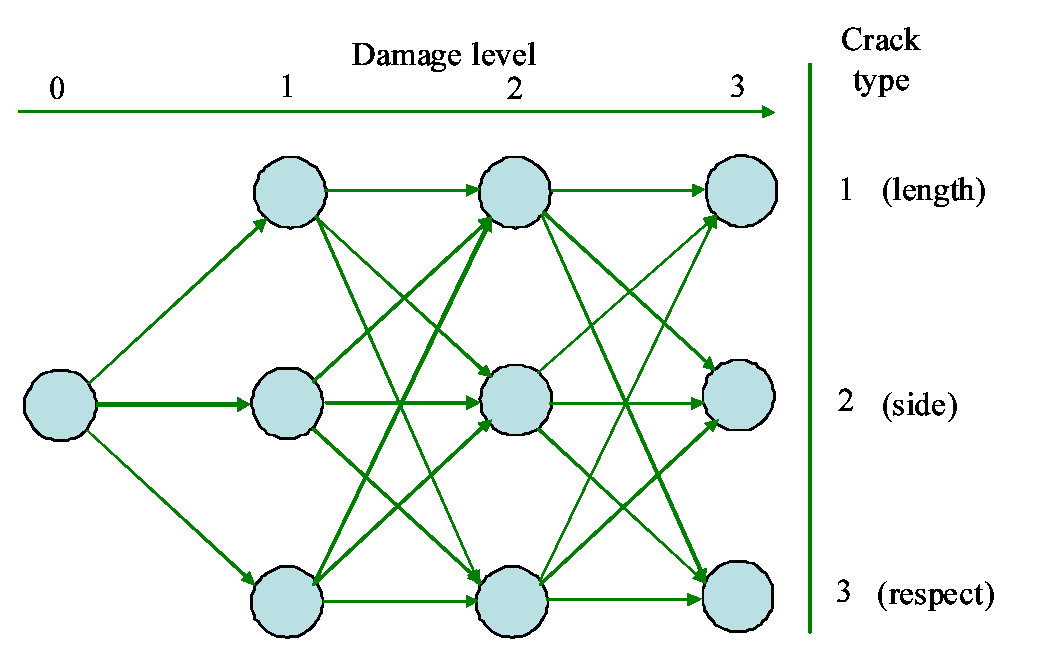
\includegraphics[scale=0.5]{fig27.eps} 
\end{center}
\footnotesize Note) $\bigcirc$ represents deterioration condition state. Deterioration is expressed as a pair ($i,j$). $i$ is referred to damage level $i(i=0,1,2,3)$ while $j$ denotes the crack type $j(j=1,2,3)$. The cracking progresses by mean of pattern transition from deterioration state $(0,0)$ to the right side of the figure.
\caption{The Process of Cracking Progress in Pavement System.}
\label{fig27} 
\end{figure}
%%%%
\begin{eqnarray}
\prod { = \left( {\begin{array}{*{20}c}
   {\pi _{00} } &  \cdots  & {\pi _{0L} }  \\
    \vdots  &  \ddots  &  \vdots   \\
   o &  \cdots  & {\pi _{LL} }  \\
\end{array}} \right)} \hspace{1mm}.\label{pi35}
\end{eqnarray}
%
where $o$ is $0$ element procession in the left low triangular of the transition matrix, $\pi_{il}(i,l=1,...,L)$ is a block procession with their components as follows:
\begin{eqnarray}
\begin{array}{l}
 \pi _{00}  = \pi _{00,00} \hspace{1mm}, \\ 
 \pi _{0l}  = (\pi _{00,l1}  \cdots \pi _{00,lR} ) \hspace{1mm},\\ 
 \pi _{il}  = \left( {\begin{array}{*{20}c}
   {\pi _{i1,l1} } &  \cdots  & {\pi _{i1,lR} }  \\
    \vdots  &  \ddots  &  \vdots   \\
   {\pi _{iR,l1} } &  \cdots  & {\pi _{iR,lR} }  \\
\end{array}} \right)\hspace{1mm}. \\ 
 \end{array}
\end{eqnarray}

We admit the fact that the property of Markov transition probability in equation (\ref{pi35}) will change its value if having any change in the duration of inspection interval. In addition, in the situation that no maintenance and repair activities have been implemented in the period between two inspections, deterioration will progress, and the transition probability will satisfy conditions $\pi_{ij,lr}=0 (i > l)$, $\sum\nolimits_{l = i}^L {\sum\nolimits_{r = 1}^R {\pi _{ij,lr} } }  = 1$:
%
\begin{eqnarray}
\begin{array}{l}
  \left. {\begin{array}{*{20}c}
   {\pi _{ij,lr}  \ge 0}  \\
   {\pi _{ij,lr}  = 0 \hspace{2mm} (when \hspace{2mm} i > l)} \\
   {\sum\nolimits_{l = i}^L {\sum\nolimits_{r = 1}^R {\pi _{ij,lr} } }  = 1}  \\
\end{array}} \right\} \hspace{1mm}.\\ 
 \end{array} \label{pt36}
\end{eqnarray}
The pair of state $(L,r)$ $(r=1,...,R)$ is understood as absorbing pair of condition states with its Markov transition probability $\pi _{Lr,Lr}$ if the condition for no maintenance and repair in the history hold.

Let us consider the transition from the pair of condition state $(i,j)$ to $(i+1,r)$. The hazard rate is the summation of transition intensity $\rho _{ijr}$ being counted in the entire domain of $r$:
\begin{eqnarray}
\theta _{ij}  = \sum\limits_{r = 1}^R {\rho _{ijr} } \hspace{1mm}.\label{tranintent}
\end{eqnarray}
 %%%%%%%%%%
\subsubsection{The Hierarchical Hazard Model Formulation}
\label{2422}
In this section, we explained the procedure to formulate the transition probability of hierarchical hazard model in the assumption that observed condition states at inspection time $t=\tau_A$, $t=\tau_B$ are $h(\tau_A)=(i,j)$ and $h(\tau_B)=(l,r)$ with inspection interval $Z=\tau_B-\tau_A$.
\begin{itemize}
\item{When $(i,j)=(l,r)$}
\end{itemize}
In this case, over the period between two inspections, there has been no sign of deterioration. The original pair of condition states $(i,j)$ remains. By a similar provision to equation (\ref{pro1}), the Markov transition probability for the pair of condition state $(i,j)$ remains in the duration $Z$ can be defined:
\begin{eqnarray}
\pi_{ij,ij}(Z)=exp(-\theta_{ij}Z)\hspace{1mm}.
\end{eqnarray}
At absorbing state ($i=L$), the probability of transition absolutely equals to 1 ($\pi_{Lj,Lj}(Z)=1$).
\begin{itemize}
\item{When $l=i+1 \leq L-1$}
\end{itemize}
In this case, the damage level changes from $\tau_A=i$ to $\tau_B=i+1$ with its transition frequency of $1$. While, the damage type (cracking form in PMS as an instance), may vary in the range of $R$ ($R$ is absorbing state for damage type). Thus, we obtain the probability density function of the transition:
\begin{eqnarray}
f_{ij} (\zeta _{ij} ) = \theta _{ij} \exp ( - \theta _{ij} \zeta _{ij} ) = \sum\limits_{r = 1}^R {\rho _{ijr} \exp ( - } \theta _{ij} \zeta _{ij} )\hspace{1mm},
\end{eqnarray}
where $\zeta_{ij}$ is the life expectancy of condition state $i$. $\rho_{ijr}$, as described earlier in equation (\ref{tranintent}), is transition intensity with respect to the change of condition state from $(i,j)$ to $(i+1,j)$. The change of condition state from $(i,j)$ to $(i+1,r)$ in the interval of inspection $[\tau_A,\tau_B)$ can  happen at any arbitrary time. In another word, it is understandable to say the deterioration may shift from time $\tau_A$ to time $s_{i+1}=\tau_A+z_{ij}, (z_{ij}\in [0,Z]$, and from that time onward till the next inspection time $\tau_B$, condition state $(i+1,r)$ remains.

Further to the change of deterioration from pair $(i,j)$ to pair $(i+1,r)$, it is obvious to say that an accurate time, at which, the change happened, can not be defined in a deterministic way. Only possible way to simulate the process is to assume the transition of condition state happens at time $(\tau_A+\bar z_{ij})\in [\tau_A,\tau_B)$. With this assumption, it is understandable that the pair of condition state $(i,j)$ remains from the inspection time $\tau_A$ until arbitrary time $\tau_A+\bar z_{ij}$ in $(i,j)$ before reaching to a new pair of condition state $(i+1,r)$. It is possible therefore to express the conditional probability density $g_{ijr}(\bar z_{ij})$, at which, happening the change of the pair of condition state from  $(i,j)$ to $(i+1,r)$ at time $\tau_A+\bar z_{ij}$:
%%%%
\begin{eqnarray}
&& g_{ijr} (\bar z_{ij} ) = \frac{{\rho _{ijr} }}{{\theta _{ij} }}\frac{{f_{ij} (z_{ij}  + \tau _A )}}{{\tilde F_{ij} (\tau _A )}} \nonumber \\ 
&& = \frac{{\rho _{ijr} \exp \{  - \theta _{ij} (\bar z_{ij}  + \tau _A \} }}{{\exp ( - \theta _{ij} \tau _A )}} = \rho _{ijr} \exp (\theta _{ij} \bar z_{ij} )\hspace{1mm}.
\end{eqnarray}
Additionally, if the entire inspection duration $Z$ is considered. The conditional probability density $q_{ijr} (\bar z_{ij})$ (at which the condition state $(i+1,r)$ remaining until inspection time $\tau_B$) can be expressible by means of the joint probability between the conditional probability $g_{ijr}(\bar z_{ij})$ and the survival probability $\tilde F_{i + 1,r} (\tau _B - \bar z_{ij} - \tau _A )$:
%%%%
\begin{eqnarray}
\begin{array}{l}
 q_{ijr} (\bar z_{ij} ) = g_{ijr} (\bar z_{ij} ) \cdot \tilde F_{i + 1,r} (\tau _B  - \bar z_{ij}  - \tau _A ) \\ 
  = \rho _{ijr} (\bar z_{ij} )\exp ( - \theta _{ij} \bar z_{ij} )\exp \{  - \theta _{i + 1,r} (Z - \bar z_{ij} )\}  \\ 
  = \rho _{ijr} (\bar z_{ij} )\exp ( - \theta _{i + 1,r} Z)\exp \{  - (\theta _{ij}  - \theta _{i + 1,r} )\bar z_{ij} \}  \hspace{1mm}.\\ 
 \end{array} \label{eq248}
\end{eqnarray}
In equation (\ref{eq248}), the elapsed time $\bar s_{i+1}=\tau_A+\bar z_{ij}$ is considered as a fixed term. However, as a matter of course, the change of pair of condition state can happen at any arbitrary time $z_{ij}$ within the inspection interval $Z$. Hence, the Markov transition probability $\pi_{ij,i+1r}$, to which, the deterioration progresses from $(i,j)$ to $(i+1,r)$ in between the two consecutive inspection times is just the integration of conditional probability $q_{ijr} (\bar z_{ij} )$ in continuous time frame:
%%% 
\begin{eqnarray}
\begin{array}{l}
 \pi _{ij,i + 1r} (Z) = {\rm{Prob}}[h(\tau _B ) = (i + 1,r)|h(\tau _A ) = (i,j)] \\ 
  = \int\limits_0^Z {q_{ijr} (z_{ij} )dz_{ij} }  = \int\limits_0^Z {\rho _{ijr} \exp ( - \theta _{i + 1r} Z)\exp \{  - (\theta _{ij}  - \theta _{i + 1r} )z_{ij} \} dz_{ij} }  \\ 
  = \frac{{\rho _{ijr} }}{{\theta _{ij}  - \theta _{i + 1r} }}\{  - \exp ( - \theta _{ij} Z) + \exp ( - \theta _{i + 1r} Z)\}  \hspace{1mm}.\\ 
 \end{array} \label{eq250}
\end{eqnarray}
In equation (\ref{eq250}), regardless of how positive or negative in the relation between $\theta_{ij}$ and $\theta_{i+1r}$ is, the value of Markov transition probability is always positive $ \pi_{ij,i+1r} > 0$.

Regarding the estimation for Markov transition probability $\pi_{ij,lr}$, a similar probabilistic inference and calculation can be derived for a general case. Details has already explained in subsection \ref{241}. The following subsection briefly describes the estimation method for useful connection.
%%%%
\subsubsection{Estimation method for hierarchical index deterioration hazard model}
\label{2423}
The obtained inspection information on sample $k$ can be described as $\bar\xi^k=(\bar \delta^k,\bar Z^k,\bar x^k)$ with the sign $\left[ {\bar {\hspace{3mm}} } \right]$ inferring an actual measurement value. $\bar \delta^k$ is an additional dummy variable receiving its value of $1$ if $h(\tau_A^k)=(i,j)$ and $h(\tau_B^k)=(l,r)$, otherwise, its value is assumed to be equal to $0$. The transition intensity $\rho_{ijr}^k (i=0,...,L-1;r=0,...,R;k=1,...,K)$, which forms a part of Markov transition probability, can be expressible through the peculiar characteristic vector $x^k$ and the unknown parameter $\beta_{ijr}$:
\begin{eqnarray}
\rho _{ijr}^k  = x^k \beta _{ijr}^{'} \hspace{1mm}.
\end{eqnarray}
Moreover, since the inspection interval $\bar Z^k$ also effects on the change of Markov transition probability $\pi_{ij,lr}$, we can express the transition probability in the functional form $\pi_{ij,lr}(\bar Z^k, \bar x^k: \beta)$. $(\bar Z^k, \bar x^k)$ is measured by inspection and $\beta=(\beta_{000},...,\beta_{L-1RR})$ is vector of unknown parameter deeming to be estimated. If assuming the mutually independence of occurrence of condition state on total $K$ samples, we are able to express the simultaneous probability density by means of log-likelihood function as follow:
%%%%%%
\begin{eqnarray}
\begin{array}{l}
 \ln \ell (\beta ) = \ln \prod\limits_{i = 0}^{L - 1} {\prod\limits_{j = 0}^R {\prod\limits_{l = i}^{L - 1} {\prod\limits_{r = 0}^R {\prod\limits_{k = 1}^K {\left\{ {\pi _{ij,lr} (\bar Z^k ,\bar x^k :\beta )} \right\}} } } } } ^{\bar \delta _{ij,lr}^k }  \\ 
  = \sum\limits_{i = 0}^{L - 1} {\sum\limits_{j = 0}^R {\sum\limits_{l = i}^{L - 1} {\sum\limits_{r = 0}^R {\sum\limits_{k = 1}^K {\bar \delta _{ij,lr}^k } } } } } \ln \left\{ {\pi _{ij,lr} (\bar Z^k ,\bar x^k :\beta )} \right\} \hspace{1mm}.\\ 
 \end{array}
\end{eqnarray}
This log-likelihood function defines that it is a function of unknown parameter $\beta$ given observational data $\bar \delta_{ij,lr}^k, \bar Z_k, \bar x^k$. Solution approach using maximum likelihood estimation to this function is similar to the approach that has already explained in section \ref{2413}.
%%%%%%%%%%%%%%%
\section{Hazard Model with Bayesian Estimation}
\label{25}
\subsection{Necessity of Bayesian estimation}
\label{251}
There are a vast number of references on Bayesian estimation worldwide. Especially, in statistic and probability area, the method in Bayesian estimation turns out to be among the powerful tool for estimation of statistical and probabilistic models under constrains of sampling population. Bayesian estimation uses the collected prior information on the behavior of event to update the probability of occurrence of event in the future \cite{wago}.

From the standpoint of infrastructure asset management, Bayesian estimation, without any doubt, indeed becomes of necessity since it is often the case that we have to estimate the model's parameters under the umbrella of small sampling data \cite{fenghong,ben-akiva93,ben-akiva95}. In addition, measurement errors and bias in observed inspection data have been reported as significant factors, which appear to violate the accuracy of estimation \cite{mishalanigong}. 
%%

Let us have a look at the \textbf{Figure \ref{fig28}} to understand the principle of powerful Bayesian estimation for infrastructure asset management. The figure illustrates three different situations when Bayesian principles are applied. Level of accuracy of hazard model will increase if plenty of prior information and observed data is available. The estimation results are thought to be improved as moving the estimation procedure on the right hand side of the Figure.

In reality, it is extremely important to apply Bayesian update rule. For examples, technology innovation in infrastructure asset would probably change the behavior of deterioration process (maintenance, repair, renovation with new technology). Thus if only relies on the past inspection without considering the changes, a wrong result may be encountered as a consequence. In another perspective, applying Bayesian estimation, we can utilize the expertise and the vast rich knowledge, which has been constantly accumulated throughout the years. As a result, we can minimize the subjective assumption in prior information.
\begin{figure}[t]
\begin{center}
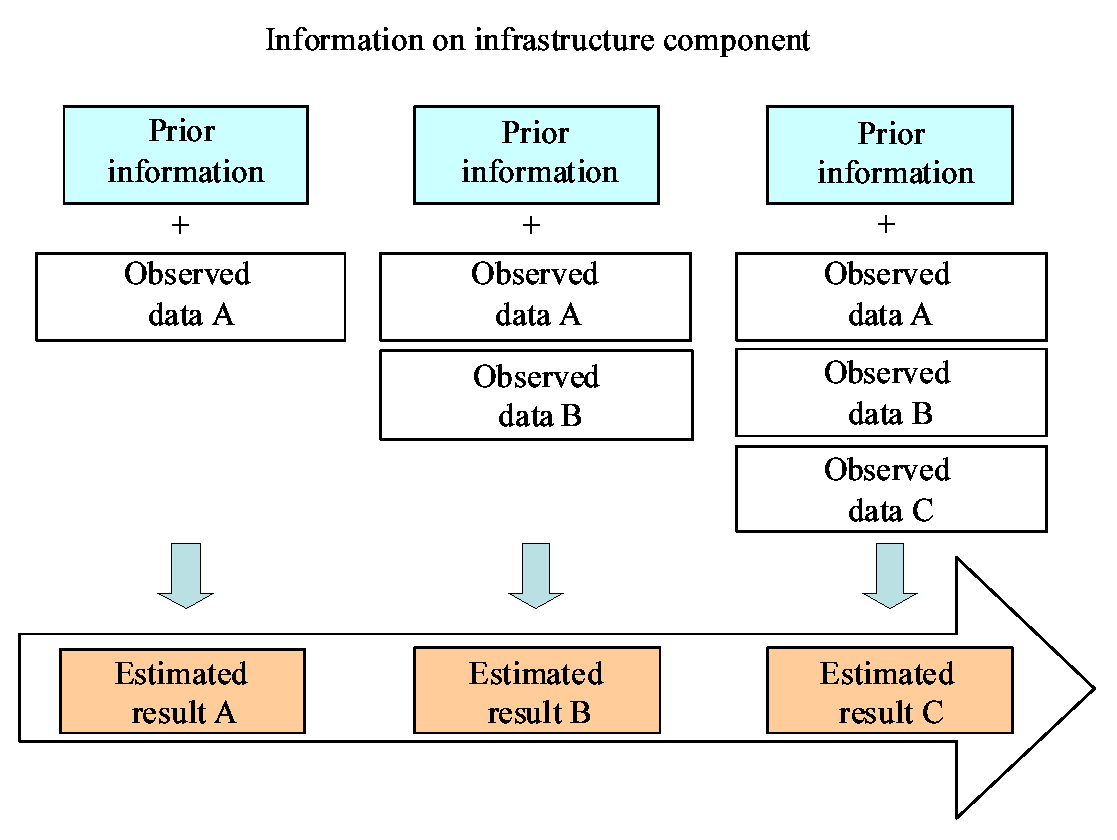
\includegraphics[scale=0.5]{fig28} 
\end{center}
\footnotesize Note) Bayesian update is applied at respective stages when having new observed data. As the sequent, accuracy level happens to increase. Moreover, the influence of prior subjective information will be weakening throughout the time.
\caption{Bayesian Update Principle Chart.}
\label{fig28} 
\end{figure}
%%%
\subsection{Bayesian estimation and its prior subjective information}
\label{252}
Maximum likelihood estimation approach, as described in section \ref{24}, is an excellent approach to estimate the model's parameter under the circumstance that numerous data has been accumulated. The reason behinds that is, as a probabilistic approach, maximum likelihood estimation illustrates the behavior of distribution of parameter around the mean. In another word, the asymptotic behavior can only be acquired if huge number of data is available. 

However, in many cases, it is hard to have a full set of sufficient data. And thus, if continuing with maximum likelihood approach, the bias in estimation results may occur, especially under data insufficiency. Furthermore, there happens a high possibility that measurement errors and bias actually exist within the sampling population. It is therefore, when Bayesian estimation is applied with use of the prior information, the estimation results can be greatly improved.

In Bayesian estimation, the posterior distribution of the parameter will be estimated by using the likelihood function defined by the employing prior distribution of parameter and observed data \cite{andrwewgel}. The likelihood function is denoted as $\iota( \left. {\theta} \right|\xi)$ with  $\theta$ and $\xi$ respectively inferring unknown parameter and observed data. Based on Bayesian theorem, the unknown parameter $\theta$ is assumed to be a random variable and the Bayesian posterior probability $\pi (\left. {\theta} \right|\xi)$ of $\theta$ given observed data $\xi$ can be defined as
%%%
\begin{eqnarray}
\pi (\left. \theta  \right|\xi ) = \frac{{\ell (\left. \theta  \right|\xi )\pi (\theta )}}{{\int_\Theta  {\ell (\left. \theta  \right|\xi )\pi (\theta )d\theta } }}, \label{bayesi}
\end{eqnarray}
where $\pi (\theta )$ is the prior probability of $\theta$ that was inferred before new evidence becoming available. The sign $\Theta$ denotes the space of unknown parameter. In some extend, it is understandable to approximate $\pi (\left. {\theta} \right|\xi)$ to the value of the nominator in equation (\ref{bayesi}):
\begin{eqnarray}
\pi (\left. \theta  \right|\xi ) \propto \ell (\left. \theta  \right|\xi )\pi (\theta ). \label{pibayesian}
\end{eqnarray}
The denominator in equation (\ref{bayesi}) is regarded as a constant term inferring the standard or the prior predicted distribution of $\pi (\left. {\theta} \right|\xi)$.:
\begin{eqnarray}
m(\xi ) = \int_\Theta  {\ell (\left. \theta  \right|\xi )\pi (\theta )d\theta }. 
\end{eqnarray}
In Bayesian updating rule, the steps of estimation are as follows: 1) Assuming the prior probability density function $\pi(\theta)$ based on the prior experience information, 2) Defining the likelihood function $\ell (\left. \theta  \right|\xi )$ based on newly observed data $\xi$, 3) Updating the probability density function $\pi (\left. {\theta} \right|\xi)$ for the parameter $\theta$ based on the Bayesian rule in equation (\ref{bayesi}). In this method, the probability distribution of unknown parameter $\theta$ is not estimated in the same way like that by using maximum likelihood estimation, but by Bayesian updating rule in the condition of obtaining the posterior distribution.
%%%%%
\subsection{Markov Chain Monte Carlo Simulation}
\label{253}
In general, there is a limitation in estimating parameter of deterioration hazard model either with maximum likelihood and Bayesian updating rule if the problem of multi-integration exists \cite{wago,titter,robert}. In recent years, Markov Chain Monte Carlo (MCMC) has been introduced in the field of Bayesian statistics, and as the sequent, greatly improve the estimation for posterior distribution without considering such a high and sophisticated level of integration \cite{wago}. 

In MCMC simulation, Gibbs sampling and Metropolis Hastings (Metropolis-Hastings or MH) techniques have been remarkably discussed \citep{wago,danihed}. Reference to image restoration was among the first application of MCMC simulation \citep{gibbs1}. Of that study, the algorithm of Gibbs Sampling was used to estimate the posterior distribution in Bayesian estimation \citep{gibbs2}. In MH law, the iterative parameter $\mbox{\boldmath$\theta$}$ is defined by repeatedly generating random numbers through the conditional probability density function $\pi (\left. {\theta} \right|\xi)$.
%%%%%%%%%%%%%
%\subsection{Bayesian estimation for Weibull deterioration hazard model}
%\label{254}
%This part presents an approach to estimate the unknown parameter $\theta$ of Weibull deterioration hazard model using the Bayesian updating rule. Reference is made to subsection \ref{234}. In this case, we assume the newly acquired data as  $\bar (\xi_1,...,\bar \xi_n)$. The likelihood function defined by Weibull distribution in equations (\ref{prop-bFlaw}) and (\ref{kikanw}) is expressed as follow
%%%%%%%%%%%
%\begin{eqnarray}
%\begin{array}{l}
% \ell (\left. \theta  \right|\bar \xi ) = \prod\limits_{i = 1}^n {f(\bar y_i ,\bar x_i :\theta )^{\bar d_i } }  \cdot \tilde F(\bar y_i ,\bar x_i :\theta )^{1 - \bar d_i }  \\ 
% =m^{\bar d} \exp \left\{ {\sum\limits_{i = 1}^n {(\bar d_i \bar x_i \beta ^{'}  + \bar d_i (m - 1)\ln \bar y_i  - \exp (\bar x_i \beta ^{'} )\bar y_i^m } )} \right\} \\ 
% \end{array} \label{ptweibull}
%\end{eqnarray}
%where $\bar d$ means the total number $\bar d = \sum\nolimits_{i = 1}^n {\bar d_i }$ corresponding to the sample, which already changed its life expectancy during the inspection period. $\theta=(m,\beta)$ is unknown parameter in Weibull hazard model. It is noted that the prior density function to likelihood function (\ref{ptweibull}) does not exist. Therefore, the function type of prior probability density function $\pi (\theta)$ and probability density function $\pi (\left. {\theta} \right|\xi)$ are multually independent in Bayesian estimation rule. 
%
%In fact, in Bayesian estimation method, the prior probability density function of parameters $m$ and $\beta$ are assumed to follow probabilistic distribution such as Gamma distribution $m \sim g(m_0 ,\kappa _0 )$ and multi-dimensional normal distribution $\beta  \sim N_k (\mu _o ,\sum\nolimits_o {} )$ respectively. The probability density function of gamma distribution $g(m_0 ,\kappa _0 ), K$ and $K$ dimensions of normal distribution $\sim N_k (\mu _o ,\sum\nolimits_o {})$ are respectively given below.
%%%%%%%
%\begin{manyeqns}
 %&& \hspace{-10mm} f(m|m_0 ,k_0 ) = \frac{1}{{\Gamma (m_0 )}}\kappa _0 ^{m_0 } m^{m_0  - 1} e^{ - \kappa _0 m}  \\ 
% && \hspace{-10mm} g(\beta |\mu o,\sum\nolimits_o {} ) = \frac{1}{{\sqrt {(2\pi )^K |\sum\nolimits_o {} |} }} 
% \exp \left\{ { - \frac{1}{2}(\beta  - \mu _o )\sum\nolimits_o^{ - 1} {(\beta  - \mu _o )^{'} } } \right\} 
%\end{manyeqns}
%where $\sum\nolimits_o$ and $\mu _o$ of $\sim N_k (\mu _o ,\sum\nolimits_o {})$ are the  covariance matrix and the standard covariance of prior distribution respectively. As a result, proportional results of probability density function $\pi (\left. {\theta} \right|\bar \xi)$ expressed in equation \ref{pibayesian} is re-formulated as follows.
%%%%%%%%%%%
%\begin{eqnarray}
%\begin{array}{l}
% \pi (\left. \theta  \right|\bar \xi ) \propto \ell (\left. \theta  \right|\bar \xi )f(m|m_0 ,k_0 )g(\beta |\mu o,\sum\nolimits_o {} ) \\ 
 % \propto m^{m_o  + \bar d - 1} \exp \left\{ {\sum\limits_{i = 1}^n {(\bar d_i \bar x_i \beta ^{'}  + \bar d_i (m - 1)\ln \bar y_i  - \exp (\bar x_i \beta ^{'} )\bar y_i^m } } \right\} - \kappa _0 m \\ 
%  - \frac{1}{2}(\beta  - \mu _o )\sum\nolimits_o^{ - 1} {(\beta  - \mu _o )^{'} }  \\ 
% \end{array} \label{pibaym}
%\end{eqnarray}
%It is assumed at this point that the value of parameter $m$ and $\beta$ are available, thus, the conditional probability density function $\pi (m|\beta, \bar \xi)$ can be defined from equation (\ref{pibaym}).
%\begin{eqnarray}
%\begin{array}{l}
 %\pi (m|\beta ,\bar \xi ) \propto m^{\hat m_o  - 1} \exp ( - \hat \kappa _0 m)\exp ( - \sum\limits_{i = 1}^n {\gamma _i \bar y_i^m } ) \\ 
 %\left\{ {\begin{array}{*{20}c}
 %  {\hat m_0  = m_0  + \sum\nolimits_{i = 1}^n {\bar d_i {\rm{      }}} }  \\
 %  {\hat \kappa _0  = \kappa _0  + \sum\nolimits_{i = 1}^n {\bar d_i \ln \bar y_i } }  \\
  % {\gamma _i  = \exp (\bar x_i \beta ^{'} ){\rm{          }}}  \\
%\end{array}} \right. \\ 
 %\end{array} \label{priorbay}
%\end{eqnarray}
%By updating rule in Bayesian estimation, the value of unknown parameter $\beta^{-j}$ in the pool of elements $\beta^{j}$  $j(j=1,...,K)$, which deems to be revealed, will be excluded from the rest of the vector $\beta$. Thus, a new estimation for $\beta^{j}$ can be realized based on conditional probability density function $\pi (\beta^{j}|m,\beta^{-j},\bar \xi)$ given already-known value of $m$ and $\beta^{-j}$.
%%%%%%%%%%%%%%
%\begin{eqnarray}
%\begin{array}{l}
 %\pi (\beta ^j |m,\beta ^{ - j} ,\bar \xi ) \propto \exp \left\{ { - \frac{{\rho _{jj} }}{2}(\beta ^j  - \hat \mu _0^j )^2 } \right\}\exp ( - \sum\limits_{i = 1}^n {\gamma _i \bar y_i^m } ) \\ 
 %\left\{ {\begin{array}{*{20}c}
 %  {\hat \mu _0^j  = \mu _0^j  + \frac{1}{{\rho _{jj} }}\left\{ {\sum\nolimits_{i = 1}^n {\bar d_i x_i^j } } \right.}  
 %  { - \left. {\sum\nolimits_{k = 1, \ne j}^K {(\beta ^k  - \mu _0^k )\rho _{kj} } } \right\}}  \\
 %  {\gamma _i  = \exp (\bar x_i \beta ^{'} ){\rm{          }}}  \\
%\end{array}} \right. \\ 
 %\end{array} \label{priorbay2}
%\end{eqnarray}
%where $\mu_0^j$ is the mean of the expected value vector $\mu_0^j$ of the multi-dimensional normal distribution $N_K(\mu_0,\sum\nolimits_0)$, which presents the prior distribution. $\rho_{kj}$ is $(k,j)$ element of retrogression row $\sum\nolimits_{0}^{-1}$ of the standard covariance and the covariance matrix. Moreover, the sum $\sum\nolimits_{k = 1,\neq j}^K$ means the total of element starting from $1$ to $K$ without considering the element $j$. The sampling algorithm can be further described in following steps.
%%%
%\begin{itemize}
%\item Step 1) Setting the initial parameter value $\theta^0=(m(0), \beta^1(0),...,\beta^K(0))$ with $i=0$ and selecting $\bar n$ samples.
%\item Step 2) Randomly generating $\theta^{i+1}=(m(i+1), \beta^1(i+1),...,\beta^K(i+1))$ in following manners.\\
%\hspace{5mm} - Randomly generating $m(i+1)$ numbers from $\pi (m|\beta(i), \bar \xi$\\
%\hspace{5mm} - Randomly generating $\beta^1(i+1)$ numbers from  $\pi (\beta^1|m(i+1), \beta^{-1}(i), \bar \xi)$\\
%\hspace{5mm} - Randomly generating $\beta^k(i+1)$ numbers from  $\pi (\beta^k|m(i+1), \beta^1(i+1), ...,$\\$ \beta^{k-1}(i+1), \beta^{k+1}(i),..., \beta^K(i), \bar \xi)$ with $(k=2, ...,K-1)$\\
%\hspace{5mm} - Randomly generating $\beta^K(i+1)$ numbers from $\pi (\beta^K|m(i+1), \beta^{-K}(i+1), \bar \xi)$
%\item Step 3) Accepting  $\theta^{i+1}$ if $i \geq n$.
%\item Step 4) Ending the calculation iteration if  $i=\bar n$. Otherwise, if $i < \bar n$, returning to $Step 2$ and increasing the level $i=i+1$.
%\end{itemize}
%In Gibbs sampling, the definition of nucleus transition $K(\theta^i, \theta^{i+1}|\bar \xi)$ is as follow
%%
%\begin{eqnarray}
%\begin{array}{l}
 %K(\theta ^i ,\theta ^{i + 1} |\bar \xi ) = \pi (m(i + 1)|\beta (i),\bar \xi )\prod\limits_{j = 1}^{K - 1} {\pi (\beta ^j (i + 1)} |m(i + 1), \\ 
 %\beta ^1 (i + 1),...,\beta ^{j - 1} (i + 1),\beta ^{j + 1} (i),...,\beta ^K (i),\bar \xi ) \cdot \\ \pi (\beta ^K (i + 1)|m(i + 1),\beta ^{ - K} (i + 1),\bar \xi ) \\ 
 %\end{array}
%\end{eqnarray}
%In this understanding, the value of $\theta^i (i=0,1,...)$ is thought to follow Markov chain with its nucleus transition $K(\theta^i, \theta^{i+1}|\bar \xi$. In addition, $\theta^i (i=n+1, n+2, ..., n)$ obtained by Gibbs sampling can be regarded as specimen sample from probability density function $\pi (\theta |\bar \xi)$, at which, satisfying the stationary state of Markov chain for a very big $n$. 
%
%After $K+1$ samples, it is possible to obtain the conditional probability density function $\pi (m|\beta, \bar \xi)$ and $\pi (\beta^j|m, \beta^{-j}, \bar \xi)(j=1,...,K)$. When the equations (\ref{priorbay}) and (\ref{priorbay2}) are considered as functions of $m$ and $\beta^j(j=1,...,K)$, then both log-likelihood functions $ln[\pi(m|\beta ,\bar \xi)]$ and $ln[\pi (\beta^j|m, \beta{-j},\bar \xi)] (j=1,...,K)$ are concave functions. It is thus, adaptive dismissal sampling becomes effectively in selecting the specimen sample from posterior distribution since having the concave shapes of probability density function. %%%%%%%%%%% 
%\subsection{Bayesian estimation for Markov hazard model}
%\label{255}
%Bayesian estimation can also be applied to estimate the unknown parameter $\beta$ of the exponential Markov deterioration hazard model, which is discussed in section \ref{241}. The rule of Bayesian estimation is carried out by using the visual inspection data of the second time. We denote $\bar \xi = (\bar \xi^1,...,\bar \xi^K)$ as the information of newly inspection data, which comprises of the information on sample $k$ as $\bar \xi^k = (\bar \delta_{ij}^k, \bar z^k, \bar x^k)$. Thus, from equation (\ref{hazardpiij}) and (\ref{logbF}), the likelihood function of exponential Markov hazard model can be re-written as
%\begin{eqnarray}
%\ell (\beta |\bar \xi ) = \prod\limits_{i = 1}^{J - 1} {\prod\limits_{j = 1}^J {\prod\limits_{k = 1}^K {\left\{ {\sum\limits_{h = i}^j {\prod\limits_{l = i}^{h - 1} {\frac{{\theta _l^k }}{{\theta _l^k  - \theta _h^k }}\prod\limits_{l = h}^{j - 1} {\frac{{\theta _l^k }}{{\theta _{l + 1}^k  - \theta _h^k }}} } } \exp ( - \theta _h^k \bar z^k )} \right\}^{\bar \delta _{ij}^k } } } } 
%\end{eqnarray}
%A standard prior probability density function of $\beta_i$ is assumed to follow multi-dimensional normal distribution $\beta_i \sim N_M(\mu_i, \sum\nolimits_{i})$. As a result, it is possible to express the probability density function $\pi (\beta|\bar \xi)$ in view of Bayesian updating rule.
%\begin{eqnarray}
%\begin{array}{l}
% \pi (\beta |\bar \xi ) \propto \ell (\beta |\bar \xi )\prod\limits_{i - 1}^{J - 1} {g(\beta |\mu _i ,\sum\nolimits_i {} )}  \\ 
 % \propto \prod\limits_{i = 1}^{J - 1} {\prod\limits_{j = 1}^J {\prod\limits_{k = 1}^K {\left\{ {\prod\limits_{l = i}^{j - 1} {\theta _l^k \sum\limits_{h = i}^j {\prod\limits_{l = i}^{h - 1} {\frac{1}{{\theta _l^k  - \theta _h^k }}\prod\limits_{l = h}^{j - 1} {\frac{1}{{\theta _{l + 1}^k  - \theta _h^k }}} } } } \exp ( - \theta _h^k \bar z^k )} \right\}^{\bar \delta _{ij}^k } } } }  \cdot  \\ 
 %\prod\limits_{i = 1}^{J - 1} {\exp \left\{ { - \frac{1}{2}(\beta _i  - \mu _i )\sum\nolimits_i^{ - 1} {(\beta _i  - \mu _i )^{'} } } \right\}} \\ 
 %\end{array} \label{markovbay}
%\end{eqnarray}
%In this sampling rule, the unknown parameter vector $\theta_{e,m}$, of which, values are excluded from $\theta$, is denoted as $\theta_{-(e,m)}$. In view of conditional probability, the probability density function $\pi (\theta_{e,m}|\theta^{-(e,m)}, \bar \xi)$ can be again expressed as follow
%\begin{eqnarray}
%\begin{array}{l}
% \pi (\beta _{e,m} |\beta ^{ - (e,m)} ,\bar \xi ) \propto \\ \prod\limits_{i = 1}^e {\prod\limits_{j = e}^J {\prod\limits_{k = 1}^K {\left\{ {\theta ^{k^{\bar \delta _{ij}^k  - \bar \delta _{ie}^k } }  \cdot \sum\limits_{h = i}^j {\prod\limits_{l = i}^{h - 1} {\frac{1}{{\theta _l^k  - \theta _h^k }}\prod\limits_{l = h}^{j - 1} {\frac{1}{{\theta _{l + 1}^k  - \theta _h^k }}\exp ( - \theta _h^k \bar z^k )} } } } \right\}} } } ^{\bar \delta _{ij}^k }  \\ 
 % \cdot \exp \left\{ { - \frac{1}{2}(\beta _e  - \mu _e )\sum\nolimits_e^{ - 1} {(\beta _e  - \mu _e )^{'} } } \right\}  
 % \propto \\ \prod\limits_{i = 1}^e {\prod\limits_{j = e}^J {\prod\limits_{k = 1}^K {\left\{ {\exp (\beta _{e,m} x_m^k )^{\bar \delta _{ij}^k  - \bar \delta _{ie}^k }  \cdot \sum\limits_{h = i}^j {\prod\limits_{l = i}^{h - 1} {\frac{1}{{\theta _l^k  - \theta _h^k }}\prod\limits_{l = h}^{j - 1} {\frac{1}{{\theta _{l + 1}^k  - \theta _h^k }}\exp ( - \theta _h^k \bar z^k )} } } } \right\}^{\bar \delta _{ij}^k } } } }  \\ 
 % \cdot \exp \left\{ { - \frac{{\rho _e^{mm} }}{2}(\beta _{e,m}  - \hat \mu _e^m )^2 } \right\} \\ 
% \hat \mu _e^m  = \mu _e^m  + \sum\limits_{h = 1, \ne m}^M {(\beta _{e,h}  - \mu _e^h )} \rho _e^{mm}  \\ 
% \end{array}
%\end{eqnarray}
%In this conditional probability density function, value of $\beta_{e,m}$ is thought to conditionally depend on $\beta^{-(e,m)}$, which has already revealed from equation (\ref{markovbay}). $\delta_{ie}^k$ is the dummy variables receiving its value of $1$ when prior rating $e$ is obtained from Gibbs sampling with prior rating $d(\tau_A^k)=i$ on the sample $k$, otherwise value of the dummy variable equals to $0$. $\mu_e^m$ is the median of the prior expected value vector $\mu_e$. $\rho_e^{hm}$ is $(h,m)$ element of the prior standard covariance of procession $\sum\nolimits_{e}^{-1}$. In addition, $\sum\nolimits_{h=1,\neq m}^{M}$ is the sum of total elements counting from $1$ to $K$, excluding element $m$. The specimen is randomly generated from conditional probability density functions. And thus, the generated specimen can be used to infer the posterior distribution of the unknown parameter $\beta$. 
%%%%
%\section{Hazard model and measurement errors}
%\label{26}
%\subsection{Sample loss and measurement errors}
%\label{261}
%Actual application of deterioration hazard model requires data from monitoring. For instance with Markov model, at least two set of inspection data in two different time series are needed to configure the matrix of Markov transition probability. Thus, the accuracy of estimation depends largely on how accurate level of data gathered from inspection is. If measurement errors or bias exist in the measurement, result from estimation has tendency to differ from what actually progress in the reality. Measurement errors and bias can possibly occur due to mistakes of either inspectors or monitoring equipments as well as bias assumption of condition states. Thus, the problem of measurement errors occurring in hazard model due to bias data shall be well addressed.

%Condition state of infrastructure system is often evaluated by use of average or weighted values from various indexes measured by monitoring and inspection activities. For example, in pavement management system (PMS), the Pavement Condition Index  (PCI)\footnote{PCI is a standard performance indicator, which is widely applied in the America. Other similar performance indictors have also applied in other developed countries. For example, MCI (Maintenance Control Index) is used in the PMS of Japan. The definition of PCI or MCI is largely depending on management perspective of each country.} is the weighted value of cracking, international roughness index (IRI), flatness, etc \citep{shahin05}. However, because of the measurement errors, true condition state may not be captured. Let us have a look in to the description of Figure \ref{fig29}, as an example in PMS, for better understanding of the issue.
%\begin{figure}[t]
%\begin{center}
%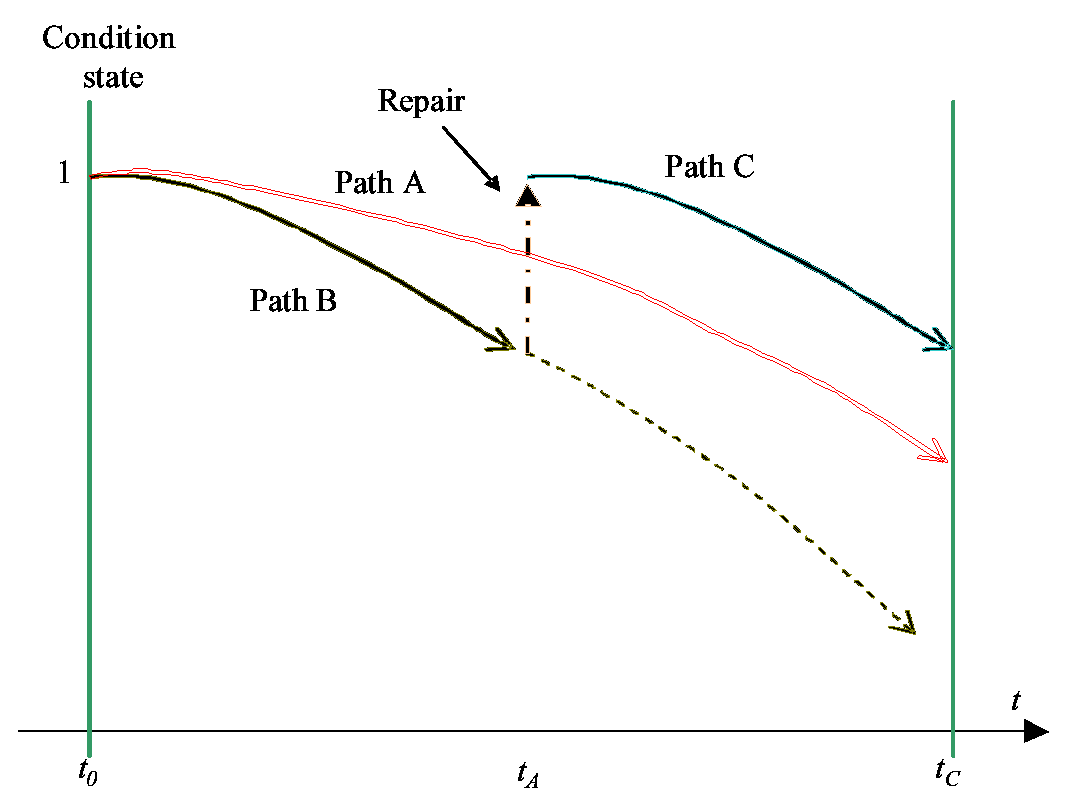
\includegraphics[scale=0.5]{fig29} 
%\end{center}
%\caption{Sample loss and measurement error due to repair}
%\label{fig29} 
%\end{figure}
%
%It is assumed in the figure that at time $\tau_0$, repair is carried out to renew the condition state of pavement to level $1$. If no other repair is carried throughout the period from $\tau_0$ to $\tau_C$, the deterioration curve is likely to follow Path A. In fact, the deterioration progress actually get worsen, and thus, the deterioration progresses like in Path B. In this condition, at time $\tau_A$, repair is imposed and deterioration curve becomes Path C. As the matter of course, if no repair is implemented at $\tau_A$, the deterioration curve will be illustrated in dotted line. However, from the monitoring and measurement standpoint, we only have information at inspection time $\tau_C$. Whereas, the information on repair has not been properly recorded. This type of problem negatively results in inaccurate estimation results of the hazard model.
%
%\begin{figure}[t]
%\begin{center}
%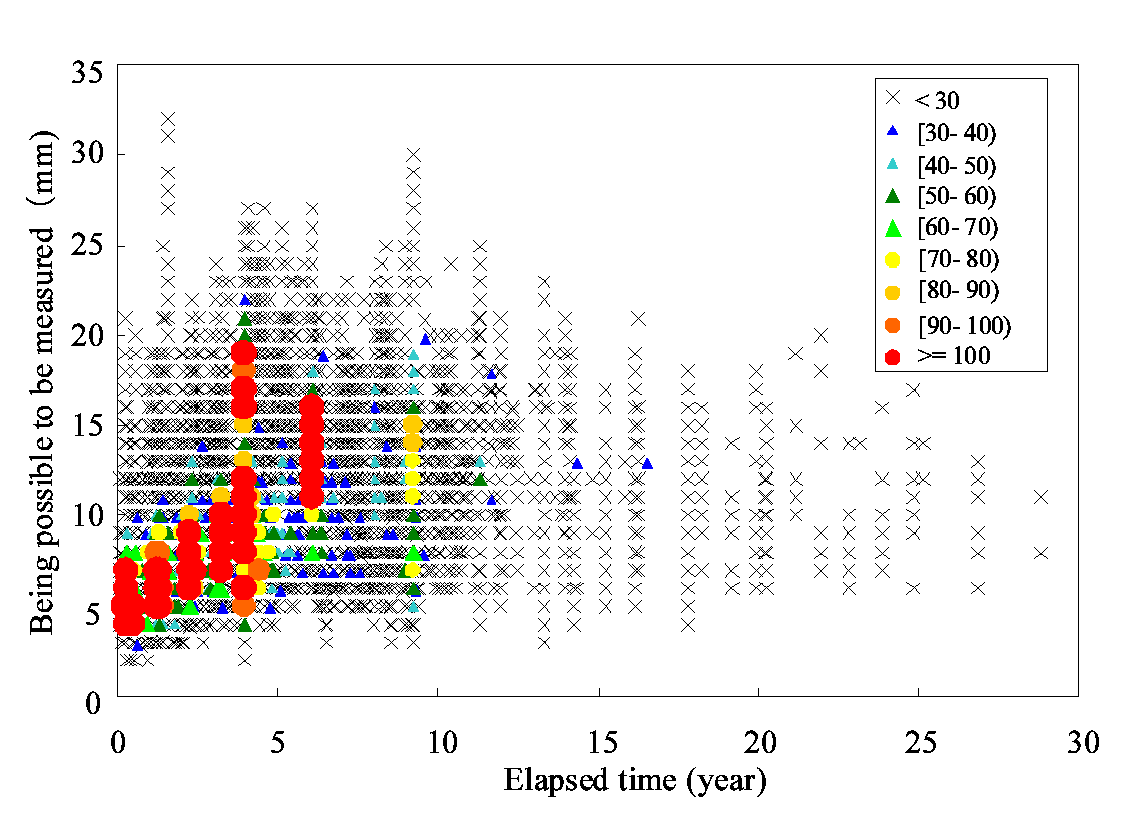
\includegraphics[scale=0.5]{fig210} 
%\end{center}
%\caption{Distribution of measurement sample-rut index (mm)}
%\label{fig210} 
%\end{figure}
%Figure \ref{fig210}, on another perspective, illustrates the problem of measurement errors. The horizontal axis shows the elapsed years, while the vertical axis expresses the possibility of capturing the rut index of road. In the period of 6 years from the opening of the road, there is an abundant amount of samples being recorded. However, the numbers of sample are slowly decrease along with time. Consequently, loss of sample happen. In reality, the condition states are largely distributed with respect to the elapsed time. A deterministic relation of this distribution may not easy to be figure out. In order to overcome this obstacle, following section further highlights the correcting methodology applying on exponential Markov hazard model in case of measurement errors and sample loss.
%%%%%%%%%%%%%
%\subsection{Maximum likelihood estimation method with sample loss}
%\label{262}
%This subsection presents the estimation method for multi-state exponential hazard model in the case of having sample loss. Particularly, dicussion is in close link to the case of pavement management system. However, as a matter of fact, the methodology can be generalize to other infrastructure types.
%
%Let us continue to drawn the case, to which, observations are conducted on sample $k(k=1,...,K)$ at two respective times $\tau_A^k$ and $\tau_B=\tau_A^k+z^k$ with $z^k$ as inspection interval. The condition state being observed at at $\tau_A^k$ and $\tau_B$ are $h(\tau_A^k)=i^k$ and $h(\tau_B^k)=j^k$ respectively. It is assumed at this state that the mentioned condition states being observed in the period $[\tau_A^k, \tau_B^k]$ are prior condition states of the road sections. Addition to the condition states, the information on characteristic variables $x^k=(x_1^k,...,x_M^k)$ are also available as results of inspections. And moreover, it is acknoledged that condition states and concerning characteristic variables are absolutely recorded for all road sections in the total $K$ sections. In short, inspection information of sample $k$ can be expressible by vector $\bar \xi^k=(\bar h(\tau_A^k),\bar h(\tau_B^k), \bar z^k, \bar x^k)(k=1,...,K)$ with [$\bar{\hspace{2mm}}$] referring to the measureable value.
 %
%In reality, inspection activities are scheduled during the management term. The time of inspection is denoted as $z_n (n=1,...,N)$. The actual numbers of characteristic varialbes being revealed through inspections are $x_l (l=1,...,L)$. Based on the obtained inspection information, it is possible to estimate the so-called ``relative frequency'' $\mu(i,z_n,x_l)$ or relative distribution of sample with its atrribute $(i,z_n,x_l)(i=1,...,J-1;n=1,...,N;l=1,...,L)$. Saying in another words, the relative distribution coefficient is deem as known parameter, which is easily obtained from data. On the other hand, the probability (or likelihood) for the simultaneous occurence of the extracted sample, being with its attribute $(i,j,z_n,x_l)$, can be presumed as likelihood function $f(i,j,z_n,x_l:\beta)$ with unknown paramater $\beta$.
%
%In statistic view, sample loss mechanism is considered to be under the shadow of probabilistic manner, and thus, the sample loss can be defined by the rate of sample loss. The loss of sample generally happens when information concerning early maintenance and repair actions on the road section prior to the next inspection time is not recorded. In fact, maintenance and repair actions are carried out on the road sections exerting with faster deteriorations than predictions. If no M\&R has yet been imposed, the prior initial condition state $i$ will deteriorate into condition state $j$. 
%
%n this situation, we express a set of sample with its pair of condition states $(i,j)(i<j)$ by $\Omega$. The possible number of sub-set $\Omega_{ij}(j=i,...,J;i=1,...,J-1)$ is $(J-1)(J+2)/2$. Another way to express the sample set is throught the union $\Omega=\cap_{i=1}^{J-1}\cap_{j=i}^{J} \Omega_{ij}$ with its empty set denoting as  $\Omega_{ij}\cap\Omega_{i^{'}j^{'}}=\phi((ij)\neq(i^{'}j^{'}))$. As a matter of course, based on the information on observed condition states, it is clear to determine the subset, to which, the sample being considered actually belongs to. Furthermore, we can exclude the sample concerning the road section with implemented M\&R during inspection interval. This sample does not belong to any proper subset of sample, and thus, it can be regarded as a sample loss.
%
%Regarding each sample subset $\Omega_{ij}$, it is understanable to define the conditional probability $Q(z_n,x_l|i,j)$ of simultaneous occurence with respect to inspection time and characteristic variables $(z_n,x_l)$. Such a simultaneous occurence probability is concretly defined for each subset of sample. In another words, the sample mechanism generation is different in each sample subset. 
%
%It is acknowledged that among samples obtained by measurement, there are $N_{ij}$ samples belong to sample subset $\Omega_{ij}$. To express the measurement sample, which is randomly extracted from $N_{ij}$ of the sample subset $\Omega_{ij}$, we use the vector $\xi = (\xi^1,...,\xi^{\bar K})$, where $\sum\nolimits_{i=1}^{J-1}\sum\nolimits_{j=1}^{J}N_{ij}=\bar K$. Due to the existence of sample loss, the sum of $N_{ij}$, which is corresponding to numbers $\bar K$ of samples, only indicate to the road sections without any M\&R during the inspection interval. Further to this matter, it is also strongly noted that the rate concerning the sample extraction is different in each samplem subset. 
%
%Theoritically, if there have been no M\&R, the condition state distribution of road section at time $\tau_B$ shall change depending on the prior condition state $i$ measured at inspection time $\tau_A$. In another words, it is possible to express the dependence distribution by describing it as conditional probability density function $\tilde P(j|i,z_n,x_l:\beta)=\pi_{ij}(z_n,x_l:\beta)$, which concerns the distribution of condition state $j$ depending on prior condition state $i$, the inspection interval $z_n$ and the characteristic variable $x_l$. As the sequent, the dependence distribution of condition state at inspection time $\tau_B=\tau_A+z_n$ can be expressed by means of conditional probability density function $P(j|i,z_n,x_l:\beta)=\pi_{ij}(z_n,x_l:\beta)$ and the distribution $\nu(z_n,x_l|i)$ of prior condition state $i$.
%%%
%\begin{eqnarray}
%\begin{array}{l}
 %\tilde Q(j|i:\beta ) = \sum\limits_{n = 1}^N {\sum\limits_{l = 1}^L {\tilde P(j|i,z_n ,x_l :\beta )\nu (z_n ,x_l |i)} }  \\ 
% (i = 1,...,J - 1;j = 1,...,J) \\ \label{pt57}
 %\end{array}
%\end{eqnarray}
%%%
%With reference to the earlier paragraph of this subsection, we can define the simultaneous probability $f(i,j,z_n,x_l:\beta)$ as follows.
%%%%%%%%%%%%%
%\begin{eqnarray}
%&& f(i,j,z_n ,x_l :\beta ) = \nonumber \\
%&& \tilde Q(j|i:\beta )Q(z_n ,x_l |i,j:\beta )\mu (i) = P(j|i,z_n ,x_l :\beta )\mu (i,z_n ,x_l ) \label{pt58}
%\end{eqnarray}
%%%%%%%%%%
%Equation \ref{pt58} can be further expressed in following equation.
%%%
%\begin{eqnarray}
%Q(z_n ,x_l |i,j:\beta ) = \frac{{P(j|i,z_n ,x_l :\beta )\mu (i,z_n ,x_l )}}{{\tilde Q(j|i:\beta )\mu (i)}} \label{pt59}
%\end{eqnarray}
%%
%The simultaneous probability $Q(z_n,x_l|i,j:\beta)$ expressed in equation \ref{pt59} reflects the conditional probability that the measurement sample concerning $(i,j,z_n,x_l)$ is randomly extracted from the sample subset $\Omega_{ij}$. By employing the definition in equation \ref{pt59}, the problems of sample loss, measurement errors and bias can be eliminated. To further describe the behavior of distribution $\nu(z_n,x_l|i)$ in equation \ref{pt57}, let express the distribution weight $w_{n,l|i}$ concerning the prior condition state $i$ with respect to inspection interval $z_n$ and characteristic variable $x_l$ in the following equation. 
%%%
%\begin{eqnarray}
%w_{n,l|i}  = \frac{{ \# \{ k \in \Omega _i |i^k  = i,z^k  = z_n \hspace{2mm} and \hspace{2mm}  x^k  = x_l \} }}{{ \ne \{ k \in \Omega i|i^k  = i\} }}
%\end{eqnarray}
%
%where $\# \lbrace k|B \rbrace$ describes the number of samples, to which, condition $B$ is satisfied. In another view, it is understood that the sample with attributes $(i^k,z^k,x^k)$ shall be neglected by filtering from the set $\Omega_i=\cup_{j=i}^J\Omega_{ij}$. Thus, theoretically, the condition state distribution $\tilde Q(j|i:\beta)$ can be further defined as follow.
%%
%\begin{eqnarray}
%\tilde Q(j|i:\beta ) = \sum\limits_{n = 1}^N {\sum\limits_{l = 1}^L {w_{n,l|i} \pi _{ij} } } (\bar z_n ,\bar x_l :\beta )
%\end{eqnarray}
%%
%Asking for the measurement sample $\bar \xi =(\bar \xi_1,...,\bar \xi_{\bar K})$, which is randomly extracting from the sample subset $\Omega_{ij}$ based on equation \ref{pt59}, the likelihood functions corresponding to the sample loss or bias elimination can be consequently defined.
% 
%\begin{eqnarray}
%\ln \tilde \ell (\bar \xi ,\beta ) = \sum\limits_{i = 1}^{J - 1} {\sum\limits_{j = i}^J {\left\{ {\sum\limits_{k = 1}^{\bar K} {\bar \delta _{ij}^k \ln \pi _{ij} (\bar z^k ,\bar x^k :\beta ) - N_{ij} \ln \tilde Q(j|i:\beta )} } \right\}} } \label{pt62}
%\end{eqnarray}
%where, as previously mentioned, $N_{ij}$ is the number of measurement samples belonging to sample subset $\Omega_{ij}$. $\bar \delta_{ij}^k$ is a dummy variable, which receives its value of $1$ when condition ($\bar h(\tau_A^k)=\bar i$ and $\bar h(\tau_B^k)=\bar j$) statisfy, otherwise, its value is assumed to equal to $0$. To this points, we can use several numerical method like maximum likelihood estimation to solve the equation \ref{pt62} in order to estimate the expected values of models's parameters.
%%%
\section{Example of Empirical Application to Infrastructure Asset Management}
\label{27}
This section discusses the possibility of applying the hazard model on infrastructure asset management at strategic level. Details of estimation is referred to paper of \citet{aokia}. In his paper, Weibull hazard model is employed to suggest the optimal timing of inspection and figure out the best possible renewal policies on tunnel lighting system, which composes as an important structure of expressway. The study focused on deriving the Markov chain process along with Weibull distribution, and further combined hazard model with life cycle cost analysis based on the existing list of renewal.

This model enables to evaluate for not only renewal cost of an individual lighting lamp (low-pressure sodium lamp) but also its optimal inspection time and the cycle of compulsory renewal. Further more, as a general requirement of management; an amount of necessary fixed cost is also generated based on least life cycle cost estimation. The model can also be extended to incorporate various types of risks in form of economic term like loss of money due to traffic congestion, which results from either incident of lighting lamp or inspection and renewal activities. As the sequent, the problem concerning the trade-off situation for inspection period, fixed cost, renewal cost can be successfully tacked. Thus, administrators can save the budget and effectively manage the system in the end.

As can be seen from Figure \ref{fig211}, administrators are able to predict the probability of survival in general for the entire lighting system. This survival probability (vertical axis) decreases along the operation time (horizontal axis) is estimated by use of equation (\ref{hazardw}) in section \ref{234}. By categorizing the lighting system into several types, it is also possible to compare the deterioration curves among those types. This kind of survival probabilities, deterioration curves, estimated by Weibull hazard model eventually turn out to be the input of life cycle cost evaluation, which is further displayed in Figure \ref{fig212}.
\begin{figure}[t]
\begin{center}
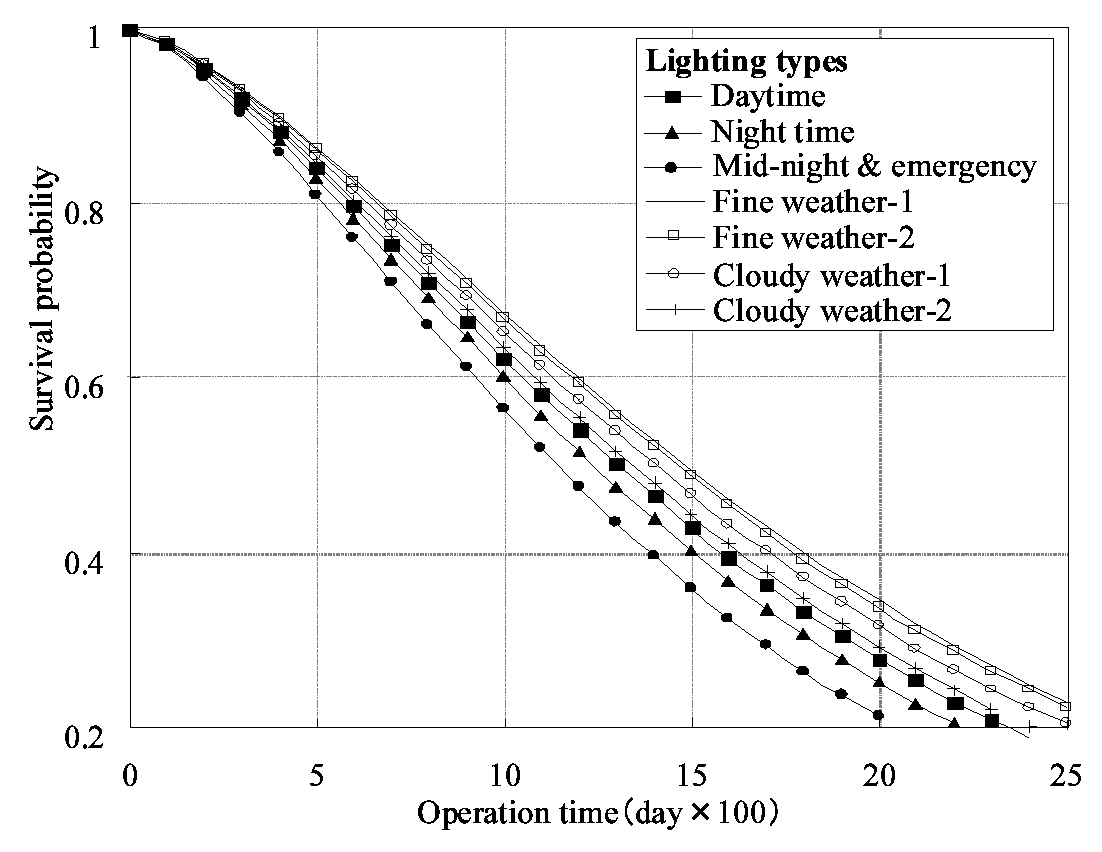
\includegraphics[scale=0.5]{fig211} 
\end{center}
\caption{Survival Probability of Tunnel Lighting Lamp (low-pressure sodium lamp).}
\label{fig211} 
\end{figure}
%%
\begin{figure}[t]
\begin{center}
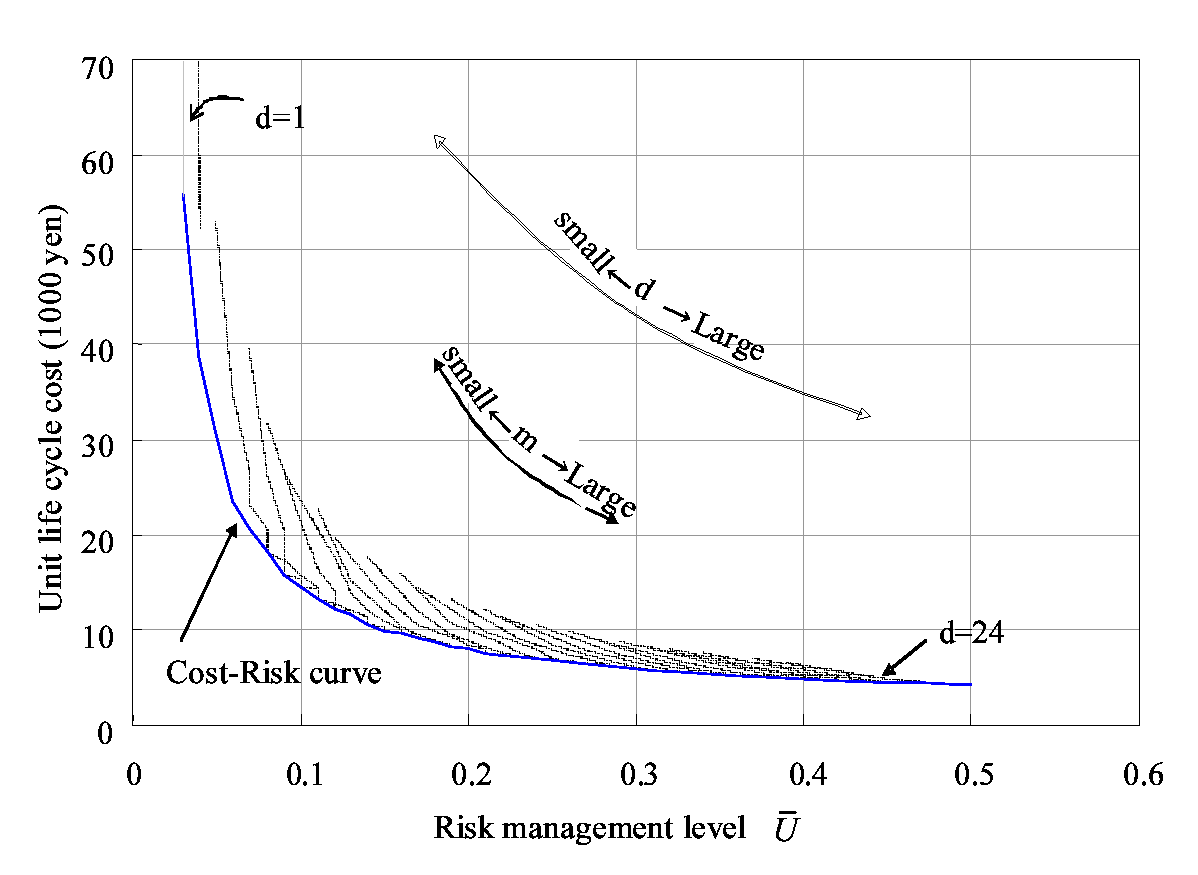
\includegraphics[scale=0.5]{fig212} 
\end{center}
\footnotesize Note) Curve is drawn based on $N=100$ lamps, at the risk management level of 0.05, the C-U curve is showed in dotted line. The solid line explains the C-U relation, which belong to possible management objective.
\caption{Cost-Risk Curve.}
\label{fig212} 
\end{figure}

Figure \ref{fig212} expresses the relation between life cycle cost of tunnel lighting system and the risk management level by drawing the cost-risk curve. The life cycle cost is a summation of inspection cost, inspection cost, renewal cost (if applied) and traffic restriction cost. Whilst, the risk management level is in fact concerning the elapsed time in operation of lighting lamp counting from beginning to the time, at which, encountering the breakdown. In another work, it concerns the so-called Value at Risk (VaR). As can be seen from Figure \ref{fig212}, the relation between trade-off is, as the risk management level grows on the right side of the horizontal axis, then the life cycle cost becomes smaller. In another meaning, the length of inspection interval sketches longer and maximum operation time of lighting lamp is determined. In contrast, as the risk management level becomes smaller than 0.1, the life cycle turns to get an intense upturn. It might be a save option to select the risk management point from 0.2 onward because the variation in change of life cycle cost is in a small scale.
%%%%%%%%%%
\section{Summary and Recommendations}
\label{28}
This chapter has presented a profound literature review on the hazard analysis in infrastructure management system. It strongly emphasized the importance of infrastructure management system in today modern society with its central role, which aims to provide the best service for society systematically. Attention has been given to analytical approach and model formulation based on stochastic methodology. Moreover, the importance role of monitoring and a good inventory box in the system has also been realized throughout the texts. Markov chain model has received a special attention, it possibly become one of a central model for any further extension.

In addition, this chapter has strongly emphasized the application of Bayesian estimation method and Markov Chain Monte Carlo (MCMC) simulation technique. Bayesian estimation combined with MCMC simulation becomes a powerful approach to tackle the issues of limited monitoring sampling data, measurement errors, bias and loss of sample. This would become a very promising horizon for future researches. Moreover, this section has briefly discussed the combination of hazard model and life cycle cost analysis, which is, without any doubt, compulsorily required in any infrastructure management system.

Based on the theory and model discussed in this chapter, the writings and discussion in subsequent chapters of this dissertation will further explore our mathematical formulation of hazard models with empirical studies on selected infrastructure networks such as tunnel lighting system, pavement system and pipeline system.
%%%%%%%%%%%%%%%%
% This is the end of chapter 2 (literature review)
%%%%%%%%%%%%%%%%%

 % Literature Review 

% Chapter 3

\chapter{A Multi-stage Weibull Hazard Model with Tunnel Application} % Write in your own chapter title
\label{Chapter3}
\lhead{Chapter 3. \emph{Multi-stage Weibull Hazard Model with Tunnel Application}} % Write in your own chapter title to set the page header

\section{General introduction}
\label{31}
Effective management of any infrastructure utilities such as tunnel lighting in highway systems requires comprehensive understanding of the entire operational processes of the utility as well as monitoring of its performance and conditions throughout its operational life. Continuous inspection and monitoring of the system are, however, often technically or financially difficult. Therefore, a need to develop an analytical deterioration forecasting model that can estimate the deterioration speed of either an individual component or the entire infrastructure system has been widely recognized. 

Various studies have attempted incorporation of historical background of infrastructure performance into a deterioration model. For example, \citet{aokia} proposed the Weibull distribution function to estimate the deterioration of lighting facilities in tunnel systems. This expressed the condition state of tunnel lighting facilities in binary terms. However, it is known that the actual deterioration process of most infrastructure systems is better described by plural discrete condition states \cite{shahin05}. In order to overcome this limitation, the Markovian transition probability can be used to express two or more condition states in the deterioration process of infrastructure.

The Markov chain model is a stochastic approach that is widely used to forecast the deterioration speed of an infrastructure system such as a bridge network \cite{madanat95,Guido04,Robelin07,Morcous05}. \citet{toukei} and \citet{kobayashitsuda} further improved the Markov chain model by proposing a handy methodology to estimate the Markovian transition probability. The advantages of these models are that they predict future deterioration according to information from two inspection times and they do not  require extensive historical data.

This chapter proposes a new deterioration forecasting model for infrastructure management, which expresses the deterioration speed in two or more condition states in conjunction with elapsed time,  and follows the Weibull distribution function. To begin with, sections \ref{33} and \ref{34} detail the mathematical formulation of the time-dependent transition probability using the Weibull distribution function and the estimation approach. Section \ref{35} presents an empirical study using actual data from a tunnel lighting system in Japan. Finally, the conclusion summarizes the contributions made by this paper, and points out future research needs.
%%%%
%\section{General Background}
%\label{32}
%\subsection{Outline of Literature Review}
%\label{321}
%In the field of infrastructure management, various models on deterioration forecasting have been widely documented. One major feature of the models is to simulate the deterioratoin process. Beside, the models can be ultilized for setting up the maintenance and repair strategies as well as proposing life cycle cost analysis. Especially, under requirement of infrastructure management at network level, these objectives is particular imperative \citep{aokia,kobayashitsuda}.
%
%Many past researches had paid much attention to the physical mechanism of deterioration  of structures \cite{mishalani95,steven}.However, these researches remain in rudiment stage of development as not clearly specifying the statistical estimation method. And thus, several problems from the estimation results can be seen as the limitations. Moreover, a great numbers of inspection data is generally required to ensure the accuracy of the models.
%
%In recent decades, studies toward statistical application have been extensively recorded   \cite{lancaster90,gouri}. For instance, \citet{shin} proposed to employ Weibull deterioration hazard model to forecast the crack starting time on pavement structures. In similar approach, \citet{aokia} empirically verified the effectiveness of applying Weibull distribution function to forecast the deterioration of tunnel lighting facilities. However, as earlier mentioned, these models portrayed the deterioration progress only by using binary condition state, and thus, does not totally reflect the actual plural condition states applied in infrastructure management. 
%
%Efforts in tackling the emerging problems had been proposed. A typical example is multi-stage model developed by \citet{lancaster90} for the behavior of labor transition. In which, he described a rational approach to estimate the transition probability from multiple condition states. The mechanism in multi-stage model is that the condition state changes from one state to other states only in one-step. This boundary limits its application into infrastructure management since the condition state transitions are often observed in more than one-steps changes. In an effort to tackle this limitation, \citet{kobayashitsuda} described the vertical transitive relation between condition states, and proposed a method to estimate Markov transition probability according to multi-stage hazard model for bridge management.

%Markov hazard model proposed by \citet{kobayashitsuda} has wide applicability into many fields. However, the Markov transition probability has the characteristic that the deterioration process does not depend on the past deterioration history. Additionally, there is no concrete guarantee that the deterioration process genuinely satisfies the Markov characters. Especially, in the case when the total operation duration of infrastructure is taken into estimation. This appealing has generated a motivation for development of this paper, which considers either multi-state transition between condition states and historical operation time.
%%%%
\section{Formulation of the Model}
\label{33}
\subsection{Deterioration State Probability}
\label{331}
We denote $s$ as an arbitrary elapsed time counted from the initial time $\tau_0$. The state variable $h(s)$ expresses the actual condition state corresponding to time $\tau = \tau_0 + s$. The deterioration process is described by using conditional probability, which describes condition state $h(s) = i$ as occuring at time $s$ dependent on the given condition state at $\tau_0$ (hereafter  referred to deterioration state probability):
\begin{eqnarray}
&& \mbox{Prob}[h(s)=i|h(0)=1]=\pi_{i}(s).\label{pro3}
\end{eqnarray}
If the deterioration state probability $\pi_{i}$ is defined in the range of condition state $i (i=1,...,I)$, then a time dependence deterioration state probability vector can be further expressed as
\begin{eqnarray}
&& {\bf \Pi}(s)=\left(
\begin{array}{c}
\pi_{1}(s) \\
\vdots \\
\pi_{I}(s)
\end{array}
\right).
\end{eqnarray}
The deterioration state probability in equation (\ref{pro3}) represents the probability of each condition state $i$ being observed at time $\tau = \tau_0 + s$. In other words, it expresses the  probability of state occurrence in the elapsed time $s$ from the initial time. The summation $\sum_{i=1}^{I}\pi_{i}(s) = 1 $ is justified by the definition of deterioration state probability.
\subsection{Deterioration State Probability from Initial Time}
\label{332}
We assume the opening of an infrastructure facility at time $\tau_0$ with condition state $1$ (Fig. \ref{fig26}). At time $\tau$, the observed condition state is $i$. On the horizontal time axis, condition states of the infrastructure facility can be displayed with respect to arbitrary time from $\tau_0$ to $\tau$. The probability of the event that condition state $1$ changes to condition state $i$ can be represented by state probability $\pi_{i} (s)$ (where, $s = \tau - \tau_0$):
\subsubsection{a) $i=1$ }
\label{3321}
Condition state remains as $1$ until time $\tau$. The deterioration state probability  $\pi_{1}(s)$ is exactly equal to the survival probability expressed in equation (\ref{prop-bFla}):
\begin{eqnarray}
&& \pi_{1}(s)=\tilde{F}_1(s) = \exp (-\theta_1 s^{\alpha_{1}}). \label{ii1}
\end{eqnarray}
\subsubsection{b) $i=2$ }
\label{3322}
In the case when condition state $i=2$ is observed at time $\tau$, the condition state changes from $1$ to $2$ at time $\tau_1 \in [\tau_0, \tau]$. The probability density that the life span of condition state $1$ becomes $\zeta_1=\tau_1-\tau_0$ can be expressed as $f_1(\zeta_1)$ by using the Weibull function. $\zeta_1~(\geq 0)$ is a random variable, which owns its value in the following range:
\begin{eqnarray}
&& 0\leq \zeta_1 < s. \label{hanni}
\end{eqnarray}
State probability $\pi_{2} (s)$ with condition state $i=2$ being observed at time $\tau$ is shown in the next equation: 
\begin{eqnarray}
&& \pi_{2}(s) =\int_{0}^{s} f_{1}(\zeta_1)\tilde{F}(s-\zeta_1)d\zeta_1. \label{i2}
\end{eqnarray}
\subsubsection{c) $3\leq i<I$}
\label{3323}
For a general case, as condition state at time $\tau$ can take value between $3\leq i<I$, the event of changes in condition state will occur at respective times $\tau_1,\cdots,\tau_{i-1}~(\tau_0\leq \tau_1 \leq \cdots \leq \tau_{i-1}< \tau)$. The following steps describe the mechanism of these changes. At first, condition state $1$  remains in a duration from time $\tau_0$ to time $\tau_0+\zeta_{1}\in [\tau_{0},\tau]$, as illustrated in Fig. \ref{fig31}. Secondly, at time $\tau_1$, condition state changes from $1$ to $2$. Thirdly, condition state $2$ remains in a duration from time $\tau_1$ until time $\tau_2=\tau_{1}+\zeta_{2}\in [\tau_1,\tau]$, before turning into condition state $3$ exactly at time $\tau_2$. Fourthly, after undergoing similar processes, condition state advances to $i$ at time $\tau_{i-1}=\tau_{i-2}+\zeta_{i-1}\in [\tau_{i-2},\tau]$, and remains at condition state $i$ until time $\tau$. To simulate the occurrence of these events, we use the probability density $q_{i} (\zeta_1,,\cdots,\zeta_{i-1})$ in the entire duration $s=\tau-\tau_{0}$:
%%
\begin{eqnarray}
&& \hspace{-5mm} q_{i}(\bar{\zeta}_1,\cdots,\bar{\zeta}_{i-1})
 = \prod_{m=1}^{i-1} f_{m}(\bar{\zeta}_m) \tilde{F}_{i}(s-\sum_{m=1}^{i-1}\bar{\zeta}_m).
\end{eqnarray}
Random variable $\zeta_m~(\geq 0)$ takes its value in the range to satisfy
\begin{eqnarray}
&& 0\leq \zeta_1+\zeta_{2}+\cdots+\zeta_{i-1} < s. \label{hani}
\end{eqnarray}
Therefore, the state probability  $\pi_{i} (s)$, which represents observed condition state $i~(i=3,\cdots,I-1)$ at time $\tau=\tau_0+s$, can be expressed as follows:
\begin{eqnarray}
&& \pi_{i}(s)=\int_{0}^{s}\int_0^{s-\zeta_{1}} \cdots
\int_{0}^{s-\sum_{m=1}^{i-2}\zeta_{m}}
 q_{i}(\zeta_1,\cdots,\zeta_{i-1}) d\zeta_1\cdots d\zeta_{i-1}. \label{dousyutu1}
\end{eqnarray}
\subsubsection{d) $i=I$ }
\label{3324}
Condition state $I$ is absorbing state, which refers to the worst deterioration. At the time when $I$ has been reached, if no repair occurs, the state $I$ will remain forever. From the definition of the deterioration state probability, the probability of observing absorbing state $I$ is shown in the following equation:
\begin{eqnarray}
&& \pi_I(s)=1-\sum_{m=1}^{I-1}\pi_m(s).\label{oo}
\end{eqnarray}

\begin{figure}[t]
\begin{center}
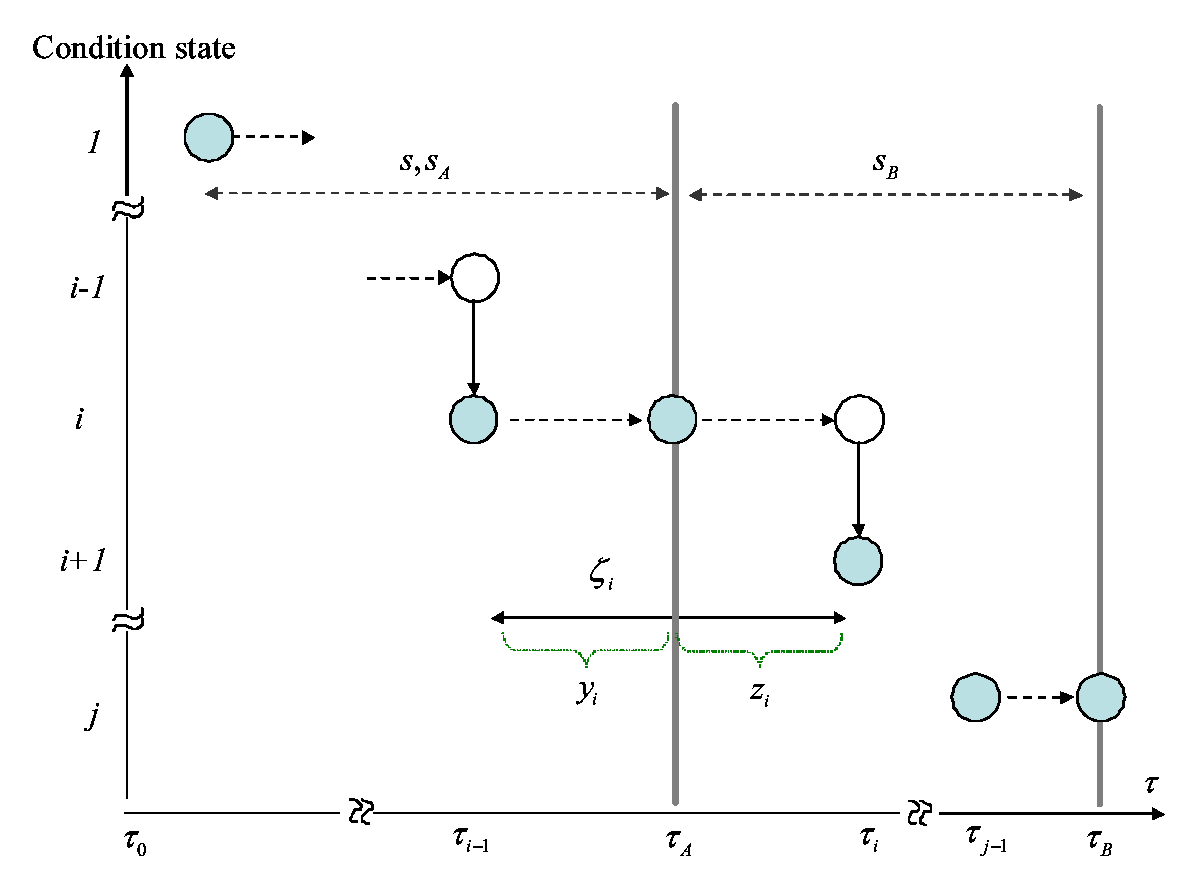
\includegraphics[scale=0.5]{fig31} 
\end{center}
\footnotesize Note) In the figure, the initial time is $\tau_0$. Condition state $i$ is observed at time $\tau_A$. For two inspection times $\tau_A$ and $\tau_B$, we represent $s_A=\tau_A-\tau_0$, $s_B=\tau_B-\tau_A$ as elapsed time. The time length $y_i$ is measured from time $\tau_{i-1}$ to time $\tau_A$, and $z_i$ is measured from time $\tau_A$ to time $\tau_i$. The total life span (survival time) of condition $i$ is expressed as $\zeta_i=y_i+z_i$.
\caption{Deterioration from Initial Time and Observation of Condition State.}
\label{fig31} 
\end{figure}%[t]
%%
\subsection{Simultaneous Occurrence Probability of Condition State at Two or More Times}
\label{333}
We assume that there are two inspection times $\tau_A$ and $\tau_B$, at which the condition states $i$ and $j$ $(i\leq j;j=1,\dots,I-1)$ are observed respectively. $\tau_{0}$ is the initial time of the deterioration process as shown in Fig. \ref{fig31}. The transition pattern of condition states occurs in the following steps. Firstly, at time $\tau_{i-1}$, condition state $i-1$ changes into condition state $i$. However, condition state $i$ can be revealed only at inspection time $\tau_A$. The duration of this event can therefore be defined as $\tau_A=\tau_{i-1}+y_i$. Secondly, at time $\tau_i=\tau_A+z_i$, the condition state advances from $i$ to $i+1$. Thirdly, condition state $i+1$ will rise to $j-1$ at time $\tau_{j-1}$. Finally, after $\tau_{j-1}$, the condition state will reach $j$ and remain in condition state $j$ until inspection time $\tau_B$. 

In Fig. \ref{fig31}, we define durations $s_A=\tau_A-\tau_0$ and $s_B=\tau_B-\tau_A$. It should be recognized from Fig. \ref{fig31} that condition state $i-1$ changes into condition state $i$ at time $\tau_{i-1}=\tau_A-y_i$. In other words, condition state $i$ is revealed at inspection time $\tau_A$;  however, it has already existed over the duration $y_i$. In addition, we define $\zeta_i$ as the life span of condition state $i$. If condition state $j$ observed at inspection $\tau_B$ is considered, the probability for this event to happen is thus dependent on the information concerning condition state $i$. Thus, by the law of conditional probability, the following conditional probability density function is defined:
\begin{eqnarray}
&& \hspace{-5mm} g_{ij}(s_B,\bar{z_i},\bar{\zeta}_{i+1},\cdots,\bar{\zeta}_{j-1}|\bar{y}_i)=\frac{f_i(\bar{y}_i+\bar{z}_i)}{\tilde{F}_i(\bar{y}_i)} \nonumber \\
&& \prod_{m=i+1}^{j-1}f_m(\bar{\zeta}_m) \tilde{F}_j(s_B-\bar{z}_i-\sum_{m=i+1}^{j-1}\bar{\zeta}_m).
\label{pt12}
\end{eqnarray}
In equation (\ref{pt12}), $y_i$ and $z_i$ are the durations measured from time $\tau_{i-1}$ to time $\tau_A$ and from time $\tau_A$ to time $\tau_i$ respectively, as shown in Fig. \ref{fig31}. The life span of condition state $i$ is defined by means of variable $\zeta_i=y_i+z_i$. Variables $z_i~(\geq 0),\zeta_{i+1}~(\geq 0),$ $\cdots,\zeta_{j-1}~(\geq 0)$ are random variables with their values to satisfy the following equation:
\begin{eqnarray}
&& 0\leq z_i+\sum_{m=i+1}^{j-1} \zeta_m < s_B.
\end{eqnarray}
Given the elapsed time $y_i$ and condition state $i$ observed at inspection time $\tau_A$, we define the conditional probability $\kappa_{ij} (s_B|y_i)$, to which condition state $j$ is observed at inspection time $\tau_B=\tau_A+s_B$:
\begin{eqnarray}
\hspace{-3mm} \kappa_{ij}(s_B|\bar{y}_i)=\int_0^{s_B}\int_0^{s_B-z_i} \cdots \int_{0}^{s_B-z_i-\sum_{m=i+1}^{j-2}\zeta_m} \nonumber \\
\hspace{2mm} g_{ij}(s_B,z_i,\zeta_{i+1},\cdots,\zeta_{j-1}|\bar{y}_i)dz_i d\zeta_{i+1}\cdots d\zeta_{j-1}.
\end{eqnarray}
Condition state $i$ can appear at any arbitrary time from the initial time to inspection time $\tau_A$. The duration $y_i$ therefore has a range in the domain $0\leq y_i\leq s_A$. Eventually, we can define the probability density $\eta_{i} (s_A,y_i)$, which describes the probabilistic relation of condition state $i$ occurring at time $\tau_{i-1} = \tau_A-y_i$:
\begin{eqnarray}
&& \eta_{i}(s_A,y_i)=\Bigg\{\int_0^{s_A-y_i} \int_0^{s_A-y_i-\zeta_1}\cdots \nonumber \\
&& \hspace{9mm} \int_0^{s_A-y_i-\sum_{m^\prime=1}^{i-3}\zeta_{m^\prime}}
\prod_{m^\prime=1}^{i-1} f_{m^\prime}(\zeta_{m^\prime}) 
 d\zeta_1\cdots d\zeta_{i-2}\Bigg\} \tilde{F}_i(y_i), \\
&& \zeta_{i-1}=s_A-y_i-\sum_{m^\prime=1}^{i-2}\zeta_{m^\prime}. \nonumber
\end{eqnarray}
As a sequel, we are able to define the explicit form for transition probability $\pi_{ij}(s_A,s_B)$, which expresses the conditional probability for condition state $i$ being observed at $\tau_A$ and condition state $j$ being observed at $\tau_B=\tau_0+s_A+s_B$:
\begin{eqnarray}
&& \hspace{-18mm}\pi_{ij}(s_A,s_B)=\mbox{Prob}[h(s_A)=i,h(s_A+s_B)=j] 
 =\int_{0}^{s_A}\eta_{i}(s_A,y_i)\kappa_{ij}(s_B|y_i)dy_i. \label{dousyutu3} 
\end{eqnarray}
The probability that condition state $I$ is observed at inspection time $\tau_A$ can be seen in  equation (\ref{oo}). If at inspection $\tau_B$, condition state $I$ is revealed, we can define the following transition probability:
\begin{eqnarray}
&& \pi_{iI}(s_A,s_B)=\pi_i(s_A)-\sum_{j=i}^{I-1}\pi_{ij}(s_A,s_B).\label{dousyutu4}
\end{eqnarray}
\subsection{Management Indicators for Infrastructure Management}
\label{334}
The life expectancy of condition state $i$ is an important indicator for infrastructure management. Life expectancy is viewed as duration, in which condition state $i$ remains until entering condition state $i+1$. In other words, life expectancy of condition state $i$ is the remaining duration counted from initial time until time $\tau_i$, at which, condition state $i$ changes to condition state $i+1$. Probabilistically, life expectancy of condition state $i$ can be expressed by means of the survival probability function $\tilde{F}_i(y_i)$ \cite{lancaster90}:
\begin{eqnarray}
&& RMD(i)= \int^{\infty}_{0}\tilde{F}_i(y_i)dy_i. \label{173}
\end{eqnarray}
The abbreviation $RMD$ stands for ``Remaining Duration''. Based on equation (\ref{prop-bFla}), we have the following equation:
\begin{eqnarray}
&& RMD(i)= \int^{\infty}_{0}\exp (-\theta_i y_i^{\alpha_i}) dy_i. \label{rating3}
\end{eqnarray}
Management indicator $RMD(i)$ is estimated based on the assumption that at time $\tau_{i-1}$ condition state changes from $i-1$ to $i$, as shown in Fig. \ref{fig31}. This calculation seems to have the  limitation that it does not capture the historical duration measured from initial time. Thus, it is necessary to define the life expectancy of condition state $i$ based on the initial time. We denote $RL(i)$, standing for ``Remaining Life'', as a management indicator, which indicates the duration of condition state $i$ counted from initial time. As can be seen from Fig. \ref{fig31}, $RL(i)$ is actually measured from time $\tau_0$ to time $\tau_i$. Given the total duration $s$ for condition state $i$ to  remain until reaching condition state $i+1$, we can define the probability density $\rho_{i}(s)$ for condition state $i$ ending its service life at time $\tau=\tau_0+s$:
\vspace{1mm}
\begin{eqnarray}
\rho_{i}(s)= \int_0^s \int_0^{s-\zeta_1} \cdots \int_{0}^{s-\sum_{m=1}^{i-2} \zeta_m} 
 \prod_{m=1}^{i-1} f_{m}(\zeta_m) f_i(s-\sum_{m=1}^{i-1} \zeta_m)d\zeta_1\cdots d\zeta_{i-1}.
\end{eqnarray}
$RL(i)$ is the expected period until the ending of condition state $i$ counted from initial time, and thus can be further defined:
\begin{eqnarray}
&& RL(i)=\int_{0}^\infty s \rho_i(s) ds. \label{r1}
\end{eqnarray}
It is noted that $RMD$ and $RL$ are fundamentally estimated based on two different assumptions of starting time. Thus, there exists a high possibility that the estimation results of these two management indicators are different. In addition to management indicators $RMD(i)$ and $RL(i)$, there is a need to estimate the life expectancy of condition state $j$ as well. As a matter of fact, the event condition state $j$ appears conditionally dependent on condition state $i$, which seems to be observed at inspection time $\tau_A$. By the law of conditional probability, we can define the conditional probability density $\nu_{j}(s|h(s_A)=i)$, at which condition state will disappear given the visual observed condition state $i$ at time $\tau_A=\tau_0+s_A$ and the elapsed duration time $s$:
\begin{eqnarray}
&& \hspace{-2mm} \nu_{j}(s|h(s_A)=i) = \frac{M*N}{\pi_i(s_A)}, \label{eq30}
\end{eqnarray}
where,
\begin{eqnarray}
&& M = \int_{0}^{s_A}
\int_0^{s_A-y_i} \int_0^{s_A-y_i-\zeta_1}\cdots \int_0^{s_A-y_i-\sum_{m^\prime=1}^{i-3}\zeta_{m^\prime}}f_i(y_i+z_i)\cdot \nonumber\\
&& \hspace{80mm}\prod_{m^\prime=1}^{i-1} f_{m^\prime}(\zeta_{m^\prime})dy_i d\zeta_1\cdots d\zeta_{i-2}dz_i, \nonumber \\
&& N = \int_0^{s}\int_0^{s-z_i} \cdots \int_{0}^{s-z_i-\sum_{m=i+1}^{j-2}\zeta_m }\prod_{m=i+1}^{j-1}f_m(\zeta_m)  \nonumber \\
&& \hspace{75mm}f_j(s-z_i-\sum_{m=i+1}^{j-1} \zeta_m)d\zeta_{i+1}\cdots  d\zeta_{j-1}, \nonumber \\
&& (i\leq j; j=1,\cdots,I-1) \hspace{3mm} \text{and} \hspace{3mm} \zeta_{i-1}=s_A-y_i-\sum_{m^\prime=1}^{i-2}\zeta_{m^\prime}. \nonumber
\end{eqnarray}
The denominator of equation (\ref{eq30}) refers to deterioration state probability for condition state $i$, which remains until time $s_A$. In the numberator, $M$ represents the event that condition state $i$ remains until increment time $z_i$, and  $N$ represents the event that condition state $i$ changes to $j$ at elapsed time $\zeta_{j-1}$ and stays up to duration $s$. Eventually, we define the life expectancy of condition state $j$ ($j \geq i$) as $RL_{j}(h(s_A)=i)$, which conditionally depends on condition state $i$ with duration $s_A$:
%%%%%%%%%55
\begin{eqnarray}
&&\hspace{-3mm}  RL_{j}(h(s_A)=i)=\int_{0}^{\infty} s \nu_j(s|h(s_A)=i)ds,
\label{r2}\\
&& (i\leq j; i,j=1,\cdots,I-1). \nonumber
\end{eqnarray}
%%%
\section{Estimation Method}
\label{34}
\subsection{Content of Data from Visual Inspection}
\label{341}
Suppose visual inspection data on the same kind of $K$ infrastructure components is available. An inspection sample $k~(k=1,\cdots,K)$ describes two visual inspection times carried out at initial time $\bar{\tau}_0^k$ and $\bar{\tau}_A^k$ with the concerning condition state $h(\bar{s}^k)$. The symbol $\lfloor\bar{\text{    }}\rceil$ indicates an actual measurement. $\bar{s} ^k=\bar{\tau} _ A^k-\bar{\tau} _ 0^k$ is the duration between two inspection times. In addition, a dummy variable $\bar{\mbox{\boldmath$\delta$}}^k=\{\bar{\delta}_{i}^k~(i=1,\cdots,I)\}$ based on the deterioration progress patterns between two inspection times is defined as
\begin{eqnarray}
&& \bar{\delta}_{i}^k=\left\{
\begin{array}{ll}
1 & h(\bar{s}^k)= i\\
0 & \text{Otherwise}
\end{array}.
\right.
\end{eqnarray}
Furthermore, in order to describe the information in sample $k$, we use characteristic vector  $\bar{\mbox{\boldmath$x$}}^k=(\bar{x}_1^k,\cdots,\bar{x}_N^k)$ and elapsed duration $\bar{s}^k$.  $\bar{x}_n^k~(n=1,\cdots,N)$ represents the value of a characteristic variable $n$ visually observed in the sample $k$. Thus, the information contained in inspection sample $k$ can be rearranged as  $\bar{\xi^k}=(\bar{\mbox{\boldmath$\delta$}}^k,\bar{s}^k,\bar{\mbox{\boldmath$x$}}^k)$. As a result, we can further express the Weibull hazard function for sample $k$ as
%%
%%
\begin{eqnarray}
&& \lambda_i^k(y_i)=\theta_i^k \alpha_{i} y_i^{\alpha_{i}-1} ~(i=1,\cdots,I-1). \label{pt26}
\end{eqnarray}
It is noted that the hazard function is not defined for condition state $I$ since $I$ is absorbing state and $\mathop{\lim}\limits_{s\to\infty}\pi_I(s) = 1$. As a matter of course, the value of hazard rate $\theta_i^k~(i=1,\cdots,I-1;k=1,\cdots,K)$ changes according to the property of characteristic vectors of sample $k$. The dependency of hazard rate on characteristic vector $\bar{\mbox{\boldmath$x$}}^k$ can be formulated by means of functional relationship as
\begin{eqnarray}
&&
\theta_i^k=\bar{\mbox{\boldmath$x$}}^k\mbox{\boldmath$\beta$}_i^\prime\label{hazard13}
\end{eqnarray}
where $\mbox{\boldmath$\beta$}_i=(\beta_{i1},\cdots,\beta_{iN})$ is a row vector of unknown parameter $\beta_{in}~(n=1,\cdots,N)$, and the symbol $\prime$ indicates that the vector is transposed. The functional relationship between hazard rate and characteristic variable can be changed according to  preferences in estimation. This issue can be further viewed in the relationship assumption in our empirical study.

Later in this section, the methodology to estimate the transition probability will be presented. At first, based on the Weibull hazard function $\lambda_i^k(y_i)$ with collected sample information $\bar{\xi^k}~(k=1,\cdots,K)$, the likelihood function for transition probability is defined. Based on the maximum likelihood estimation approach, we can obtain the values for unknown parameters in equation (\ref{hazard13}) and further for the parameterized values of the Weibull hazard function. Secondly, the estimation method is proposed for the transition probability when there are two or more than two inspection data. Finally, we explain the necessity of estimating the expected deterioration probability as a representative value when there is a large pool of sampling data.
%%%%%%
\subsection{Estimate of Weibull Hazard Function}
\label{342}
As earlier mentioned, data concerning inspection sample $k$ can be rearranged as $\bar{\xi^k}=(\bar{\mbox{\boldmath$\delta$}}^k,\bar{s}^k,\bar{\mbox{\boldmath$x$}}^k)$. The application of the Weibull hazard function in estimating the deterioration state probability is discussed in equations  (\ref{ii1}),(\ref{i2}),(\ref{dousyutu1}),(\ref{oo}). Applying the characteristic vector $\bar{\mbox{\boldmath$x$}}^k$ of infrastructure component, we can calculate the hazard rate expressed in equation (\ref{hazard13}). Moreover, the deterioration state probability depends on the duration of operation $\bar{s}^k$ after the opening time of the infrastructure. Therefore, in order to express clearly this characteristic, the deterioration state probability $\pi_{i}(\bar{s}^k)$ can be defined as a function of measured visual inspection data $(\bar{s}^k,\bar{\mbox{\boldmath$x$}}^k)$ and unknown parameter vector $\mbox{\boldmath$\gamma$}=\{\mbox{\boldmath$\alpha$},\mbox{\boldmath$\beta$}_i~(i=1,\cdots,I-1)\}$. $\mbox{\boldmath$\alpha$}=(\alpha_{1},\cdots,\alpha_{I-1})$ is a row vector of unknown parameter $\alpha_{i}~(i=1,\cdots,I-1)$. 

If the deterioration progress of the infrastructure components in  $K$ samples are assumed to be mutually independent, the log-likelihood function expressing the simultaneous probability density of the deterioration transition pattern for all inspection samples is  
\begin{eqnarray}
&& \hspace{-10mm} \ln[{\cal L}(\mbox{\boldmath$\gamma$})] = \ln
\left[\prod_{i=1}^{I} \prod_{k=1}^{K}
\left\{\pi_{i}(\bar{s}^k,\bar{\mbox{\boldmath$x$}}^k:\mbox{\boldmath$\gamma$})\right\}^{\bar{\delta}_{i}^k}\right]
%\nonumber \\
 =\sum_{i=1}^I \sum_{k=1}^{K} \bar{\delta}_{i}^k
\ln\left[
\pi_{i}(\bar{s}^k,\bar{\mbox{\boldmath$x$}}^k:\mbox{\boldmath$\gamma$})\right],
\label{logbF3}
\end{eqnarray}
where $\bar{\mbox{\boldmath$\delta$}}^k$, $\bar{s}^k$, $\bar{\mbox{\boldmath$x$}}^k$ are all determined through inspection and $\mbox{\boldmath$\gamma$}$ is a parameter to be estimated \cite{tobin,amemi}. Estimation of parameter  $\mbox{\boldmath$\gamma$}$, given an amount of $\hat{\mbox{\boldmath$\gamma$}}=(\hat{\gamma}_{10},\cdots,\hat{\gamma}_{I-1N})$, can be obtained by solving the optimality conditions
\begin{eqnarray}
&& \frac{ \partial \ln[{\cal L}(\hat{\mbox{\boldmath$\gamma$}})] }{\partial
\gamma_{in}}=0, \quad ~(i=1,\cdots,I-1;n=0,1,\cdots,N), \label{saiteki3}
\end{eqnarray}
that result from maximizing the log-likelihood function (\ref{logbF3}). The optimal values $\hat{\alpha}_i=\hat{\gamma}_{i0}$ and $\hat{\mbox{\boldmath$\beta$}}_i=(\hat{\gamma}_{i1},\cdots,\hat{\gamma}_{iN})$ are then estimated by applying a numerical iterative procedure such as the Newton method for the $(I-1)\times (N+1)$ order nonlinear simultaneous equations \cite{tuma}. Moreover, estimator for the asymptotical covariance matrix of the parameters ($\hat{\mbox{\boldmath$\Sigma$}}(\hat{\mbox{\boldmath$\gamma$}})$) is given by
\begin{eqnarray}
&& \hat{\mbox{\boldmath$\Sigma$}}( \hat{\mbox{\boldmath$\gamma$}})
= \left[ \frac{ \partial^2\ln\{ {\cal L}( \hat{\mbox{\boldmath$\gamma$}})\}
}{\partial \mbox{\boldmath$\gamma$} \partial \mbox{\boldmath$\gamma$}'}
\right]^{-1}.
\end{eqnarray}
The $(I-1)(N+1)\times (I-1)(N+1)$ order invert matrix of the right-hand side of the above equation, composed of the element $\partial^2\ln\{{\cal L}(\hat{\mbox{\boldmath$\gamma$}})\}/\partial \gamma_{in} \partial \gamma_{i^\prime n^\prime}$ results in the invert matrix of the Fisher information matrix \cite{greene}. In the above-mentioned calculation process, it might not be necessary directly to estimate the deterioration state probability $\pi_i(s)$ from the log-likelihood function of equation (\ref{logbF3}). The deterioration state probability can be estimated from multiple integration of equation (\ref{dousyutu1}). Suffice it to say that the accuracy of estimation for  $\hat{\mbox{\boldmath$\gamma$}}$ depends on the accuracy in calculating the multiple integration. Considering this challenge, in this research we employ double integration, suggested by \citet{steven98}, to improve the accuracy of multiple integral calculation.
%%%%%%%%%
\subsection{Estimation Method for the Case of Having Data from Two or More Visual Inspections}
\label{343}
In general management practice, the database is composed only of data from two inspection times. However, future monitoring activities may be expanded so as to provide the advantage of data for more than two inspection times. Therefore, besides the estimation methodology for two inspection times as earlier discussed, it is necessary to develop a method to take multi-inspection times into account.

For sample $k$, we assume the condition states $h(\bar{s}_A^k)$ and $h(\bar{s}_A^k+\bar{s}_B^k)$ are respectively observed at inspection times $\bar{\tau}_A^k$ and $\bar{\tau}_B^k$. $\bar{\tau}_0^k$ is defined as initial time. Thus, two durations of operation according to two inspection times are further defined as $\bar{s}_A^k=\bar{\tau}_A^k-\bar{\tau}_0^k$ and $\bar{s}_B^k=\bar{\tau}_B^k-\bar{\tau}_A^k$. Additionally, a dummy variable $\mbox{\boldmath$\bar{\Delta}$}^k=\{ \bar{\delta}_{ij}^k~(i=1,\cdots,I-1, j=1,\cdots,I)\}$ is determined based on the transition pattern observed from inspections:
%
\begin{eqnarray}
&& \bar{\delta}_{ij}^k=\left\{
\begin{array}{ll}
1 & h(\bar{s}_A^k)=i,h(\bar{s}_{A}^k+\bar{s}_B^k)= j\\
0 & Otherwise
\end{array}.
\right.
\end{eqnarray}
The information of inspection sample $k$ can be rearranged as $\Xi^k=(\bar{\mbox{\boldmath$\Delta$}}^k,\bar{\mbox{\boldmath$s$}}^k,\bar{\mbox{\boldmath$x$}}^k)$. Since the duration $\bar{\mbox{\boldmath$s$}}^k=(\bar{s}_A^k,\bar{s}_B^k)$ is observable, the deterioration state probability can be estimated according to equations (\ref{dousyutu3}) and (\ref{dousyutu4}). Precisely, the transition probability $\pi_{ij}(\bar{s}_A^k,\bar{s}_B^k)$ can be expressed by means of the function of $\pi_{ij}(\bar{\mbox{\boldmath$s$}}^k,\bar{\mbox{\boldmath$x$}}^k:\mbox{\boldmath$\gamma$})$, in which  the data $(\bar{\mbox{\boldmath$s$}}^k,\bar{\mbox{\boldmath$x$}}^k)$ are available from visual inspections, thus making unknown parameter $\mbox{\boldmath$\gamma$}$ the only target of estimation. The description of unknown parameter $\mbox{\boldmath$\gamma$}=\{\mbox{\boldmath$\alpha$},\mbox{\boldmath$\beta$}_i~(i=1,\cdots,I-1)\}$ is similar to that explained earlier in this section.

In a similar approach to equation (\ref{logbF}), we define the log-likelihood function for transition probability as follows:
\begin{eqnarray}
&& \hspace{-3mm} \ln[{\cal L}(\mbox{\boldmath$\gamma$})] = \ln
\left[\prod_{i=1}^{I-1}\prod_{j=i}^{I} \prod_{k=1}^{K}
\left\{\pi_{ij}(\bar{\mbox{\boldmath$s$}}^k,\bar{\mbox{\boldmath$x$}}^k:\mbox{\boldmath$\gamma$})\right\}^{\bar{\delta}_{ij}^k}\right]
\nonumber \\
&& \hspace{5mm} = \sum_{i=1}^{I-1} \sum_{j=i}^I \sum_{k=1}^{K}\bar{\delta}_{ij}^k
\ln\left[
\pi_{ij}(\bar{\mbox{\boldmath$s$}}^k,\bar{\mbox{\boldmath$x$}}^k:\mbox{\boldmath$\gamma$})\right].
\label{lsogbF}
\end{eqnarray}
By applying the maximum likelihood estimation approach, we can obtain the value for unknown parameter $\hat{\mbox{\boldmath$\gamma$}}$. We will omit a detailed explanation, since this is similar to a reference mentioned earlier in this section. Nevertheless, it is worth emphasizing that the case when $i=I$ is not embedded in the degree of equation (\ref{lsogbF}) since $I$ is the absorbing state.
%%%
\subsection{Expected Deterioration State Probability}
\label{344}
The research methodology for deterioration estimation can be applied to every individual infrastructure component. However, in practice, when the deterioration pattern of a large amount of sampling data is considered, it is more convenient to estimate the expected deterioration state probability rather than to focus on that of individual components. 

With regard to the relationship between the hazard rate $\theta_i^k~(k=1,\cdots,K)$ of sample $k$ and the characteristic variable $x$, it is understandable to express the distribution function of characteristic variable as $\Gamma(\mbox{\boldmath$x$})$. Thus, statistically, the expected value of the hazard rate $E [\theta_i]$ can be defined by means of the distribution function of characteristic variable $x$:
\begin{eqnarray}
&& E[\theta_i]=\int_{\Theta}\mbox{\boldmath$x$}\mbox{\boldmath$\beta$}_i^\prime d\Gamma(\mbox{\boldmath$x$}),\label{oiu3}
\end{eqnarray}
where $\Theta$ refers to the entire sample population. After averaging the value of the hazard rate, we can again define the Weibull hazard function as
\begin{eqnarray}
&& \overline{\lambda}_i(y_i)=E[\theta_i] \alpha_{i} y_i^{\alpha_{i}-1}. \label{hazardg}
\end{eqnarray}
Eventually, after the expected hazard rate is estimated from equation (\ref{hazardg}), the expected deterioration state probability (equations (\ref{ii1}), (\ref{i2}), (\ref{dousyutu1}) and  (\ref{oo})) and the life expectancy of condition states (equations (\ref{r1}) and (\ref{r2})) can be obtained. 
\section{Empirical Study}
\label{35}
\subsection{Overview of Empirical Study}
\label{351}
In this section, we present an empirical application to further verify the applicability of the model, using visual inspection data on the tunnel lighting system of northeast branch office of the Japan Public Highway Corporation. Visual inspection was conducted to record the condition of steel board and stainless steel plate (SUS), the two main materials used in the lighting system. However, due to the lack of sufficient data on SUS, only results from the visual observation of steel board are used as an application experience. Data concerning the structural visual inspection of tunnel lighting were collected between April 2002 and January 2003. The database also contains information from the opening  date. Average duration from the starting of operation to visual inspection is about 11.8 years. The condition states are ranked by a rating of $OK$, $B$, $A$, and $AA$, explained in detail in Table \ref{table31}.

%%%
\begin{table}[t]
\begin{center}
\caption{Deterioration Rank Criterion.}
\label{table31}
{\footnotesize
\begin{tabular}{c|c|p{6cm}}
Inspection result & Condition state & Physical description \\\hline
OK & 1 & There is no damage.\\
B & 2 &The depression is not seen though there is damage.\\
 &  & The progress of the damage is observed.\\
A & 3 &  There is damage, the depression is seen, and the repair is carried out.\\
 &  &    Urgent repair is not required.\\
AA & 4 & Damage is obvious and urgent repair is required to enable functioning.\\\hline
\end{tabular}
}
\end{center}
\end{table}

%%%
In total, we used $12,311$ sample data from the database for empirical analysis. From among the sample data, the transition of deterioration ranks in regard to visual inspection times are rearranged in Table \ref{table32}. The average duration of operation counted from the staring time of the infrastructure is also shown in the table. The deterioration pattern is reflected by the transition of deterioration condition states being observed at respective visual inspection times. If the deterioration progress of a lighting facility advances to condition state $AA$, repair is carried out. The recorded data also show the classification at the time when visual inspection is carried out. For example, in the total amount of $10,238$ samples in condition state $A$ at visual inspection time (group of transition pattern from $OK \rightarrow A$), there are $6,073$ samples in the group of those without historical repair, 4,165 samples having already received repair in the past. Visual inspection also reveals 750 samples reaching condition state $AA$, which required immediate repair. Consequently, the total numbers of samples receiving repair action became  $4,165+750=4,915$ in the end, and the average operation duration of those facilities reached about $15.36$ years. 
 
\begin{table}[t]
\caption{Number of Sample Data.}
\label{table32}
{\small
\begin{center}
\begin{tabular}{c|c|c}
 & Number of samples & Average operation duration \\\hline
OK $\rightarrow$ OK & 2 & 5.24 years \\\hline
OK $\rightarrow$ B & 1,321 & 8.31 years \\\hline
OK $\rightarrow$ A & 10,238  & 11.98 years \\\cline{2-3}
(no historical repair) & 6,073 & 9.72 years \\\hline
OK $\rightarrow$ AA & 750 & 15.91 years \\\cline{2-3}
(After repair) & 4,915 & 15.36 years \\\hline
Total & 12,311 & \\\hline
\end{tabular}
\end{center}
}
\end{table}%[t]
%%%%%%%%
\subsection{Hazard Model Estimation}
\label{352}
As for physical characteristics, at first, four variables are reviewed as potential candidates,  including elapsed time $\bar{s} ^k$, type of lighting facility (normal lighting and eased lighting), traffic volume and tunnel inclination. The purpose of combining explanatory variables is to maximize the aforementioned log-likelihood function with a significant level of $t-$ values. Finally, we selected elapsed time and type of lighting as explanatory variables. In addition, we defined the Weibull hazard function as a function of variables as follows:
\begin{eqnarray}
\lambda_i^k(y_i^k)=\alpha_{i}(\beta_{i0}+\beta_{i1}d^k) (y_i^k)^{\alpha_{i}-1} ~(i=1,2,3).
\label{pt335}
\end{eqnarray}
In equation (\ref{pt335}), a dummy variable $d^k$ is added. Its value is defined based on the type of lighting facility. For example, $d^k=0$ is for the case when sample $k$ is a normal lighting facility; otherwise, $d^k=1$. Variable $y_i^k$ indicates the elapsed time over which sample $k$ stays in condition state $i$. It is noted that variable $y_i^k$ cannot be observed directly. Thus, when we detect $\bar{i}$ as the condition state of sample $k$, we define the summation of duration as $\sum_{m=1}^{\bar{i}} y_m^k=\bar{s}^k$. 

Estimation results are presented in Table \ref{table33}. It can be seen from the table that there is a significant difference between types of lighting facilities. The values of the unknown parameter and its statistical $t-value$ associated with the type of lighting facility receives its negative value for condition state $1$. After verification, we recognized the fact that eased lighting, which is located at the tunnel opening, has an early deterioration speed. Thus, the estimation results corresponded exactly to the observed information. Regarding the deterioration of condition states $2$ and $3$, estimation results proved that type of lighting facility does not have a significant impact.

Table \ref{table33} further displays comparative results between the Multi-stage Weibull hazard model and the Multi-state Markovian hazard model. The reason behind the comparison is that the Multi-state Markovian hazard model is in fact a special case of the Multi-stage Weibull hazard model, as when acceleration parameter $\alpha$ in the Weibull hazard function equals $1$. It is realized from the table that the acceleration in value of $\alpha$ exactly corresponds to the growth of condition states ($\alpha_1=2.039$, $\alpha_2=1.623$, and $\alpha_3=5.709$). In addition, it is concurrently found that the increase in the elapsed time is in correlation with the increase in value $\alpha$.

Fig. \ref{fig32} displays the relationship between elapsed time $y_1$ of condition state $1$ and the survival probability probability $\tilde{F}_1(y_1)$ for both normal lighting ($d^k=1$) and eased lighting ($d^k=0$). It can be seen from the figure that normal lighting has a higher probability of  surviving than the eased lighting. The life expectancy of condition state $1$ for eased lighting is relatively short. For instance, after approximately $y_1 \simeq 1.7$ years in operation, $80\%$ of the total number of eased lighting in condition state $1$ will change into condition state $2$. On the other hand, $50\%$ of the total number of normal lighting still remains in condition state 1.

Fig. \ref{fig33} shows the distribution pattern of condition states in relation to the duration of  operation time of a normal lighting facility. It is noted that after approximately $6$ years in operation, condition state $1$ will be on the verge of disappearing. Based on this finding, it is advisable to implement visual inspection after about 6 years. Moreover, as noted from table \ref{table32}, condition states $3$ and $4$ account for a large proportion of the sampling population after about $15$ years of operation. Therefore, in terms of management, it might be too risky for inspection time to be allocated around the time when there is a high possibility of the onset of condition states 3 and 4.
%%%%%%%
\subsection{Calculation of Management Indicators}
\label{353}
Table \ref{table34} presents comparative estimation results for management indicators $RMD(i)$ and $RL(i)$. It is certain that the values of $RMD(i)$ and $RL(i)$ estimated by the Multi-stage Markovian hazard model  exert only slight differences. However, a significant difference between the values of $RMD(i)$ and $RL(i)$ is realized for condition state $3$ when employing the Multi-stage Weibull hazard model ($RMD(3)=7.30$ and $RL(3)=12.95$). This result further proves the impact of elapsed time on estimation results. 

A comparision of the values of $RL(3)$ between the two models shows that the value estimated with the  Multi-stage Weibull hazard model is shorter than that estimated by using the Multi-stage Markovian hazard model ($RL(3) =16.34$). In addition, the average duration measured in Table \ref{table32} ($15.36$) is shorter than that of the Multi-stage Markovian hazard model. These differences are due to the fact that the average operation duration calculated in Table \ref{table32} and the average operation duration calculated with the multi-stage Markovian hazard model took $4,165$ samples, which had already received repair in the past. In other words, the data used for calculation in Table \ref{table32} and for the multi-stage Markovian hazard model has not been censored.

%%%
\begin{table}[t]
\begin{center}
\caption{Result of Hazard Model Estimation.}
\label{table33}
{\footnotesize
\begin{tabular}{c|c|c|c|c|c|c|c|c}
& \multicolumn{4}{|c|}{Multi-stage Weibull hazard model} & \multicolumn{4}{|c}{Multi-stage Markovian hazard model}\\\hline
Condition state & $\alpha_i$ & $\beta_{i0}$ & $\beta_{i1}$ & $E[\theta_i]$ & $\alpha_i$ &$\beta_{i0}$ & $\beta_{i1}$ & $E[\theta_i]$ \\ \hline
1 & 2.039 &0.548 & -0.323 & 0.367 & 1.0 &1.054 & -0.370 & 0.847 \\
$t$\text{ value} & (477.54) & (6.14) & (-3.49) & - & - & (10.12) & (-3.66) & - \\\hline
2 & 1.623 & 0.0812& -& 0.0812 & 1.0  & 0.265 & - & 0.265 \\
$t$\text{ value} & (469.92) & (32.90) & - & - & - & (58.99) & -& - \\\hline
3 & 5.709 & 0.000011& - & 0.000011 & 1.0 & 0.0882 &- & 0.0882 \\
$t$\text{ value} & (1486.69) & (15.10) & - & - & - & (35.43) & - & - \\\hline
Initial log-likelihood & \multicolumn{4}{|c|}{-811,804.79} & \multicolumn{4}{|c}{-811,804.79}\\
Log-likelihood & \multicolumn{4}{|c|}{-7,041.67} & \multicolumn{4}{|c}{-8,996.89}\\
Likelihood ratio & \multicolumn{4}{|c|}{0.991} & \multicolumn{4}{|c}{0.989}\\\hline
\end{tabular}
}
\end{center}
\end{table}
%%%
%%%
\begin{figure}[t]
\begin{center}
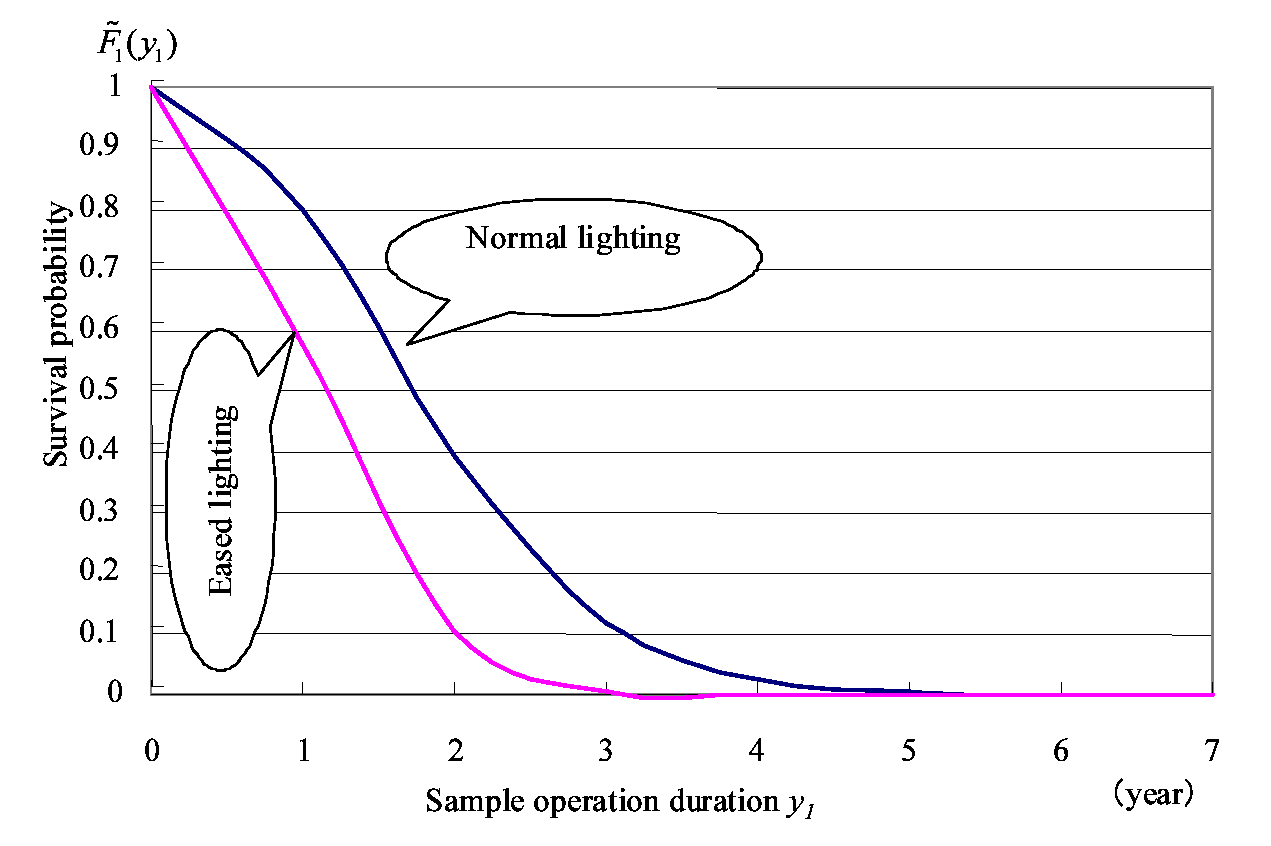
\includegraphics[scale=0.5]{fig32} 
\end{center}
\footnotesize Note) Slopes of survival probabilities $\tilde{F} _ 1(y_1) $ for condition state 1 along operation duration $y_1$ drawn for normal lighting and eased lighting.
\caption{Survival Probability $\tilde{F}_1(y_1)$.}
\label{fig32}
\end{figure}
\begin{figure}[t]
\begin{center}
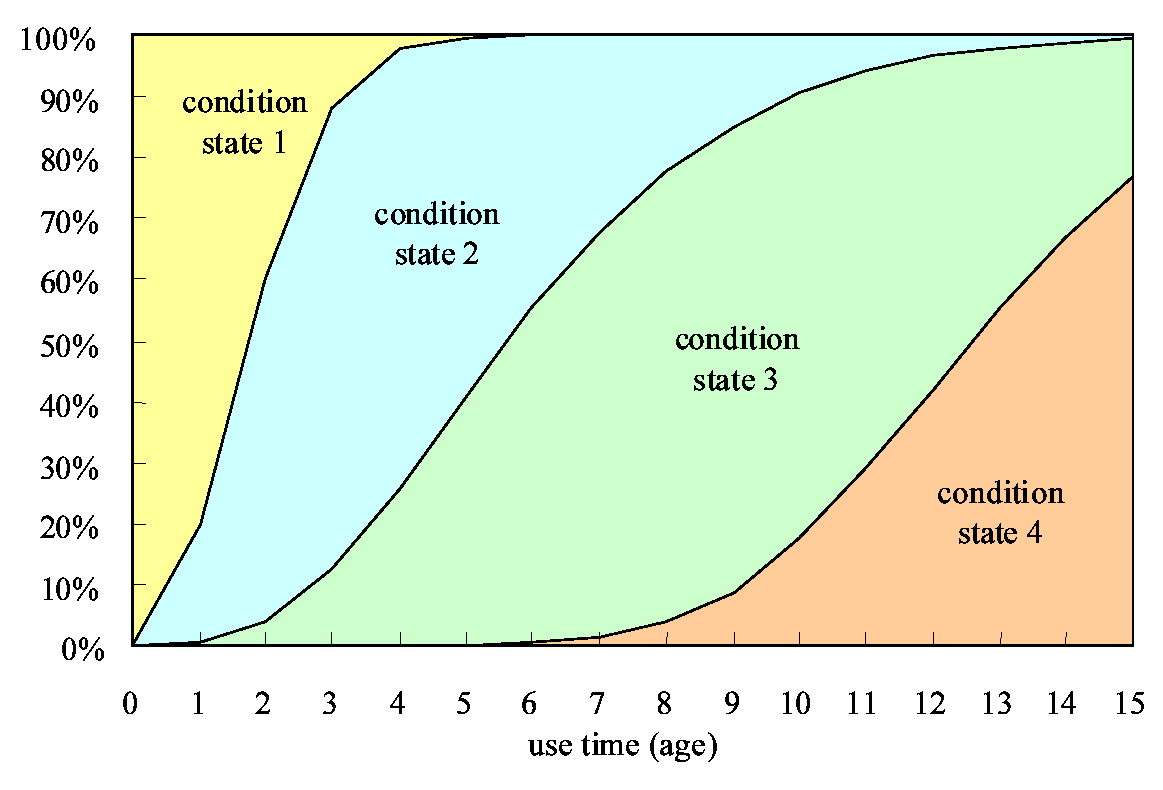
\includegraphics[scale=0.5]{fig33} 
\end{center}
\footnotesize Note) The relation between operation duration $s$ from initial time and deterioration state probability $\pi_i(s) $ for normal lighting.
\caption{Deterioration State Probability $\pi_i(s)$.}
\label{fig33}
\end{figure}
%%
%%
\begin{table}[t]
\begin{center}
\caption{Management Indicator.}
\label{table34}
{\footnotesize
\begin{tabular}{c|c|c|c|c}
 & \multicolumn{2}{|c|}{Life expectancy} & \multicolumn{2}{|c}{Initial life expectancy} \\
Condition state & \multicolumn{2}{|c|}{$RMD(i)$ years} & \multicolumn{2}{|c}{$RL(i)$ years} \\ \cline{2-5}
 & Weibull & Markov & Weibull & Markov \\\hline
1 & 1.45 & 1.23 & 1.45 & 1.27 \\
2 & 4.20 & 3.77 & 5.65 & 5.00 \\
3 & 7.30 & 11.34 & 12.95 & 16.34 \\ \hline
\end{tabular}
}
\end{center}
\footnotesize Note)  Multi-stage Weibull hazard model and multi-stage Markovian hazard model.
\end{table}
%%%
\begin{table}[t]
\begin{center}
\caption{Life Expectancy and Corresponding Condition State $RL_{3}(h(s_A)=i)$.}
\label{table35}
{\footnotesize
\begin{tabular}{c|c|c|c}
Condition state $i$ & $i=1$  & $i=2$ & $i=3$ \\ \hline
$s_A=2$ & 11.85 years & 10.54 years & 6.40 years \\
$s_A=4$ & | & 9.94 years & 5.77 years \\
$s_A=6$ & | & 9.39 years & 4.92 years \\
$s_A=8$ & | & 9.02 years & 3.96 years \\
$s_A=10$ & | & | & 3.15 years \\
$s_A=12$ & | & | & 2.60 years \\ \hline
\end{tabular}
}
\end{center}
\footnotesize Note)  Only elapsed time $s_A$, which displays only the case of survival probability more than 10\%.
\end{table}

Finally, the estimation results for management indicator $RL_{3} (h(s_A)=i) $ are shown in Table \ref{table35}, where values of $RL_{3} (h(s_A)=i) $ are presented  corresponding to the elapsed time $s_A$ and condition state $i$. The values presented in the last column of the table highlights the fact that when elapsed time increases, the life expectancy of condition states tends to decrease.
\section{Summary and Recommendations}
\label{36}
This chapter has presented an analytical methodology using the multi-stage Weibull hazard model for forecasting the deterioration process of infrastructure facilities. The deterioration process is represented by a transition pattern among multiple condition states. In the estimation approach, the maximum likelihood method is employed to estimate the parameters of the model based on observed condition states, characteristic variables and elapsed time of disaggregate samples collected through  inspections.

The proposed model makes it possible to estimate the transition probability of condition states for any arbitrary time intervals. In order to verify the applicability of the model, an empirical study was conducted on a database of tunnel lighting facilities of express highways in Japan. This study has made a contribution to the field by benchmarking findings  with estimation results using the Multi-stage Markovian hazard model. The analytical methodology presented can be extended to apply not only to tunnel lighting facilities but to various other kinds of infrastructure facilities as well.

However, we have not discussed several points, which will be considered as topics for extending this study in the future:
\begin{itemize}
 \item Measurement errors occurring in monitoring and inspection activities have not been addressed in this model. In order to tackle this problem, for example, a methodology using Bayesian estimation and Markov Chain Monte Carlo, for example, can be incorporated into the model in the future.
 \item The samples used in empirical study shared almost similar structural characteristics. However, in general practice, an infrastructure database system is often comprised of heterogeneous groups. Thus, the impacts of individual groups on the overall deterioration process should be investigated. A methodology using the mixture mechanism in hazard analysis can be proposed for future consideration.
 \item In future management, a tendency might develop whereby shorter inspections will become common due to innovations in technology. Hence, the database system of infrastructure management should be designed in such a way that it can be synchronized with an analytical frame. As a sequel, the future focus on multi-schemes inspection data should be considered.
\end{itemize} % Multi-stage Weibull Hazard Model on Tunnel Lighting System

% Chapter 3

\chapter{A Hidden Markov Deterioration Model with Measurement Errors} % Write in your own chapter title
\label{Chapter4}
\lhead{Chapter 4. \emph{A Hidden Markov Deterioration Model with Measurement Errors}} % Write in your own chapter title to set the page header

\section{General introduction}
\label{41}
%The Markov chain model has been widely documented as an important methodology in hazard analysis of infrastructure asset management \cite{madanat95,shin,shahin05}. A good example of its application can be referred to PONTIS program, which was developed for bridge management \cite{pontis}. Fundamentally, Markov chain model is applied for forecasting the deterioration process, performance of infrastructure over time. In the model, discrete states are classified to represent the performance condition of infrastructure. The deterioration, as transition pattern among states, is simulated as stochastic process based on theory of Markov chain. 
%
Application of Markov hazard models requires monitoring data from at least two inspection times. Thus, the accuracy of estimation largely depends on the quality of monitoring data. Errors exist in monitoring data are referred as measurement errors arising from measurement system or inspector (human or machine), inspected objects, or from data processing and data interpretation \cite{humplick}. Measurement errors tend to cause  estimation results to be different from what they should be, especially under a small pool of monitoring data.

This chapter proposes a hidden Markov deterioration model, with an innovative analytical method to eliminate the negative influence of measurement errors on estimation results. In the model, measurement errors are assumed as random variables. In addition, the functional relation between the ``true condition states'' and ``measurement errors'' of an infrastructure component is formulated by a mixture mechanism. Precisely, the mixing mechanism is referred as the dispersion of the ``observed condition states'' to the ``true condition states''. To estimate the parameters of the model, we apply the method of maximum likelihood, together with the  Bayesian estimation and MCMC simulation.

The following section presents a framework on measurement errors and the process of deterioration with hidden condition states. Section \ref{44} details the mathematical formulation of mixture distribution and hidden Markov transition probability. An analytical technique using Bayesian estimation and MCMC simulation is discussed in section \ref{45}. Section \ref{46} illustrates an empirical study using data of Japanese national road system. The last section summarizes contributions of the model and further includes a discussion for future research.
%%%%%%%%%%%%%%%%%%%%%%%%%%
\section{Measurement errors and hidden condition states}
\label{42}
\subsection{Measurement errors and the problem of representative values}
\label{421}
In infrastructure management practices, the healthy status or performance of an infrastructure component is described in discrete condition states, which are defined by means of a single performance index or an aggregate index. The values of indexes are measured by monitoring and visual inspection. For example, in the case of pavement management system (PMS), the condition states include the extend of several pavement distress such as rut and cracking, or some aggregate condition states, such as the Pavement Condition Index (PCI) \cite{shahin05}.

However, because of measurement errors, the true condition states may not be captured. Fig. \ref{fig41} presents a problem of having measurement errors in the PMS. The values on both horizontal and vertical axes indicate the rut index, which are measured at inspection time $\tau_A$ and $\tau_B~(\tau_A<\tau_B)$ respectively. If there is no maintenance and repair ($M\&R$) actions during the past inspection period ($6$ years), the dots representing the values of ruts should be located above the $45^o$ line. However, as can be seen from the figure, a great numbers of dots are  located under the $45^o$ line, inferring measurement errors. As a result, the observed condition states representing by the dots under the $45^o$ line might be used in the hazard analysis instead of using the true condition states. The problem of representation of condition states is referred as the ``representation matter''.

%%%
\begin{figure}
\begin{center}
\begin{footnotesize}
\includegraphics[scale=0.5]{fig41.eps}\\
Note) Samples under the $45^0$ line represent the values of the rut index for road sections. \\
\caption{Measurement errors in pavement management system.}
\label{fig41}
\end{footnotesize}
\end{center}
\end{figure}
%%%%%%%
\subsection{The process of deterioration in hidden Markov hazard model} \label{422}
A clear picture of measurement errors can be seen from Fig. \ref{fig42}. In the figure, the  deterioration of a road section is described as the transition pattern among condition states $i$ $(i=1,...,I)$, with $i=1$ as the new condition state and $i=I$ as the worst condition state (absorbing condition state). Two visual inspections are supposed to be carried at inspection times $\tau_A$ and $\tau_B$. In addition, there is no $M\&R$ action during the interval $[\tau_A$, $\tau_B]$. The observed condition state of the road section at inspection times $\tau_A$ and $\tau_B$ are $m(\tau_A)=m(m=1,...,I)$ and $n(\tau_A)=n(n=1,...,I) (m \leq n)$ respectively. However, because of measurement errors, the observed condition state is different from the true condition state, which is supposed to be equal to  $m^\ast(\tau_A)=i~(i=1,\cdots,I)$ at times $\tau_A$ and $m^\ast(\tau_B)=j~(j=1,\cdots,I)$ at times $\tau_B$.

In monitoring practices, to quantify the condition state of a road section, several values of distress are examined. However, inspectors tend to select the worst condition state  among the observed condition states of distress to be the representative condition state of that section. As can be seen from the Fig. \ref{fig42}, the ``true condition state'' $m^\ast(\tau_A)=i$ at times $\tau_A$ is lower than the ``observed condition state'' $m(\tau_A)=m$ at times $\tau_B$. 

\begin{figure}
\begin{center}
\begin{footnotesize}
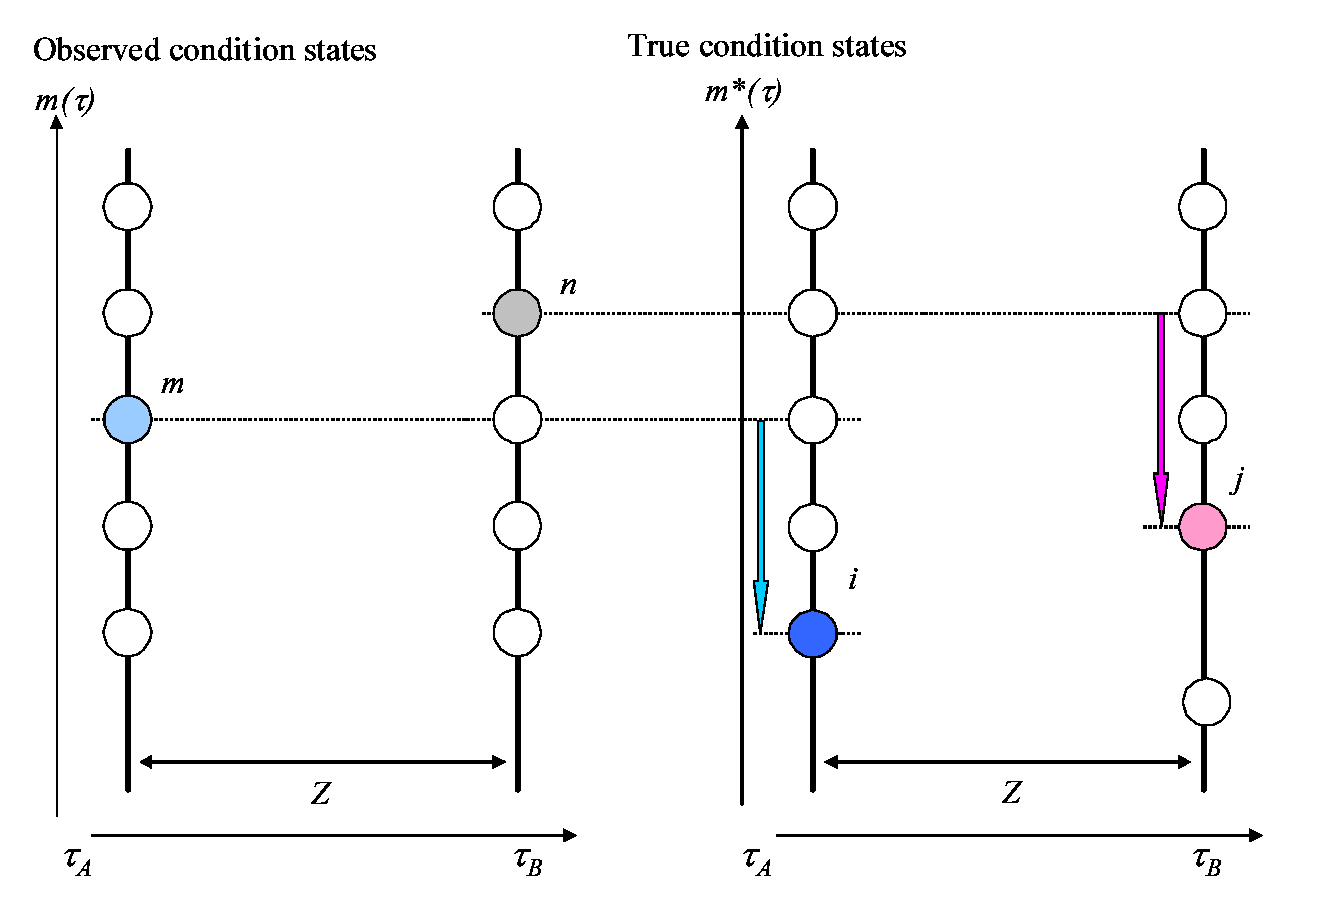
\includegraphics[scale=0.5]{fig42.eps}\\
Note) Observed values of states for $\tau_A, \tau_B$ are higher than the true condition state values due to measurement errors.
\end{footnotesize}
\end{center}
\caption{Degree of Measurement Errors.}
\label{fig42}
\end{figure}
%%%

According to \citet{humplick}, measurement errors can be assigned as random variables. With this assumption, the discrete probability distribution of observed condition state $m$ can be described by using likelihood function $f_i(m|\mbox{\boldmath$\alpha$}_i)$. We can explain from the function that the probability of the observed condition state $m$ conditionally depends on the true condition state $i$. In other words, it conditionally depends on the characteristic parameter $\mbox{\boldmath$\alpha$}_i$ of the probability distribution of the true condition state $i$.

We further assume $z$ as the duration between two consecutive inspection times $\tau_A$ and $\tau_B$. On the same road section, at inspection time $\tau_B$, the observed condition states and true condition states are supposed to be $m(\tau_B)=n$ and $m^\ast(\tau_B)=j$ respectively. Since the process of deterioration progresses in an  uncertain manner, there is no concrete guarantee of having any correlation between the two  condition states $n$ and $j$. 

As for the transition pattern between the condition states in the period $[\tau_A,\tau_B)$, it is $m\rightarrow n$ for the observed condition states and $i\rightarrow j$ for the true condition states. In term of Markov transition probability, however, we are able to estimate only the Markov transition probability $\pi_{mn}$, while  the Markov transition probability $\pi_{ij}$ is hidden. Because of the hidden characteristics, the hidden Markov model is then proposed, with its focus on estimating  the true Markov transition probability $\pi_{ij}$. Further to the meaning of the likelihood function $f_i(m|\mbox{\boldmath$\alpha$}_i)$, it can be described as a mixing part of the conventional Markov transition probability (refer to Chapter \ref{Chapter2}). Thus, one of important roles of the hidden Markov model is to estimate the condition probability distribution $f_i(m|\mbox{\boldmath$\alpha$}_i)$.
%%%%
\section{Exponential Markov Deterioration Hazard Model}
\label{43}
Reference is mainly made to section \ref{233}, in which, the exponential Markov Hazard model has been extensively explained. For convenience of reading in subsequent parts of this Chapter, following equation is given as  the obtained results from section \ref{233} in Chapter \ref{Chapter2}:
%
\begin{eqnarray}
&& \pi_{ij}(z)=\mbox{Prob}[m^\ast(\tau_B)=j|m^\ast(\tau_A)=i]  =\prod_{m=i,\neq k}^{k-1}\frac{\theta_m}{\theta_{m}-\theta_{k}} \exp (-\theta_{k}z). \label{4poi}
\end{eqnarray}
\section{Hidden Markov hazard model} \label{44}
\subsection{Mixture distribution mechanism} \label{441}
%
This section explains the mathematical formulation of the hidden Markov chain model based on mixture distribution mechanism. Assumption is referred to section \ref{422}. In fact, it is uncertain to use the probability distribution function $f_i(m|\mbox{\boldmath$\alpha$}_{i})~(i=1,\cdots,I)$ to estimate the true condition state $i$. However,  we are able to express the probabilistic dependence of the observed condition state $m(\tau_A)=m$ on the true condition state $i$ by means of the likelihood function $f_i(m|\mbox{\boldmath$\alpha$}_{i})~(i=1,\cdots,I)$:

\begin{eqnarray}
&& \ell(m(\tau_A)=m)=\sum_{i=1}^I \pi_i(\tau_A)
f_i(m|\mbox{\boldmath$\alpha$}_{i}).\label{mixture1}
\end{eqnarray}
where $\pi_i(\tau_A)$ is the probability of the true condition state $i$ at inspection time $\tau_A$. Equation (\ref{mixture1}) depicts the conditional probability distribution of the observed condition state $m(\tau_A)=m$ on the true condition state $i$. In other words, it portrays the conditional probability distribution of the observed condition state $m(\tau_A)=m$ by averaging the distributed values of measurement errors over the range of the true condition states. A model with mixing mechanism of measurement errors is referred as a mixture distribution model \cite{die}.

Similarly, the probability distribution of the observed condition states at inspection time $\tau_B=\tau_A+z$ $(\tau_A<\tau_B)$ can be described by means of mixing form. The likelihood function $\ell(m(\tau_A)=m,m(\tau_B)=n)$, to which the observed condition state $m(\tau_B)=n$ at inspection time $\tau_B$ can be defined as
\begin{eqnarray}
&& \ell_i(m(\tau_B)=n)=\sum_{j=i}^I \pi_{ij}(z) f_j(n|\mbox{\boldmath$\alpha$}_j).
\end{eqnarray}
As a matter of course, the likelihood distribution function of the observed condition state $\ell(m(\tau_B)=n)$ at inspection time $\tau_B$ conditionally depends on the probability $\pi_i(\tau_A)$ despise the fact that the true condition state $i$ at inspection time $\tau_A$ is absolutely hidden. Following equation details the conditional dependency in the likelihood function:
\begin{eqnarray}
&& \hspace{-10mm}\ell(m(\tau_B)=n) =\sum_{i=i}^I \pi_i(\tau_A) \ell_i(m(\tau_B)=n) = \sum_{i=i}^I \pi_i(\tau_A) \sum_{j=i}^I \pi_{ij}(z) f_j(n|\mbox{\boldmath$\alpha$}_j). \label{ku}
\end{eqnarray}
As a result, the likelihood function $\ell(m(\tau_A)=m,m(\tau_B)=n)$, at which we observe the condition state $m(\tau_A)=m$ at inspection time $\tau_A$ and the condition state $m(\tau_B)=n$ at inspection time $\tau_B$, can be defined:
\begin{eqnarray}
&& \hspace{-10mm} \ell(m(\tau_A)=m,m(\tau_B)=n) = \sum_{i=1}^I \pi_i(\tau_A) f_i(m|\mbox{\boldmath$\alpha$}_{i})\left(\sum_{j=i}^I \pi_{ij}(z)  f_j(n|\mbox{\boldmath$\alpha$}_j)\right). \label{ksu}
\end{eqnarray}
It is noticed from equation (\ref{ksu}) that the probability distribution functions $f_i(m|\mbox{\boldmath$\alpha$}_{i})$ and $f_j(n|\mbox{\boldmath$\alpha$}_{j})$ are in strong correlation with each others through the Markovian transition probability $\pi_{ij}(z)$. In other words, the distribution of the observed condition state depends on the hidden characteristics or measurement errors at respective inspection time $\tau_A$ and $\tau_B$.
%%%%%%%%%%%%
\subsection{Initial values of the condition states} \label{442}
As can be seen from equation (\ref{ksu}), there are three unknown components, the initial distribution $\pi_i(\tau_A)$, the probability distribution function $f_i(m|\mbox{\boldmath$\alpha$}_{i})$ and the Markov transition probability $\pi_{ij}(z)$. The value of the initial probability distribution $\pi_i(\tau_A)$ is regarded as a transcendental information. The initial probability distribution can be assumed as a variable of non-parametric distribution. However, assuming it as a non-parametric variable limits the study for a large number of monitoring data since characteristic variables  concerning a road section do not share the same values with the other road sections. It is therefore advisable to determine the initial value of condition state immediately after any $M\&R$ action. Because, by implementing $M\&R$ actions, the condition state of a road section will become good again, with $i=1$. For example, if a $M\&R$ action is carried out just before time $\tau_0$, the initial probability distribution can be defined as
\begin{eqnarray}
&& \mbox{\boldmath$\pi$}(\tau_0)=\{\pi_1(\tau_0),\cdots,\pi_I(\tau_0)\} =(1,0,\cdots,0).
\end{eqnarray}
Evidently, the properties of the vector $\mbox{\boldmath$\pi$}(\tau_0)$ is measurable. Thus, if $M\&R$ actions are implemented at alternative times $\tau_1,\cdots,\tau_T$, the initial value of probability distribution $\pi_i(\tau_A)$ can also be defined. To come up with a general likelihood function for the conditional probability distribution of the observed condition states $m$, the observed condition states after $M\&R$ actions at times $\tau_t$ $(t=1,...,T)$ are assumed as $m(\tau_t)=m_t$. The durations between two consective $M\&R$ actions from $t-1$ to $t$ are denoted as $z_{t}~(t=1,\cdots,T)$. As a result, likelihood function ${\cal L}(\mbox{\boldmath$\alpha$},\mbox{\boldmath$m$},\mbox{\boldmath$z$})$, which describes the conditional probability distribution of the observed condition states $\mbox{\boldmath$m$}=(m_1,\cdots,m_T)$, can be recurrently defined:
\begin{eqnarray}
&& {\cal L}(\mbox{\boldmath$\alpha$},\mbox{\boldmath$m$},\mbox{\boldmath$z$})=\sum_{j=1}^I \pi_{1j}(z_1)f_j(m_1|\mbox{\boldmath$\alpha$}_j)\ell_j(1), \label{mu0} \\
&& \ell_h(t)=\sum_{j=h}^I \pi_{hj}(z_t)f_j(m_t|\mbox{\boldmath$\alpha$}_j)\ell_j(t+1) \hspace{10mm}(1 \leq t \leq T-1), \\
&& \ell_h(T)=\sum_{j=h}^I \pi_{hj}(z_T)f_j(m_T|\mbox{\boldmath$\alpha$}_j). \label{myuudo1}
\end{eqnarray}
The maximum likelihood estimation method can be used to estimate the parameters of the model by applying numerial analysis with the objective likelihood function. However, the method exerts to have its limitation as it requires a high order of derivative and high degree of computation for solving the optimal condition of nonlinear polynomial equations.  Therefore, in view of problems in the hidden Markov model, the maximum likelihood method is not deemed as an ultimate solution \cite{titter}. Attempts to overcome the limitation of the maximum likelihood method by using Bayesian estimation have been proposed.  
%%%%%%%%%%%%%%%%%%
\subsection{Complete likelihood function} \label{443}
The distribution of measurement errors is assumed by means of a hidden variable $\mbox{\boldmath$s$}=(s_0,\cdots,s_T)$. If there is no $M\&R$ action in the inspection period, the  following condition is satisfied:
\begin{eqnarray}
&& s_0=1\leq s_1 \leq \cdots \leq s_T \leq I. \label{stk}
\end{eqnarray}
Furthermore, if the hidden variable is measureable, its value can be used to update the probability distribution of the true condition state $i$, which is hidden because of measurement errors. In addition, to identify the possibility of actual measurement of the hidden variable, a dummy variable $\delta$ is assigned with the conditions as follows:
\begin{eqnarray}
&& \delta_{ti}=\left\{
\begin{array}{ll}
1 & s_t=i\\
0 & s_t\ne i
\end{array},
\right. (t=1,\cdots,T;i=1,\cdots,I) .
\end{eqnarray}
With this assumption and according to \citet{demp}, the likelihood functions (\ref{mu0})-(\ref{myuudo1}) are then  described as follows:
\begin{eqnarray}
&& \hspace{-10mm}\tilde{\cal L}(\mbox{\boldmath$s$},\mbox{\boldmath$\alpha$},\mbox{\boldmath$m$},\mbox{\boldmath$z$}) =\prod_{i=1}^I \Big\{\pi_{1i}(z_1)^{\delta_{1i}} f_{i}(m_1|\mbox{\boldmath$\alpha$}_{i})^{\delta_{1i}}  \prod_{t=2}^T \prod_{j=i}^I \pi_{ij}(z_t)^{\delta_{t-1i}\delta_{tj}} f_{j}(m_t|\mbox{\boldmath$\alpha$}_{j})^{\delta_{tj}}\Big\} \nonumber \\
&& \hspace{10mm}=\prod_{t=1}^T \Big\{\pi_{s_{t-1}s_t}(z_t) f_{s_t}(m_t|\mbox{\boldmath$\alpha$}_{s_t})\Big\} = \prod_{t=1}^T \pi_{s_{t-1}s_t}(z_t) \prod_{t=1}^T f_{s_t}(m_t|\mbox{\boldmath$\alpha$}_{s_t}). \label{hyuudo2}
\end{eqnarray}
Equation (\ref{hyuudo2}) is referred as a complete likelihood equation \citep{dani-hed}, with a better explicit form than that in the likelihood equations (\ref{mu0})-(\ref{myuudo1}). Nevertheless, a difficulty remains at this point is how to assign a realistic value for the hidden variable $\mbox{\boldmath$s$}$ since it is unobservable. In view of probability distribution, the hidden variable $\mbox{\boldmath$s$}$ can be derived by applying the full conditional posterior distribution in Bayesian inference. In which, the prior probability distribution in Bayesian estimation is assumed as follows: 
%%%%%%%%
\begin{eqnarray}
&& \hspace{-15mm} \mbox{Prob}\{s_t=i|\mbox{\boldmath$s$}_{-t},\mbox{\boldmath$\alpha$},\mbox{\boldmath$\xi$}\} =\frac{\tilde{\cal L}(\mbox{\boldmath$s$}_{-t}^i,\mbox{\boldmath$\alpha$},\mbox{\boldmath$m$},\mbox{\boldmath$z$})}{\sum_{i=s_{t-1}}^{s_{t+1}} \tilde{\cal L}(\mbox{\boldmath$s$}_{-t}^i,\mbox{\boldmath$\alpha$},\mbox{\boldmath$m$},\mbox{\boldmath$z$})} =\frac{\omega_{it} f_i(m_t|\mbox{\boldmath$\alpha$}_i)}{\sum_{j=s_{t-1}}^{s_{t+1}} \omega_{jt} f_j(m_t|\mbox{\boldmath$\alpha$}_j)}, \label{hhu}
\end{eqnarray}
where $\mbox{\boldmath$s$}_{-t}=(s_1,\cdots,s_{t-1},s_{t+1},\cdots,s_{T}),\mbox{\boldmath$s$}_{-t}^i=(s_1,$$\cdots,$$s_{t-1},i,s_{t+1},\cdots,s_{T})$, and $s_t=i ~(i$ $\in \{s_{t-1},$$\cdots, s_{t+1}\})$. In addition, $\omega_{jt}$ satisfies 
\begin{eqnarray}
&& \omega_{jt}=\left\{
\begin{array}{ll}
\pi_{1j}\pi_{js_2} & t=1 \\
\pi_{s_{t-1}j}\pi_{js_{t+1}} & 2\leq t \leq T \\
\pi_{s_{T-1}j} & t=T
\end{array}.
\right.
\end{eqnarray}
It is clear at this point that if the posterior probability distribution of the hidden variable $s_t \in \{s_{t-1},\cdots,s_{t+1}\}$ at time $t$ is measurable, the transition probability $\pi_{ij}(z)~(i=1,\cdots,I;j=i,\cdots,I)$ and the probability distribution function $f_i(m|\mbox{\boldmath$\alpha$}_i)~(i=1,\cdots,I)$ can be ultimately estimated. It is also noted that the posterior probability distribution of the hidden variable $s_t \in \{s_{t-1},\cdots,s_{t+1}\}$ is conditionally depended on the observed value of $\mbox{\boldmath$s$}_{-t}$. 

To solve the likelihood equation (\ref{hyuudo2}), it is required to estimate the value of  hidden variable $\mbox{\boldmath$s$}$. As a result, the main task is to estimate the unknown parameters $\mbox{\boldmath$\alpha$}$ and $\mbox{\boldmath$\beta$}$, which are embedded in the transition probability functions. In fact, there is no possibility to seek for the posterior distribution of all hidden variables. Thus, MCMC simulation is recommended to use in randomly generating the hidden variable $\mbox{\boldmath$s$}$.
%%%%%%
\subsection{Conditional distribution of measurement errors} \label{444}
As earlier mentioned in section \ref{42}, the representative condition state of a road section generally happens to be the worst condition state among several condition states observed on the same section. Thus, it is possible to assume the range of observed condition state $m$ in a domain $m(m=1,...,i)$. The relationship between the observed condition state $m$ and the true condition state $i$ implies measurement errors on the same road section. Suffice it to say that the selection of the observed condition state can be considered as a random selection process. However, probabilistic inference on the value of probability distribution function $f_i(m|\mbox{\boldmath$\alpha$}_i)~(m=1,\cdots,i)$ faces some degrees of difficulty. In this research, the distribution probability function $f_i(m|\mbox{\boldmath$\alpha$}_i)~(m=1,\cdots,i)$ is assigned to satisfy the following conditions:
%%%%
\begin{eqnarray}
&& f_i(m|\mbox{\boldmath$\alpha$}_i)=\left\{
\begin{array}{ll}
0 &  \hspace{10mm} when \hspace{10mm}m > i \\
\alpha_{m}^i & \hspace{10mm} when \hspace{10mm}m \leq i
\end{array},
\right. \label{pmi}
\end{eqnarray}
where parameter $\alpha_{m}^i$ is assumed as a non-parametric constant satisfying
\begin{eqnarray}
0\leq \alpha_{m}^i \leq 1, \label{a14} \\
\sum_{m=1}^i \alpha_{m}^i=1. \label{a24}
\end{eqnarray}
The probability distribution of parameter $\alpha_m^i$ can be estimated if having enough numbers of monitoring data. This is a non-parametric approach in case of receiving no prior information regarding measurement errors. This approach has been applied in the research on the probabilistic measurement of system errors \cite{bauer,jj}. 
%%%%
\section{Estimation methodology} \label{45}
\subsection{Markov Chain Monte Carlo method} \label{451}
In statistic with Bayesian inference, the prior and posterior probability are employed with aim to estimate the values of model's parameters \cite{wago}. However, in hazard analysis, it is hard to define the prior probability distribution, even in a simple condition states hazard model \cite{ibra1}. Methods to overcome the problems in the assumption of the prior probability distribution often require numerical analyses with multi-dimensional integration, and thus remain as a limitation in Bayesian estimation.

In recent years, an appealing solution to the problem in Bayesian estimation has been proposed, with the application of MCMC simulation. The MCMC simulation technique does not require a high level of derivative and multi-dimensional integration of model's objective functions \cite{wago}. As a result, estimation results in a great deal of applied statistic research have been improved through a combination of the Bayesian estimation and MCMC simulation.

In MCMC simulation, Gibbs sampling and Metropolis Hastings (Metropolis-Hastings or MH) techniques have been extensively discussed \cite{wago}. Reference to the research on image restoration is a good example of MCMC simulation \cite{gibbs1}. Of that study, the algorithm of Gibbs sampling was used to estimate the posterior distribution in Bayesian estimation \cite{gibbs2}. In MH law, the iterative parameter $\mbox{\boldmath$\beta$}$ is defined by repeatedly generating random numbers through the conditional probability density function. In this research, we propose an extended estimation methodology to estimate the parameters of the hidden Markov model based on the literature of the Bayesian estimation for the Weibull hazard model of \citet{bayse}.

Further to the estimation parameters in hidden Markov models, analytical approach using the method of maximum likelihood has already exhibited its limitation \cite{titter,robert}. Since hidden Markov model is considered as one type of mixture distribution model, a great deal of research suggested to define a set of complete likelihood functions instead of using conventional likelihood functions \cite{die,robe}. In view of MCMC simulation, it is necessary to develop an explicit algorithm for estimating the Markov transition probability with multi-condition states. In this research, we propose an analytical approach using Bayesian estimation and MCMC simulation for estimating the Markov transition probability of the conventional exponential hazard model, which is briefly presented in Chapter \ref{Chapter2}.
%%%%%%%%%%%%%%%%%%%%%%%%
\subsection{Formulation of the model} \label{452}
Visual inspection is carried out on each section $k$ of the entire road system (with $K$ is the total number of road sections). The observed data on each section over a time-series can be denoted as $\tau_t^k~(t=1,\cdots,T^k)$, with $T^k$ as the number of inspection times for the road section $k$. Each observed condition state from the visual inspection is represented as $\bar{m}(\tau_t^k)$, with the sign $\bar{\hspace{2mm}}$ indicating the measurable data. $\bar{\mbox{\boldmath$\xi$}}=(\bar{\mbox{\boldmath$\xi$}}^1,\cdots,\bar{\mbox{\boldmath$\xi$}}^K)$ is denoted as the vector of measureable data concerning $\sum_{k=1}^K T^k$ numbers of records. 

The deterioration process of a road section is influenced by the changes in the values of characteristic variables such as traffic volume, thickness of overlay, weather, etc. The values of  characteristic variables are recorded and stored in monitoring data. To consider the effects of characteristic variables on the deterioration, vector $\bar{\mbox{\boldmath$x$}}_t^k$ is assumed to represent for characteristic variables. In addition, the duration between two consecutive visual inspections is defined as $\bar{z}_t^k=\tau_t^k-\tau_{t-1}^k$. In summary, the observed information concerning each section of a road can be symbolized as $\bar{\mbox{\boldmath$\xi$}}_t^k=(\bar{m}_t^k,\bar{z}_t^k,\bar{\mbox{\boldmath$x$}}_t^k)$, with $m(\tau_t^k)=\bar{m}_t^k$. As a result, the simultaneous probability distribution for the entire $K$ samples can be defined:
%%%%%%%%
\begin{eqnarray}
&& \hspace{3mm}\tilde{\cal L}(\mbox{\boldmath$\alpha$},\mbox{\mbox{\boldmath$s$},\boldmath$\beta$},\bar{\mbox{\boldmath$\xi$}}) 
=\prod_{k=1}^K\Bigl\{\prod_{t=1}^{T^k}\pi_{s_{t-1}^ks_t^k}(\bar{z}_t^k)\prod_{t=1}^{T^k} f_{s_t^k}(\bar{m}_t^k|\mbox{\boldmath$\alpha$}_{s_t^k})\Bigl\}\nonumber \\
&& =\prod_{k=1}^K \Bigl[\prod_{t=1}^{T^k}\alpha_{\bar{m}_t^k}^{s_{t}^k}\sum_{l=s_{t-1}^k}^{s_t^k}\Bigl\{ \prod_{i=s_{t-1}^k,\neq l}^{l-1}\frac{\theta_{i}^k}{\theta_{i}^k-\theta_{l}^k}\exp(-\theta_{l}^k\bar{z}_t^k)\Bigl\}\Bigl],
\label{hyuudo3}
\end{eqnarray}
In likelihood equation (\ref{hyuudo3}), the hazard function is described by using exponential form as
$\theta_i^k=\exp(\mbox{\boldmath$x$}^k\mbox{\boldmath$\beta$}_i^\prime)$. In order to estimate the unknown parameters and the hidden variables (measurement errors), the method using to solve the likelihood functions (\ref{mu0})-(\ref{myuudo1}) should be considered. By solving equation (\ref{hyuudo3}), the values of $\mbox{\boldmath$\alpha$}=(\mbox{\boldmath$\alpha$}_1,\cdots,\mbox{\boldmath$\alpha$}_{I-1})$, $\mbox{\boldmath$\beta$}=(\mbox{\boldmath$\beta$}_1,\cdots,\mbox{\boldmath$\beta$}_{I-1})$ and hidden variable $\mbox{\boldmath$s$}=(\mbox{\boldmath$s$}^1,\cdots,\mbox{\boldmath$s$}^K)$ can be obtained. If parameter vectors $\mbox{\boldmath$\alpha$}$ and  $\mbox{\boldmath$\beta$}$ are known, the posterior distribution of the hidden variable $s_t^k~(t=1,\cdots,T^k;k=1,\cdots,K)$ can be estimated as well. Given the condition $\mbox{\boldmath$s$}_{-t}^k=(s_1^k,\cdots,s_{t-1}^k,s_{t+1}^k,\cdots,s_{T^k}^k)$, the conditional probability, to which the hidden variable $s_t^k ~(s_t^k \in \{s_{t-1}^k,\cdots, s_{t+1}^k\})$ equals to the true condition state $i$ , is finally estimated:
%%%%%%%%%%%%
\begin{eqnarray}
&& \mbox{Prob}\{s_t^k=i|\mbox{\boldmath$s$}_{-t}^k,\mbox{\boldmath$\alpha$},\mbox{\boldmath$\xi$}\} =\frac{\omega_{it}^k f_i(m_t^k|\mbox{\boldmath$\alpha$}_i)}{\sum_{j=s_{t-1}^k}^{s_{t+1}^k} \omega_{jt}^k f_j(m_t^k|\mbox{\boldmath$\alpha$}_j)},\label{k3}
\end{eqnarray}
where
\begin{eqnarray}
&& \omega_{jt}^k=\left\{
\begin{array}{ll}
\pi_{1j}\pi_{js_2} & t=1 \\
\pi_{s_{t-1}^kj}\pi_{js_{t+1}^k} & 2\leq t \leq T^k \\
\pi_{s_{T^k-1}^kj} & t=T^k
\end{array}.
\right.
\end{eqnarray}
%%%%%%%%%%%%%%%%%%
\subsection{Bayesian estimation} \label{453}
As a common practice in Bayesian estimation, the assumption for the prior probability distribution of parameters $\mbox{\boldmath$\alpha$}$ and $\mbox{\boldmath$\beta$}$ is based on various sources of prior experience information. Any new information concerning monitoring data $\mbox{\boldmath$\xi$}$ shall be directly used for estimation of the likelihood function ${\cal L}(\mbox{\boldmath$\alpha$}$, $\mbox{\boldmath$\beta$}$, $\bar{\mbox{\boldmath$\xi$}})$. The updating rule in Bayesian estimation constantly improves the level of accuracy for prior probability distribution of the parameters. By using the most up-to-date monitoring data, the parameters $\mbox{\boldmath$ \alpha$}$ and $\mbox{\boldmath$ \beta$}$ specifying the probability density function $\rho(\mbox{\boldmath$\alpha$},\mbox{\boldmath$\beta$}|\mbox{\boldmath$\xi$})$ can be simultaneously obtained. However, according to \citet{ibra1}, just only a single time of assuming the prior probability density function cannot guarantee the accuracy of estimation results since the prior probability density function can be assumed in various ways. Thus, it is advisable to define the prior probability density function along with the continuity of visual inspections. As a rule of thumb, the influence of the prior probability density function will gradually decreases as the number of monitoring data increases.

As earlier mentioned in section \ref{444}, the constant parameter $\mbox{\boldmath$\alpha$}_i=(\alpha_1^i,\cdots,\alpha_i^i)$ in equation (\ref{pmi}) is assumed to satisfying the conditions in equations (\ref{a14}) and (\ref{a24}). On that account, we introduce the  conjugate Dirichlet distribution for the prior probability density function of the constant $\mbox{\boldmath$\alpha$}_i$:
\begin{eqnarray}
&& \eta_i(\mbox{\boldmath$\alpha$}_i|\mbox{\boldmath$\nu$}^i)=\Psi_i(\mbox{\boldmath$\nu$}^i) \prod_{m=1}^i (\alpha_m^i)^{\nu_m^i-1}, \label{nu11} \\&& \Psi_i(\mbox{\boldmath$\nu$}^i)=\frac{\Gamma(\nu_1^i+\cdots+\nu_i^i)}{\Gamma(\nu_1^i)\cdots\Gamma(\nu_i^i)} \hspace{3mm} and \hspace{3mm} \sum_{m=1}^i \alpha_m^i =1. \nonumber
\end{eqnarray}
It is noted that the Direclet distribution infers a constant parameter $\mbox{\boldmath$\nu$}^i=(\nu_1^i,\cdots,\nu_i^i)$, which is spontaneously satisfying the constant parameter $\mbox{\boldmath$\alpha$}_i$ in equations (\ref{a14}) and (\ref{a24}).

Assumption for the prior probability density function of parameter $\mbox{\boldmath$\beta$}_i$ can be  defined in the next step. The conjugate multidimensional normal distribution $\mbox{\boldmath$\beta$}_i \sim {\cal N}_M(\mbox{\boldmath$\zeta$}_i,\mbox{\boldmath$\Sigma$}_i)$ is assumed for the prior probability density function in $M$ dimension:
 %
   \begin{eqnarray}
      && \hspace{-8mm}
      h(\mbox{\boldmath$\beta$}_i|
      \mbox{\boldmath$\zeta$}_i,\mbox{\boldmath$\Sigma$}_i)
      = \frac{1}{(2\pi)^{\frac{M}{2}}\sqrt{|\mbox{\boldmath$\Sigma$}_i|}}
      \cdot \exp\Big\{-\frac{1}{2}(\mbox{\boldmath$\beta$}_i
      -\mbox{\boldmath$\zeta$}_i)
      \mbox{\boldmath$\Sigma_i$}^{-1}
      (\mbox{\boldmath$\beta$}_i-\mbox{\boldmath$\zeta$}_i)^\prime\Big\},
            \label{Kseiki}
   \end{eqnarray}
 %
 %
where $\mbox{\boldmath$\Sigma$}_i$ of ${\cal N}_M(\mbox{\boldmath$\zeta$}_i,\mbox{\boldmath$\Sigma$}_i)$  and $\mbox{\boldmath$\zeta$}_i$ are the covariance matrix and the standard covariance of the prior distribution respectively. As a result, a proportional result of the probability density function $\rho(\mbox{\boldmath$\alpha$},\mbox{\boldmath$\beta$}|\mbox{\boldmath$s$},\mbox{\boldmath$\xi$})$ can be re-formulated:
 %
   \begin{eqnarray}
      && \rho(\mbox{\boldmath$\alpha$},\mbox{\boldmath$\beta$}|\mbox{\boldmath$s$},\mbox{\boldmath$\xi$})   \propto \tilde{\cal L}(\mbox{\boldmath$\alpha$},\mbox{\boldmath$\beta$},\mbox{\boldmath$s$},\mbox{\boldmath$\xi$})\prod_{i=1}^{I-1}\Bigl\{h(\mbox{\boldmath$\beta$}_i|\mbox{\boldmath$\mu$}_i,\mbox{\boldmath$\Sigma$}_i) \eta_i(\mbox{\boldmath$\alpha$}_i|\mbox{\boldmath$\nu$}^i)\Bigr\}
      \nonumber \\
      && \hspace{10mm}\propto \prod_{k=1}^K \left[ \prod_{t=1}^{T^k} \sum_{l=s_{t-1}^k}^{s_t^k} \Bigl\{ \prod_{i=s_{t-1}^k,\neq l}^{l-1}\frac{\theta_i^k}{\theta_{i}^k-\theta_{l}^k} \exp (-\theta_{l}^kz_t^k)\Bigr\} \right.
      \cdot \nonumber \\
  &&   \hspace{20mm} \prod_{i=1}^{I-1}\exp\Big\{-\frac{1}{2}
      (\mbox{\boldmath$\beta$}_i-\mbox{\boldmath$\zeta$}_i)
      \mbox{\boldmath$\Sigma_i$}^{-1}
      (\mbox{\boldmath$\beta$}_{i}-\mbox{\boldmath$\zeta$}_i)^\prime\Big\} \nonumber \\
      && \hspace{20mm}\left.\hspace{2mm}\cdot \left(\prod_{t=1}^{T^k} \alpha_{\bar{m}_t^k}^{s_{t}^k}\right)\left( \prod_{i=1}^{I}\prod_{m=1}^{i} (\alpha_m^i)^{\nu_m^{i}-1}\right) \right]. \label{post1}
   \end{eqnarray}
 %
 \subsection{Gibbs sampling} \label{454}
As the matter of fact, a direct estimation for the probability density function $\rho(\mbox{\boldmath$\alpha$},\mbox{\boldmath$\beta$}|\mbox{\boldmath$\xi$})$ in hidden Markov deterioration hazard model is impracticable. By using the MCMC simulation, specimens of the parameters $\mbox{\boldmath$\alpha$}$ and $\mbox{\boldmath$\beta$}$ can be alternately extracted from the probability density function \cite{gibbs1}. In equation (\ref{post1}), the parameters $\mbox{\boldmath$\alpha$}$ and $\mbox{\boldmath$\beta$}$ can be mutually used to express the probability density function. Approximation of $\rho(\mbox{\boldmath$\alpha$}|\mbox{\boldmath$s$}, \mbox{\boldmath$\xi$})$ and $ \rho(\mbox{\boldmath$\beta$}|\mbox{\boldmath$s$},\mbox{\boldmath$\xi$})$ can be further described as follows:
%%%%%%%%%%
\begin{eqnarray}
&& \hspace{-3mm} \rho(\mbox{\boldmath$\alpha$}|\mbox{\boldmath$s$},\mbox{\boldmath$\xi$}) \propto \Bigl( \prod_{k=1}^K \prod_{t=1}^{T^k} \alpha_{\bar{m}_t^k}^{s_{t}^k} \Bigr)
\Bigl\{ \prod_{i=1}^I \prod_{m=1}^{i} (\alpha_m^{i})^{\nu_m^{i}-1}\Bigr\},
\label{k1}
\\
&& \hspace{-3mm} \rho(\mbox{\boldmath$\beta$}|\mbox{\boldmath$s$},\mbox{\boldmath$\xi$}) \propto \Big\{ \prod_{k=1}^K \Bigl[\prod_{t=1}^{T^k} \sum_{l=s_{t-1}^k}^{s_t^k} 
\Bigl[ \prod_{i=s_{t-1}^k,\neq l}^{l-1}\frac{\theta_i^k}{\theta_{i}^k-\theta_{l}^k} \exp (-\theta_{l}^kz_t^k)\Bigr]\Bigr\}. \nonumber \\
&& \hspace{20mm}\prod_{i=1}^{I-1}\exp\Big\{-\frac{1}{2}
      (\mbox{\boldmath$\beta$}_i-\mbox{\boldmath$\zeta$}_i)
      \mbox{\boldmath$\Sigma_i$}^{-1}
      (\mbox{\boldmath$\beta$}_{i}-\mbox{\boldmath$\zeta$}_i)^\prime\Big\}.  \label{k2}
\end{eqnarray}
The conditional posterior distribution of the hidden variable $\mbox{\boldmath$s$}$ can be expressed in equation (\ref{k3}). A detailed procedure of the analytical approach using the Bayesian estimation and the MCMC simulation is drawn in Figure. \ref{fig44}. To explain the flow of algorithm in the figure, a detail of procedure is given in the subsequent writing of this section.
\begin{figure}
\begin{footnotesize} 
\begin{center}
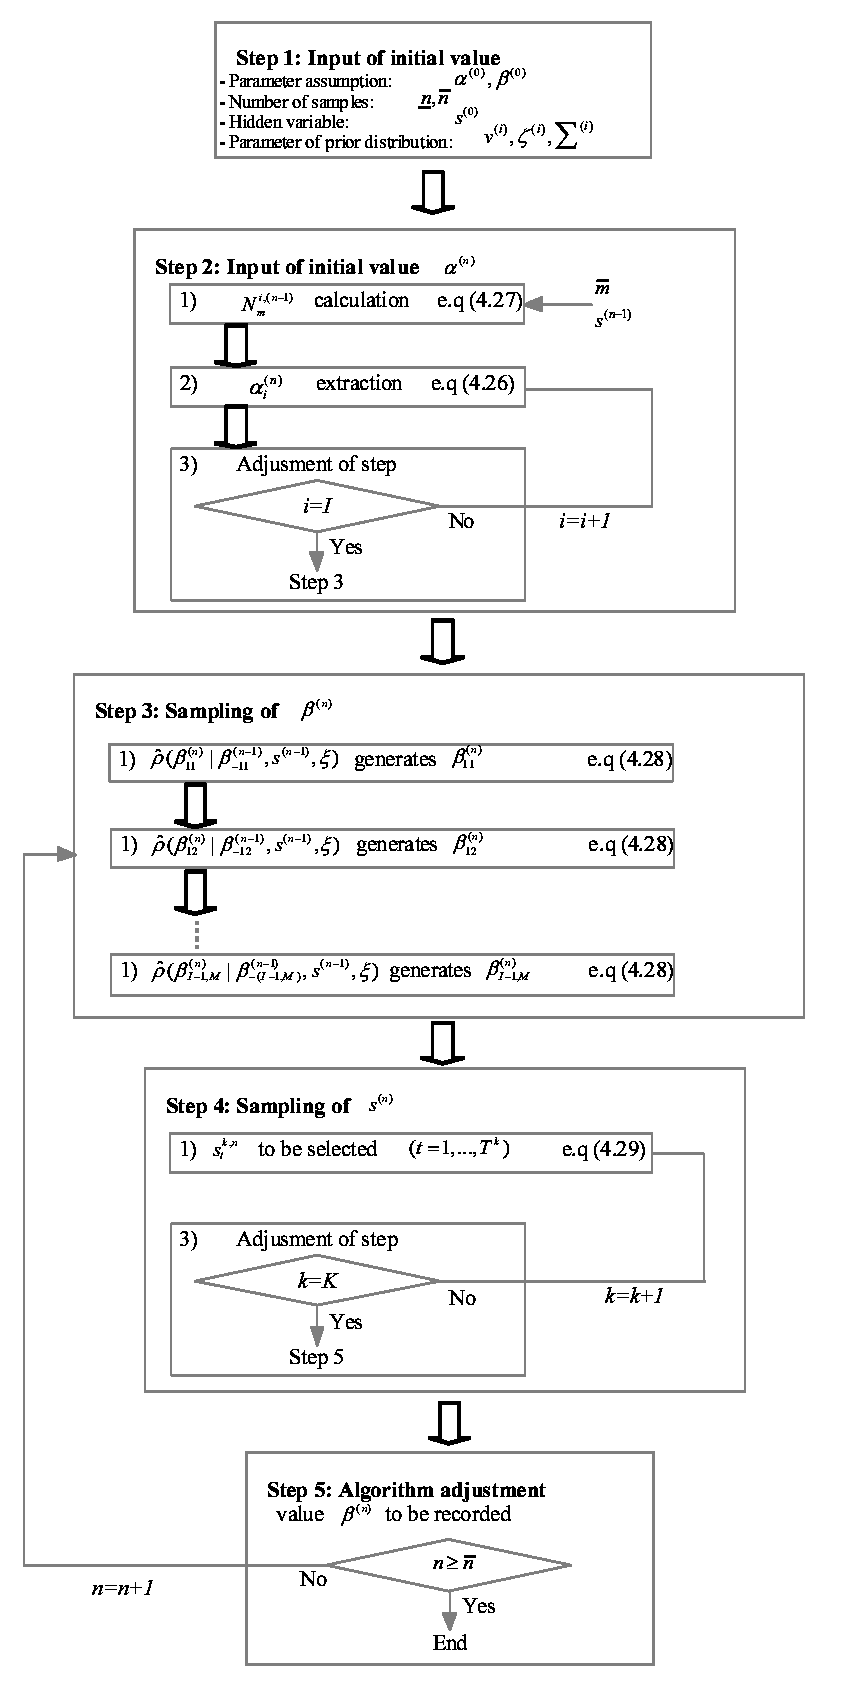
\includegraphics[scale=0.8]{fig44.eps}
\end{center}
\caption{Flowchart of Bayesian Estimation for Hidden Markov Model}
\label{fig44}
\end{footnotesize}
\end{figure}
%%%%%%%%%%%%
\subsubsection{Step 1: Initial parameter values} \label{4541}
Parameter vectors $\mbox{\boldmath$\nu$}^i~(i=1,\cdots,I)$, $\mbox{\boldmath$\zeta$}_i$, and $ \mbox{\boldmath$\Sigma$}_i~(i=1,\cdots,I-1)$ of the prior probability distribution in equations (\ref{nu11}) and (\ref{Kseiki}) have an arbitrarily set of values. The value of the hidden variable $\mbox{\boldmath$s$}^{(0)}=(\mbox{\boldmath$s$}^{(1,0)},\cdots,\mbox{\boldmath$s$}^{(K,0)})$ is initially chosen so as to satisfying $\mbox{\boldmath$s$}^{(k,0)}=(s_1^{k,0},\cdots,s_T^{k,0})$, $1\leq s_1^{k,0}\leq \cdots \leq s_T^{k,0}\leq I$, and $m_t^k\leq s_t^{k,0}~(t=1,\cdots,T;k=1,\cdots,K)$. The influence of the initial values $\mbox{\boldmath$\alpha$}^{(0)}$ and $\mbox{\boldmath$\beta$}^{(0)}$ gradually becomes weaker as more information generated by MCMC simulation is accumulated. To begin with the iteration, a sampling number $n$ in MCMC simulation is assigned as $n=1$.
%%%%%%%%%%%%%%
\subsubsection{Step 2: Sampling of the parameter $\mbox{\boldmath$\alpha$}^{(n)}$} 
\label{4542}
This section describes the estimation of $\mbox{\boldmath$\alpha$}^{(n)}=(\mbox{\boldmath$\alpha$}_1^{(n)},\cdots,\mbox{\boldmath$\alpha$}_{I-1}^{(n)})$ based on the prior hidden variable $\mbox{\boldmath$s$}^{(n-1)}$. The probability density function $\rho(\mbox{\boldmath$\alpha$}^{(n)}|\mbox{\boldmath$s$}^{(n-1)},\mbox{\boldmath$\xi$})$ in equation (\ref{k1}) can be re-written, with an extended description $\mbox{\boldmath$\alpha$}_i^{(n)}$ $=(\alpha_m^{i,n}:m=1,\cdots,i)$:
\begin{eqnarray}
&&  \tilde{\rho}(\mbox{\boldmath$\alpha$}_i^{(n)}|\mbox{\boldmath$s$}^{(n-1)},\mbox{\boldmath$\xi$}) 
 \propto \left\{ \prod_{k=1}^K \prod_{t=1}^{T^k} \alpha_{\bar{m}_t^k}^{s_{t}^{k,(n-1)}} \right\}\left\{\prod_{m=1}^{i} (\alpha_m^{i,n})^{\nu_m^{i}-1} \right\}  \nonumber \\
 && \hspace{20mm}=\prod_{m=1}^i (\alpha_m^{i,n})^{\nu_m^{i}+N_m^{i,(n-1)}-1}, \label{dir}
\end{eqnarray}
where $N_m^{i,(n-1)}$ is defined in the following equation, particularly when the values of the condition state $\bar{\mbox{\boldmath$m$}}$ and the hidden variable $\mbox{\boldmath$s$}^{(n-1)}$ are available:
\begin{eqnarray}
&& N_m^{i,(n-1)}=\#\Big\{\bar{m}_t^k=m \cap s_t^{k,(n-1)}=i\Big\}. \label{lllll}
\end{eqnarray}
The indication $\#\{\}$ in equation (\ref{lllll}) presents the number of measurable samples, to which the equation in the parentheses $\{�\}$ is referred. The parameter $\mbox{\boldmath$\alpha$}$ in equation (\ref{dir}) is assumed to follow the Dirichlet distribution, with its parameter as $\nu_m^{i}+N_m^{i,(n-1)}-1$. The parameters of the Dirichlet distribution is subsequently updated by using the extracted samples  $\mbox{\boldmath$\alpha$}_i^{(n)}=(\alpha_1^{i,(n)}, \cdots,\alpha_{i}^{i,(n)})$ through Gibbs sampling. It is noted that the samples of the parameter $\mbox{\boldmath$\alpha$}_i^{(n)}$ are evaluated from the entire range of the condition state $i(i=1,...,I)$.
%%%%%%%%%%%
\subsubsection{Step 3: Sampling of the parameter $\mbox{\boldmath$\beta$}^{(n)}$} \label{4543}
This section describes an algorithm for estimating the unknown parameter $\mbox{\boldmath$\beta$}$ of the multi-stage exponential hazard model (See the Appendix). Additional notation of the unknown parameter is $\mbox{\boldmath$\beta$}_{-eq}$. It is noticed from the notation that the element $\beta_{eq}$ $(e,q)~(e,q=1,\cdots,M)$ is excluded from the list of the unknown parameter $\mbox{\boldmath$\beta$}$. Thus, we formulated the conditional probability density function $\rho(\beta_{eq}|\mbox{\boldmath$\beta$}_{-eq},\mbox{\boldmath$s$},\mbox{\boldmath$\xi$})$ of $\beta_{eq}$ based on the assumed value of $\mbox{\boldmath$\beta$}_{-eq}$ in equation (\ref{k2}):
%
   \begin{eqnarray}
      && \hspace{-5mm} \hat{\rho}(\beta_{eq}|\mbox{\boldmath$\beta$}_{-eq},\mbox{\boldmath$s$},
      \mbox{\boldmath$\xi$}) \propto \prod_{i=1}^{e} \prod_{j=e}^I \prod_{k=1}^K  \prod_{t=1}^{T^k} \Bigl\{ \prod_{l=i}^{j-1} (\theta_l^k)^{\delta_{ij}^{tk}-\delta_{ie}^{tk}} \sum_{h=i}^{j} 
      \cdot \prod_{l=i,\neq h}^{h-1}\frac{1}{\theta_{l}^k-\theta_{h}^k} \exp (-\theta_{h}^k z_t^k)\Bigl\}^{\delta_{ij}^{tk}} \nonumber \\
      &&\hspace{50mm} \cdot \prod_{i=1}^{I-1}\exp\Big\{-\frac{1}{2}
      (\mbox{\boldmath$\beta$}_i-\mbox{\boldmath$\zeta$}_i)
      \mbox{\boldmath$\Sigma_i$}^{-1}
      (\mbox{\boldmath$\beta$}_{i}-\mbox{\boldmath$\zeta$}_i)^\prime\Big\}\Bigr] \nonumber \\
      && \hspace{2mm} \propto
\prod_{i=1}^{e} \prod_{j=e}^I \prod_{k=1}^K  \prod_{t=1}^{T^k} \Bigl[ \prod_{l=i}^{j-1} \{\exp(\beta_{eq} x_q^k)\}^{\delta_{ij}^{tk}-\delta_{ie}^{tk}}  
      \sum_{h=i}^{j} \prod_{l=i,\neq h}^{h-1}\frac{1}{\theta_{l}^k-\theta_{h}^k} \exp (-\theta_{h}^k z_t^k)\Bigl]^{\delta_{ij}^{tk}} \nonumber \\
&& \hspace{50mm} \exp\Big\{-\frac{\sigma_{e}^{qq}}{2}(\beta_{eq}-\hat{\zeta}_{e}^q)^2 \Big\}. \nonumber \\
&& \hspace{50mm}
      \hat{\zeta}_{e}^q
      = \zeta_{e}^q+\sum_{h=1,\neq q}^{M}(\beta_{eh}-\zeta_{e}^h)\sigma_e^{hq},
       \label{condition1}
      \end{eqnarray}
%
%
where $\delta_{ie}^{tk}$ and $\delta_{ij}^{tk}$ are dummy variables:
\begin{eqnarray}
&& \delta_{ie}^{tk}=\left\{
\begin{array}{ll}
1 & \hspace{2mm} \text{when} \hspace{2mm} s_{t-1}^k=i=e\\
0 &  \text{otherwise}
\end{array}
\right. 
\hspace{3mm} and \hspace{3mm} \delta_{ij}^{tk}=\left\{
\begin{array}{ll}
1 & \hspace{2mm} \text{when} \hspace{2mm} s_{t-1}^k=i,~s_t^k=j \\
0 & \text{otherwise}	
\end{array},
\right. \nonumber
\end{eqnarray}
$\zeta_{e}^q$ and $\sigma_{e}^{hq}$ are the prior expected values of the vector $\mbox{\boldmath$\zeta$}_e$ and the prior standard covariance of entire procession $\mbox{\boldmath$\Sigma_e$}^{-1}$ with respect to condition state $q$ and $(h,q)$. In addition, $\sum_{h=1,\neq q}^{M}$ is the summation of all condition states from $\sum_{h=1,\neq q}^{M}$, excluding the condition state $q$. The expected condition state is generated by using the conditional probability density functions. By using the generated condition states, we can come up with the posterior distribution of the parameter $\mbox{\boldmath$\beta$}$. A detailed MCMC simulation for estimating the posterior distribution is further presented in the subsequent writing. However, to this point, a summation of the random sampling procedure for the parameter $\mbox{\boldmath$\beta$}^{(n)}=(\beta_{11}^{(n)},\cdots,\beta_{I-1M}^{(n)})$ is presented as follows:
%%%
\begin{itemize}
\item {Step 3.1 - value of parameter $\beta_{11}^{(n)}$ is randomly generated from 
$\hat{\rho}(\beta_{11}^{(n)}|\mbox{\boldmath$\beta$}_{-11}^{(n-1)}$, $\mbox{\boldmath$s$}^{(n-1)},\mbox{\boldmath$\xi$})$}.
%%%
\item{Step 3.2 - value of parameter $\beta_{12}^{(n)}$ is randomly generated from $\hat{\rho}(\beta_{12}^{(n)}|\mbox{\boldmath$\beta$}_{-12}^{(n-1)}$, $\mbox{\boldmath$s$}^{(n-1)},\mbox{\boldmath$\xi$})$}.
%%%
\item{Step 3.3 - similar procedure in step 3.1 and step 3.2 is repeated.}
%%
\item{Step 3.4 - value of parameter $\beta_{I-1M}^{(n)}$ is randomly generated from  $\hat{\rho}(\beta_{I-1,M}^{(n)}| \\ \mbox{\boldmath$\beta$}_{-(I-1M)}^{(n-1)},  \mbox{\boldmath$s$}^{(n-1)},\mbox{\boldmath$\xi$})$.}
\end{itemize}
Gibbs sampling is applied to generate the condition states from $(I-1)M$ conditional posterior probability density functions. The so-called ``adaptive sampling rejection'' \cite{gilks} is used as a technique to generate the specimens of the parameter in the posterior distribution, which is explained in equation (\ref{condition1}).
%%%%%%%%%%%%%%
\subsubsection{Step 4: Updating the hidden variable} \label{4544}
Given the prior value of the hidden variable $\mbox{\boldmath$s$}_{-t}^{k,(n-1)}=(s_1^{k,n},\cdots,s_{t-1}^{k,n},s_{t+1}^{k,(n-1)},\cdots,s_{T^k}^{k,(n-1)})$, a new hidden variable $\mbox{\boldmath$s$}^{(n)}$ is randomly selected based on the conditional probability law in equation (\ref{k3}). Random generation applies for all condition states $s_t^{k,n} ~(s_t^{k,n} \in \{s_{t-1}^{k,n},\cdots, s_{t+1}^{k,(n-1)}\})$. Thus, we can come up with the conditional probability for the hidden variable $s_t^{k,n} ~(s_t^{k,n} \in \{s_{t-1}^{k,n},\cdots, s_{t+1}^{k,(n-1)}\})$:
%%%
\begin{eqnarray}
&& \hspace{-15mm} \mbox{Prob}\{s_t^k=i|\mbox{\boldmath$\alpha$},\mbox{\boldmath$s$}_{-t}^{k,(n-1)},\mbox{\boldmath$\xi$}\} 
 =\left\{
\begin{array}{l}
\frac{\omega_{it}^{k,(n-1)} f_i(m_t^k|\mbox{\boldmath$\alpha$}_i^{(n)})}{\sum_{j=1}^{s_{2}^{k,(n-1)}} \omega_{jt}^{k,(n-1)} f_j(m_t^k|\mbox{\boldmath$\alpha$}_j^{(n)})} \hspace{10mm} (at \hspace{5mm} t=1) \\
\frac{\omega_{it}^{k,(n-1)} f_i(m_t^k|\mbox{\boldmath$\alpha$}_i^{(n)})}{\sum_{j=s_{t-1}^{k,n}}^{s_{t+1}^{k,(n-1)}} \omega_{jt}^{k,(n-1)} f_j(m_t^k|\mbox{\boldmath$\alpha$}_j^{(n)})} \hspace{10mm} (2\leq t <T^k) \\
\frac{\omega_{it}^{k,(n-1)} f_i(m_t^k|\mbox{\boldmath$\alpha$}_i^{(n)})}{\sum_{j=s_{t-1}^{k,n}}^I \omega_{jt}^{k,(n-1)} f_j(m_t^k|\mbox{\boldmath$\alpha$}_j^{(n)})} \hspace{10mm}(at \hspace{5mm}t=T^k) 
\end{array},
\right.\label{k33}
\end{eqnarray}
where
\begin{eqnarray}
&& \omega_{jt}^{k,(n-1)}=\left\{
\begin{array}{ll}
\pi_{1j}\pi_{js_2^{k,(n-1)}} & t=1 \\
\pi_{s_{t-1}^{k,n}j}\pi_{js_{t+1}^{k,(n-1)}} & 2\leq t < T^k \\
\pi_{s_{T^k-1}^{k,n}j} & t=T^k
\end{array}.
\right.
\end{eqnarray}
The hidden variable $s_t^{k,n}~(t=1,\cdots,T^k)$ is estimated one after the other,  starting from $t=1$ for all number of the sample $k~(k=1,\cdots,K)$.
%%%%%%%%%%%%%%
\subsubsection{Step 5: Determining algorithm adjustment} \label{4545}
After step \ref{4544}, value of the parameters $\mbox{\boldmath$\alpha$}^{(n)}$, $\mbox{\boldmath$\beta$}^{(n)}$ and the hidden variable $\mbox{\boldmath$s$}^{(n)}$ are recorded. At the iteration $n=n+1$, the program returns to the step \ref{4542}. If the algorithm satisfies $n\leq \overline{n}$, the program will terminate. 

A major concern is the number of the condition state $n$ generated by the program. The number should be carefully examined. In several cases, the steady condition states could not be reached even though a large number of condition states had been accumulated. It is therefore desirable to eliminate the problem by introducing a minimum set of the parameter value as $\underline{n}$. In fact, values of the parameters $\mbox{\boldmath$\alpha$}^{(n)}$ and $\mbox{\boldmath$\beta$}^{(n)}~(n=\underline{n}+1,\underline{n}+2,\cdots,\overline{n})$ are embedded in the posterior probability density function $\rho(\mbox{\boldmath$\alpha$},\mbox{\boldmath$\beta$}|\mbox{\boldmath$\xi$})$ through the Gibbs sampling. As a result, the estimation for the posterior distribution of the parameters $\mbox{\boldmath$\alpha$},\mbox{\boldmath$\beta$}$ becomes analytical feasible. To verify the estimation results, we applied the Geweke statistical test.  
%%%% 
 \subsection{Posterior distribution statistic} \label{455}
Statistical testing for the parameter $\mbox{\boldmath$\alpha$}$ and $\mbox{\boldmath$\beta$}$ can be carried out based on the samples generated by using the MCMC simulation. However, in the simulation, the probability density function $\rho(\mbox{\boldmath$\alpha$},\mbox{\boldmath$\beta$}|\mbox{\boldmath$\xi$})$ cannot  be considered as an analytical function. Therefore, instead of using the full parametric approach for statistical testing, non-parametric approach is recommended. From the Gibbs sampling, the samples concerning $\mbox{\boldmath$\theta$}^{(n)}=(\mbox{\boldmath$\alpha$}^{(n)},\mbox{\boldmath$\beta$}^{(n)})~(n=1,\cdots,\overline{n})$ are generated. Among the generated samples, the first $\underline{n}$ samples will be removed. A new set of samples will then be defined as a replacement, with its subcriptions as ${\cal M}=\{\underline{n}+1,\cdots,\overline{n})$. By applying this approach, the joint probability distribution functions $G(\mbox{\boldmath$\alpha$})$ and $G(\mbox{\boldmath$\beta$})$ can be defined:
 %
 %
   \begin{eqnarray}
 && G(\mbox{\boldmath$\alpha$})
      =\frac{\mbox{\#}(\mbox{\boldmath$\alpha$}^{(n)}
      \leq \mbox{\boldmath$\alpha$}, n\in {\cal M})}
      {\overline{n}-\underline{n}}, \\
      && G(\mbox{\boldmath$\beta$})
      =\frac{\mbox{\#}(\mbox{\boldmath$\beta$}^{(n)}
      \leq \mbox{\boldmath$\beta$}, n\in {\cal M})}
      {\overline{n}-\underline{n}},
   \end{eqnarray}
 %
 %
where $\mbox{\#}(\mbox{\boldmath$\beta$}^{(n)} \leq \mbox{\boldmath$\beta$}, n\in {\cal M})$ is regarded as the total number of samples, from which the logical expression $\mbox{\boldmath$\beta$}^{(n)} \leq \mbox{\boldmath$\beta$}, n\in {\cal M}$ is satisfied. Moreover, the expected values of the posterior distribution of $\tilde{\mbox{\boldmath$\zeta$}_i}(\mbox{\boldmath$\beta$}_i)$ and standard covariance $\tilde{\mbox{\boldmath$\Sigma$}_i}(\mbox{\boldmath$\beta$}_i)$ are defined respectively as follows:
%
   \begin{eqnarray}
      && \hspace{-7mm}
      \tilde{\mbox{\boldmath$\zeta$}_i}(\mbox{\boldmath$\beta$}_i)=
      (\tilde{\zeta}(\beta_{i,1}),\cdots,\tilde{\zeta}
      (\beta_{i,M}))^\prime =\Big(\sum_{n=\underline{n}+1}^{\overline{n}}
      \frac{\beta_{i,1}^{(n)}}{\overline{n}-\underline{n}},
      \cdots, \sum_{n=\underline{n}+1}^{\overline{n}}
      \frac{\beta_{i,M}^{(n)}}{\overline{n}-\underline{n}}\Big)^\prime,
      \label{mu3} \\
 %
      && \hspace{-7mm}
      \tilde{\mbox{\boldmath$\Sigma$}_i}(\mbox{\boldmath$\beta$}_i)=
      \left(
      \begin{array}{lll}
         \tilde{\sigma}^2(\beta_{i,1}) & \cdots
            & \tilde{\sigma}(\beta_{i,1}\beta_{i,M}) \\
         \vdots & \ddots & \vdots \\
         \tilde{\sigma}(\beta_{i,M}\beta_{i,1}) & \cdots
            & \tilde{\sigma}^2(\beta_{i,M}) \\
      \end{array}
      \right),
      \label{mu4}
   \end{eqnarray}
 %
 %
where
%
 %
   \begin{eqnarray}
      && \hspace{-3mm} \tilde{\sigma}^2(\beta_{i,m})=
      \sum_{n=\underline{n}+1}^{\overline{n}}
      \frac{\{\beta_{i,m}^{(n)}-\tilde{\zeta}(\beta_{i,m})\}^2}
      {\overline{n}-\underline{n}}, \\
      && \hspace{-3mm} \tilde{\sigma}(\beta_{i,m}\beta_{i,l}) 
       =\sum_{n=\underline{n}+1}^{\overline{n}}
      \frac{\{\beta_{i,m}^{(n)}-\tilde{\zeta}(\beta_{i,m})\}
      \{\beta_{i,l}^{(n)}-\tilde{\zeta}(\beta_{i,l})\}}{\overline{n}-\underline{n}}.
      \nonumber 
    \end{eqnarray}
 %
 %
The confidence interval of the parameter $\mbox{\boldmath$\alpha$}$ and $\mbox{\boldmath$\beta$}$ are examined and determined by using the samples generated from Gibbs sampling. For example, the $100(1-2\varepsilon)\%$ confidence interval of the parameter $\mbox{\boldmath$\beta$}$ is defined by using statistical sampling order  $(\underline{\beta}^{\varepsilon}_{i,m},\overline{\beta}^{\varepsilon}_{i,m})~(i=1,\cdots,I-1,\quad m=1,\cdots,M)$ with $\underline{\beta}^{\varepsilon}_{i,m}< \beta_{i,m} <\overline{\beta}^{\varepsilon}_{i,m}$:
%%%
 \begin{eqnarray}
      && \hspace{-8mm} \underline{\beta}^{\varepsilon}_{i,m}
      =\arg \max_{\beta_{i,m}^\ast} 
       \left\{ \frac{\#(\beta_{i,m}^{(n)} \leq \beta_{i,m}^\ast,n
      \in {\cal M})}
      {\overline{n}-\underline{n}}\leq \varepsilon \right\}, \label{sin1} \\
 %
      && \hspace{-8mm} \overline{\beta}^{\varepsilon}_{i,m}
      =\arg \min_{\beta_{i,m}^{\ast\ast}} 
      \left\{ \frac{\#(\beta_{i,m}^{(n)} \geq
      \beta_{i,m}^{\ast\ast},n\in {\cal M})}
      {\overline{n}-\underline{n}}\leq \varepsilon \right\}. \label{sin2}
   \end{eqnarray}
 %
 %
It is noted that the initial value of the parameter $\mbox{\boldmath$\theta$}^{(0)}$ does not guarantee to have the true condition states neither for prior distribution and posterior distribution in MCMC simulation. Thus, it is necessary to consider $\overline{n}$ samples generated by Gibbs sampling as the posterior distribution of the first $\underline{n}$ set $\mbox{\boldmath$\theta$}^{(n)}=(\mbox{\boldmath$\alpha$}^{(n)},\mbox{\boldmath$\beta$}^{(n)})~(n=1,\cdots,\underline{n})$. When the number of samples increases to be $\underline{n}+1$, a hypothetical test using the Geweke statistical test is performed to verify whether the samples coming from the prior or the posterior distribution \cite{geweke}. In the next step, the sampling distribution $\mbox{\boldmath$\theta$}^{(n)}~(n=1,\cdots,\overline{n})$ is divided into two subsets $n_1$ and $n_2$. In the Geweke statistical test, the ranges of the two subsets are recommended as $n_1=0.1(\overline{n}-underkine{n})$ and $n_2=0.5(\overline{n}-underkine{n})$ respectively \cite{geweke}. According to \citet{chib1,newe1}, the Geweke statistical test used to verify the value of the parameter $\alpha$ can be outlined as follows:
\begin{eqnarray}
&& Z_{\alpha_m^i}=\frac{{}_1\bar{\alpha}_m^i-{}_2\bar{\alpha}_m^i}{\sqrt{\nu_1^2(\alpha_m^i)+\nu_2^2(\alpha_m^i)}}\sim  {\cal N}(0,1),\label{loo} \\
&& {}_1\bar{\alpha}_m^i = \frac{\sum_{k=\underline{n}+1}^{\underline{n}+n_1} \alpha_m^{i,k}}{n_1}, \quad {}_2\bar{\alpha}_m^i=\frac{\sum_{k=\overline{n}-n_2+1}^{\overline{n}} \alpha_m^{i,k}}{n_2}, \quad \nonumber \\ 
&&
 \nu_1^2(\alpha_m^i)=\frac{2\pi \hat{f}_{\alpha_m^i}^1(0)}{n_1}, \quad \nu_2^2(\alpha_m^i)=\frac{2\pi \hat{f}_{\alpha_m^i}^2(0)}{n_2}, \nonumber
\end{eqnarray}
where ${f} _ {\alpha_m^i} ^l(x) ~ (l=1,2) $ is the probability density function and the value of $2\pi{f} _ {\alpha_m^i} ^l(0) $ is estimated from the following equations:
\begin{eqnarray}
&& 2\pi \hat{f}_{\alpha_m^i}^l(0)={}_l\hat{\omega}_0+2\sum_{s=1}^q w(s,q){}_l\hat{\omega}_m^i,  \\
&& {}_1\hat{\omega}_0=n_1^{-1}\sum_{g=\underline{n}+1}^{\underline{n}+n_1}(\alpha_m^{i,g}-{}_1\bar{\alpha}_m^i)^2, \quad
{}_2\hat{\omega}_0=n_2^{-1}\sum_{g=\overline{n}-n_2+1}^{\overline{n}}(\alpha_m^{i,g}-{}_2\bar{\alpha}_m^i)^2,\nonumber \\
&& {}_1\hat{\omega}_m^i=n_1^{-1}\sum_{g=\underline{n}+s+1}^{\underline{n}+n_1}(\alpha_m^{i,g}-{}_1\bar{\alpha}_m^i)(\alpha_m^{i,(g-s)}-{}_1\bar{\alpha}_m^i), \quad \nonumber \\
&&{}_2\hat{\omega}_m^i=n_2^{-1}\sum_{g=\overline{n}-n_2+s+1}^{\overline{n}}(\alpha_m^{i,g}-{}_2\bar{\alpha}_m^i)(\alpha_m^{i,(g-s)}-{}_2\bar{\alpha}_m^i), \nonumber \\
&& w(s,q)=1-\frac{s}{q+1}. \nonumber
\end{eqnarray}
The value of coefficient $q$, which represents for the approximate value of the spectrum density, should equals to $20$ as recommended in the practice of the Geweke statistical test \cite{geweke}. In a similar approach, a statistical testing for the parameter $\beta_{i,m}~(i,m=1,\cdots,M)$ using the Geweke statistical test can also be performed:
\begin{eqnarray}
&& Z_{\beta_{i,m}}=\frac{{}_1\bar{\beta}_{i,m}-{}_2\bar{\beta}_{i,m}}{\sqrt{\nu_1^2(\beta_{i,m})+\nu_2^2(\beta_{i,m})}}\sim{\cal N}(0,1),\label{looo} \\
&& {}_1\bar{\beta}_{i,m}=\frac{\sum_{k=\underline{n}+1}^{\underline{n}+n_1} \beta_{i,m}^{(k)}}{n_1}, \quad {}_2\bar{\beta}_{i,m}=\frac{\sum_{k=\overline{n}-n_2+1}^{\overline{n}} \beta_{i,m}^{(k)}}{n_2} , \quad \nonumber \\
&& \nu_1^2(\beta_{i,m})=\frac{2\pi \hat{f}_{\beta_{i,m}}^1(0)}{n_1}, \quad \nu_2^2(\beta_{i,m})=\frac{2\pi \hat{f}_{\beta_{i,m}}^2(0)}{n_2}. \nonumber
\end{eqnarray}
In this test, the null hypothesis $H_0$ and the alternative hypothesis $\alpha_m^i$ concerning the invariance distribution of the setting-values for the parameter $\alpha_m^i$ can be defined as
\begin{eqnarray}
&& \left\{
\begin{array}{ll}
H_0: |Z_{\alpha_m^i}|\leq z_{\psi/2} \\
H_1: |Z_{\alpha_m^i}|>z_{\psi/2}
\end{array},
\right.
\end{eqnarray}
where $z_{\psi/2}$ is the critical value to be applied for rejecting the null hypothesis. If the given hypothesis is accepted, the null hypothesis can be defined by a significant level $\psi\%$, to which the condition $z_{\psi/2}$ $\psi/2\%=1-\Phi(z_{\psi/2})$ is satisfied. $\Phi(z)$ is the distribution function of the standard normal distribution. As for the hypothetical testing for the distribution of the parameter $\beta_{i,m}~(i,m=1,\cdots,M)$, a similar approach can be applied.
%%%%%%%%%%%%
\section{Empirical application} \label{46}
\subsection{Overview} \label{461}
In the empirical analysis, we present the applicability of the hidden Markov model to estimate the Markov transition probabilities. In addition, we compare the obtained estimation results with the Markov transition probabilities obtained by using the multi-state exponential Markov model on the same source of the monitoring data. We use the monitoring data of the National road system of Japan. The monitoring data consists of values of various structural and performance indexes such as Elastic modulus, Thickness of pavement structures, Roughness, Flatness, Cracking, Rut, Annual traffic volume, etc. The monitoring data has been collected since the year 1986, when the advanced monitoring and inspection technologies were introduced, using high-speed inspection cars. After a rigorous verification of the monitoring data, we select the monitoring data in the period from 1998 to 2005. The total number of road sections are $5,261$, with $100$ meters for average length of each section.

In order to define the most appropriate discrete numbers of the condition states, we apply sensitivity analysis. The sensitivity analysis is substantial to verify the range of the condition states. Because, the condition states can be assumed in various discrete domains based on the actual values of performance indexes. In fact, the values of performance indexes are measured and recorded in a small scale of their units. Based on the results of the sensitivity analysis, It is found that that the arrival times to the worst condition state are almost identical regardless of the differences in the ranges of the conditions states. Thus, for the best interest of the numerical computation, we select the range of the conditions states from $1$ to $5$, with its description given in the table \ref{table41}. Moreover, to illustrate measurement errors, which might exist in the database, we summary the numbers of samples in the table \ref{table42}. The numbers in the rows of the table reflects the numbers of condition state $i$ observed at the first inspection time (referred as pre-condition state). While, the numbers in the columns represents the numbers of condition state $j$ observed at the second inspection time (referred as post-condition state). If there is no $M\&R$ action in the inspection interval, the actual value of condition state $j$ should be always greater than that of  condition state $i$. However, as can be seen from the table, the numbers of the post-condition states with better condition state than the pre-condition states have been recorded, especially with  condition state $1$ and $2$. Thus, it is implied that the monitoring data includs measurement errors.

\begin{table}
\caption{Description of Condition States.}
\label{table41}
{\small
\begin{center}
\begin{tabular}{c|c}\hline
Condition states & Range of rut values \\\hline
1 & $<$  5 mm  \\
2 & 5 mm $<$ () $<$ 10 mm \\
3 & 10mm $<$ () $<$ 15 mm \\
4 & 15mm $<$ () $<$ 20 mm \\
5 & $>$ 20 mm  \\\hline
\end{tabular}
\end{center}
}
\end{table}
%%%%
\begin{table}
\caption{Number of Samples.}
\label{table42}
\begin{center}
{\small
\begin{tabular}{c|ccccc}\hline
Pre-&\multicolumn{5}{|c}{Post-condition state}\\
Condition states & 1 & 2 & 3 & 4 & 5 \\\hline
1 &331 &339 &32 &5 &0 \\
2 &573 &1919 &468 &187 &47 \\
3 &66 & 240&382 &163 &44\\
4 & 50& 63&52 &82 &67 \\
5 & 2& 22&16 &27 &84 \\\hline
\end{tabular}
}
\end{center}
\end{table}
%%%%%%%%%%
\subsection{Estimation results} \label{462}
In the empirical study, the annual traffic volume of large-size car is considered as a main characteristic variable, which effected the deterioration or the hazard rate in equation (\ref{hazard1}). Other characteristic variables such as structural thickness is excluded since the thickness of road sections are uniform in the national construction and design standard. Denotation for the maximum traffic volume is $x_{i2}$, which is observable. Whilst, the first characteristic variable $x_{i1}$ equals to $1$ as a constant value.

The estimation results from applying the hidden Markov model with MCMC simulation are displayed in table \ref{table43}. It is highlighted from the table that the traffic volume exerts its strong influence on the deterioration, especially for the first two condition states. The values appeared in the blankets show the lower bound and upper bound of the confidence interval corresponding to $95\%$ of significant level estimated from equations (\ref{sin1}) and (\ref{sin2}). Because of having non-negative values in the blankets, value of the parameter cannot equal to $0$ with respect to $95\%$ confident level. In addition, the values of Geweke statistical test for the unknown parameter are also presented in the last line of each row in table \ref{table43}. In the Geweke statistical test, to begin with, $2000$ samples are selected and then replaced by $10,000$ generated samples. The values of Geweke statistical test for the unknown parameter are below $1.96$ as shown in table \ref{table43}. Hence, there is a high possibility that the hypothesis ``the parameter sampling process by MCMC simulation converges to stationary state'' cannot be dismissed by $5\%$ of the significant interval.

\begin{table}
\caption{Estimation Results of Hidden Markov Model.}
\label{table43}
\begin{center}
\vspace{-3mm}
{\small
\begin{tabular}{c|cc}\hline
Condition states & Constant term&Traffic Volume (TV)\\
 & $\beta_{i1}$ & $\beta_{i2}$\\ \hline
1 & 0.280  &  0.415  \\
& (0.267,0.292) &  (0.352,0.477) \\
& 1.915 & 1.154 \\\hline
2 & 0.033 &  0.188  \\
& (0.029,0.035) &  (0.172,0.206) \\
& 0.543 & 1.128 \\\hline
3 & 0.108  &  - \\
& (0.100,0.117) & - \\
& 1.199 & - \\\hline
4 & 0.112 &  - \\
& (0.101,0.121) &-\\
& 0.753 & - \\\hline
\end{tabular}
}
\end{center}
Note) The values in the blankets show lower and upper bound values of $95\%$ confident interval. The third values in each row are obtained from Geweke statistical test.
\end{table}
%%%
Fig. \ref{figure45} demonstrates the estimation results for measurement errors concerning parameter $\alpha$. It presents the probability distribution of the function $f_i(m|\mbox{\boldmath$\alpha$}_{i})$, which reflects the variation between the observed condition states and the true condition states. Two important conclusions can be drawn from the figure: 1) when the condition state is $i=1$, measurement errors occur in small scale, 2) when the condition states are $4$ and $5$, measurement errors occur in large scale, deeming a high risk in management.

%%
\begin{figure}
\begin{footnotesize}\begin{center}
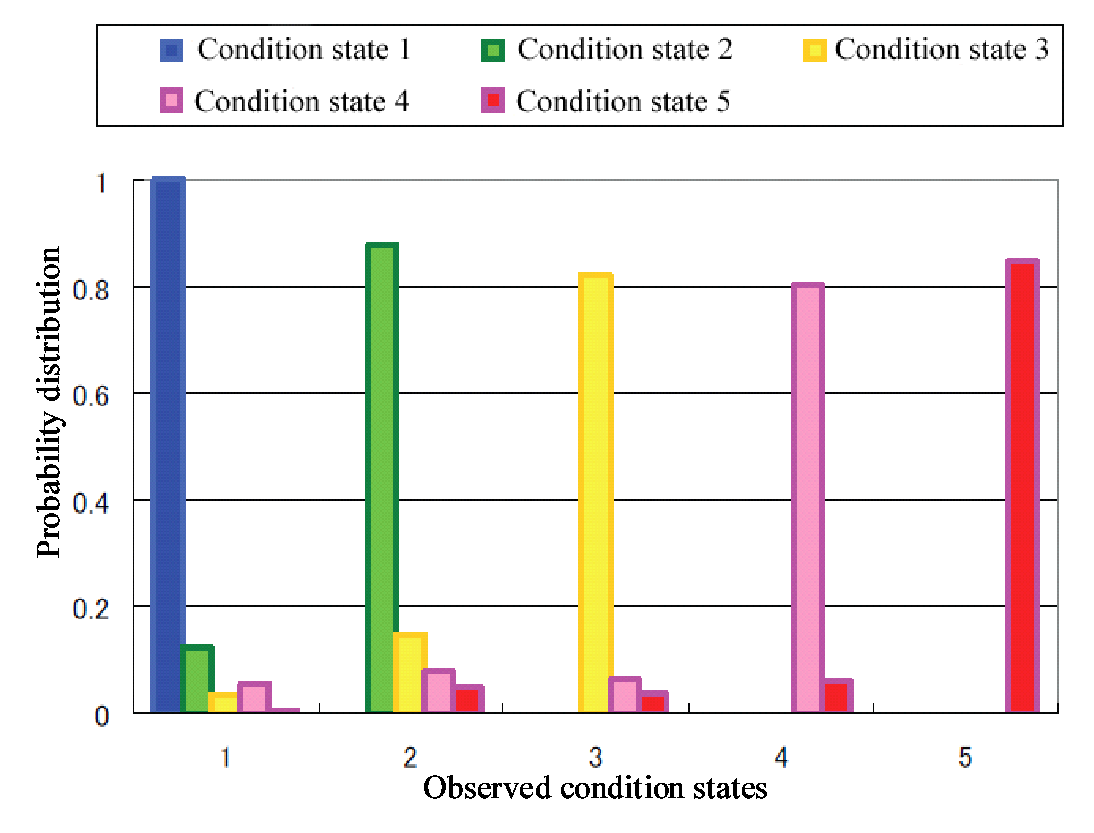
\includegraphics[scale=0.5]{fig45.eps}
\caption{Distribution of Condition State.}
\label{figure45}
\end{center}\end{footnotesize}
\end{figure}
%%%
Based on equations (\ref{hazard1}) and (\ref{17}), the values of the hazard rate and the life expectancy of condition state $i$ can be estimated. The results of estimation are presented in table \ref{table44}. It is highlighted from the table that the life expectancy of condition state $i=1$ is less than $3$ years before entering condition state $i=2$. The average life expectancy of other condition states are from $10$ to $15$ years.
%
\begin{table}
\caption{Life Expectancy of Condition States.}
\label{table44}
\begin{center}
   \vspace{-3mm}
{\small
\begin{tabular}{c|cc}\hline
   Condition states& ~$E[\theta_{il}]$~& $E[RMD_{il}^k]$(year) \\\hline
   1 & ~0.362~ & ~2.762  \\
   2 & ~0.070~ & ~14.286  \\
   3 & ~0.107~ & ~9.346 \\
   4 & ~0.112~ & ~8.929 \\
   \hline
\end{tabular}
}
\end{center}
Note) The values of the hazard rate and the life expectancy are not defined for the absorbing condition state ($i=5$) in the Markov chain model.
\end{table}
%%%%%%%%%%%%%%%%%%%%%
%\subsection{Examining analytical results} \label{sec63}
Table \ref{table45} presents the Markov transition probability matrix, which is estimated by using the hidden Markov model. The properties of the matrix are estimated based on the average hazard rates, which represent the deterioration process of the entire road sections. To compare the impact of traffic volume (TV) on the deterioration process, we categorize the traffic volume into 3 cases and estimated the hazard rates for respective cases. The benchmark case (BM case) refers to a case with use of annual average traffic volume. Whilst, another two cases considered the minimum traffic volumes and maximum traffic volumes respectively. Comparative results of three cases are presented in Figure \ref{fig46}.
%
\begin{table}
\caption{Markov transition probability - by hidden Markov model.}
\label{table45}
\begin{center}
{\small
\begin{tabular}{c|ccccc}\hline
Condition&\multicolumn{5}{|c}{Condition states}\\
States & 1 & 2 & 3 & 4& 5 \\\hline
1 & 0.696  & 0.293 & 0.011 & 0.000& 0.000 \\
2 & 0.0  & 0.932 & 0.064 & 0.003& 0.000 \\
3 & 0.0  & 0.0 & 0.898 & 0.096& 0.006 \\
4 & 0.0  & 0.0 & 0.0 & 0.894& 0.106 \\
5 & 0.0  & 0.0 & 0.0 & 0.0& 1.0 \\\hline
\end{tabular}
}
\end{center}
Note) Interval of transition is one year. 
\end{table}
%
\begin{figure}
\begin{footnotesize}
\begin{center}
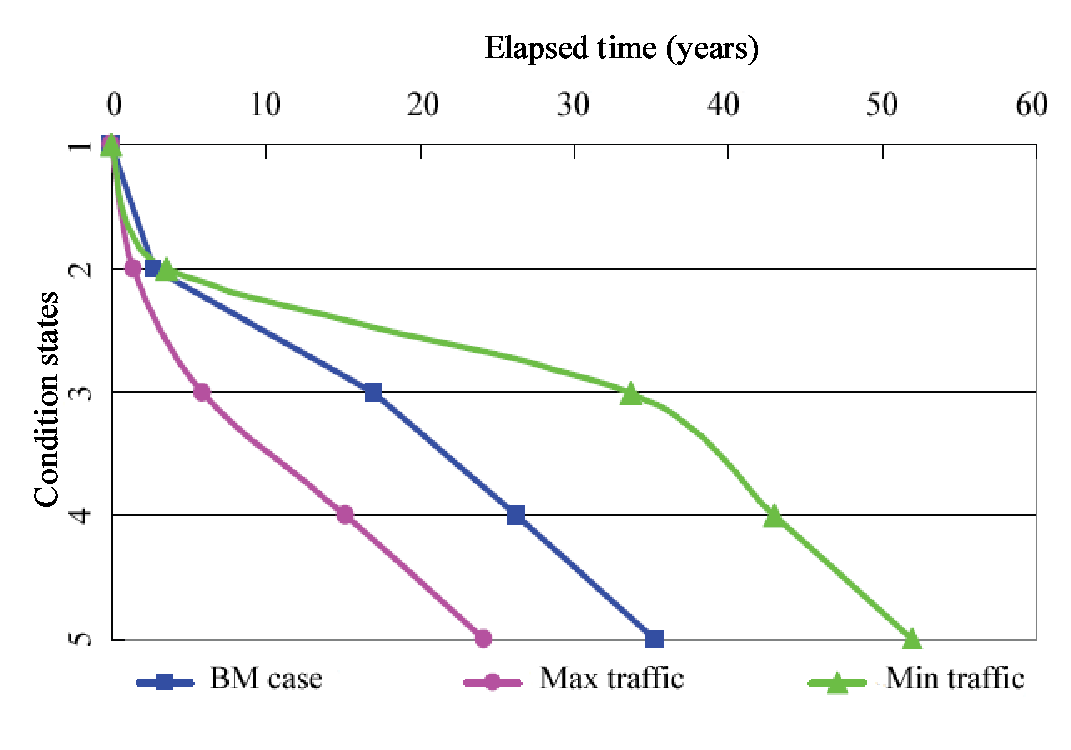
\includegraphics[scale=0.5]{fig46.eps}
\caption{Deterioration curves - traffic volume comparision.}
\label{fig46}
\end{center}
\end{footnotesize}
\end{figure}
%

An appealing conclusion from Fig.\ref{fig46} is that the traffic volume has a high impact on the deterioration process of the road. A sharp decrease in the deterioration curve is observed with the case of maximum traffic volume. In addition, there happen a long delay of the transition from  condition state $2$ to condition state $3$ for all three cases. The deterioration curve of the maximum traffic volume case shows a short life expectancy of condition state $2$. In contrary, the life expectancy of condition state $2$ of the minimum traffic volume case is about $30$ years. The life expectancies of condition state $3$ and $4$ have a similar duration.
%%%%%%%%%%%
\subsection{Measurement errors and estimation bias} \label{463}
To understand the effects of measurement errors on the estimation results, we further examine the estimation of the hidden Markov hazard model on three different databases extracted from the same source of the monitoring data, which is also used in the estimation of the exponential Markov hazard model. The first database (or filtered DB) does not include the samples, which are represented by the dots under the $45^o$ line in figure \ref{fig41}. The second database (corrected DB) is selected based on the first database, with correction of all condition states in the second inspection time appeared to have their values better than that of the first inspection time. The condition states are assumed equal to the condition states of the first inspection time. The third database (reproduced DB) is generated database by using the MCMC simulation, with use of the estimation results in the table \ref{table43}.

A comparative estimation result of the three cases is presented in table \ref{table46}. The values of the parameters under the filtered DB and corrected DB cases are obtained by using the exponential Markov hazard model, whilst, the hidden Markov model is used for estimation with the reproduced DB. The average hazard rates $E[\theta_{il}]$ of three cases are shown in table \ref{table47}.
%%%%

\begin{table*}[t]
\caption{Estimation results for unknown parameters.}
\label{table46}
\begin{center}
\vspace{-3mm}
{\scriptsize
\begin{tabular}{c|cc|cc|cc}\hline
& \multicolumn{2}{|c|}{Filtered DB} & \multicolumn{2}{|c}{Corrected DB}& \multicolumn{2}{|c}{Reproduced DB} \\\cline{2-7}
Condition & Constant term&TV & Constant term&TV& Constant term&TV \\\cline{2-7}
 states & $\beta_{i1}$ & $\beta_{i2}$ & $\beta_{i1}$ & $\beta_{i2}$ & $\beta_{i1}$ & $\beta_{i2}$  \\ \hline
 & 0.247  &  0.325 & 0.214 & 0.362 & 0.270 & 0.415 \\ 
1  & (0.238,0.256) & (0.267,0.378)& (0.205, 0.224) & (0.313,0.421) & (0.257,0.288) &  (0.353,0.477) \\
  & 1.949 & 1.646 & 1.538 & 0.060 & 1.949 & 1.646 \\\hline
 & 0.046 &  0.164 & 0.037 & 0.191 & 0.034 & 0.186\\
2  & (0.043,0.047) & (0.148,0.178)& (0.033,0.038) & (0.173,0.215)& (0.030,0.036) &  (0.170,0.202) \\
  & 1.435 & 1.903 & 1.864 & 0.584 & 1.435 & 1.903 \\\hline
 & 0.139  &  - & 0.127 & - & 0.105 & - \\
3  & (0.131,0.148) & - & (0.120,0.134) & - & (0.099,0.114) &  - \\
  & 0.232 & - & 0.020 & - & 0.232 & - \\\hline
 & 0.163 &  - & 0.131 & - & 0.113 & - \\
4  & (0.150,0.183) & - & (0.118,0.143) & - & (0.101,0.121) &  - \\
  & 0.409 & - & 0.117 & - & 0.409 & - \\\hline
\end{tabular}
}
\end{center}
Note) The values in the blankets show lower and upper bound values of $95\%$ confident interval. The third value in each row is referred to value from Geweke statistical test.
\end{table*}
%%%

A comparison between estimation results of table \ref{table44} and table \ref{table47} revealed that the average hazard rate of the condition state $1$ in the case of using exponential Markov hazard model is lower than that in the case of using the hidden Markov hazard model. On the other hand, the average hazard rates of the condition state $3$ and $4$ are higher in the case of using the exponential Markov hazard model. This findings lead to a conclusion that the over-evaluation on the hazard rates of the condition states $3$ and $4$ are happened in the case of using the filtered DB and the corrected DB. Additional evidence can be realized from looking at the tails of the deterioration curves in the Fig. \ref{fig47}.

%
\begin{table}
\caption{Estimation results for average hazard rates.}
\label{table47}
\begin{center}
{\small
\begin{tabular}{c|ccc}\hline
Condition & Filtered & Corrected & Reproduced\\
States & DB & DB & DB\\\hline
1   &  0.311 & 0.286  & 0.360 \\
2 &  0.079 & 0.075 & 0.069 \\
3   & 0.139 & 0.127 & 0.107\\
4  & 0.163 & 0.131 & 0.112\\\hline
\end{tabular}
}
\end{center}
%Note) Detailed explanation is referred in section \ref{464}
\end{table}
%
%
\begin{figure}
\begin{footnotesize}
\begin{center}
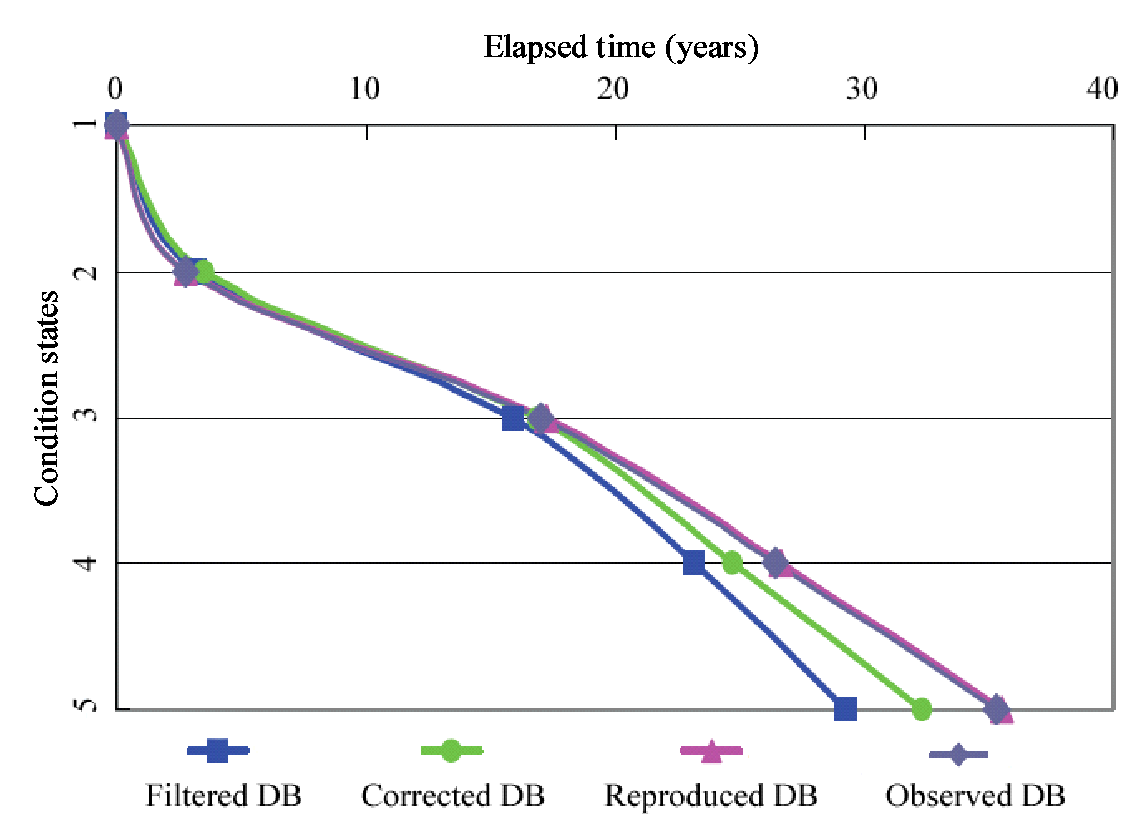
\includegraphics[scale=0.5]{fig47.eps} 
\end{center}
\end{footnotesize}
\caption{Deterioration curves - database comparision.}
\label{fig47}
\end{figure}

The problem of over-estimation on the hazard rates of condition states $i=3,4$ is because of measurement errors. Especially, in the case that $M\&R$ actions had already implemented on a number of the road sections in the past. For example, when the condition state of a road section reachs to $i=3$, mistakes in recording might happen since the corresponding values of rut index are progressing in a negligible manner. This finding suggests future study to develop a methodology to capture the transition pattern of performance indexes like the rut index in an accurate way.
%%%%%%%
\subsection{Simulation of the reproduced database} \label{464}
It is difficult to verify the accuracy of estimation results using the hidden Markov hazard model just with the observed monitoring data alone. To verify the accuracy of the estimation results, it is better to use the obtained estimation results of exponential Markov hazard model to generate the samples through the MCMC simulation. This section details the steps of simulation with the reproduced DB.

The values of parameters presented in the table \ref{table46} under the filtered DB and the corrected DB are used as the inputs of the hidden Markov hazard model. In addition, the traffic volume of large-size car is considered as a main characteristic variable. Moreover, the properties of the Markov transition probability matrix obtained by using the hidden Markov hazard model are used to update the properties of the Markov transition matrix in the exponential Markov hazard model. With this approach, the Markov transition probability $\pi_{ij}(z)$ can be repeatedly updated through equation  and (\ref{4poi}). The so-called ``virtual condition state'' at time $\tau_t^k~(t=1,\cdots,T)$ is randomly generated by using the MCMC simulation in following manners:

%%%%%%%%%%
\begin{itemize}
\item {Firstly, the observed transition probability $\pi_{1j}(z_1^k)$ at time $\tau_1^k$ is considered, with $z_1^k$ as the inspection interval counted from $t=1$. Next, the true condition state $\hat{h}(\tau_1^k)=\hat{i}$ at $\tau_i^k$ is randomly generated}.
\item {Secondly, the transition probability $\pi_{\hat{i}j}(z_2^k)$ is considered. The true condition state in this step alters to be $\hat{h}(\tau_1^k)=\hat{i}$. Next, the true condition state $\hat{h}(\tau_2^k)=\hat{j}$ is randomly generated}.
\item {Finally, the true condition state $\hat{m}(\tau_t^k)$ is randomly generated in a similar algorithm}.
\end{itemize}
%%%%%%%%%%%%%%%%
The distribution of measurement errors (as referred to Fig. \ref{figure45}) and the observed condition states $\hat{m}(\tau_t^k)$ at respective inspection times are considered in the MCMC simulation for generating sampling population. The sampling population is therefore referred as the reproduced database (reproduced DB), and used to estimate the true condition state $\hat{h}(\tau_t^k)~(t=1,\cdots,T)$. Table \ref{table46}, table \ref{table47}, and Fig. \ref{fig47} highlight that the hidden Markov hazard model has produced a better estimation result than that of using the exponential Markov model under the existence of measurement errors.
\section{Conclusion} \label{47}
In this Chapter, we have proposed an innovative analytical approach to forecast the deterioration process of infrastructure through a hidden Markov hazard model. In the model, measurement errors are considered as random variables. Measurement errors are eliminated through the assumption of prior and posterior distribution in Bayesian estimation. Furthermore, Markov Chain Monte Carlo simulation is introduced to generate random sampling population in Bayesian estimation algorithm.

We have presented an empirical study on the Japanese national road system. Estimation results reveal a fact that measurement errors have actually existed in the monitoring data, particularly concerning  condition state $3$ and $4$. Based on the estimation results of using the exponential Markov hazard model, we generate a reproduced database and use it in the hidden Markov hazard model. The estimation results are improved in the case of using the reproduced DB. 

However, we have not discussed several points, which will be considered as topics for extending this study in the future:
%
\begin{itemize}
\item{The empirical study is carried out only on the pavement system. However, this model can be applied for various types of infrastructure. Depending on structural characteristics and the prior knowledge of each infrastructure system, measurement errors can be considered not only as a random variable but also as in the form of a linear function}.
%
\item {The model can be extended if the hazard rate is considered in the form of mixture model. The mixture model can be useful to eliminate the effects of various factors on measurement errors}.
%
\item {Since the estimation results revealed a high risk of having measurement errors with condition state $3$ and $4$ in monitoring and inspection of pavement system, it is suggested that future research should pay attention on finding the reasons causing measurement errors on condition state $3$ and $4$}.
\end{itemize} % Hidden Markov model

% Chapter 1

\chapter{Time-dependent Repair Strategy} % Write in your own chapter title
\label{Chapter5}
\lhead{Chapter 5. \emph{Time-dependent Repair Strategy}} % Write in your own chapter title to set the page header
%%%

%\textbf{Keywords:} Weibull hazard function, optimal renewal interval, pipeline management.
\section{General introduction}
\label{51}
Water pipelines system in a mega city is considered as one of the most important infrastructure system of the city. Major engineering function of the system is for transportation of clean and purified water from treatment and distribution plants to various users including organizations, factories and households. Due to the limitation of land-use and social requirements, in most of the case, pipelines are placed as underground, beneath the pavements, railways and other infrastructures \cite{ahammed97}. In view of the pipeline as underground system, one of the main challenging tasks for engineer is to understand the deterioration behaviors such as: leakage occurrence, corrosion progress, wall of pipe over the time, external impact pressure, etc. This query is indeed necessary in order to efficiently operate the system so as to provide the best quality and sufficient volume of water for the city dwellers.

The main physical deteriorate problem of pipeline is corrosion resulting from many influential factors such as: internal fluid pressure, material elastic modulus, longitudinal stress, coating type, soil impact, external load and many others. Evidently, corrosion over the operation time undoubtedly and slowly leads to leakage and break of pipe. In fact, leakage occurrence and break of pipeline system in a mega city due to natural corrosive process and external factors have been well-documented as a widespread problem. As a sequent, water supply companies are asked to bear huge losses due to pressure head losses, high repair and penalty cost in case of damage occurrences. Additionally, in view of social losses, a great amount of money needs to be allocated for other potential adverse consequences such as flooding, fast deterioration of roads, road congestion, closing of business and shopping centers and other indirect expenses \cite{deb03}.

As the matter of course, data on actual performance of pipelines over the years is often absence because of its complexity and high cost in inspection. For example, the visual inspection requires excavation of existing upper structures, which therefore prevents other services from normal operation. Moreover, in the case of regular maintenance or immediate repair, the involved costs are often claimed to be considerably high. Thus, in an economical view, managers prefer to select the option of renewing the pipeline to repair alternative because the overall cost in fact receiving very small variation from material cost itself. This ideal consequently leads to the demand of determining the optimal renewal time based on the principle of minimizing the overall life cycle cost (LCC).

The determination for renewal duration is in close link not only to the overall cost but also to the durability of pipeline. Naturally, high durability pipeline is often turning to have longer optimal renewal time. In the situation of having various types of pipelines, selecting the best one that satisfies both high durability and minimum LCC requires an appropriate benchmarking study. In consideration of benchmarking, suffice to say that only when the optimal renewal duration of each pipeline type is determined, a selection of the most appropriate technology of pipelines would be feasible.

This study aims to formulating an optimal renewal model of pipeline system. Pipeline systems are subjectively categorized into different types according to the characteristics of construction materials. Each type of pipeline is further grouped by differences in diameter. Weibull hazard function is employed to address the elapsed time of each pipeline measuring from its buried time. The physical impact factors are in form of risk factor with a certain probability or range. Each impact factor results in a particular risk level and is integrated into hazard function. Expected life cycle cost considers both direct replacement cost and indirect social cost. 

The model is used for forecasting the deterioration of pipelines and determining the optimal renewal time that offers the minimum expected life cycle cost of each pipeline. The optimal types of pipeline could be identified as the best alternative for future replacement. The presumption of model is presented in the second section. The third section discusses the deterioration process of pipeline system. The best renewal interval model is portrayed in the fourth section. Empirical application to the water distribution network of Osaka city, which was established in 1895, is examined and explained in the fifth section.
%%%%%%%%%%%%%%%%%%
%\section{General Background}
%\label{52}
%%%%%%%%%%%%%%%%%%%%%%%%%%%%%%%%%%%%%%%%%%%%%%%%555
%%%%%%%%%%%%%%%%%%%%%%%%%%%%%%%%%%%%%%%%%%%%%%%%%%%
\section{Pre-assumption of the Model}
\label{53}
%%%%%%%%%%%%%%%%%%%%%%%%%%%%%%%%%%%%%%%%%%%%%%%%%%%
Suffice to say that the demand for pipeline replacement of water distribution network would not become a heavy burden if abundant resource were allocated annually. However, the scarcity of resources bring up to the managers a question of when, how and what to do for the entire network and for individual pipeline. Thus, for managerial purposes, it ought to be important not only to estimate the optimal renewal time but also the most appropriate substitute type of pipeline for present and future replacement. 

In pipeline system, there are two distinguish level of deterioration, denoting as $E_i (i=1,2)$. Level $E_1$ reflects the healthy condition in good level. Whilst, level $E_2$ denotes the pipeline is under leakage, damage or destruction. Anytime when the condition level $E_2$ is detected, the damaged pipeline will be replaced to a new one immediately. In the concurrence of incident, especially in the mega cities, tap water will spill over the surface of the road, or shopping center that lead to the social damage such as: traffic congestion, flooding and downtime of office, business center in the downtown. By substituting the old pipeline proactively, the risk of undertaking the incident could be mitigated. This is under the control and decision of Water Supply Company. As the matter of course, the substitution of pipeline demands an increase in the replacement cost. It is therefore important to harmonize the trade-off situation by introducing the optimal renewal interval with respect to the summation of total social cost and renewal cost as a whole.
\section{Deterioration Process}
\label{54}
In hazard analysis, the deterioration of element is subjected to follow a stochastic process \cite{lancaster90}. For pipeline, as previously mentioned, two condition level $E_1, E_2$ are defined. Figure \ref{fig51} describes the deterioration process of pipeline and choice of renewal. In the case of renewal, the condition state from $E_2$ must be changed into $E_1$ as for new pipeline and the pipeline resuming its normal performance condition. The renewal is carried out at alternative time $t_k$ $(k=0,1,2,...)$. In this way, the next renewal time is denoted as $t=t_0+\tau$, where $\tau$ indicating the elapsed time. The life span of the pipeline is expressed by a random variable $\zeta$. The probability distribution and probability density function of the failure occurrence are $F(\zeta)$ and $f(\zeta)$ respectively. The domain of the random variable $\zeta$ is $[0,\infty]$. The living probability (hereafter named as survival probability) expressed by survival function $\tilde{F}(\tau)$ can be defined according to the value of failure probability $F(\tau)$ in the following equation:
\begin{figure}[t]
\begin{center}
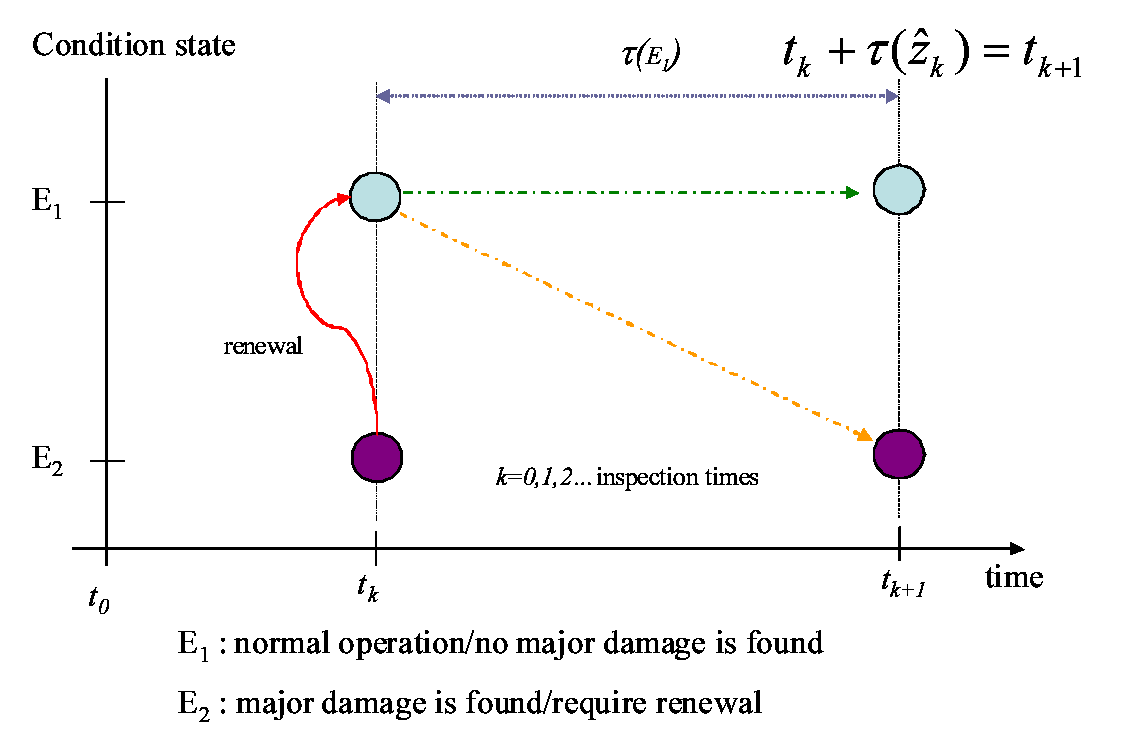
\includegraphics[scale=0.5]{fig51.eps}
\end{center}
\caption{Deterioration and Renewal Choice.}
\label{fig51} 
\end{figure}
\begin{eqnarray}
&& \tilde{F}(\tau) = 1 - F(\tau). \label{funcbF5}
\end{eqnarray}
The probability, at which the pipeline performs in good shape until time $\tau$ and break down for the first time during an interval of $\tau+\Delta\tau$ can be regarded as hazard rate and expressed in the following equation:
\begin{eqnarray}
&& \lambda_i(\tau) \Delta \tau = \frac{f(\tau)\Delta \tau}{\tilde{F}(\tau)}, \label{riskbF5}
\end{eqnarray}
where $\lambda(\tau)$ is the hazard function of the pipeline. In reality, the breakdown probability depends largely on the elapsed time of pipeline since its construction time. Thus, the hazard function should take into account the working duration of the pipelines. In another word, the memory of the system should be inherited. Weibull hazard function is satisfied in addressing the deterioration process:
\begin{eqnarray}
&& \lambda(\tau)= \alpha m \tau^{m-1}, \label{weibul}
\end{eqnarray}
where $\alpha$ is the parameter expressing the arrival density of the pipeline, and $m$ is the acceleration or shape parameter. The probability density function $f(\tau)$ and survival function $\tilde{F}(\tau)$ in the form of Weibull hazard function can be further expressed in equation (\ref{pdf}) and (\ref{survival}):
\begin{eqnarray}
&& f(\tau)=\alpha m\tau^{m-1}\exp(-\alpha \tau^m), \label{pdf} \\
&& \tilde{F}(\tau)=\exp(-\alpha \tau^m). \label{survival}
\end{eqnarray}
\section{Risk Factors and Estimation Approach for Weibull Parameters}
\label{55}
\subsection{Risk Factor and Covariates}
\label{551}
\subsubsection{Risk Factor}
\label{5511}
The corrosion process of pipeline is affected by many internal and external factors. As earlier mentioned, the influential factors include material yield stress, length, radius, pipe wall thickness, traffic load, unit soil weight, thermal expansion coefficient, internal fluid pressure and many others. These factors should be considered as either deterministic or random variables with specific mean and variance depending on the availability of gathered data and information. Evidently, these factors are proportionally contribute to the deterioration level with difference variation \cite{ahammed95,ahammed97}. It is therefore, it is understandable to propose an integrated risk factor $\kappa$ in form of probability value. This risk factor receives different value in the case of different mega city, different type of water distribution system, materials and so on and so fourth. Estimation of risk factor can be retrieved from several physical models. Further expression of hazard function whereby considering the risk factor $\kappa$ is as follow:
\begin{eqnarray}
&& \lambda(\tau)= \kappa \alpha m \tau^{m-1}. \label{weibul1}
\end{eqnarray}
The probability density function $f(\tau)$ in (\ref{pdf}) and survival function in (\ref{survival}) $\tilde{F}(\tau)$ are further expressed as
\begin{eqnarray}
&& f(\tau)=\kappa \alpha m\tau^{m-1}\exp(-\kappa \alpha \tau^m), \label{pdf1} \\
&& \tilde{F}(\tau)=\exp(-\kappa \alpha \tau^m). \label{survival1}
\end{eqnarray}
A further notice in the case of using the risk factor is that $\kappa$ should be used for respective record available in the data set.
\subsubsection{Covariates}
\label{5512}
Beside the risk factor, another popular approach in addressing the impacts and correlations of characteristic variables (or covariates) is to consider location parameter $\alpha$ in additive form of covariates:
\begin{eqnarray}
\alpha  = \sum\limits_{i = 1}^M {\beta _i x_i \rm{  \hspace{2mm}   (i = 1,}}...{\rm{,M)}}, \label{covariate}
\end{eqnarray}
where $m$ is total number of covariates and the value of first covariate equals to 1 as a constant value. Depending the availability of database, numbers of covariates are selected in to numerical calculation.
\subsection{Estimation Approach for Weibull Parameter}
\label{552}
It is assumed that the total number of recorded data is $S$, which is relatively equivalent to entire length of the pipelines system. In which, each record refers particularly for $s$ $(s=1,...,S)$ unit of length (possibly in meter or kilometer). This type of separation is often found for the convenience of management of each city. Equations (\ref{pdf}) and (\ref{survival}) are thus in the following formula:
\begin{eqnarray}
&& f(t_s)=\alpha mt_s^{m-1}\exp(-\alpha t_s^m), \\
&& \tilde{F}(t_s)=\exp(-\alpha t_s^m).
\end{eqnarray}
%%%%%%%%%%%%%%%%%%%
Deterioration of section $s$ is considered as mutually independent from other part of the pipelines system. For this reason, the simultaneous probability density of the deterioration is expressed in the following likelihood function: 
%%%%%%%%%%%%%%%%%%%%%
\begin{eqnarray}
\begin{array}{l}
 {\cal L} (\alpha , m: t_s) = \prod\limits_s^S {\left\{ {\bar F(t_s^m )} \right\}^{(1 - \delta _s )} \left\{ {f(t_s^m )} \right\}^{\delta _s } }    \\
= \prod\limits_s^S {\left\{ {\exp ( - \alpha t_s^m )} \right\}^{(1 - \delta _s )} \left\{ {\alpha mt_s^{m - 1} \exp ( -  \alpha t_s^m )} \right\}^{\delta _s } } , \label{eq11}
 \end{array}
\end{eqnarray}
where $\delta_s$ is dummy variable receiving its value of $1$ when leakage was encountered and $0$ otherwise. For ease of mathematical manipulation, logarithm for both sides of equation (\ref{eq11}) is referred. Thus, following equation is additional named as log-likelihood function:
\begin{eqnarray}
&&\ln {\cal L} (\alpha, m: t_s )=  
\sum\limits_s^S {\left[ \begin{array}{l}
 (1 - \delta _s )( - \alpha t_s^m ) \\ 
  + \delta _s \left\{ {\ln \alpha  + \ln m + (m - 1)\ln t_s  - \alpha t_s^m } \right\} \\ 
 \end{array} \right]} .\label{weilike}
\end{eqnarray}
In order to obtain the two parameter $\alpha$ and $m$, the maximum likelihood estimation method is used. The estimator of parameter value $\theta$ which maximizes the logarithmic likelihood function (\ref{weilike}) is given as $\hat\theta =(\hat \theta _1 ,\hat\theta _2)$ ($\theta _1 =\alpha, \theta _2 =m $) and must simultaneously satisfies following condition:
\begin{eqnarray}
\frac{{\partial \ln {\cal L} (\Xi ,\hat \theta )}}{{\partial \theta _i }} = 0,{\rm{      }}(i = 1,2) .
\end{eqnarray}
Furthermore, the estimated value $\sum {\hat \theta }$ of the asymptotic covariance matrix of the parameter can be expressed as follow:
\begin{eqnarray}
\sum\limits_{}^ \wedge  {(\hat \theta ) = \left[ {\frac{{\partial \ln {\cal L} (\Xi ,\theta )}}{{\partial \theta \partial \theta^{'} }}} \right]} ^{ - 1} . \label{fisher}
\end{eqnarray}
%%%%%%%%%
The optimal value of $\hat\theta =(\hat \theta _1 ,\hat\theta _2)$ are then estimated by applying numerical iterative procedure such as Newton method for simultaneous equation (\ref{fisher}) of 2 dimensions. This study employs Newton-Rhapson method. The statistical $t$-test is calculated by use of covariance matrix value $\sum {\hat \theta }$.
%%%%%%%%%%%%%%%%%%%%%%%%%%%%%%%%%%%%%%%%%
\section{Formulation of the Optimal Renewal Interval Model}
\label{56}
The occurrence of the incident results in an amount of social cost, which is assumed to be a constant number $C$. The expected social cost $EC(z)$ is estimated by use of the predetermined interval of renewal $z$. Thus, its value is followed the probabilistic manner via probability density function $f(\tau)$ defined in equation (\ref{pdf}). Over the continuous time, counting from the buried time or the previous renewal time, the expected social cost would be in the integral form as expressed in the following equation:
\begin{eqnarray}
&& EC(z)=\int_0^{z} C f(t)\exp(-\rho t)dt. \label{socialcost}
\end{eqnarray}
The co-efficient $\rho$ is discounted rate of money over the interval $z$. On the other hand, another constant amount of money denoted as $I$ is spent for renewal activities, which is subjected to either occurrence of incident at time $\tau$ or the age of pipeline reaching to time $z$. It is therefore important to note that the renewal cost, when the age of pipeline becomes $z$, must take the survival probability $\tilde{F}(\tau)$ into its calculation. Consequently, the present discounted cost of the next pre-determined renewal time $EL(z)$ can be expressed in the following form:
\begin{eqnarray}
EL(z)=\int_0^{z} I f(t)\exp(-\rho t)dt +  \tilde{F}(z)I \exp(-\rho z). \label{totalcost}
\end{eqnarray}
The expected life cycle cost after the next renewal time is evaluated as net present value of social costs, renewal costs. As the social and renewal cost are in fixed values, the expected LCC alters to be equal for every renewal times. In another word, expected LCC at next renewal time is equal to the expected LCC estimated at the present renewal. The expected LCC, denoted as $J(0:z)$, can be regulated through the regression estimation shown in equation (\ref{han}):
\begin{eqnarray}
&& J(0:z)= \int_0^{z} f(t)\{c+I+J(0:z)\} \exp(-\rho t)dt  \nonumber \\
&& \hspace{10mm} + \tilde{F}(z)\{I+J(0:z)\} \exp(-\rho z).  \label{han}
\end{eqnarray}
The following two functions $\Gamma(z)$ and $\Lambda(z)$ are defined:
\begin{eqnarray}
&& \Gamma(z)=\int_0^{z} f(t)\exp(-\rho t)dt 
 = \int_0^z  \alpha m\tau^{m-1}\exp(- \alpha \tau^m-\rho t)dt, \label{gamma5}\\
&& \Lambda(z)= \tilde{F}(z) \exp(-\rho z)
  =\exp(- \alpha z^m-\rho z) . \label{alpha}
\end{eqnarray}
Substituting equations (\ref{gamma5}) and (\ref{alpha}) into equation (\ref{han}), the following explicit form for the expected LCC is obtained:
\begin{eqnarray}
&& J(0:z)= \frac{(c+I)\Gamma(z)+I \Lambda(z)}{1-\Gamma(z)-\Lambda(z)} .\label{lifecycle}
\end{eqnarray}
The optimal value function $\Phi(0)$ can be expressed as the minimum expected LCC evaluated at the initial time:
\begin{eqnarray}
&& \Phi(0)=\min_{z}\{ J(0:z) \}.\label{imp}
\end{eqnarray}
The estimation for the optimal interval $z^*$ from equation (\ref{lifecycle}) can be handled by solving the optimization condition of the first derivative as expressed in the following equation:
\begin{eqnarray}
&& \frac{dJ(0:z)}{dz}=\frac{ \psi(z)}{\{1-\gamma(z)-\Lambda(z)\}^2 }=0, \\
\text{where}\nonumber \\
&& \psi(z)=(C+I)\Gamma^\prime(z)+I\Lambda^\prime(z)+C\{\Lambda(z)^\prime\Gamma(z)
 -\Gamma^\prime(z)\Lambda(z)\},
\end{eqnarray}
$\Gamma(z)^\prime=d\Gamma(z)/dz$ and $\Lambda(z) ^\prime=d\Lambda(z)/dz$. Obtaining the value of optimal interval $z^*$ requires to solve the equation $\psi(z)=0$. Another numerical approach to solve equation (\ref{lifecycle}) is further explained in appendix A.
%%%%%%%%%%%%%%%%%%%%%%%%%%%%%%%%%%%%%%%%%%%%%%%%%%%%%%%%
\section{Optimal Renewal Interval and Technology Innovation}
\label{57}
The water distribution network composes of many different types of pipes. Thanks to the technology innovation in pipe's materials, many new and better quality types of pipe have been introduced. As a matter of course, along the time, pipelines made from outdated materials are no longer in production. The aging pipelines are deeming to be substituted by better quality pipes. It is assumed that the network composes of type $i$ $(i=1,...,N)$, which is available in the stock ($N$ is total number of type $i$). On the other hand, there exists pipes of old fashion type $j$ $(j=1,...,M)$ ($M$ is the total number of old type). The selection of pipe according to its type for renewal activities can be described in two subsequent steps as follows:
%%%%%%%%%%%%%%%%%%%%%%%%%%%%%%%%%%%%%%%%%%%%%%%
\subsection{Step 1-Selection of Best Type of Pipe}
\label{571}
The optimization approach expressed in equation (\ref{lifecycle}) and (\ref{imp}) warrants the estimation for the best interval renewal time for each type $i$ $(i=1,...,N)$ of pipelines. From equation (\ref{han}), the following equation is regarded as the expected LCC for type $i$:
\begin{eqnarray}
&& J_i(0:z_i)= \int_0^{z_i} f_i(t)\{c+I_i+J_i(0:z_i)\} \exp(-\rho t)dt  \nonumber \\
&& \hspace{10mm} + \tilde{F}_i(z_i)\{I+J_i(0:z_i)\} \exp(-\rho z_i).  \label{han1}
\end{eqnarray}
The best type $i^*$ is the one meeting the minimum expected LCC condition among $N$ types:
\begin{eqnarray}
&& i^\ast=\mbox{arg} \min_{i}\{J_i(0:z_i):i=1,\cdots,N\}. \label{16}
\end{eqnarray}
The sign $\mbox{arg}\min_{i}$ denotes the minimization searching for the function in the parenthesis with respect to $i$. The best type $i^*$ evaluated from condition of equation (\ref{16}) would become optimal type for replacement of old types of pipelines in the entire water distribution network.
%%%%%%%%%%%%%%%%%%%%%%%%%%%%%%%%%%%%%%%%%%%%%%%
\subsection{Step 2-Replacement for Old Type Pipeline}
\label{572}
In regard to replacement rules, the expected life cycle $\tilde{J}_j^{i^\ast} (z_j:\tau_j)$ cost calculated for the old type $j$ of pipe by using the optimal type $i^*$ acquired from Step 1 and after interval time $z_j$ become the net present value expressed in the following equation:
\begin{eqnarray}
&& \tilde{J}_j^{i^\ast}(z_j:\tau_j)
 =\int_0^{z_j} f_j(t_j|\tau_j)\{c+I_{i^\ast}+J_{i^\ast}(0:z_{i^\ast})\} \exp(-\rho t_j)dt_j  \nonumber \\
&& + \tilde{F}_j(z_j|\tau_j)\{I+J_{i^\ast}(0:z_{i^\ast})\} \exp(-\rho z_{i^\ast}) . \label{han2}
\end{eqnarray}
The problem of seeking for the optimal renewal time $z_j^\ast(\tau_j)$ for old type $j$ with elapsed time $\tau$ is by solving the optimization condition in the following expression:
\begin{eqnarray}
&& z_j^\ast=\arg \min_{z_j} \{\tilde{J}_j^{i^\ast}(z_j:\tau_j)\} .\label{sa}
\end{eqnarray}
%%%%%%%%%%%%%%%%%%%%%%%%%%%%%%%%%%%%%%%%%%%%%%
%%%%%%%%%%%%%%%%%%%%%%%%%%%%%%%%%%%%%%%%%%%%%%
The so called \textit{"Switching ratio $\Theta$" }, inferring the rate of renewal by using the new type of pipelines over the old types, is expected to become an important indicator for replacement planning. Definition of the rate is the ratio of $z^*_j$ over $z^*_i$:
%%%
\begin{eqnarray}
&& \Theta = \dfrac{z^*_j}{z^*_i} .\label{swratio}
\end{eqnarray}
%%%%
\section{Average Cost Estimation.}
The application of average life cycle cost analysis has been widely recommended for economic evaluation of public infrastructure, Especially, for infrastructure with its long service life. This is due to the fact that, over the years, discount rate $\rho$ often exerts a high fluctuation in its value. In order to minimize the negative impact on analysis from such high fluctuation of discount rate, \cite{kobaevarg} has proved the benefit of using average cost analysis.

The case when life cycle cost is applicable is in line with the case when the denominator of the expression \ref{lifecycle} becomes $0$ in the limit of which discount rate $\rho=0$. However, when the value of denominator equals to $0$, the equation can not be solvable. In consideration average cost over the service life, we apply estimation for average cost of pipeline type $i~(i=1,\cdots,N)$ by following equation:
\begin{eqnarray}
&& AC_i(z)=\frac{\int_0^{z} (c+I_i) f_i(t) dt  +  \tilde{F}_i(z)I_i}{z} .\label{avelcc}
\end{eqnarray}
The optimal renewal time $z_i^\ast$ for pipeline type $i$ can be estimated by solving the minimum condition of equation \ref{avelcc}:
\begin{eqnarray}
&& \min_{z}\{ AC_i(z) \}.\label{iimp}
\end{eqnarray}
Among $N$ number of type $i$, again, it is possible to select the best type $i^\ast$ in view of least life cycle cost:
\begin{eqnarray}
&& i^\ast=\mbox{arg} \min_{i}\{ AC_i(z_i^\ast):i=1,\cdots,N\}.
\end{eqnarray}
Eventually, it is possible to define the average cost if the best pipeline type $i^\ast$ is used to replace the old type of pipeline $j$. And thus, it is necessary to define the renewal period $z_j$ in case of renewal with best possible pipeline technology:
\begin{eqnarray}
&& \hspace{-5mm} \overline{AC}_j^{i^\ast}(z_j)
  =\frac{\int_0^{z_j} f_j(t_j|\tau_j)(c+I_{i^\ast}) dt_j  + \tilde{F}_j(z_j|\tau_j)I_{i^\ast} }{z_j} .\label{han11}
\end{eqnarray}
$\tilde{F}_j(t_j|\tau_j)$ is the probability, to which, leakage or breakdown do not occur during time $t_j$ and continue the same condition state until time $\tau_j$. If the best pipeline type $i^\ast$ now is used, the average cost $AC_{i^\ast}(z_i^\ast)$ is generated. In addition, the accumulative additional cost generated by continuously using the old pipeline for the $z_j$ period can be determined:
\begin{eqnarray}
&& \overline{CAC}_j^{i^\ast}(z_j)= \{\overline{AC}_j^{i^\ast}(z_j)-AC_{i^\ast}(z_i^\ast)\}z_j.
\end{eqnarray}
In the end, the best renewal time $z_j^\ast(\tau_j)$ for pipeline type $j$ can be easily estimated by choosing the renewal time satisfying the minimum condition: 
\begin{eqnarray}
&& z_j^\ast=\arg \min_{z_j} \{\overline{CAC}_j^{i^\ast}(z_j)\}. \label{ssa}
\end{eqnarray}
\section{Empirical Study}
\label{58}
\subsection{Overview of Empirical Study}
\label{581}
%%%%%%%%%%%%%%%%%%%%%%%%%%%%%%%%%%%%%%%%%%%%%%
The water distribution network of Osaka city was mainly constructed during the periods of 1950s and 1960s. The network has undergone nice times of expansion to meet the need of the city \cite{osaka}. The total length of conduct, transmission and distribution pipe is approximately 5,000 km. Since 1965, the City has systematically upgraded the distribution system by installing new pipes, renewing aged ones, lining all pipes, etc. As a result, a network of distribution pipes in the city has been satisfactorily established, eliminating insufficient supply and low water pressure supply areas. To date, the subsequent maintenance and renewal activities have been so far implemented for over $4,000$ km, requiring about more than $390$ billion Japanese Yen.

Technically, the entire water distribution system composes of four distinguish types, which belongs to class A, C, F and FL. The three types C, F and FL are the old cast iron types, which were buried in the early period. At the present, those pipes are no longer in the manufacturing. As the matter of course, the social cost $C$, direct cost $I$ and discounted rate $\rho$ plays a center role in establishing the optimal renewal years as well as the expected LCC, sensitivity analysis with focus on the ranges are drawn for respective types of pipelines. However, for ease of estimation, benchmark case was selected with social cost $C=5$ million Yen, $I =1$ million Yen and $\rho=0.04$.%%%%%%%%%%%%%%%%%%%%%%%%%%%%%%%%%%%%%%%%%%%%%%
\subsection{Estimation Results}
\label{582}
\subsubsection{Weibull's parameters and survival probability}
\label{5821}
%%%%%%%%%%%%%%%%%%%%%%%%%%%%%%%%%%%%%%%%%%%%%%
The parameters $\alpha$ and $m$ of embedded hazard function are estimated by maximum likelihood method with historical sectional records for each type of pipeline. Values of $\alpha$ and $m$ are then verified with significant degree of $t$ test values. Table \ref{table51} presents the results of estimation for two comparative cases. The first case refers as case, to which explanatory variables were excluded from estimation. Second case were when the effective length as characteristic variable was considered in estimation. Regarding the second case, as presented in the table, unknown parameter $\beta_1$ is referred to a constant term with its value of $1$ for characteristic variable $x_1$. Unknown parameter $\beta_2$ is referred to the effective length of pipeline system. 

In this study, other characteristic variables, which reflect the influence of outer and inner rutness, soil unit weight, top traffic volume, etc, were neglected due to its small impact or data unavaibility. The value in blankets in Table \ref{table51} refers to value of statistical $t-test$. It is realized from $t-test$ value that effective length of pipeline somehow effect the deterioration process. This conclusion is further understandable from comparison of AIC \footnote{AIC-Akaike Information Criteria was developed by Hirotsugu Akaike, a Japanese statistician, in 1971. The AIC is not test on the model in the sense of hypothesis testing, rather it is a tool for model selection.} (Akaike Information Criteria)  \cite{akaike} values. AIC values of case with considering effective length of pipeline are lower than the case without that covariate in estimation (AIC values are shown in the last line of each row in Table \ref{table51}).
%
\begin{table}[t]
\caption{Estimation Results for the Parameters of Weibull Functions-Types}
\label{table51}
{\small
\begin{center}
\begin{tabular}{l|ll|lll}
\hline
\multicolumn{1}{c|}{Pipeline} & \multicolumn{2}{c|}{Without covariate} & \multicolumn{3}{c}{With covariate} \\ 
\multicolumn{1}{c|}{types} & \multicolumn{1}{c}{$\alpha$} & \multicolumn{1}{c|}{m} & \multicolumn{1}{c}{$\beta_1$} & \multicolumn{1}{c}{$\beta_2$} & \multicolumn{1}{c}{m} \\ 
\hline
\multicolumn{1}{c|}{C} & \multicolumn{1}{c}{1.11E-05} & \multicolumn{1}{c|}{2.496} & \multicolumn{1}{c}{2.51E-06} & \multicolumn{1}{c}{1.49E-04} & \multicolumn{1}{c}{2.484} \\ 
\multicolumn{1}{c|}{} & \multicolumn{1}{c}{(28.528)} & \multicolumn{1}{c|}{(30.275)} & \multicolumn{1}{c}{(6.402)} & \multicolumn{1}{c}{(19.666)} & \multicolumn{1}{c}{(34.909)} \\ 
\multicolumn{1}{c|}{} & \multicolumn{2}{c|}{5053.724 } & \multicolumn{3}{c}{4,031.920 } \\ 
\hline
\multicolumn{1}{c|}{F} & \multicolumn{1}{c}{2.55E-05} & \multicolumn{1}{c|}{2.293} & \multicolumn{1}{c}{4.92E-06} & \multicolumn{1}{c}{3.25E-04} & \multicolumn{1}{c}{2.288} \\ 
\multicolumn{1}{c|}{} & \multicolumn{1}{c}{(46.256)} & \multicolumn{1}{c|}{(48.825)} & \multicolumn{1}{c}{(9.337)} & \multicolumn{1}{c}{(32.944)} & \multicolumn{1}{c}{(56.613)} \\ 
\multicolumn{1}{c|}{} & \multicolumn{2}{c|}{13,523.840 } & \multicolumn{3}{c}{11,154.640 } \\ 
\hline
\multicolumn{1}{c|}{FL} & \multicolumn{1}{c}{1.81E-05} & \multicolumn{1}{c|}{2.400} & \multicolumn{1}{c}{6.73E-06} & \multicolumn{1}{c}{1.22E-04} & \multicolumn{1}{c}{2.391} \\ 
\multicolumn{1}{c|}{} & \multicolumn{1}{c}{(14.537)} & \multicolumn{1}{c|}{(15.432)} & \multicolumn{1}{c}{(4.375)} & \multicolumn{1}{c}{(7.365)} & \multicolumn{1}{c}{(17.790)} \\ 
\multicolumn{1}{c|}{} & \multicolumn{2}{c|}{1,331.980 } & \multicolumn{3}{c}{1,114.080 } \\ 
\hline
\multicolumn{1}{c|}{A} & \multicolumn{1}{c}{8.87E-05} & \multicolumn{1}{c|}{1.907} & \multicolumn{1}{c}{8.27E-06} & \multicolumn{1}{c}{4.18E-04} & \multicolumn{1}{c}{2.144} \\ 
\multicolumn{1}{c|}{} & \multicolumn{1}{c}{(29.416)} & \multicolumn{1}{c|}{(31.380)} & \multicolumn{1}{c}{(10.117)} & \multicolumn{1}{c}{(26.642)} & \multicolumn{1}{c}{(35.865)} \\ 
\multicolumn{1}{c|}{} & \multicolumn{2}{c|}{6,654.540 } & \multicolumn{3}{c}{5,588.270 } \\ 
\hline
\end{tabular}
\end{center}
}
{\small Note) Value in the blanket $(-)$ are stasitical t-test. Values in the last row of each type are $AIC$ values.}
\end{table}%[t]
%

%Further to the value of $t-value$ for statistical test, Akaike Information Criteria (AIC) test is highly recommended to have more comprehensive understanding on the correlation of model's parameters \cite{akaike}. Formula for AIC is as follows.
%\begin{eqnarray}
%&& AIC = -2*ln(likelihood)+2*K \label{aic}
%\end{eqnarray}
%where $K$ is the number of parameters in the model. As can be seen from Table 2, the ratios of important weight $w_i$ of case 3 and case 4 receive significant small. This proves the fact that their correlation between these two factors can be neglected. From $t-value$ and AIC value, confidently to say, omission of effective length and rut is acceptable in model's calculation. However, other factors such as traffic volume above the pipelines, unit weight of soil, various type of pressure should be recommended as covariates only if the concerning data are available.
However, as can be proved from Figure \ref{fig52}, Figure \ref{fig53} and Figure \ref{fig54}, the difference in decrease of survival probability over the years are not significant for both cases of pipeline type C, F and FL. A considerable variation between two survival probability curve is realized only for pipeline type A from Figure \ref{fig55}. Since the largest sampling population has been accumulated for pipeline type A (about more than 15,000 data), it can be concluded that, the impact of effective pipeline length has tendency to increase with the larger size of sampling population. 

\begin{figure}[t]
\begin{center}
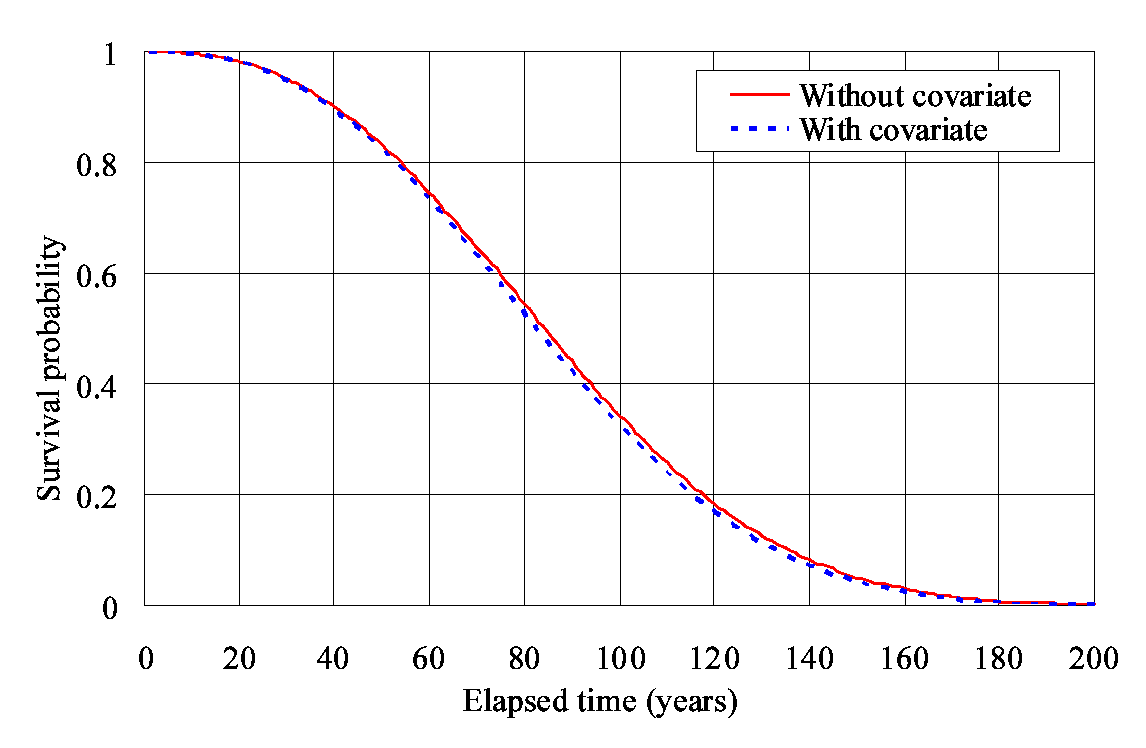
\includegraphics[scale=0.5]{fig52} 
\end{center}
\caption{Survival Probabilities of Type C With and Without Covariates.}
\label{fig52} 
\end{figure}
%
\begin{figure}[t]
\begin{center}
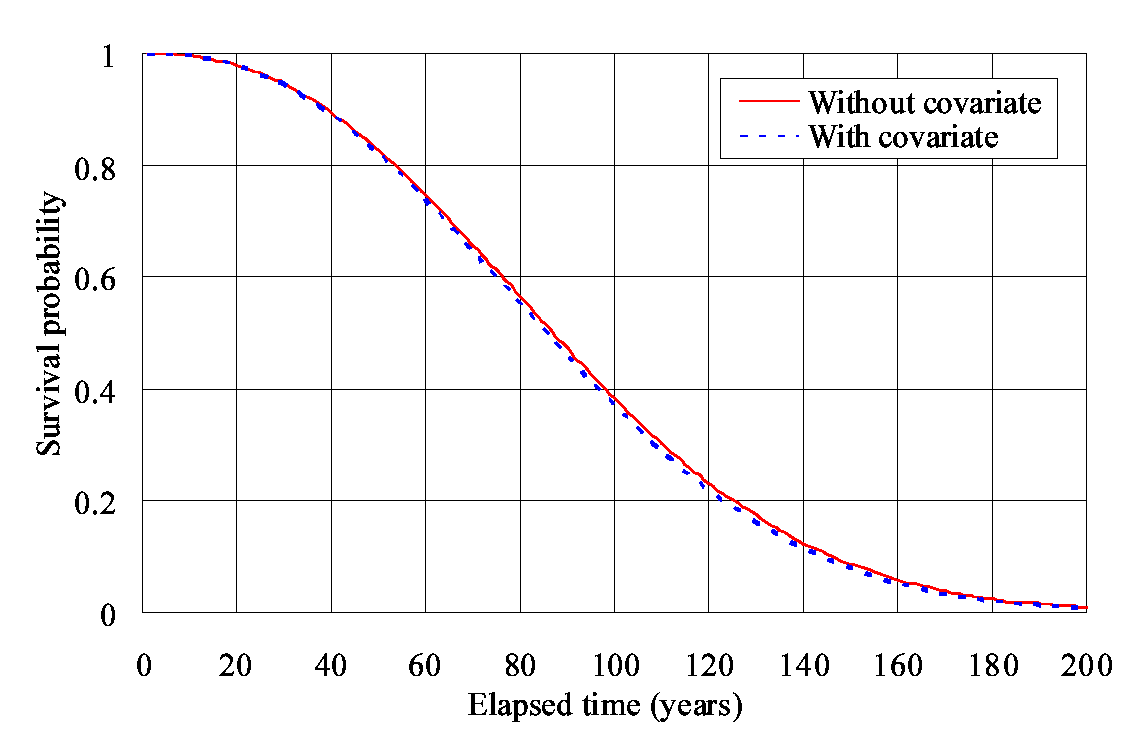
\includegraphics[scale=0.5]{fig53} 
\end{center}
\caption{Survival Probabilities of Type F With and Without Covariates.}
\label{fig53} 
\end{figure}
%
\begin{figure}[t]
\begin{center}
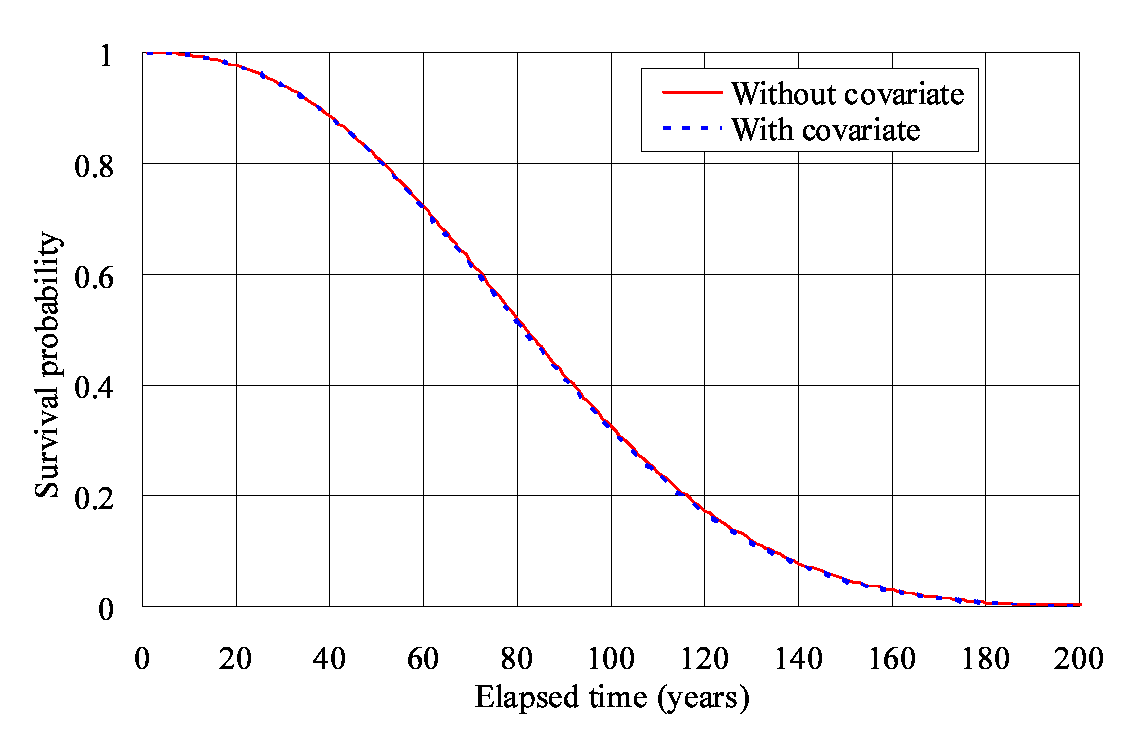
\includegraphics[scale=0.5]{fig54} 
\end{center}
\caption{Survival Probabilities of Type FL With and Without Covariates.}
\label{fig54} 
\end{figure}
%
\begin{figure}[t]
\begin{center}
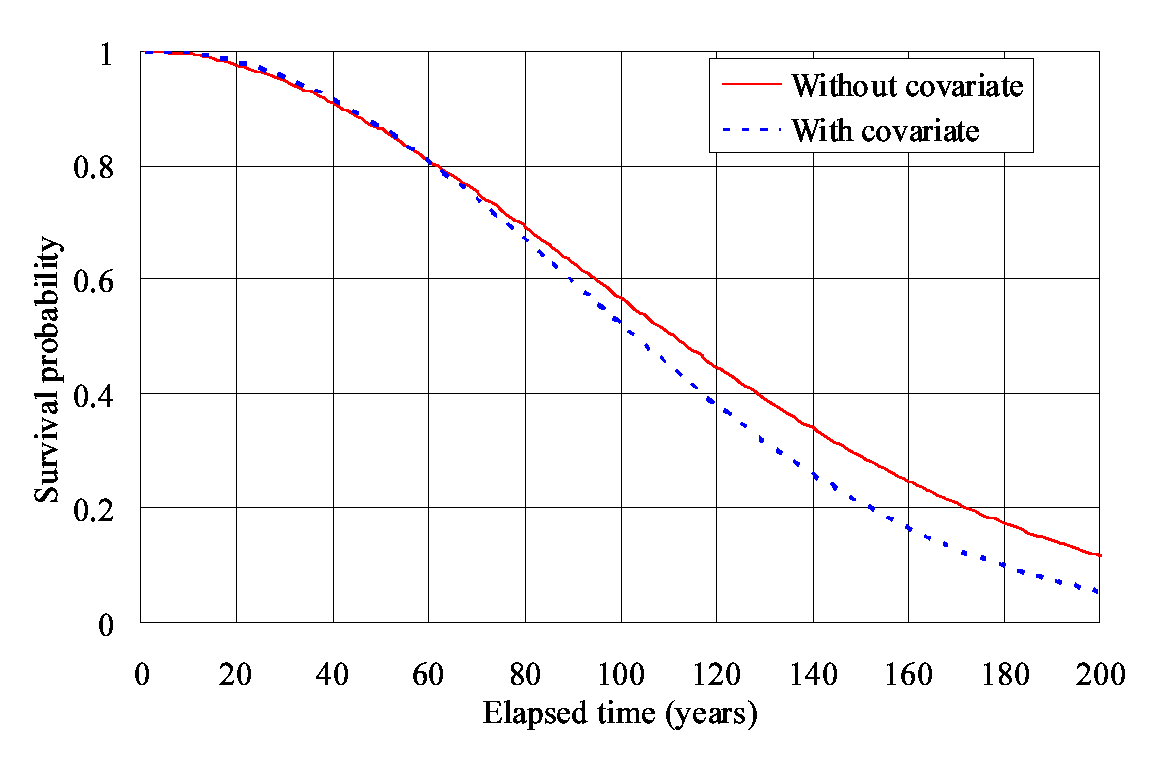
\includegraphics[scale=0.5]{fig55} 
\end{center}
\caption{Survival Probability of Type A With and Without Covariates.}
\label{fig55} 
\end{figure}
%%%%%%%%%%%
A comparative look in the survival probability curve of each pipeline type is drawn in Figure \ref{fig56}. As can be seen from the figure, pipeline type C and FL have faster decrease than pipeline type F. However, all three old pipeline types exert to has $0.5$ probability of being broken after 80 years in operation. On the other hand, pipeline type A deems to has much longer life expectancy than the others.
\begin{figure}[t]
\begin{center}
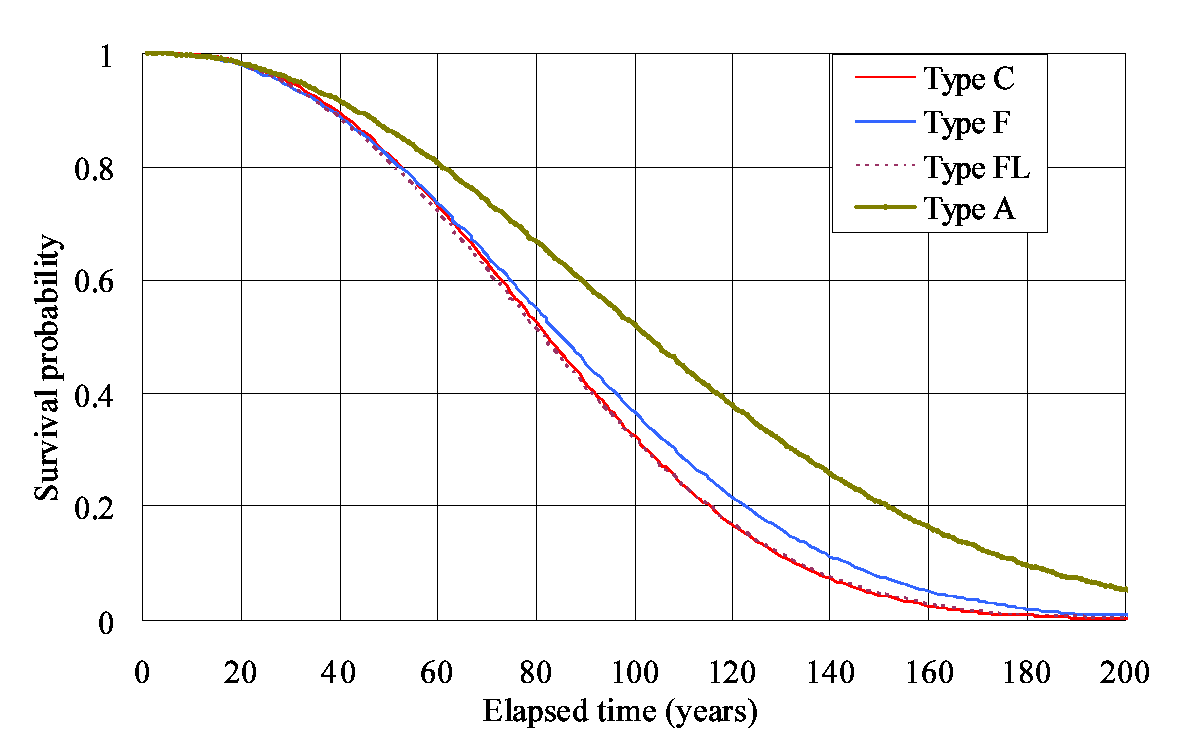
\includegraphics[scale=0.5]{fig56} 
\end{center}
\caption{Survival probabilities among Different Types of Pipelines.}
\label{fig56} 
\end{figure}
%
\subsubsection{Optimal renewal time and expected life cycle cost}
\label{5822}
Estimation for optimal renewal time and expected life cycle cost is carried out in the second phase after obtaining the values for Weibull's parameters and the associate costs. Minimization principle to seek for the optimal duration $z^*$ is empirical analyzed by using equations (\ref{han1}- \ref{sa}). Results of estimation are presented in Figure \ref{fig57} for benchmark case ($C$ = $5$ million Yen for social cost, $I=1$ million Yen for direct repair cost and $\rho=0.04$ for discount rate). It ought to recognize that the optimal renewal duration is in the range of 50 to 60 years for old types of pipelines and about 80 years of optimal renewal duration for type A.
\begin{figure}[t]
\begin{center}
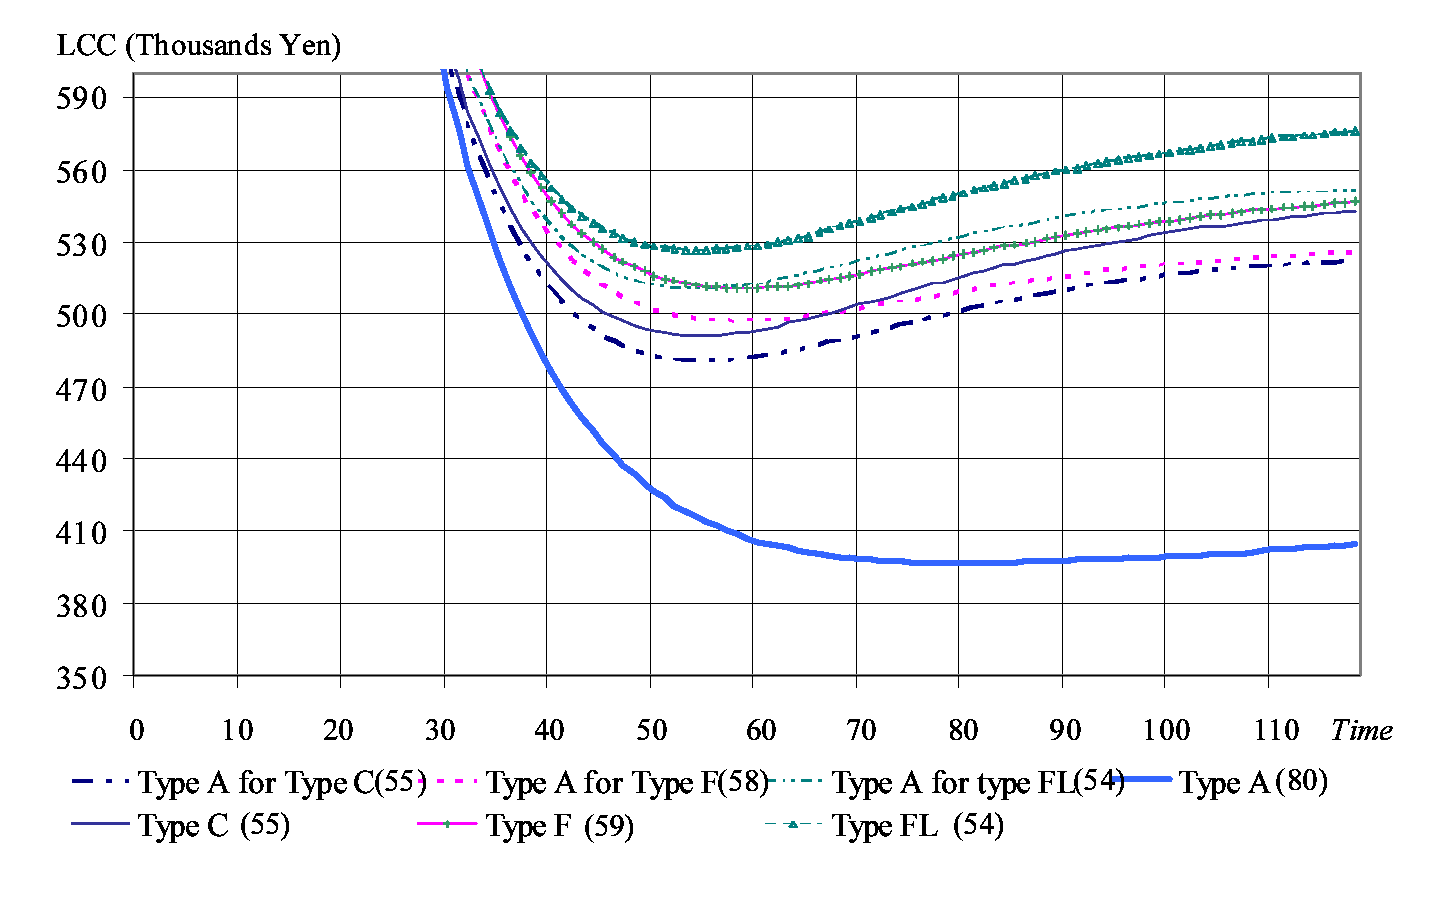
\includegraphics[scale=0.5]{fig57} 
\end{center}
\caption{Comparision of Expected Life Cycle Cost with Switching Curves.}
\label{fig57} 
\end{figure}
%%%%%%%%%%%%%%%%%%%%%%%%%%%%%%%%%%%%%%%%%%%%%%
%%%%%%%%%%%%%%%%%%%%%%%%%%%%%%%%%%%%%%%%%%%%%%
\subsubsection{Switching Rate}
\label{5823}
Figure \ref{fig57} further describes the changes of LCC for respective old types of pipelines when using type A for replacement. In this case, the optimal renewal years yield slightly shorter than if using the old types of pipeline. For example, if using type A to replace type F, the optimal renewal duration is 59 years instead of 58 years. Based on the definition in equation (\ref{han2}), the switching rate for type C, F and FL are ($\Theta_{A-C}=55/55=1.000$), ($\Theta_{A-F}=58/59=0.983$), ($\Theta_{A-FL}=54/55=0.981$) respectively.
\subsubsection{Sensitivity Analysis}
\label{5824}
It is important to note that the expected optimal renewal time and its associated cost for respective type of pipelines depend strongly on three parameters social cost $C$, direct repair cost $I$ and the discount rate $\rho$. Any change in the values of these parameters could positively lead to large variation in term of optimal renewal years and expected life cycle cost. Thus, sensitivity analysis with ranges in values of parameters should be referred so as to provide a thoughtfully observation into the selection \cite{senanalysis}. Results are shows in Figure \ref{fig58}, Figure \ref{fig59} and Figure \ref{fig510} depicting relationship between optimal renewal duration and discount factor $\rho$, social cost $C$ and direct repair cost $I$, which applies for the renewal case of pipeline type C.

\begin{figure}[t]
\begin{center}
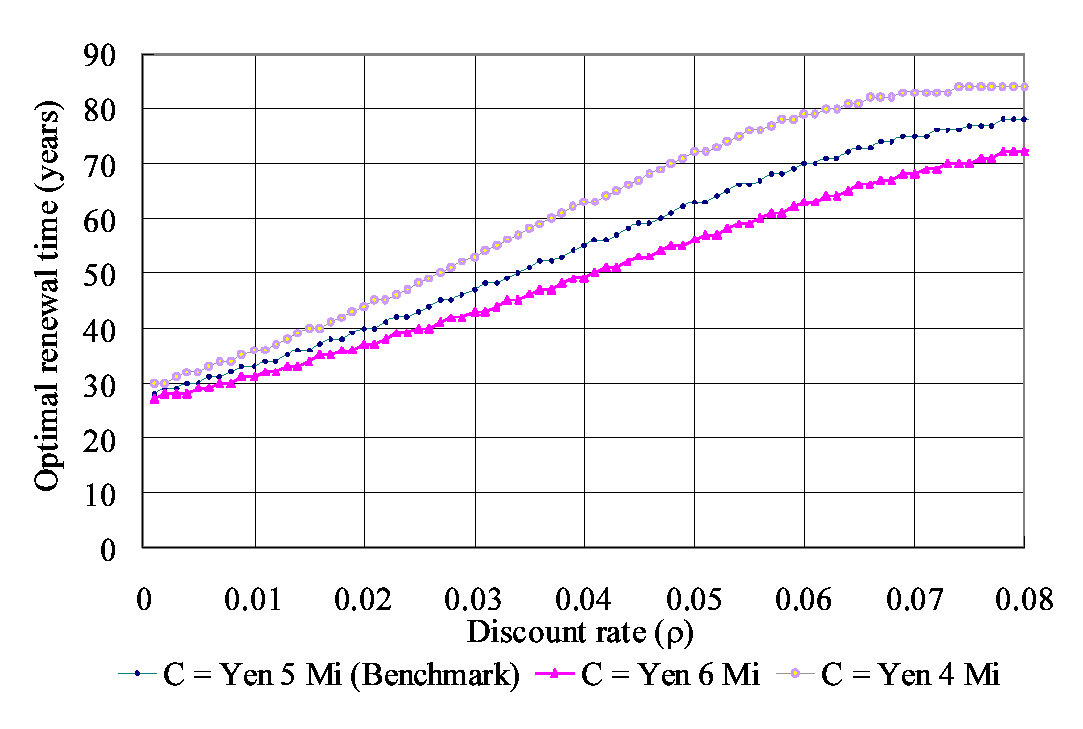
\includegraphics[scale=0.5]{fig58} 
\end{center}
\caption{Sensitivity Analysis-range of Discount Rate $\rho$.}
\label{fig58} 
\end{figure}
%
\begin{figure}[t]
\begin{center}
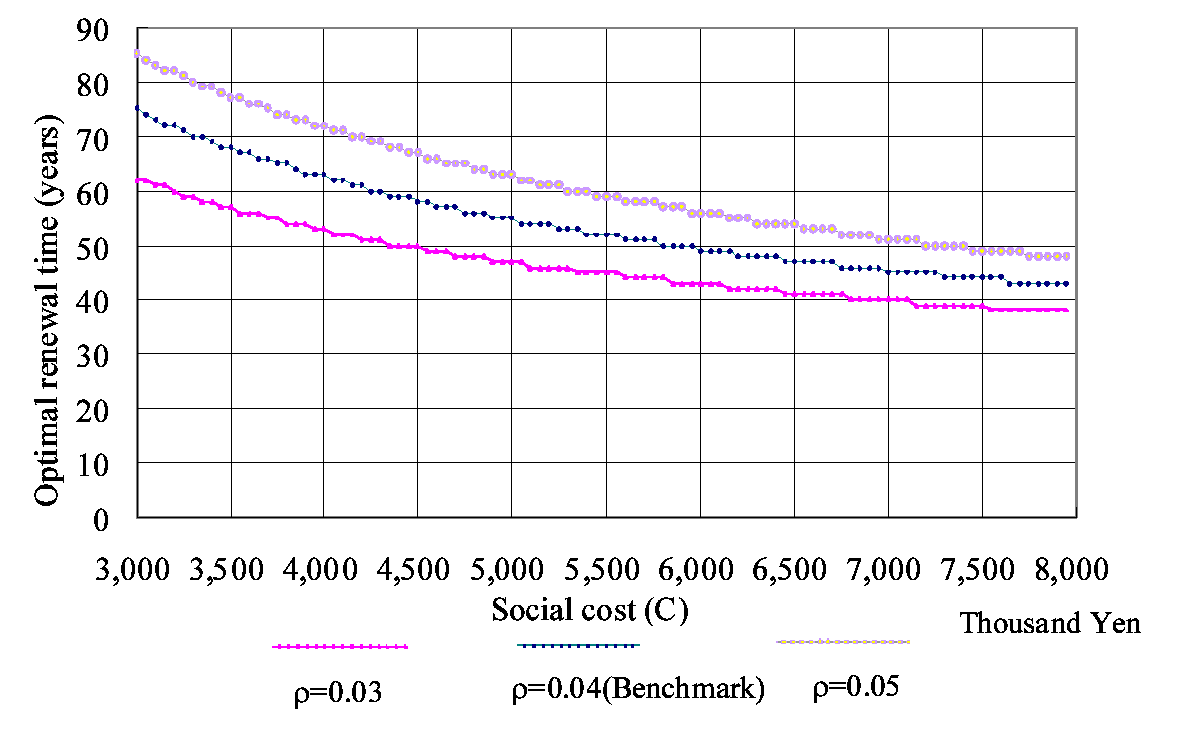
\includegraphics[scale=0.5]{fig59} 
\end{center}
\caption{Sensitivity Analysis-range of Social Cost $C$.}
\label{fig59} 
\end{figure}
%
\begin{figure}[t]
\begin{center}
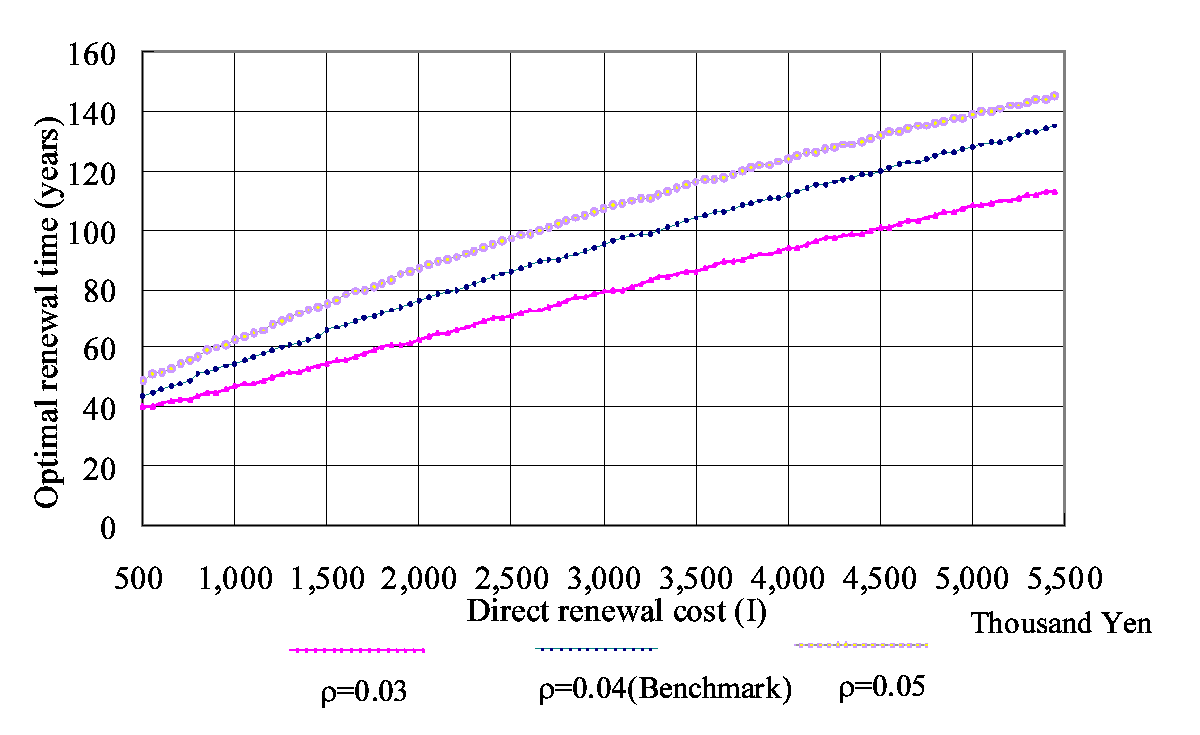
\includegraphics[scale=0.5]{fig510} 
\end{center}
\caption{Sensitivity Analysis-range of Direct Repair Cost $I$.}
\label{fig510} 
\end{figure}

Figure \ref{fig58} draws the change in optimal renewal years when changing the value of discount factor $\rho$. Benchmark optimal renewal duration curve is referred in the case of keeping $C$ = $5$ million Yen, $I$ = $1$ million Yen. Changing in value of either $C$ or $I$ consequently affects the optimal duration for renewal. For example, as can be seen from the figure, comparing to the benchmark case, increasing social cost $C$ = $1$ million relatively reduces the optimal duration about 3 to 10 years. Moreover, when $\rho$ becomes either very small (going close to $0$) nor large, convergence of optimal duration are obtained. Convergence of optimal duration is also realized when $\rho$ receives its value greater than $0.1$. High slope of optimal duration curve is acknowledged when $\rho$ $\le$ $0.05$.

The relationship between optimal renewal duration and change in social cost is sketched in Figure \ref{fig59}. It is realized that the increment in social cost results in the gradual shrink of optimal renewal duration. For example, if $500$ thousand Yen is added up to the benchmark case when keeping the same $I$ = $1$ million Yen and $\rho$ = $0.04$, the optimal duration is shortened about 6 to 10 years. 

Figure \ref{fig510} shows the correlation between optimal renewal duration and change in value of direct repair cost $I$. The linear rise of the curve proves a fact that higher direct repair cost leads to higher optimal renewal duration. For benchmark case ($C$ = $5$ million Yen, $I$ = $1$ million yen and $\rho$ = $0.04$), if happening the increase of $500$ thousand Yen in $I$, the optimal renewal duration goes up about 3 to 10 years. In the case when changing the discount factor $\rho$, it is found that the lower value of discount factor is, the smaller variation of optimal duration becomes.

In the case of using average cost analysis, the changes of optimal renewal years against social cost and direct renewal cost are plotted in Figure \ref{fig511}. In this Figure, we assume a constant value of direct cost $I=1$ million Yen when social cost change in the range from $1$ Million Yen to $20$ Million Yen. On the other hand, when direct cost $I$ changes, the social cost $C$ is assumed to equal to $5$ Million Yen. All relative costs are approximately calculated for pipelines with relative length of $140$ m. It is noted from this point that, the range of assumption value for either social cost and direct cost can be changed depending on various local conditions where analysis is deem applicable.
\begin{figure}[t]
\begin{center}
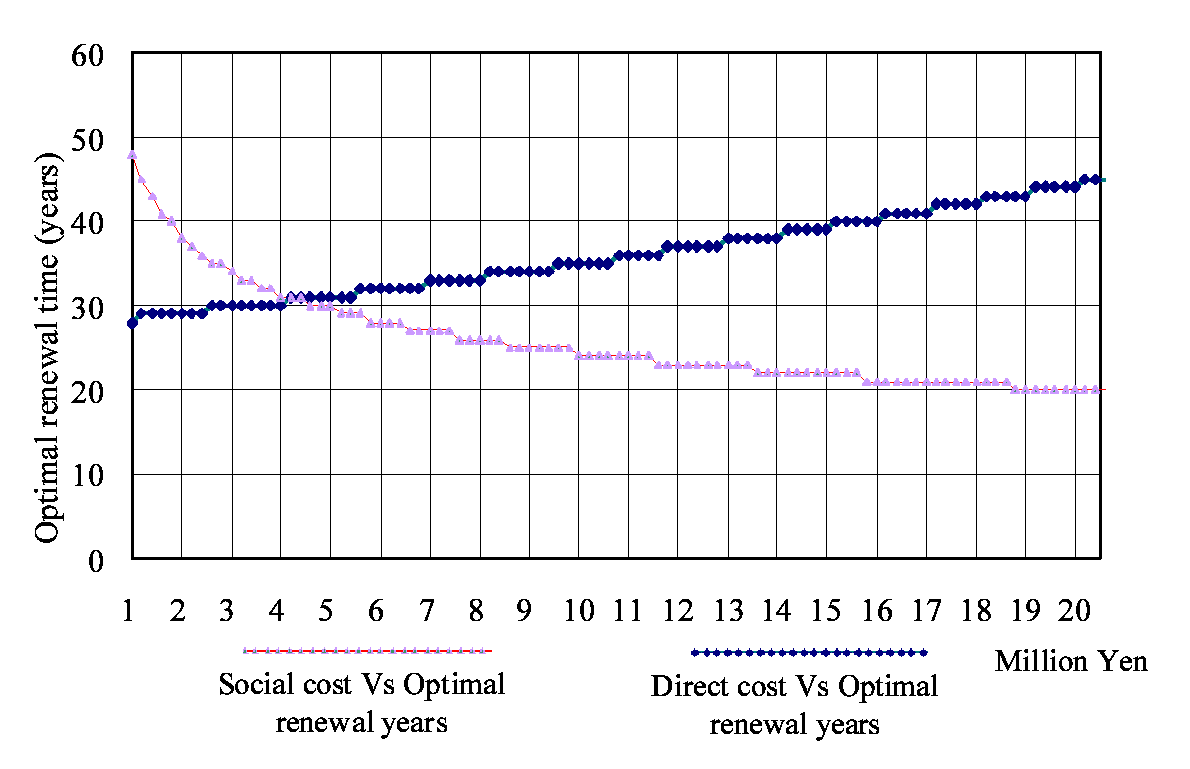
\includegraphics[scale=0.5]{fig511} 
\end{center}
\caption{Sensitivity Analysis - Average Cost.}
\label{fig511} 
\end{figure}
%%%%%%%%%%%%%%%%%%%%%%%%%%%%%%%%%%%%%%%%%%%%%%
\section{Summary and Recommendations}
\label{59}
%%%%%%%%%%%%%%%%%%%%%%%%%%%%%%%%%%%%%%%%%%%%%%
This chapter has presented a methodology to estimate the optimal renewal time of pipeline systems. The Weibull hazard function was employed to evaluate the survival probability of each types of pipeline with respect to the diameter. The mathematical formulation for calculating the total expected life cycle cost was introduced. The total expected life cycle cost took into account social cost and direct renewal cost in the event of leakage or breakdown of the pipeline. A system of water distribution network is comprised of many types of pipe materials, some of which might better be replaced to the optimal type of pipeline with pre-determined plan according to their forecasted survival probability. This is of crucial importance to uphold the safety level of the entire system, especially in the mega cities. 

An empirical application of the model to the water supply pipeline system in Osaka city was carried out. Results of the estimation identified the optimal renewal time for each type of pipeline. Sensitivity analysis reveals social cost $C$ and discount factor $I$ as important input factors of the model. These two values should be thoughtfully calculated for a more accurate outcome of optimal renewal time and concerning LCC. From the application view point, this model can be applied not only to water distribution networks but also to other types of underground infrastructure system. % Time-dependence repair strategy: Pipelines systems

% Chapter 6

\chapter{Mixture Hazard Model and Benchmarking Approach} % Write in your own chapter title
\label{Chapter6}
\lhead{Chapter 6. \emph{Mixture Hazard Model and Benchmarking Approach}} % Write in your own chapter title to set the page header
%
%%%%%%%%%%%%%%%%%%%%%%%%%%%%
\section{General introduction}
\label{61}
The statistical hazard models based on the visual inspection data have been widely practiced in the field of infrastructure asset management. In the models, Markov chain theory with it presumption of accuracy and generality to real data has been usefully applied. Furthermore, with use of Markov decision process, decision making process can gain the advantage for management of infrastructure system, especially at strategic and macroscopic level.
 
In addition to the decision making process at strategic level, it is necessary to develop a model which can be applied to generate information for various levels. For example, in bride management, a concrete maintenance plan for some important individual components is important; this plan can be regarded as for ``component level''. In fact, deterioration processes of individual components under the same structural characteristic and an environmental condition are also different. Therefore, in order to develop a more exquisite deterioration forecast technique, it is acknowledged to consider the heterogeneity of the deterioration process of individual components which are under the same structural characteristic and environmental condition. This Markov deterioration hazard model differs from the model, which also employs Markov transition probability based on the total of huge deterioration information and average deterioration process.

However, in fact, there is obvious not much comprehensive study on Markov deterioration model that pays great attention on the heterogeneity of the deterioration process. These might due to constrains like facing accuracy and efficiency of collected information, increasing work load of business and management...etc, which limited previous studies on establishing sound assumptions to heterogeneity factor. Therefore, the development of a more efficient deterioration forecast technique in consideration with the heterogeneity of the deterioration process is mandatory.

The favor for mixture model and benchmarking approach is further rendered by the quest for the selection of best pavement technology, particularly based on material, structure and construction technique. This quest is realized in high attention, especially in the developing nations \cite{kcleong}. Therefore, beside the analytical method for mixture model, this chapter extends its words on benchmarking study. 

A good example of benchmarking application is the case of Vietnam, where the entire road system is comprised of many different technologies. Reason to this is, as the matter of fact, due to limited capacity, the country often borrowed technologies from abroad. National standards for design and construction practices are somewhat mimic versions of guidelines, most of them are copied from developed nations. This practice is definitely unlike to that of developed nations. Consequently, leads to huge amount of efforts and budget in monitoring and maintenance during operation phases. Hence, in view of long term and strategic management, there is a strong demand in searching for the best pavement technology, which could become a national standard in pavement management system. 

%%%%%%%%%%%%%%%%%%%%5
\section{Heterogeneity and Sampling Population}
\label{62}
As a matter of fact, deterioration speed of one infrastructure component is always different from the other even thought they share the same structural characteristics. This is due to the fact that each component bears different working environment from the other. For instance, the cracking rate of pavement section often contains some degree of variation from each other even they belongs to a short distance road length. With respect to the deterioration speed of the infrastructure with similar characteristics, it is often the case that, only representing deterioration curve is drawn in connection to average hazard rate. Without any exception, Markov hazard model is used to estimate this average value. In a broaden understanding, suffice to say that the average value of hazard rate is actually added or weighted by individual hazard rate of each component or each group of similar component. 

Probabilistically, hazard rate of individual component is distributed around the mean of average value. An illustration of this situation is sketched in Figure \ref{fig61}. As can be seen from the figure, at time $\tau_i$ the estimated condition state from forecasting model is $i$. However, deterioration speed of individual can be either faster or slower than the average curve as showed in dotted lines.
%
\begin{figure}[t]
\begin{center}
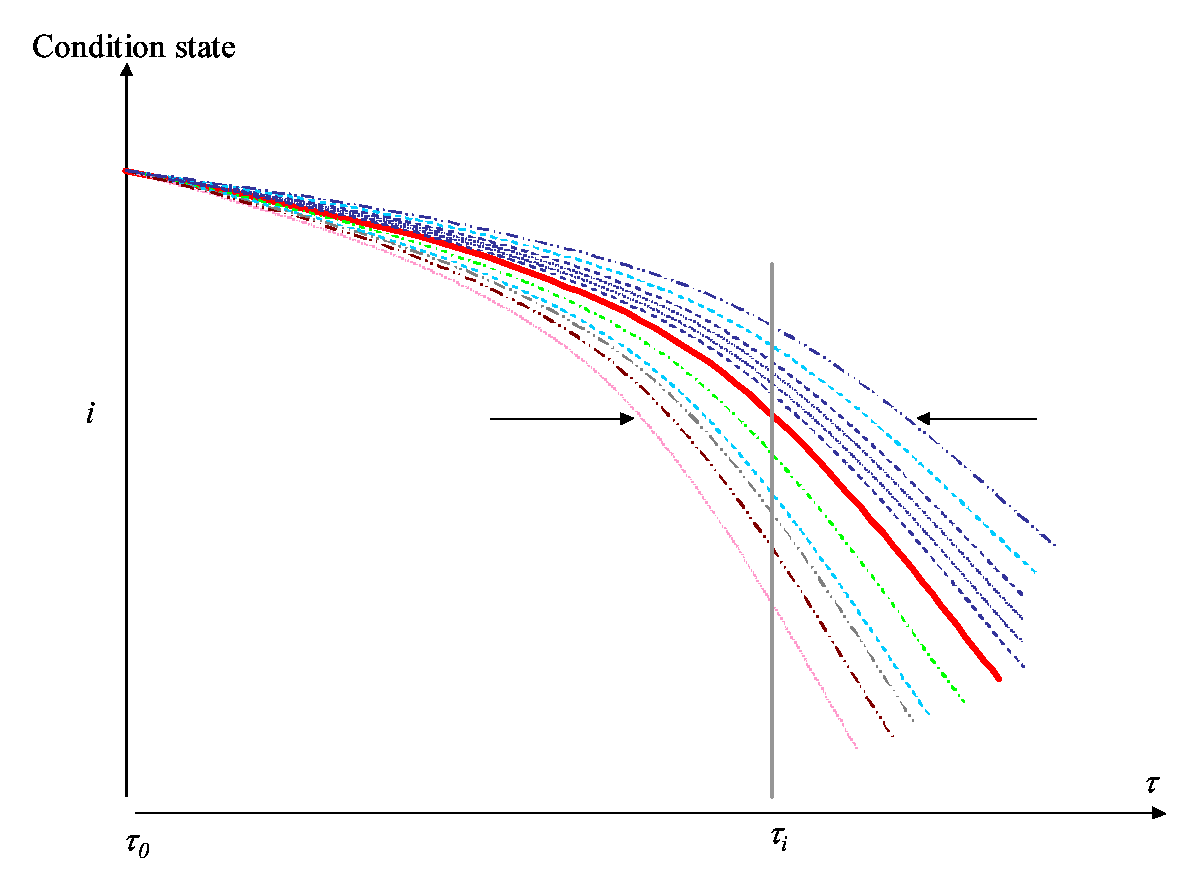
\includegraphics[scale=0.5]{fig61} 
\end{center}
\footnotesize Note) Each line represents for deterioration curve of individual road section or group of road sections with similar characteristics.
\caption{Deterioration curve differences.}
\label{fig61} 
\end{figure}
%
%%%%%%%%%%%%%%%%%5
\section{Mixture Markov deterioration hazard model}
\label{64}
\subsection{Markov transition probability and heterogeneity factor}
\label{641}
In reality, deterioration process varies differently among pavement groups due to dynamic factors. Thus, it is hard to grant a homogeneous sampling population in estimation. To express this inhomogeneous sampling population, many literatures in liability modeling employ the term ``heterogeneity factor''. In pavement system, we assume the entire road system comprising of $K$ group of road according to their technological difference. In each group $k (k=1,...,K)$, total road section is $S_k$. And $\varepsilon^k$ is referred as the heterogeneity factor, which infers the change of characteristic of a peculiar hazard rate $i(i=1,...,I-1)$ to a pavement section $s_k(s_k=1,\cdots,S_k)$. Thus, the mixture form of hazard function, which mentioned in equation (\ref{hazard}) of Chapter \ref{Chapter2}, can be defined:
\begin{eqnarray}
&& \lambda_i^{s_k} = \tilde{\lambda}_i^{s_k}\varepsilon^k \hspace{5mm}
 (i=1,\cdots,I-1;k=1,\cdots,K;s_k=1,\cdots,S_k).  \label{hu1}
\end{eqnarray}
$\varepsilon^k$ is always non-negative. In addition, it is understood that the higher value of $\varepsilon^k$ is, the faster deterioration speed of road section $s_k$ comparing to others. Within the one group of road sections (or one technology), the hazard rate of all ratings holds the same the value of the heterogeneity factor $\varepsilon^k$. Counting all the road sections as a whole, the distribution of $\varepsilon^k$ is exactly representing the influence of individual group of road sections on the overall deterioration process. Depending on structural characteristic of each system, heterogeneity factor $\varepsilon^k$ can be in form of a function or stochastic variable.

For measurable representation, we denote a set of value of $\varepsilon^k$ $(k=1,..,K)$ as a vector $\bar{\varepsilon}^k$. The bar [$\bar {\hspace{2mm}}$] indicates measurable value. As a result, we can further expressed the survival probability in equation (\ref{prop-bFla}) by means of mixed hazard rate in equation (\ref{hu1}) for pavement group $k$:
\begin{eqnarray}
&& \tilde{F}_i(y_i^{k})=\exp(-\tilde{\lambda}_i\bar{\varepsilon}^k y_i^k) .\label{prop1}
\end{eqnarray}
Siminarly, Markov transition probability expressed in equations (\ref{p1})-(\ref{pj}) are derived as follows:
\begin{manyeqns}
&& \pi_{ii}^k(z^k:\bar{\varepsilon}^k)=\exp(-\tilde{\lambda}_i^k\bar{\varepsilon}^k z^k), \label{prop2}\\
&& \pi_{ij}^k(z^k:\bar{\varepsilon}^k)=\sum_{l=i}^{j}
\prod_{m=i,\neq l}^{j-1}\frac{\tilde{\lambda}_m^k}{\tilde{\lambda}_{m}^k-\tilde{\lambda}_{l}^k} \exp (-\tilde{\lambda}^{k}_l\varepsilon^k z^k)\nonumber\\
&& \hspace{10mm} =\sum_{l=i}^{j}\psi_{ij}^l(\tilde{\mbox{\boldmath$\lambda$}}^k) \exp (-\tilde{\lambda}_{l}^k \varepsilon^k z^k) \label{poi1}\\
&& (i=1,\cdots,I-1;j=i+1,\cdots,I;k=1,\cdots,K), \nonumber
\end{manyeqns}
where
\begin{eqnarray}
&& \psi_{ij}^l(\tilde{\mbox{\boldmath$\lambda$}}^k)=
\prod_{m=i,\neq l}^{j-1}\frac{\tilde{\lambda}_m^k}{\tilde{\lambda}_{m}^{k}-\tilde{\lambda}_{l}^k}. \label{psi}
\end{eqnarray}
\subsection{Parametric approach to heterogeneity factor $\varepsilon$}
\label{642}
In parametric approach, the heterogeneity factor $\varepsilon^k$ is assumed as a probability sample extracted from Gamma distribution $f(\varepsilon^k:\alpha,\gamma)$:  
\begin{eqnarray}
&& f(\varepsilon^k:\alpha,\gamma)=\frac{1}{\gamma^\alpha \Gamma(\alpha)}\left(\varepsilon^k\right)^{\alpha-1}\exp\left(-\frac{\varepsilon^k}{\gamma}\right). \label{gamma}
\end{eqnarray}
Gamma distribution $f(\varepsilon:\alpha,\gamma)$ has its mean $\mu=\alpha.\gamma$ and standard variance $\sigma^2=\alpha.\gamma^2$. In addition, if $\alpha=1$, it turns to be exponential distribution. For handy calculation in the following writings, the mark $k$ is temporary omitted. The life expectancy of condition state $i$ keep unchanging until or more than the time $y_i$ in equation \ref{prop1} is actually the transition probability $\pi_{ii}$:
%%%%%%%%%%
\begin{eqnarray}
&& \tilde{\pi}_{ii}(z)=\int_0^\infty \pi_{ii}(z:\varepsilon)f(\varepsilon:\alpha,\gamma)d\varepsilon \nonumber \\
&& \hspace{5mm} =\int_0^\infty \exp(-\tilde{\lambda}_i\varepsilon z)
\frac{1}{\gamma^\alpha \Gamma(\alpha)}\varepsilon^{\alpha-1}\exp\left(-\frac{\varepsilon}{\gamma}\right)d\varepsilon \nonumber \\
&& \hspace{5mm}=\frac{1}{\gamma^\alpha \Gamma(\alpha)}\int_0^\infty \exp\left\{\left(-\tilde{\lambda}_i z-\frac{1}{\gamma}\right)\varepsilon\right\}\varepsilon^{\alpha-1}d\varepsilon \nonumber\\
&& \hspace{10mm}(i=1,\cdots,I-1) . \label{prp11}
\end{eqnarray}
%%%%%%%%%%%%%%%%%%%%%

By setting $u_i=(\tilde{\lambda}_i z+\frac{1}{\gamma})\varepsilon$, equation \ref{prp11} becomes
\begin{eqnarray}
&& \tilde{\pi}_{ii}(z)=\frac{1}{\gamma^\alpha \Gamma(\alpha)}\int_0^\infty \exp(-u_i)\left(\frac{u_i}{{\tilde{\lambda}_i z+\frac{1}{\gamma}}}\right)^{\alpha-1} 
 \frac{1}{{\tilde{\lambda}_i z+\frac{1}{\gamma}}} du_i \nonumber \\
&& \hspace{3mm}=\frac{1}{\gamma^\alpha \Gamma(\alpha)}\left(\frac{1}{{\tilde{\lambda}_i z+\frac{1}{\gamma}}}\right)^\alpha \int_0^\infty \exp(-u_i)u_i^{\alpha-1}  du_i \nonumber \\
&& \hspace{3mm}=\frac{1}{\gamma^\alpha \Gamma(\alpha)}\left(\frac{1}{{\tilde{\lambda}_i z+\frac{1}{\gamma}}}\right)^\alpha \Gamma(\alpha) 
=\frac{1}{(\tilde{\lambda}_i \gamma z+1)^\alpha}.
\end{eqnarray}
%%
In general case, the Markov transition probability of changing condition state from $i$ to $j$ under time interval $z$ will be
%%
\begin{eqnarray}
&& \tilde{\pi}_{ij}(z)=\int_0^\infty \pi_{ij}(z:\varepsilon)f(\varepsilon:\phi)d\varepsilon \nonumber \\
&& \hspace{5mm} = \int_0^\infty \sum_{l=i}^j \psi_{ij}^l(\tilde{\mbox{\boldmath$\lambda$}})\exp(-\tilde{\lambda}_l\bar{\varepsilon} z) f(\varepsilon:\alpha,\gamma) d\varepsilon \nonumber \\
&&  \hspace{5mm}=\sum_{l=i}^j \frac{\psi_{ij}^l(\tilde{\mbox{\boldmath$\lambda$}})}{\gamma^\alpha \Gamma(\alpha)}\int_0^\infty \exp\left\{\left(-\tilde{\lambda}_l z-\frac{1}{\gamma}\right)\varepsilon\right\}\varepsilon^{\alpha-1}d\varepsilon \nonumber \\
&& \hspace{5mm}=\sum_{l=i}^j\frac{\psi_{ij}^l(\tilde{\mbox{\boldmath$\lambda$}})}{(\tilde{\lambda}_l \gamma z+1)^\alpha}.
\end{eqnarray}
%%%
With existence of the heterogeneity factor $\varepsilon^k$, hazard rate of individual group is thought to be distributed as agreeing to average hazard rate $\tilde{\lambda}_i$. In this understanding, it is therefore assume for the Gamma distribution to have its mean of $1$ and standard variance of $1/\phi$. As a result, we can obtain the explicit form of Markov transition probability with respect to distribution of heterogeneity factor:
%%
\begin{manyeqns}
&& \tilde{\pi}_{ii}(z)=\frac{\phi^\phi}{(\tilde{\lambda}_i z+\phi)^\phi}, \label{ptpi410} \\
&& \tilde{\pi}_{ij}(z)=\sum_{l=i}^j \frac{\psi_{ij}^l(\tilde{\mbox{\boldmath$\lambda$}})\phi^{\phi}}{({\tilde{\lambda}_l z+\phi})^\phi}  ,\label{ptpi411} \\
&& (i=1,\cdots,I-1;j=i+1,\cdots,I) .\nonumber
\end{manyeqns}
%%%%%%%%
\subsection{Semi-parametric approach to heterogeneity factor $\varepsilon$}
\label{643}
A great deal of past research has revealed the difficulties in defining the heterogeneity factor $\varepsilon^k$. The assumption of the heterogeneity factor to be in the form of a function or a stochastic variable crucially depends on the characteristics of the system itself and the availability of monitoring data \cite{lancaster90,Marriott06}. This section focuses on applying mixture model in the case that the value distribution of heterogeneity factor $\varepsilon^k$ has a small dispersion. In other words, the departure of heterogeneity factor $\varepsilon^k$ from homogeneity is in a small scale. This type of mixture model is named as the local mixture model. In exponential family form $f(x;\epsilon)$ (where $x$ and $\epsilon$ are the variable and heterogeneity respectively), local mixing mechanism is defined via its mean parameterization $\delta^{k}$: 
%%%%
\begin{eqnarray}
g(x;\mu) : = f(x;\epsilon) + \sum_{i=2}^{r}f^{k}(x;\epsilon),\label{locami} 
\end{eqnarray}
where
\begin{eqnarray}
f^{k}(x;\epsilon)=\frac{\delta^{k}}{\delta\epsilon^{k}}f(x;\epsilon). \nonumber
\end{eqnarray}
%%%
Another class of the local mixture model that captures the behavior of scale dispersion in mixture value of function $f(x;\epsilon)$, is defined as the local scale mixture model.
\begin{eqnarray}
g(x;\epsilon) : = f(x;\epsilon) + \sum_{i=2}^{r}\frac{\epsilon^k}{k!}f^{k}(x;\epsilon). \label{localscal} 
\end{eqnarray}
Expansion of functions in equations (\ref{locami}) and (\ref{localscal}) can be seen to follow the Taylor series. Since the likelihood function of Markov transition probability in equations (\ref{locami}) and (\ref{localscal}) belongs to the exponential family. It is possible to approximate the transition probability as in the form of the local mixture distribution. 
%
\begin{eqnarray}
&& \tilde{\pi}_{ij}(z)=\int_0^\infty \pi_{ij}(z:\varepsilon)f(\varepsilon)d\varepsilon 
 (i=1,\cdots,I-1) . \label{prp12}
\end{eqnarray}
%
For convenience of mathematical manipulation, the local mixture transition probability is assumed as an exponential function $f_{mix}(\epsilon,z,\lambda)$ with $mix$ indicating the abbreviation of mixture. As the sequent, the mixture function $f_{mix}(\epsilon,z,\lambda)$ can be described by means of standard function $f(\epsilon,z,\lambda)$ and distribution $H(\varepsilon)$. Equation (\ref{prp12}) is further simplified as 
%%
\begin{eqnarray}
f_{mix}(\varepsilon,z,\lambda) = \int{f(\varepsilon,z,\lambda)}dH(\varepsilon), \label{prp2}
\end{eqnarray}
%
where $f(\varepsilon,z,\lambda)=exp(-\varepsilon\lambda z)$. Function $f(\varepsilon,z,\lambda)$ is likely a function of $\varepsilon$ about its mean. Without no loss of generality, and as long as the mean exist, we can further decompose equation (\ref{locami}) as follows:
\begin{eqnarray}
exp(-\varepsilon\lambda z)=e^{-\lambda z}(1+(\epsilon -1)(-\lambda z) 
+\frac{(\epsilon-1)^2}{2!}(-\lambda z)^2+ ... \hspace{2mm}.\label{taylor1}
\end{eqnarray}
This is the Taylor series. And thus, the quadratic form (when r = 2) is acceptable for an accurate approximation. Consequently, an explicit form of approximation can be derived for the Markov transition probability:
%
\begin{eqnarray}
E(e^{-\varepsilon\lambda z}) \approx e^{-\lambda z}\lbrace 1 + \frac{(\sigma\lambda z)^{2}}{2}\rbrace  \label{locfinal}
\end{eqnarray}
and
\begin{manyeqns}
&& \tilde{\pi}_{ii}(z) = e^{-\tilde{\lambda}_iz}\lbrace 1  + \frac{(\sigma\tilde{\lambda}_iz)^2}{2!}\rbrace, \label{piii} \\
&& \tilde{\pi}_{ij}(z) = \sum_{l = i}^j \psi_{ij}^l(\tilde{\mbox{\boldmath$\lambda$}})e^{-\tilde{\lambda}_lz}\lbrace 1 + \frac{(\sigma\tilde{\lambda}_lz)^2}{2!}\rbrace ,\label{piij}\\
&&(i=1,\cdots,I-1; j=i+1,\cdots,I). \nonumber
\end{manyeqns}

%%%%%%%%%%%%%%%%%%%%%%%%%%%%%%%%%%%%%%%%%%%%%%%%%%%%%%%%%%
\subsection{Likelihood estimation approach}
\label{644}
\subsubsection{Parametric estimation approach}
\label{6441}
\textit{a) Estimation assumtion}\\
%%%
The estimation of Markov transition probability and heterogeneity factor requires monitoring data from at least two visual inspections. Supposing that the periodical monitoring data of $S_k$ road sections is available. An inspection sample $s_k$ (a road section) implies two consecutive discrete periodical inspections at times $\bar{\tau}_A^{s_k}$ and $\bar{\tau}_B^{s_k}=\bar{\tau}_A^{s_k}+\bar{z}^{s_k}$, with its respective condition states $h(\bar{\tau}_A^{s_k})=i$ and $h(\bar{\tau}_B^{s_k})=j$. Based on monitoring data of $\sum_{k=1} ^K S_k$ samples, dummy variable $\bar{\delta}_{ij}^{s_k} ~ (i=1,\cdots,I-1,j=i,\cdots,I;s_k=1,\cdots,S_K;k=1,\cdots,K) $ is defined to satisfy the following conditions: 
%
 \begin{eqnarray}
      && \bar{\delta}_{ij}^{s_k}=\left\{
      \begin{array}{ll}
         1 &  h(\bar{\tau}_A^{s_k})=i,h(\bar{\tau}_B^{s_k})=j\\
         0 & Otherwise 
      \end{array}.
      \right.
   \end{eqnarray}
%
The range of dummy variable $(\bar{\delta}_{11}^{s_k},\cdots,\bar{\delta}_{I-1,I}^{s_k})$ is denoted by using the dummy variable vector $\bar{\mbox{\boldmath$\delta$}}^{s_k}$. Furthermore, structural characteristics and environment conditions of the road are expressed by means of characteristic variable vector $\bar{\mbox{\boldmath$x$}}^{s_k}=(\bar{x}_1^{s_k},\cdots,\bar{x}_M^{s_k})$, with $\bar{x}_m^{s_k}~(m=1,\cdots,M)$ indicating the observed value of variable $m$ for sample ${s_k}$. The first variable is referred as a constant term, with its value $x_1^{s_k}=1$. Thus, the information concerning monitoring data of sample $k$ can be described as $\mbox{\boldmath$\Xi$}^{s_k}=(\bar{\mbox{\boldmath$\delta$}}^{s_k},\bar{z}^{s_k},\bar{\mbox{\boldmath$x$}}^{s_k})$.

The hazard rate of condition state $i$ of sample $s_k$ can be expressed by using mixture hazard function $\lambda_i^{s_k}(y_i^{s_k})=\tilde{\lambda}_i^{s_k}\varepsilon^k ~(i=1,\cdots,I-1)$, with $I$ as the absorbing condition state satisfying the conditions $\pi_{II}^{s_k}=1$ and $\tilde{\lambda}_I^{s_k}=0$. The hazard rate $\tilde{\lambda}_i^{s_k}~(i=1,\cdots,I-1;{s_k}=1,\cdots,L_k)$ depends on the characteristic vector of the road section, and is described as follows: 
%
\begin{eqnarray}
      && \tilde{\lambda}_i^{s_k}=\mbox{\boldmath$x$}^{s_k}\mbox{\boldmath$\beta$}_i^\prime,
      \label{hazard14}
\end{eqnarray}

where $\mbox{\boldmath$\beta$} _ i=(\beta_{i,1},\cdots,\beta_{i,M}) $ is a row vector of unknown parameters $\beta_{i,m} ~ (m=1,\cdots,M) $, and the symbol ${}^\prime$ indicates the vector is transposed. From equations (\ref{piii}) and (\ref{piij}), the standard hazard rate of respective condition states can be expressed by means of hazard rate $\tilde{\lambda}_i^{s_k}~(i=1,\cdots,I-1;s_k=1,\cdots,L_k)$ and heterogeneity parameter  $\varepsilon^k$. The average Markov transition probability can be expressed in equation  (\ref{piij}), with consideration of characteristic variable $\bar{x}^{s_k} $. In addition, the transition probability depends on inspection interval $\bar{z}^{s_k}$. As a result, transition probability $\pi_{ij}$ can be expressed as a function of measurable monitoring data $(\bar{z}^{s_k},\bar{\mbox{\boldmath$x$}}^{s_k})$ and unknown parameter $\mbox{\boldmath$\theta$}=(\mbox{\boldmath$\beta$}_1,\cdots,\mbox{\boldmath$\beta$}_{I-1},\phi)$ as $\tilde{\pi}_{ij}^{s_k}(\bar{z}^{s_k},\bar{\mbox{\boldmath$x$}}^{s_k}:\mbox{\boldmath$\theta$})$. If the deterioration of road sections $l_k$ in the entire $L_K$ samples are assumed to be mutually independent, the likelihood function expressing the simultaneous probability density of the deterioration transition pattern for all inspection samples is defined \cite{tobin,amemi}:
%
 \begin{eqnarray}
      && \hspace{-3mm} {\cal L}(\mbox{\boldmath$\theta$},\mbox{\boldmath$\Xi$}) =
      \prod_{i=1}^{I-1} \prod_{j=i}^I \prod_{k=1}^{K} \prod_{s_k=1}^{S_k} 
      \left\{\tilde{\pi}_{ij}^{s_k}(\bar{z}^{s_k},\bar{\mbox{\boldmath$x$}}^{s_k}:
      \mbox{\boldmath$\theta$})\right\}^{\bar{\delta}_{ij}^{s_k}}.
      \label{logbF4}
   \end{eqnarray}
 %
By means of heterogeneity factor expressed by Gamma distribution, we further express the explicit form of the Markov transition probability in equations (\ref{ptpi410}) and (\ref{ptpi411}). 
%
\begin{manyeqns}
&& \tilde{\pi}_{ii}^{s_k}(\bar{z}^{s_k},\bar{\mbox{\boldmath$x$}}^{s_k}:\mbox{\boldmath$\theta$}) = \frac{\phi^\phi}{(\bar{\mbox{\boldmath$x$}}^{s_k}\mbox{\boldmath$\beta$}_i^\prime \bar{z}^{s_k}+\phi)^\phi} ,\label{lave1}  \\
&& \tilde{\pi}_{ij}^{s_k}(\bar{z}^{s_k},\bar{\mbox{\boldmath$x$}}^{s_k}:\mbox{\boldmath$\theta$}) = \sum_{s=i}^j \frac{\psi_{ij}^s(\mbox{\boldmath$\beta$})\phi^{\phi}}{(\bar{\mbox{\boldmath$x$}}^{s_k}\mbox{\boldmath$\beta$}_s^\prime \bar{z}^{s_k}+\phi)^\phi}, \label{lave2}\\
&& (i=1,\cdots,I-1;j=i,\cdots,I;l_k=1,\cdots,L_k;k=1,\cdots,K) .\nonumber
\end{manyeqns}

where $\psi_{ij}^s(\tilde{\mbox{\boldmath$\lambda$}}^{l_k})$ is referred to equation (\ref{psi}). Since $\bar{\delta}_{ij}^{s_k}$,$\bar{z}^{s_k}$,$\bar{\mbox{\boldmath$x$}}^{s_k}$ are known from inspection, the likelihood function (\ref{logbF4}) are functions of $\theta(\mbox{\boldmath$\beta$},\mbox{\boldmath$\phi$})$. Thus, we can apply maximum likelihood approach to estimate values of $\hat{\mbox{\boldmath$\theta$}}=(\hat{\mbox{\boldmath$\beta$}},\hat{\phi})$. For computational convenience, we further express likelihood function by means of logarithm:
%%%%%%%%%
\begin{eqnarray}
      && \hspace{-3mm} \ln {\cal L}(\mbox{\boldmath$\theta$},\mbox{\boldmath$\Xi$}) =
      \sum_{i=1}^{I-1} \sum_{j=1}^I \sum_{k=1}^K \sum_{s_k=1}^{S_k}
      \bar{\delta}_{ij}^{s_k} \tilde{\pi}_{ij}^{s_k}(\bar{z}^{s_k},\bar{\mbox{\boldmath$x$}}^{s_k}:
      \mbox{\boldmath$\theta$}).\label{lsogbF44}
   \end{eqnarray}
%%%%%%%
The estimation of $\mbox{\boldmath$\theta$}$ can be obtained by solving the optimality condition:
%%%%
\begin{eqnarray}
 \frac{ \partial \ln {\cal L}( \mbox{\boldmath$\theta$},\mbox{\boldmath$\Xi$}) }{\partial \theta_{i}}=0, \hspace{5mm} (i=1,\cdots,(I-1)M+1). \label{saitekin}
\end{eqnarray}
%%%%%
The optimal value of $\hat{\mbox{\boldmath$\theta$}}=(\hat{\theta}_1,\cdots,\hat{\theta}_{(I-1)M+1})$ are then estimated by applying a numerical iterative procedure such as Newton Method for the $(I-1)M+1$ order nonlinear simultaneous equations \cite{isoda}. Furthermore, estimator for the asymptotical covariance matrix $\hat{\mbox{\boldmath$\Sigma$}} (\hat{\mbox{\boldmath$\theta$}}) $ of the parameters is given by
%%%%
\begin{eqnarray}
&& \hat{\mbox{\boldmath$\Sigma$}}( \hat{\mbox{\boldmath$\theta$}})
= \left[ \frac{ \partial^2\ln {\cal L}( \hat{\mbox{\boldmath$\theta$}},\mbox{\boldmath$\Xi$})}{\partial \mbox{\boldmath$\theta$} \partial \mbox{\boldmath$\theta$}'}\right]^{-1}.
\end{eqnarray}
%%%%%%
The ($(I-1)M+1)\times((I-1)M+1)$ order inverse matrix of the right-hand side of the formula, composed by the elements $\partial^2\ln{\cal L}(\mbox{\boldmath$\theta$},\mbox{\boldmath$\Xi$})/\partial \theta_{i} \partial \theta_{j}$ results to be the inverse matrix of the Fisher information matrix.\\
%%%%%%%%%%%%%%%%%%%%%%%%
%%%%%%%%%%%%%%%%%%%%%%%%%%%%%%%%
%%%%%%%%%%%%
\textit{b) Heterogeneity estimation}\\
%%%%%%%%%%%%%%%
%%%%%%%%%%%%%%%%%%%
Information concerning inspection sample $s_k$ of pavement group $k$ is denoted as $\mbox{\boldmath$\xi$}^{s_{k}}~(s_{k}=1,\cdots,S^k)$. To describe the condition states of individual sample, the first and second condition states of sample $s_k$ are assumed as $i(s_k)$ and $j(s_k)$. From subsection \ref{44}, it is supposed that the parameter set $\hat{\mbox{\boldmath$\theta$}}=(\hat{\mbox{\boldmath$\beta$}}_1,\cdots,\hat{\mbox{\boldmath$\beta$}}_{I-1},\hat{\phi})$ is available. If we consider the distribution of heterogeneity factor $\varepsilon^k$ expressed by function $\bar{f} (\varepsilon:\hat{\phi})$, the probability density accounting for the transition pattern of each inspection sample $\mbox{\boldmath$\xi$}^{s_{k}}$ can be defined:
%
\begin{eqnarray}
      && \rho^{s_k}(\varepsilon^k:\hat{\mbox{\boldmath$\theta$}},\mbox{\boldmath$\xi$}^k) = \big\{\pi_{i(s_{k})j(s_{k})}^{s_k}(\bar{z}^{s_k},\bar{\mbox{\boldmath$x$}}^{s_{k}}:
\hat{\mbox{\boldmath$\beta$}},\varepsilon^k)\big\}^{\bar{\delta}_{i(s_{k})j(s_{k})}^{s_{k}}} \bar{f}(\varepsilon^k,\hat{\phi}) ,
\end{eqnarray}
where function $\bar{f}(\varepsilon^k,\hat{\phi})$ follows Gamma function as previously described. Further consideration for the entire sampling population in pavement group $k$, it is able to expressed the simultaneous occurrence probability density function concerning heterogeneity factor $\varepsilon^k$ as
%%%
\begin{eqnarray}
      && \rho^k(\varepsilon^k:\hat{\mbox{\boldmath$\theta$}},\mbox{\boldmath$\xi$}^k) = \prod_{s_{k}=1}^{S^k}\rho^{s_k}(\varepsilon^k:\hat{\mbox{\boldmath$\theta$}},\mbox{\boldmath$\xi$}^k)  
 \propto \prod_{s_{k}=1}^{S^k} \Big\{ \sum_{l=i(s_{k})}^{j(s_{k})}\psi_{i(s_{k})j(s_{k})}^l(\tilde{\mbox{\boldmath$\lambda$}}^{s_{k}}(\hat{\mbox{\boldmath$\theta$}}))\nonumber\\
&& \hspace{5mm} \exp (-\tilde{\lambda}_{l}^{s_{k}}(\hat{\mbox{\boldmath$\theta$}})\varepsilon^k \bar{z}^{s_{k}}) \Big\}^{\bar{\delta}_{i(s_{k})j(s_{k})}^{s_{k}}} 
\left\{(\varepsilon^k)^{\hat{\phi}-1}\exp(-\hat{\phi} \varepsilon^k)\right\}^{S_k}. \label{lsn} 
\end {eqnarray}
%%
The standard or average hazard rate is expressible by means of vector $\tilde{\mbox{\boldmath$\lambda$}}^{s_{k}}(\hat{\mbox{\boldmath$\theta$}}) = (\tilde{\lambda}_1^{s_{k}} (\hat{\mbox{\boldmath$\theta$}})$, $\cdots$ ,$ \tilde{\lambda}_{I-1}^{s_{k}} (\hat{\mbox{\boldmath$\theta$}}))$. Thus, average hazard rate $\tilde{\lambda}_i^{s_{k}} $ is understood to depend on the parameter $\hat{\mbox{\boldmath$\theta$}}$. To get the explicit form for computation, we further expressed equation (\ref{lsn}) in partial logarithm:
%%%
\begin{eqnarray}
&& \ln \rho^k(\varepsilon^k:\hat{\mbox{\boldmath$\theta$}},\mbox{\boldmath$\xi$}^k) 
 \propto \sum_{s_{k}=1}^{S^k} \bar{\delta}_{i(s_{k})j(s_{k})}^{s_{k}} \ln \Big\{ \sum_{m=i(s_{k})}^{j(s_{k})}\psi_{i(s_{k})j(s_{k})}^l(\tilde{\mbox{\boldmath$\lambda$}}^{s_{k}}(\hat{\mbox{\boldmath$\theta$}}))\nonumber\\
&& \hspace{2mm} \exp (-\tilde{\lambda}_{l}^{s_{k}}(\hat{\mbox{\boldmath$\theta$}})\varepsilon^k \bar{z}^{s_{k}}) \Big\} +S_k\Big\{(\hat{\phi}-1) \ln \varepsilon^k -\hat{\phi} \varepsilon^k\Big\} . \label{slss}
\end {eqnarray}
%%%%%
Optimal solution to get the value of heterogeneity factor $\varepsilon^k~(k=1,\cdots,K)$ can be evaluated through maximizing equation (\ref{slss}) with respect to $\varepsilon^k$ as variable and $\hat{\mbox{\boldmath$\theta$}}=(\hat{\mbox{\boldmath$\beta$}}_1,\cdots,\hat{\mbox{\boldmath$\beta$}}_{I-1},\hat{\sigma})$ earlier obtained:
%
\begin{eqnarray}
&& \max_{\varepsilon^k} \big\{\ln \rho^k(\varepsilon^k:\hat{\mbox{\boldmath$\theta$}},\mbox{\boldmath$\xi$}^k)\big\}. \label{sei}
\end{eqnarray}
%%%%%%%%%%%%%
%%%%%%%%%%%%%
%%%%%%%%%%%%%%%%%
\subsubsection{Semi-parametric approach}\label{6442}
In this part, the same content of writing like in the section \ref{6441} is referred. Changes are made only to the mathematical notation corresponding to local mixture model. Substantial change is difference in the properties of unknown pramater $\mbox{\boldmath$\theta$}=(\mbox{\boldmath$\beta$}_1$, $\cdots$,$\mbox{\boldmath$\beta$}_{I-1},\sigma)$ for local mixture model following Taylor series instead of $\mbox{\boldmath$\theta$}=(\mbox{\boldmath$\beta$}_1$, $\cdots$, $\mbox{\boldmath$\beta$}_{I-1},\phi)$ as for mixture hazard model with Gamma distribution\\
\label{4442}
\textit{a) Estimation assumtion}\\
By means of local mixture distribution with Taylor series, we further express the explicit form of Markov transition probability:
%%%
\begin{manyeqns}
&& \tilde{\pi}_{ii}^{s_k}(\bar{z}^{s_k},\bar{\mbox{\boldmath$x$}}^{s_k}:\mbox{\boldmath$\theta$})=e^{-\bar{\mbox{\boldmath$x$}}^{s_k}\mbox{\boldmath$\beta$}_i^\prime \bar{z}^{s_k}} \lbrace 1 + \frac{(\sigma\bar{\mbox{\boldmath$x$}}^{s_k}\mbox{\boldmath$\beta$}_i^\prime \bar{z}^{s_k})^2}{2!} \rbrace ,\label{pt28} \\
%%%%
&& \tilde{\pi}_{ij}^{s_k}(\bar{z}^{s_k},\bar{\mbox{\boldmath$x$}}^{s_k}:\mbox{\boldmath$\theta$})=\sum_{l=i}^j \psi_{ij}^l(\tilde{\mbox{\boldmath$\lambda$}})e^{-\bar{\mbox{\boldmath$x$}}^{s_k}\mbox{\boldmath$\beta$}_l^\prime \bar{z}^{s_k}}  \lbrace 1 + \frac{(\sigma\bar{\mbox{\boldmath$x$}}^{s_k}\mbox{\boldmath$\beta$}_l^\prime \bar{z}^{s_k})^2}{2!} \rbrace, \label{pt30} \\
&& (i=1,\cdots,I-1;j=i+1,\cdots,I), \nonumber
\end{manyeqns}
%%%%
where $\psi_{ij}^s(\tilde{\mbox{\boldmath$\lambda$}}^{l_k})$ is referred to equation (\ref{psi}). Since $\bar{\delta}_{ij}^{s_k}$,$\bar{z}^{s_k}$,$\bar{\mbox{\boldmath$x$}}^{s_k}$ are known from inspection, the likelihood function (\ref{logbF4}) are functions of $\theta(\mbox{\boldmath$\beta$},\mbox{\boldmath$\sigma$})$. Thus, we can apply maximum likelihood approach to estimate values of $\hat{\mbox{\boldmath$\theta$}}=(\hat{\mbox{\boldmath$\beta$}},\hat{\sigma})$. For computational convenience, we further express likelihood function by means of logarithm:
%%%%%%%%%
\begin{eqnarray}
      && \hspace{-3mm} \ln {\cal L}(\mbox{\boldmath$\theta$},\mbox{\boldmath$\Xi$}) =
      \sum_{i=1}^{I-1} \sum_{j=1}^I \sum_{k=1}^K \sum_{s_k=1}^{S_k}
      \bar{\delta}_{ij}^{s_k} \tilde{\pi}_{ij}^{s_k}(\bar{z}^{s_k},\bar{\mbox{\boldmath$x$}}^{s_k}:
      \mbox{\boldmath$\theta$}).\label{lsogbF42}
   \end{eqnarray}
%%%%%%%
The estimation of $\mbox{\boldmath$\theta$}$ can be obtained by solving the optimality condition:
%%%%
\begin{eqnarray}
&& \frac{ \partial \ln {\cal L}( \mbox{\boldmath$\theta$},\mbox{\boldmath$\Xi$}) }{\partial \theta_{i}}=0, \hspace{4mm}
 (i=1,\cdots,(I-1)M+1). \label{saiteki42}
\end{eqnarray}
%%%%%
The optimal value of $\hat{\mbox{\boldmath$\theta$}}=(\hat{\theta}_1,\cdots,\hat{\theta}_{(I-1)M+1})$ are then estimated by applying a numerical iterative procedure such as Newton Method for the $(I-1)M+1$ order nonlinear simultaneous equations \cite{isoda}. Furthermore, estimator for the asymptotical covariance matrix $\hat{\mbox{\boldmath$\Sigma$}} (\hat{\mbox{\boldmath$\theta$}}) $ of the parameters is given by
%%%%
\begin{eqnarray}
&& \hat{\mbox{\boldmath$\Sigma$}}( \hat{\mbox{\boldmath$\theta$}})
= \left[ \frac{ \partial^2\ln {\cal L}( \hat{\mbox{\boldmath$\theta$}},\mbox{\boldmath$\Xi$})}{\partial \mbox{\boldmath$\theta$} \partial \mbox{\boldmath$\theta$}'}\right]^{-1}.
\end{eqnarray}
%%%%%%
The ($(I-1)M+1)\times((I-1)M+1)$ order inverse matrix of the right-hand side of the formula, composed by the elements $\partial^2\ln{\cal L}(\mbox{\boldmath$\theta$},\mbox{\boldmath$\Xi$})/\partial \theta_{i} \partial \theta_{j}$ results to be the inverse matrix of the Fisher information matrix.\\
%%%%%%%%%%%%
%%%%
\textit{b) Heterogeneity estimation}\\
%%%%%%%%%%%%
%%%%%%%%%%%%%%%%
Information concerning inspection sample $s_k$ of the road group $k$ is denoted as $\mbox{\boldmath$\xi$}^{s_{k}}~(s_{k}=1,\cdots,S^k)$. To describe the condition states of individual sample, the first and second condition states of sample $s_k$ are assumed as $i(s_k)$ and $j(s_k)$. From subsection \ref{44}, it is supposed that the value of parameter $\hat{\mbox{\boldmath$\theta$}}=(\hat{\mbox{\boldmath$\beta$}}_1,\cdots,\hat{\mbox{\boldmath$\beta$}}_{I-1},\hat{\sigma})$ is available. If we consider the distribution of heterogeneity factor $\varepsilon^k$ in function $\bar{f} (\varepsilon:\hat{\delta})$, the probability density function, which infers the transition pattern of sample $\mbox{\boldmath$\xi$}^{s_{k}}$, can be defined as
%
\begin{eqnarray}
      && \rho^{s_k}(\varepsilon^k:\hat{\mbox{\boldmath$\theta$}},\mbox{\boldmath$\xi$}^k) = \big\{\pi_{i(s_{k})j(s_{k})}^{s_k}(\bar{z}^{s_k},\bar{\mbox{\boldmath$x$}}^{s_{k}}:
\hat{\mbox{\boldmath$\beta$}},\varepsilon^k)\big\}^{\bar{\delta}_{i(s_{k})j(s_{k})}^{s_{k}}} \bar{f}(\varepsilon^k,\hat{\sigma}) ,
\end{eqnarray}
where function $\bar{f}(\varepsilon^k,\hat{\sigma})$ follows local mixing mechanism as previously described. As for the total number of samples in group $k$, the probability density function concerning the simultaneous occurrence of transition can be further defined as
%%%
\begin{eqnarray}
      && \rho^k(\varepsilon^k:\hat{\mbox{\boldmath$\theta$}},\mbox{\boldmath$\xi$}^k) = \prod_{s_{k}=1}^{S^k}\rho^{s_k}(\varepsilon^k:\hat{\mbox{\boldmath$\theta$}},\mbox{\boldmath$\xi$}^k)  
 \propto \prod_{s_{k}=1}^{S^k} \Big\{ \sum_{l=i(s_{k})}^{j(s_{k})}\psi_{i(s_{k})j(s_{k})}^l(\tilde{\mbox{\boldmath$\lambda$}}^{s_{k}}(\hat{\mbox{\boldmath$\theta$}}))\nonumber\\
&& \hspace{5mm} \exp (-\tilde{\lambda}_{l}^{s_{k}}(\hat{\mbox{\boldmath$\theta$}})\varepsilon^k \bar{z}^{s_{k}}) \Big\}^{\bar{\delta}_{i(s_{k})j(s_{k})}^{s_{k}}} 
\left\{1 + \frac{(\sigma\tilde{\lambda}_l^{s_k}z^{s_k})^2}{2!}\right\}^{S_k} .\label{ls} 
\end {eqnarray}
%%
The standard or average hazard rate is expressible by means of vector $\tilde{\mbox{\boldmath$\lambda$}}^{s_{k}}(\hat{\mbox{\boldmath$\theta$}})=(\tilde{\lambda}_1^{s_{k}}(\hat{\mbox{\boldmath$\theta$}})$, $\cdots$, $\tilde{\lambda}_{I-1}^{s_{k}}(\hat{\mbox{\boldmath$\theta$}}))$. With this assumption, the value of average hazard rate $\tilde{\lambda}_i^{s_{k}} $ depends on the value of parameter $\hat{\mbox{\boldmath$\theta$}}$. To come up with an explicit form of the probability density function in equation (\ref{ls}), we apply partial logarithm as follows: 
%%%
\begin{eqnarray}
&& \ln \rho^k(\varepsilon^k:\hat{\mbox{\boldmath$\theta$}},\mbox{\boldmath$\xi$}^k) 
 \propto \sum_{s_{k}=1}^{S^k} \bar{\delta}_{i(s_{k})j(s_{k})}^{s_{k}} \ln \Big\{ \sum_{m=i(s_{k})}^{j(s_{k})}\psi_{i(s_{k})j(s_{k})}^l(\tilde{\mbox{\boldmath$\lambda$}}^{s_{k}}(\hat{\mbox{\boldmath$\theta$}}))\nonumber\\
&& \hspace{2mm} \exp (-\tilde{\lambda}_{l}^{s_{k}}(\hat{\mbox{\boldmath$\theta$}})\varepsilon^k \bar{z}^{s_{k}}) \Big\} +S_{k}ln\Big\{1 + \frac{(\sigma\tilde{\lambda}_l^{s_k}z^{s_k})^2}{2!}\Big\} . \label{sls}
\end {eqnarray}
%%%%%
By maximizing equation (\ref{sls}), the optimal value of heterogeneity factor $\varepsilon^k~(k=1,\cdots,K)$ can be obtained:
%
\begin{eqnarray}
&& \max_{\varepsilon^k} \big\{\ln \rho^k(\varepsilon^k:\hat{\mbox{\boldmath$\theta$}},\mbox{\boldmath$\xi$}^k)\big\}. \label{sei2}
\end{eqnarray}
%
\section{Benchmarking-A Proactive Approach in Infrastructure Management}
\label{65}
The objective of benchmarking study is to search for the best pavement technology among the existing alternatives. Based on the methodology proposed in previous sections, we summarize the road map of benchmarking application in pavement management system in Figure \ref{fig62} . It is noted that the technique for cost evaluation is simply a comparison of construction and repair cost, which is supposed to spend when the condition state of the road section reaching its absorbing condition state. 
 
\begin{figure}[t]
\begin{center}
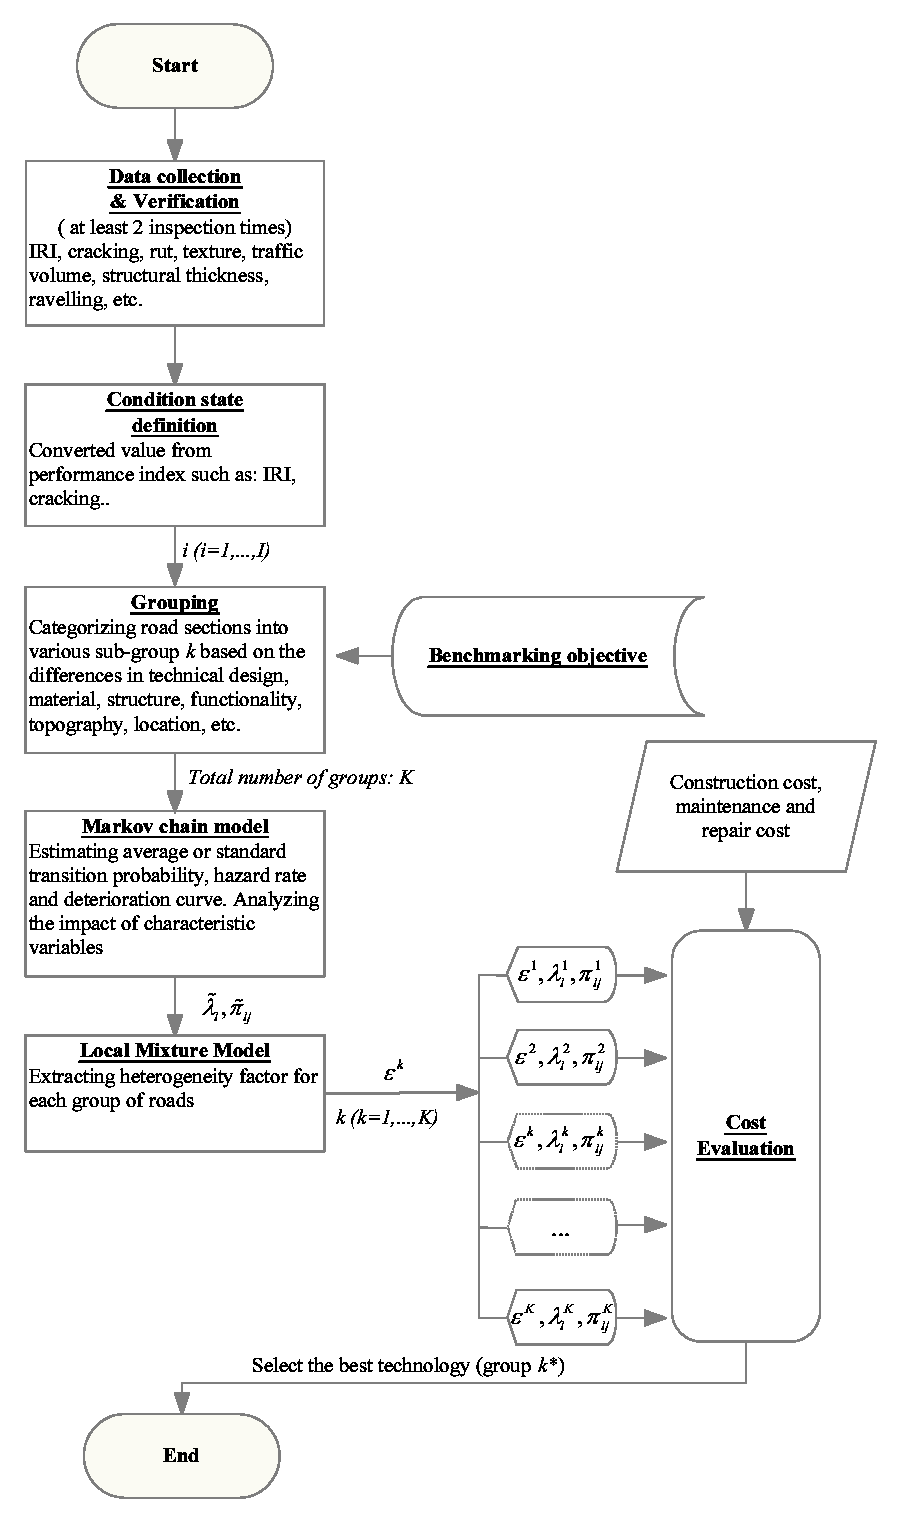
\includegraphics[scale=0.5]{fig62} 
\end{center}
\caption{Benchmarking Flowchart in PMS}
\label{fig62} 
\end{figure}
%%
\section{Empirical study}
\label{66}
\subsection{Overview of empirical study}
\label{661}
In this section, we exploit the applicability of the exponential hazard model to estimate the Markov transition probability. Further, the heterogeneity factor of individual road group is estimated by using the mixture model. Benchmarking study is highlighted with the comparison of deterioration curves. Empirical application is conducted on the monitoring data of the national road system in Vietnam. There are over $10,000$ samples in the database. Each sample represents a road section of 1 km in length. After verification, a sampling population during the period from $2001$ to $2004$ with $6510$ road sections is selected for the empirical test. Information of monitoring data includes the values of indexes such as: International Roughness Index (IRI), Cracking, Texture depth, Thickness of top asphalt layer, Annual traffic volume, etc. The locations of examined road sections are mapped in Figure \ref{fig63}.

In benchmarking study, we consider the deterioration of top surface layers characterizing by type of materials, technical specification, and regional differences. Whilst, the traffic volume and texture depth are considered as characteristic variables. A main reason of the selection is because of having a wide range of choices in the practices of design, construction, and maintenance in Vietnam. In other words, most of pavement technologies are borrowed technologies from developed nations, causing a pavement system of inhomogeneous conditions. The problem of having inhomogeneous conditions in the national pavement system consequently results in a negative influence on maintenance, repair, and renovation. The problem has been documented as a major difficulty for budget allocation either in short or long term strategy.

The original set of monitoring data is filtered and verified in order to define an appropriate range of condition states. Verification 
is necessary since the range of condition states can be converted in various domains from the value of distress. In fact, the values of distress such as Roughness, Cracking, Flatness, and Rut are measured and recorded in a very small scale. Thus, the requirement for defining the range is extremely important. Based on the results of data verification, we realize that the arrival time to the worst condition state are in similar behaviors if different range of condition states are assumed. Hence, for the convenience of observation and computation, we select the range of condition states from $1$ to $5$ as detailed described in Table \ref{table61}. The range of condition states is converted values from the value of IRI.  

\begin{figure}[t]
\begin{center}
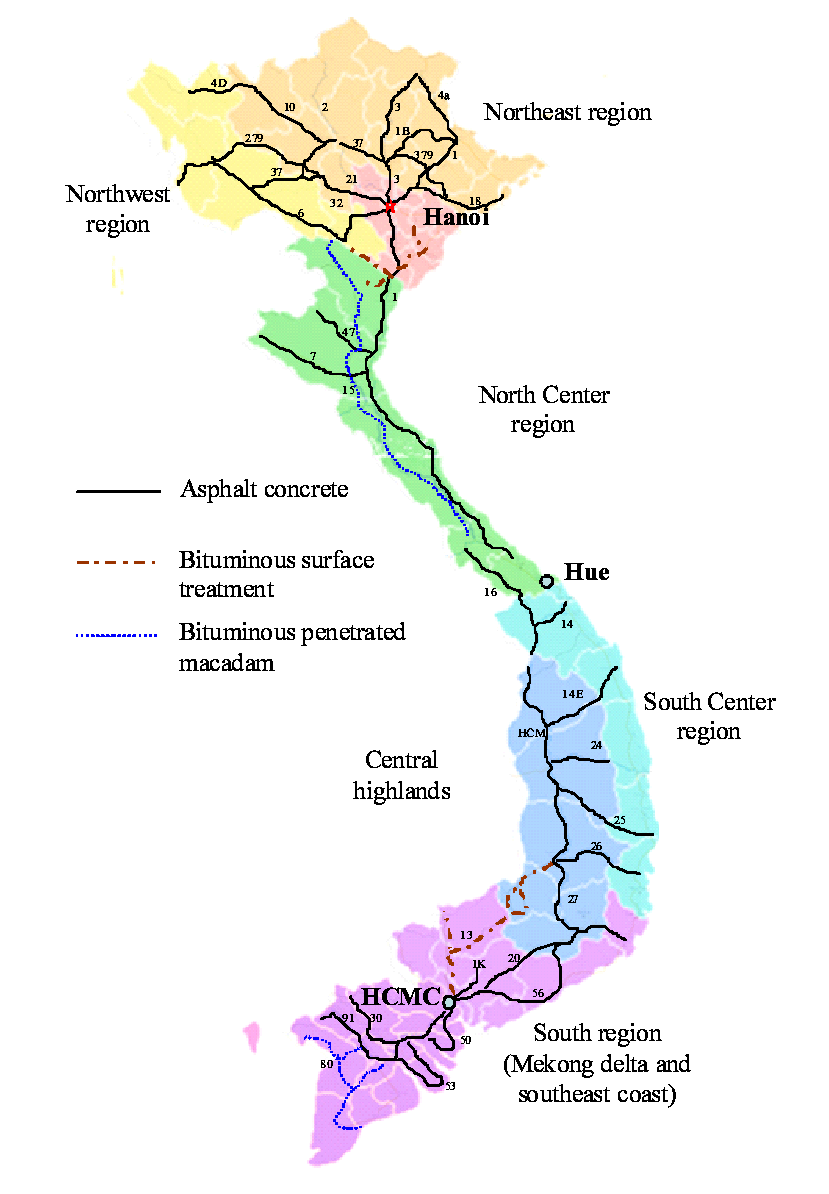
\includegraphics[scale=0.6]{fig63}
\end{center}
\footnotesize Note)  Numbers on the map are the names of national roads.
\caption{Locations of Roads.}
\label{fig63}
\end{figure}

%%%
\begin{table}[t]
\caption{Description of Condition States.}
\label{table61}
{\small
\begin{center}
\begin{tabular}{c|c|c}\hline
Condition states & Range of IRI values & Remark\\\hline
1 & (1-2] & Very good\\
2 & (2-4] & Good \\
3 & (4-6] & Fair \\
4 & (6-8] & Poor \\
5 & $>$ 8 & Very poor \\\hline
\end{tabular}
\end{center}
}
\footnotesize Note) IRI is measured in (m/km).
\end{table}%[t]
\subsection{Estimation results}
\label{662}

In the empirical study, we consider the annual traffic volume of motorized car and the change of texture index as characteristic variables, with denotations as $x_{i2}$ and $x_{i3}$. While, the first characteristic variable $x_{i1}$ equals to 1 as a constant value. The thickness of pavement is not considered in the estimation because it shares a similar range of value in design practices.

Estimation results using the exponential Markov model are displayed in Table \ref{table62}. It is highlighted from the table that the traffic volume has a great influence on the transition of condition state $4$. A strong correlation between the transition of the first two condition states $(i=1,2)$ and the texture depth is also realized. As a matter of fact, the change in the texture depth of road depends on the traffic volume and other environmental conditions such as climate and construction materials. The figures displayed in the parenthesis represent the statistical $t-test$ for the values of unknown parameters.

\begin{table}[t]
\begin{center}
\caption{Estimation Results of Exponential Hazard Model.}
\label{table62}
{\small
\begin{tabular}{c|c|c|c}\hline
Condition & Constant&Traffic volume &Texture depth\\
 states & $\beta_{i1}$ & $\beta_{i2}$& $\beta_{i3}$\\ \hline
1 & 0.7987  &  - &  - \\
& (46.633) & -  &  -\\\hline
2 & 0.004 &  -  &  1.9633 \\\
& (0.547) &  - &  (21.042)\\\hline
3 & 0.225  &  - &  -\\
& (29.629) & - &  -\\\hline
4 & 0.0849 &  3.0108 &  -\\
& (5.8440) &(5.9501)&  -\\\hline
\end{tabular}
}
\end{center}
\footnotesize Note) $t-$ values are shown in the parenthesis.
\end{table}

Eventually, we obtain the values of hazard rate and life expectancy for condition state $i$ through equations (\ref{hazard1}) and (\ref{17}). Results are presented in Table \ref{table63}. It is highlighted that, in average, the life expectancy of condition state $i=1$ lasts less than $1.5$ years before entering into condition state $i=2$. Condition states $2$ has its service life about $5.5$ years. After entering condition state $i=3$, the speed of deterioration accelerates in a fast manner. For instance, condition state $3$ remains only about $4.5$ years before falling to condition state $i=4$. And further, it takes less than $3.5$ years for condition state $i=4$ arriving to the absorbing condition state $(i=5)$.

\begin{table}[t]
\caption{Life Expectancy of Condition States.}
\label{table63}
\begin{center}
{\small
\begin{tabular}{c|cc}\hline
   Condition states& ~$E[\theta_{i}]$~& $E[RMD_{i}^k]$(years) \\\hline
  1 & ~0.7987~ & ~1.2521  \\
   2 & ~0.1835~ & ~5.4488  \\
   3 & ~0.2252~ & ~4.4401 \\
   4 & ~0.2901~ & ~3.4474 \\
   \hline
\end{tabular}
}
\end{center}
\footnotesize Note) The values of hazard rate and life expectancy are not defined for the  absorbing condition state ($i=5$) in Markov chain model.
\end{table}

\begin{table}[t]
\caption{Markov Transition Probability.}
\label{table64}
\begin{center}
{\small
\begin{tabular}{l|lllll}
\hline
\multicolumn{1}{c|}{Condition} & \multicolumn{5}{c}{Condition states} \\ 
\multicolumn{1}{c|}{states} & \multicolumn{1}{c}{1} & \multicolumn{1}{c}{2} & \multicolumn{1}{c}{3} & \multicolumn{1}{c}{4} & \multicolumn{1}{c}{5} \\ 
\hline
\multicolumn{1}{c|}{1} & \multicolumn{1}{c}{0.4499} & \multicolumn{1}{c}{0.4965} & \multicolumn{1}{c}{0.0495} & \multicolumn{1}{c}{0.0038} & \multicolumn{1}{c}{0.0003} \\ 
\multicolumn{1}{c|}{2} & \multicolumn{1}{c}{0.0} & \multicolumn{1}{c}{0.8323} & \multicolumn{1}{c}{0.1496} & \multicolumn{1}{c}{0.0164} & \multicolumn{1}{c}{0.0017} \\ 
\multicolumn{1}{c|}{3} & \multicolumn{1}{c}{0.0} & \multicolumn{1}{c}{0.0} & \multicolumn{1}{c}{0.7983} & \multicolumn{1}{c}{0.1741} & \multicolumn{1}{c}{0.0276} \\ 
\multicolumn{1}{c|}{4} & \multicolumn{1}{c}{0.0} & \multicolumn{1}{c}{0.0} & \multicolumn{1}{c}{0.0} & \multicolumn{1}{c}{0.7482} & \multicolumn{1}{c}{0.2518} \\ 
\multicolumn{1}{c|}{5} & \multicolumn{1}{c}{0.0} & \multicolumn{1}{c}{0.0} & \multicolumn{1}{c}{0.0} & \multicolumn{1}{c}{0.0} & \multicolumn{1}{c}{1.0} \\ 
\hline
\end{tabular}
}
\end{center}
\footnotesize Note) The values of hazard rate and life expectancy are not defined for the  absorbing condition state ($i=5$) in Markov chain model.
\end{table}

\begin{figure}[t]
\begin{center}
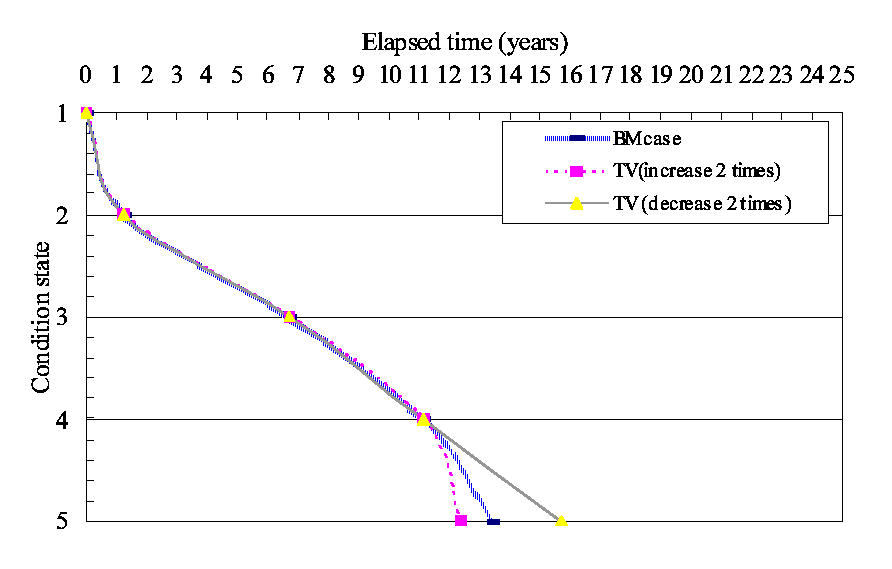
\includegraphics[scale=0.55]{fig64}
\end{center}
\caption{Deterioration Curve.}
\label{fig64}
\end{figure}

The matrix of Markov transition probability, estimated by using the exponential Markov model, is displayed in Table \ref{table64}. The values of transition properties are estimated based on the value of average hazard rate, which represents the deterioration transition pattern of the entire road sections. In order to compare the influence of traffic volume on the deterioration, we carry out the estimations for three cases. The benchmark (BM) case refers to the case that we estimated the hazard rates and transition probability based on annual traffic volume. Whilst, other two cases consider the increase and decrease of annual traffic volume at the rate $0.5$. Comparative results of three cases are illustrated in Figure \ref{fig64}.

An appealing conclusion from Figure \ref{fig63} is that the traffic volume particularly exerts to have a high impact on condition state $4$. In fact, it is true to accept that the traffic volume should affect all the condition states with different severe levels. However, in order to understand its behavior precisely, a richer database of monitoring data is required. Despite the limitation of monitoring data, we are still able to give an alarming message that the deterioration of the road network in Vietnam is progressing with a high speed of deterioration. The life expectancy of the surface layer in the network is relatively less than $13$ years. Probabilistically, after about $6$ years from construction time, the serviceability of the road network cannot satisfy the expectation of users. Thus, it is strongly recommended that Vietnamese road administration should proposes an extensive investigation to find out the causes of high deterioration speed, and works out a suitable plan to prolong the service life of the entire road network.
%%%%%%%%%%%%
\subsubsection{Heterogeneity distribution and deterioration curves}
\label{6621}

\begin{table}[t]
\begin{center}
\caption{Grouping Classification of Roads.}
\label{table65}
{\footnotesize
\begin{tabular}{c|l|c|c|c|c}\hline
   Group& Description & Technical & Speed & Road & Functional  \\
      k  &   & class & flow & class & class \\\hline
   1 & ~Bituminous penetrated macadam~(226) & ~60 & 3+4 & 1 & 3   \\
   2 & ~Bituminous surface treatment~(1301) & ~60 & 1+3+4 & 1+2 & 3+4+5   \\
   3.1 & ~Asphalt concrete ~(713) & ~40 & 4 & 1 & 4   \\
   3.2 & ~Asphalt concrete ~(1047) & ~60 & 3 & 2 & 2  \\
   3.3 & ~Asphalt concrete ~(1030) & ~60 & 3 & 1 & 3  \\
   3.4 & ~Asphalt concrete ~(467) & ~60 & 3 & 1 & 4  \\
   3.5 & ~Asphalt concrete ~(602) & ~60 & 3 & 2 & 3    \\
   3.6 & ~Asphalt concrete ~(1025) & ~80 & 3 & 1 & 2   \\
   3.7 & ~Asphalt concrete (99)~ & ~60 & 4 & 1 & 3  \\
  \hline
\end{tabular}
}
\end{center}
\footnotesize Note) Figures in the parenthesis shows number of data. Technical class is defined by maximum allowance speed used in design. Speed flow is categorized in the range (\textbf{1}-single lane with width $<=$3.5m; \textbf{2}-3 lanes with width of 10-14.5 m; \textbf{3}-2 lanes with width of 3.5-5.5 m; \textbf{4}-2 lanes with width of 5.5-10.5m; \textbf{5}- 4 lanes with width $>=$ 14m). Road class \textbf{1} refers to main tracks of national roads, \textbf{2} is supplement tracks of national roads. Functional class refers to management level \cite{tcvn4054}. Group 1 and 2 are classified with a combination of several designated factor.
\end{table}

In the benchmarking study, we categorize $6510$ road sections into three groups according to the types of materials. In addition, we further classify the group of asphalt concrete materials into seven smaller groups based on the technical class, speed flow, road class, and functional class since this group accounts for a large number of samples in monitoring data. Thus, the total number of groups are nine, with the detailed description explained in Table \ref{table65}. The locations of roads belonging to each group are also highlighted in Figure \ref{fig62}. Estimation results for heterogeneity factor of individual group by employing both parametric and semi-parametric approaches are also given in Figure \ref{fig64} and Figure \ref{fig65}. 

\begin{figure}[t]
\begin{center}
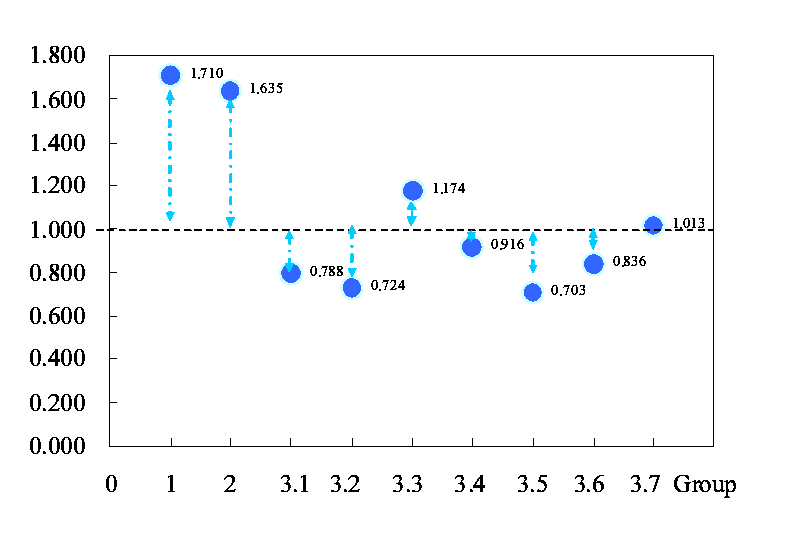
\includegraphics[scale=0.5]{fig65}
\end{center}
\caption{Distribution of Heterogeneity Factors - Parametric Approach.}
\label{fig65}
\end{figure}

\begin{figure}[t]
\begin{center}
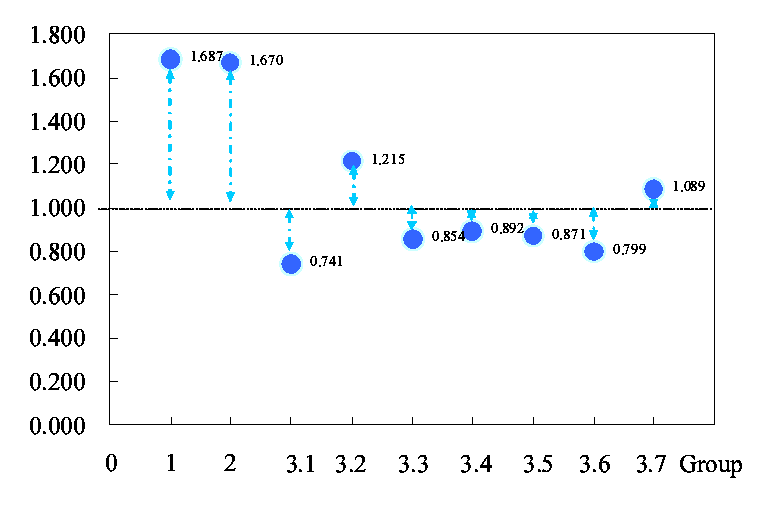
\includegraphics[scale=0.5]{fig66}
\end{center}
\caption{Distribution of Heterogeneity Factors - Semi-parametric Approach).}
\label{fig66}
\end{figure}

Comparisons of deterioration curves are drawn in Figure \ref{fig67} with parametric approach and in Figure \ref{fig68} with semi-parametric approach. The figures shows the deterioration curves of roads based on $3$ types of materials. The group of roads with asphalt overlays has a longest service life (about 16 years). Meanwhile, the two other groups of roads with materials composing of bituminous penetrated macadam and bituminous surface treatment have their service life less than $9$ years. Since asphalt concrete becomes a popular material for overlay, most of national roads are now paved with asphalt concrete. Thus, we further classified the group of asphalt concrete into $7$ sub-groups and compared their deterioration curves. In total, there are nine groups of roads for benchmarking. Figure \ref{fig69} and Figre \ref{fig610} presents the a comparative view on the deterioration curves of $9$ groups. It is realized that deterioration curves of asphalt concrete surfaces has a small dispersion in compare with other groups. Relatively, the life expectancy of asphalt concrete surfaces ranges from $12$ to $16$ years.

\begin{figure}[t]
\begin{center}
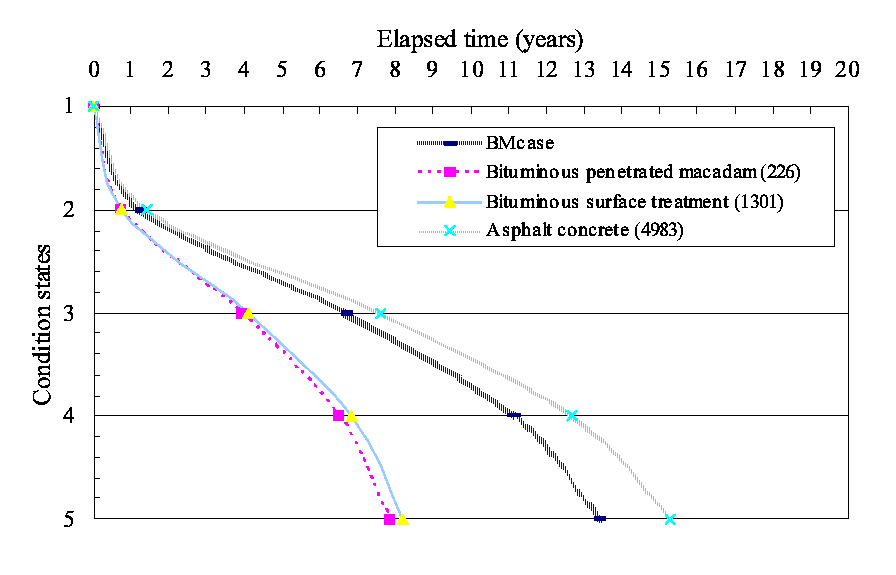
\includegraphics[scale=0.5]{fig67}
\end{center}
\caption{Deterioration Curves - 3 Types of Road Materials - Parametric approach.}
\label{fig67}
\end{figure}

\begin{figure}[t]
\begin{center}
\includegraphics[scale=0.5]{fig68}
\end{center}
\caption{Deterioration Curves - 3 Types of Road Materials - Semi-parametric Approach.}
\label{fig68}
\end{figure}
%
%
\begin{figure}[t]
\begin{center}
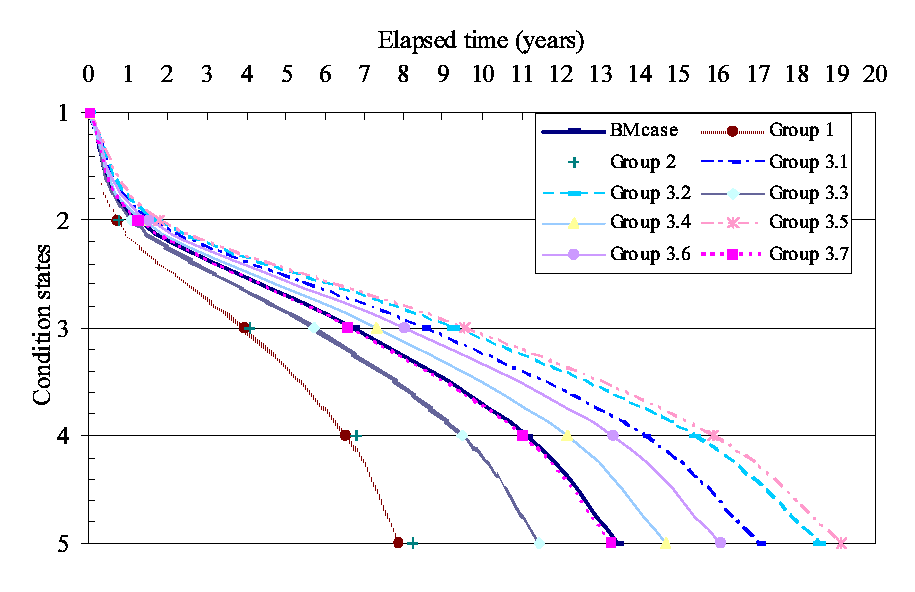
\includegraphics[scale=0.5]{fig69}
\end{center}
\caption{Deterioration Curves-9 Groups - Parametric Approach.}
\label{fig69}
\end{figure}

\begin{figure}[t]
\begin{center}
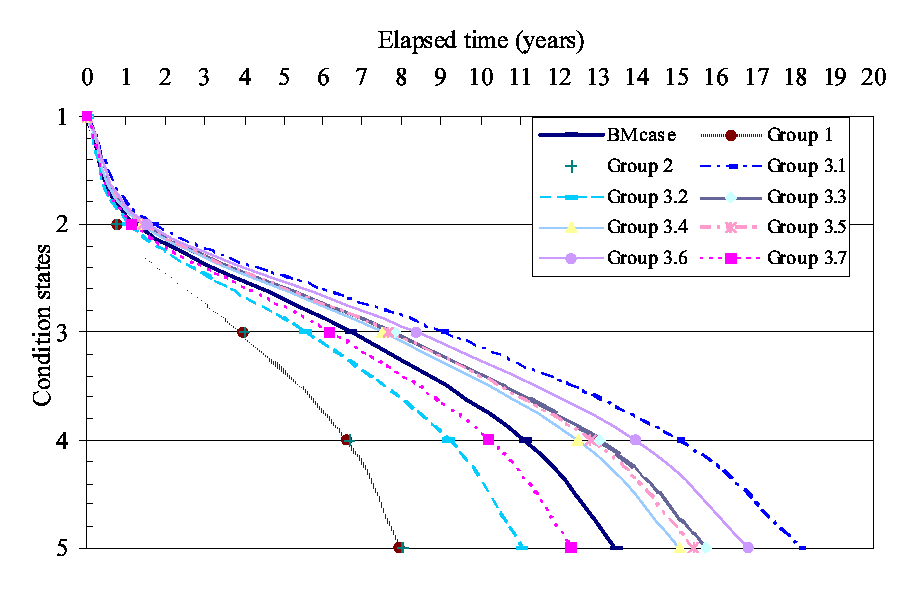
\includegraphics[scale=0.5]{fig610}
\end{center}
\caption{Deterioration Curves-9 Groups - Semi-parametric Approach).}
\label{fig610}
\end{figure}
\begin{figure}[t]
\begin{center}
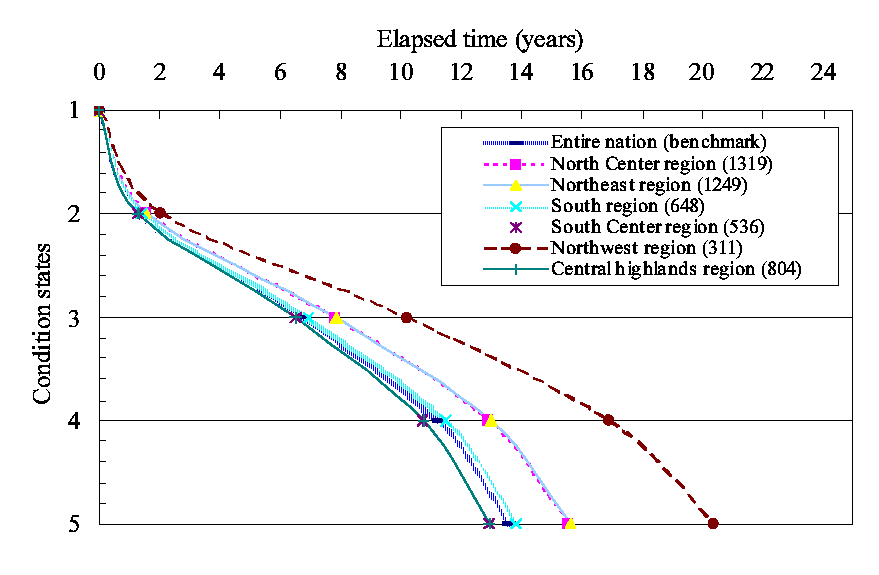
\includegraphics[scale=0.5]{fig611}
\end{center}
\caption{Deterioration Curves-regional Perspective (6 regions) - Parametric  Approach.}
\label{fig611}
\end{figure}
%%
\begin{figure}[t]
\begin{center}
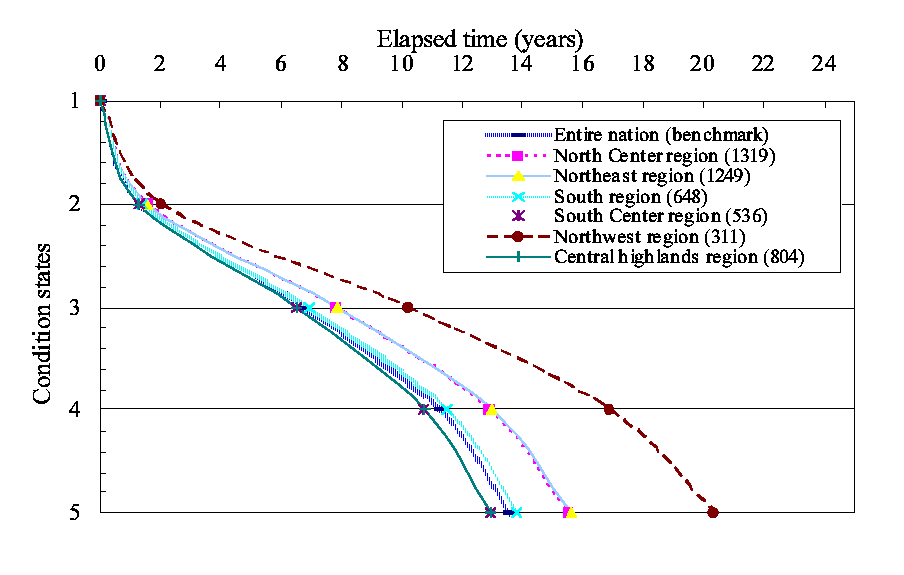
\includegraphics[scale=0.5]{fig612}
\end{center}
\caption{Deterioration curves-Deterioration Curves - Regional Perspective (6 regions) - Semi-parametric Approach.}
\label{fig612}
\end{figure}

According to the climate zones of Vietnam, road sections with asphalt concrete overlay are classified into $6$ regions. The location of each region is also displayed in the map of Figure \ref{fig63}. A comparative view of the deterioration curves of asphalt roads according to regional classification are illustrated in Figure \ref{fig611} and Figure \ref{fig612}. As can be seen from two figures, it is proved that the deterioration of road surfaces in the southern part is faster than that of road surfaces in the northern regions. This reason could possibly due to the effects of soft ground condition in the southern part of Vietnam or the impact of flooding in low land areas. The two prominent reasons are strongly believed to cause the subsidence of construction works in the southern part of the country. The deterioration of road surfaces in the north part of the country has a slower speed than the that of the other regions. Moreover, it is also found that that deterioration speed of road surfaces in urban areas is faster than that in the highland regions. The faster deterioration speed in the urban areas is due to the effects of heavier traffic volume annually.

Throughout the analysis and comparison of estimation results as presented in the above figures, it is realized that the there exists variations of estimation results between two methodologies (Parametric and Semi-parametric). However, the variations are observed in a small scale. Thus, the two approaches can be supplementary used for each other in order to improve the quality of estimation.
%
%%%
\subsubsection{Cost Evaluation}
\label{6622}
In view of economic evaluation, a simple cost evaluation technique is applied. We assumed that whenever the condition state of a road section reaching the absorbing state $(i=5)$, renewal will be implemented. The total cost is a summation of construction cost and renewal cost for renewing the overlay. With this assumption, the average cost of construction and renewal for each type of road surface according to its material can be estimated, simply by calculating the ratio of its total cost to its average life expectancy. 

The results of cost estimation are presented in Table \ref{table66}. The results highlight the fact that higher benefit can be earned if the asphalt concrete overlay is applied instead of applying the bituminous penetrated macadam and bituminous surface treatment overlays. A significant difference in the life expectancy and average cost within the group of asphalt concrete material is also realized from the estimation results in Table 6. Based on the obtained results, the best type of overlay for long term application can be recommended. For example, group 3.1 in Table \ref{table66} is considered as the best one in term of economic perspective. 

\begin{table}%[t]
\begin{center}
\caption{Average Cost Evaluation.}
\label{table66}
{\small
\begin{tabular}{c|c|c|c}\hline
   Group&  Renewal & Service & Average \\
      k  & cost  & life (years)  & cost \\\hline
   1 &  ~8,567 & 7.64   & 1,121 \\
   2 &  ~8,929 & 7.72    & 1,157 \\
   3.1 &  ~11,754 & 17.38   & 676 \\
   3.2 &  ~11,754 & 10.61   & 1,108 \\
   3.3 &  ~11,754 & 15.09  & 779 \\
   3.4 &  ~11,754 & 14.45   & 814 \\
   3.5 &  ~11,754 & 14.79   & 795 \\
   3.6 &  ~11,754 & 16.12   & 729 \\
   3.7 &  ~11,754 & 11.84   & 993 \\
   \hline
\end{tabular}
}
\end{center}
{\small Note) Monetary unit is $1000$ thousand Vietnamese dong. Unit cost is referred to the standard norm cost defined by Hanoi construction bureau \cite{dghanoi08,dm1242}. Cost is estimated for 100 $m^2$ and 5 cm in its thickness of road.}
\end{table}
%
%
% Deterioration curve with respect to each hetegoneity factor 
\section{Summary and Recommendations}
\label{67}
This chapter has proposed a mixture model for benchmarking study. The mixture model is expressed by means of heterogeneity factor $\epsilon$ that exists in each group of roads. The heterogeneity factor is considered to follow the Gamma distribution (Parametric approach) and the function of Taylor series (Semi-parametric approach). In order to estimate the heterogeneity factor, two steps estimation approach with maximum likelihood estimation method is applied. The mixture hazard model is considered as an excellent tool for benchmarking study, which is used to search for the best technology in the pavement management system. In view of practical application, the methodology is suitable to apply in the pavement management system of developing countries like Vietnam, where has a high demand of standardization in the pavement system.

To demonstrate the applicability of the model, we conducted an empirical study on a database of Vietnamese pavement system collected during the years $2001$ and $2004$. The technological groups were classified according to the types of materials and regional zones. The estimation results revealed a fact that the speed of deterioration of roads in Vietnam is very fast. Approximately $10$ years after construction, the condition states of road surfaces reach the worst condition state. The main cause leading to the fast deterioration is because of the high intensity of annual traffic volume. Furthermore, estimation results prove that the performances of road surfaces with asphalt concrete are much better than that of the road surfaces with bituminous penetrated macadam and bituminous surface treatment. Based on a simple cost evaluation technique, the empirical study also recommended a best group of road surfaces with asphalt concrete for long term application. 

However, we have not discussed several points, which will be considered as topics for extending this study in the future:

\begin{itemize}
\item The benchmarking study focused only on the pavement management system. However, its application can be applied to other types of infrastructure.
\item This chapter proposed only a simple cost evaluation technique, which does not considered the routine maintenance and repair actions. In order to overcome this limitation, a cost evaluation technique using the theory of Markov decision process should be applied in the future extension of the model.
\item This chapter has not discussed the problem of measurement errors in monitoring data, which is one of the main reason causing the bias in estimation results. A future study shall consider the theory of hidden Markov models, Bayesian estimation, and Markov Chain Monte Carlo into account.
\item The empirical study of this chapter just focused on a small scale application of benchmarking methodology on the pavement system in Vietnam, particularly focusing on the types of materials and regional zones. However, in order to find out the best pavement technology and to propose a feasible solution to the problems of pavement system in Vietnam, a better quality monitoring data shall be accumulated.
\item In the empirical study, we considered only the annual traffic volume as a time-invariant characteristic variable. However, in reality, the intensity of annual traffic volume is always dynamic and change with time. Therefore, it is recommended that future extension of the study shall consider the traffic volume as a time-variant characteristic variable.
\end{itemize}

\section{General introduction}
\label{61}
The statistical hazard models based on the visual inspection data have been widely practiced in the field of infrastructure asset management. In the models, Markov chain theory with it presumption of accuracy and generality to real data has been usefully applied. Furthermore, with use of Markov decision process, decision making process can gain the advantage for management of infrastructure system, especially at strategic and macroscopic level.
 
In addition to the decision making process at strategic level, it is necessary to develop a model which can be applied to generate information for various levels. For example, in bride management, a concrete maintenance plan for some important individual components is important; this plan can be regarded as for ``component level''. In fact, deterioration processes of individual components under the same structural characteristic and an environmental condition are also different. Therefore, in order to develop a more exquisite deterioration forecast technique, it is acknowledged to consider the heterogeneity of the deterioration process of individual components which are under the same structural characteristic and environmental condition. This Markov deterioration hazard model differs from the model, which also employs Markov transition probability based on the total of huge deterioration information and average deterioration process.

However, in fact, there is obvious not much comprehensive study on Markov deterioration model that pays great attention on the heterogeneity of the deterioration process. These might due to constrains like facing accuracy and efficiency of collected information, increasing work load of business and management...etc, which limited previous studies on establishing sound assumptions to heterogeneity factor. Therefore, the development of a more efficient deterioration forecast technique in consideration with the heterogeneity of the deterioration process is mandatory.

The favor for mixture model and benchmarking approach is further rendered by the quest for the selection of best pavement technology, particularly based on material, structure and construction technique. This quest is realized in high attention, especially in the developing nations \cite{kcleong}. Therefore, beside the analytical method for mixture model, this chapter extends its words on benchmarking study. 

A good example of benchmarking application is the case of Vietnam, where the entire road system is comprised of many different technologies. Reason to this is, as the matter of fact, due to limited capacity, the country often borrowed technologies from abroad. National standards for design and construction practices are somewhat mimic versions of guidelines, most of them are copied from developed nations. This practice is definitely unlike to that of developed nations. Consequently, leads to huge amount of efforts and budget in monitoring and maintenance during operation phases. Hence, in view of long term and strategic management, there is a strong demand in searching for the best pavement technology, which could become a national standard in pavement management system. 

%%%%%%%%%%%%%%%%%%%%5
\section{Heterogeneity and Sampling Population}
\label{62}
As a matter of fact, deterioration speed of one infrastructure component is always different from the other even thought they share the same structural characteristics. This is due to the fact that each component bears different working environment from the other. For instance, the cracking rate of pavement section often contains some degree of variation from each other even they belongs to a short distance road length. With respect to the deterioration speed of the infrastructure with similar characteristics, it is often the case that, only representing deterioration curve is drawn in connection to average hazard rate. Without any exception, Markov hazard model is used to estimate this average value. In a broaden understanding, suffice to say that the average value of hazard rate is actually added or weighted by individual hazard rate of each component or each group of similar component. 

Probabilistically, hazard rate of individual component is distributed around the mean of average value. An illustration of this situation is sketched in Figure \ref{fig61}. As can be seen from the figure, at time $\tau_i$ the estimated condition state from forecasting model is $i$. However, deterioration speed of individual can be either faster or slower than the average curve as showed in dotted lines.
%
\begin{figure}[t]
\begin{center}
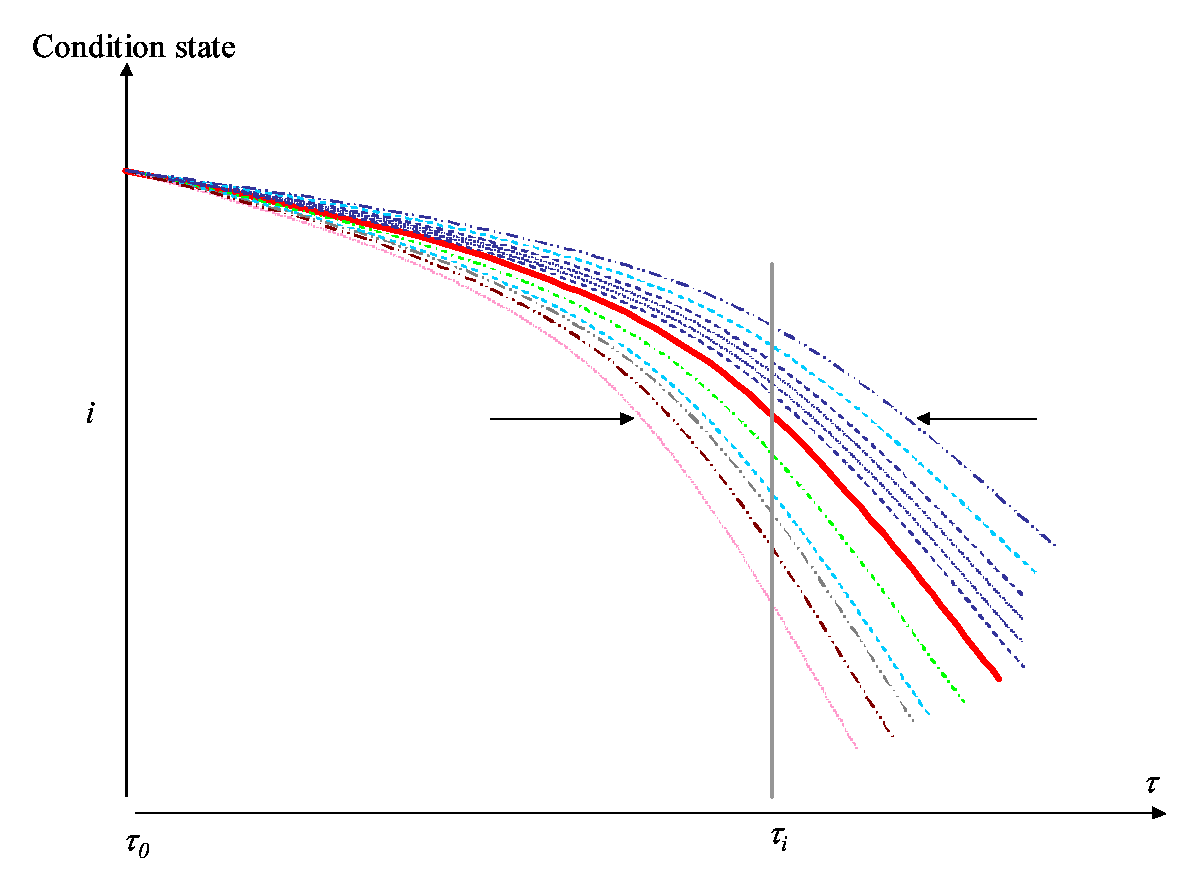
\includegraphics[scale=0.5]{fig61} 
\end{center}
\footnotesize Note) Each line represents for deterioration curve of individual road section or group of road sections with similar characteristics.
\caption{Deterioration curve differences.}
\label{fig61} 
\end{figure}
%
%%%%%%%%%%%%%%%%%5
\section{Mixture Markov deterioration hazard model}
\label{64}
\subsection{Markov transition probability and heterogeneity factor}
\label{641}
In reality, deterioration process varies differently among pavement groups due to dynamic factors. Thus, it is hard to grant a homogeneous sampling population in estimation. To express this inhomogeneous sampling population, many literatures in liability modeling employ the term ``heterogeneity factor''. In pavement system, we assume the entire road system comprising of $K$ group of road according to their technological difference. In each group $k (k=1,...,K)$, total road section is $S_k$. And $\varepsilon^k$ is referred as the heterogeneity factor, which infers the change of characteristic of a peculiar hazard rate $i(i=1,...,I-1)$ to a pavement section $s_k(s_k=1,\cdots,S_k)$. Thus, the mixture form of hazard function, which mentioned in equation (\ref{hazard}) of Chapter \ref{Chapter2}, can be defined:
\begin{eqnarray}
&& \lambda_i^{s_k} = \tilde{\lambda}_i^{s_k}\varepsilon^k \hspace{5mm}
 (i=1,\cdots,I-1;k=1,\cdots,K;s_k=1,\cdots,S_k).  \label{hu1}
\end{eqnarray}
$\varepsilon^k$ is always non-negative. In addition, it is understood that the higher value of $\varepsilon^k$ is, the faster deterioration speed of road section $s_k$ comparing to others. Within the one group of road sections (or one technology), the hazard rate of all ratings holds the same the value of the heterogeneity factor $\varepsilon^k$. Counting all the road sections as a whole, the distribution of $\varepsilon^k$ is exactly representing the influence of individual group of road sections on the overall deterioration process. Depending on structural characteristic of each system, heterogeneity factor $\varepsilon^k$ can be in form of a function or stochastic variable.

For measurable representation, we denote a set of value of $\varepsilon^k$ $(k=1,..,K)$ as a vector $\bar{\varepsilon}^k$. The bar [$\bar {\hspace{2mm}}$] indicates measurable value. As a result, we can further expressed the survival probability in equation (\ref{prop-bFla}) by means of mixed hazard rate in equation (\ref{hu1}) for pavement group $k$:
\begin{eqnarray}
&& \tilde{F}_i(y_i^{k})=\exp(-\tilde{\lambda}_i\bar{\varepsilon}^k y_i^k) .\label{prop1}
\end{eqnarray}
Siminarly, Markov transition probability expressed in equations (\ref{p1})-(\ref{pj}) are derived as follows:
\begin{manyeqns}
&& \pi_{ii}^k(z^k:\bar{\varepsilon}^k)=\exp(-\tilde{\lambda}_i^k\bar{\varepsilon}^k z^k), \label{prop2}\\
&& \pi_{ij}^k(z^k:\bar{\varepsilon}^k)=\sum_{l=i}^{j}
\prod_{m=i,\neq l}^{j-1}\frac{\tilde{\lambda}_m^k}{\tilde{\lambda}_{m}^k-\tilde{\lambda}_{l}^k} \exp (-\tilde{\lambda}^{k}_l\varepsilon^k z^k)\nonumber\\
&& \hspace{10mm} =\sum_{l=i}^{j}\psi_{ij}^l(\tilde{\mbox{\boldmath$\lambda$}}^k) \exp (-\tilde{\lambda}_{l}^k \varepsilon^k z^k) \label{poi1}\\
&& (i=1,\cdots,I-1;j=i+1,\cdots,I;k=1,\cdots,K), \nonumber
\end{manyeqns}
where
\begin{eqnarray}
&& \psi_{ij}^l(\tilde{\mbox{\boldmath$\lambda$}}^k)=
\prod_{m=i,\neq l}^{j-1}\frac{\tilde{\lambda}_m^k}{\tilde{\lambda}_{m}^{k}-\tilde{\lambda}_{l}^k}. \label{psi}
\end{eqnarray}
\subsection{Parametric approach to heterogeneity factor $\varepsilon$}
\label{642}
In parametric approach, the heterogeneity factor $\varepsilon^k$ is assumed as a probability sample extracted from Gamma distribution $f(\varepsilon^k:\alpha,\gamma)$:  
\begin{eqnarray}
&& f(\varepsilon^k:\alpha,\gamma)=\frac{1}{\gamma^\alpha \Gamma(\alpha)}\left(\varepsilon^k\right)^{\alpha-1}\exp\left(-\frac{\varepsilon^k}{\gamma}\right). \label{gamma}
\end{eqnarray}
Gamma distribution $f(\varepsilon:\alpha,\gamma)$ has its mean $\mu=\alpha.\gamma$ and standard variance $\sigma^2=\alpha.\gamma^2$. In addition, if $\alpha=1$, it turns to be exponential distribution. For handy calculation in the following writings, the mark $k$ is temporary omitted. The life expectancy of condition state $i$ keep unchanging until or more than the time $y_i$ in equation \ref{prop1} is actually the transition probability $\pi_{ii}$:
%%%%%%%%%%
\begin{eqnarray}
&& \tilde{\pi}_{ii}(z)=\int_0^\infty \pi_{ii}(z:\varepsilon)f(\varepsilon:\alpha,\gamma)d\varepsilon \nonumber \\
&& \hspace{5mm} =\int_0^\infty \exp(-\tilde{\lambda}_i\varepsilon z)
\frac{1}{\gamma^\alpha \Gamma(\alpha)}\varepsilon^{\alpha-1}\exp\left(-\frac{\varepsilon}{\gamma}\right)d\varepsilon \nonumber \\
&& \hspace{5mm}=\frac{1}{\gamma^\alpha \Gamma(\alpha)}\int_0^\infty \exp\left\{\left(-\tilde{\lambda}_i z-\frac{1}{\gamma}\right)\varepsilon\right\}\varepsilon^{\alpha-1}d\varepsilon \nonumber\\
&& \hspace{10mm}(i=1,\cdots,I-1) . \label{prp11}
\end{eqnarray}
%%%%%%%%%%%%%%%%%%%%%

By setting $u_i=(\tilde{\lambda}_i z+\frac{1}{\gamma})\varepsilon$, equation \ref{prp11} becomes
\begin{eqnarray}
&& \tilde{\pi}_{ii}(z)=\frac{1}{\gamma^\alpha \Gamma(\alpha)}\int_0^\infty \exp(-u_i)\left(\frac{u_i}{{\tilde{\lambda}_i z+\frac{1}{\gamma}}}\right)^{\alpha-1} 
 \frac{1}{{\tilde{\lambda}_i z+\frac{1}{\gamma}}} du_i \nonumber \\
&& \hspace{3mm}=\frac{1}{\gamma^\alpha \Gamma(\alpha)}\left(\frac{1}{{\tilde{\lambda}_i z+\frac{1}{\gamma}}}\right)^\alpha \int_0^\infty \exp(-u_i)u_i^{\alpha-1}  du_i \nonumber \\
&& \hspace{3mm}=\frac{1}{\gamma^\alpha \Gamma(\alpha)}\left(\frac{1}{{\tilde{\lambda}_i z+\frac{1}{\gamma}}}\right)^\alpha \Gamma(\alpha) 
=\frac{1}{(\tilde{\lambda}_i \gamma z+1)^\alpha}.
\end{eqnarray}
%%
In general case, the Markov transition probability of changing condition state from $i$ to $j$ under time interval $z$ will be
%%
\begin{eqnarray}
&& \tilde{\pi}_{ij}(z)=\int_0^\infty \pi_{ij}(z:\varepsilon)f(\varepsilon:\phi)d\varepsilon \nonumber \\
&& \hspace{5mm} = \int_0^\infty \sum_{l=i}^j \psi_{ij}^l(\tilde{\mbox{\boldmath$\lambda$}})\exp(-\tilde{\lambda}_l\bar{\varepsilon} z) f(\varepsilon:\alpha,\gamma) d\varepsilon \nonumber \\
&&  \hspace{5mm}=\sum_{l=i}^j \frac{\psi_{ij}^l(\tilde{\mbox{\boldmath$\lambda$}})}{\gamma^\alpha \Gamma(\alpha)}\int_0^\infty \exp\left\{\left(-\tilde{\lambda}_l z-\frac{1}{\gamma}\right)\varepsilon\right\}\varepsilon^{\alpha-1}d\varepsilon \nonumber \\
&& \hspace{5mm}=\sum_{l=i}^j\frac{\psi_{ij}^l(\tilde{\mbox{\boldmath$\lambda$}})}{(\tilde{\lambda}_l \gamma z+1)^\alpha}.
\end{eqnarray}
%%%
With existence of the heterogeneity factor $\varepsilon^k$, hazard rate of individual group is thought to be distributed as agreeing to average hazard rate $\tilde{\lambda}_i$. In this understanding, it is therefore assume for the Gamma distribution to have its mean of $1$ and standard variance of $1/\phi$. As a result, we can obtain the explicit form of Markov transition probability with respect to distribution of heterogeneity factor:
%%
\begin{manyeqns}
&& \tilde{\pi}_{ii}(z)=\frac{\phi^\phi}{(\tilde{\lambda}_i z+\phi)^\phi}, \label{ptpi410} \\
&& \tilde{\pi}_{ij}(z)=\sum_{l=i}^j \frac{\psi_{ij}^l(\tilde{\mbox{\boldmath$\lambda$}})\phi^{\phi}}{({\tilde{\lambda}_l z+\phi})^\phi}  ,\label{ptpi411} \\
&& (i=1,\cdots,I-1;j=i+1,\cdots,I) .\nonumber
\end{manyeqns}
%%%%%%%%
\subsection{Semi-parametric approach to heterogeneity factor $\varepsilon$}
\label{643}
A great deal of past research has revealed the difficulties in defining the heterogeneity factor $\varepsilon^k$. The assumption of the heterogeneity factor to be in the form of a function or a stochastic variable crucially depends on the characteristics of the system itself and the availability of monitoring data \cite{lancaster90,Marriott06}. This section focuses on applying mixture model in the case that the value distribution of heterogeneity factor $\varepsilon^k$ has a small dispersion. In other words, the departure of heterogeneity factor $\varepsilon^k$ from homogeneity is in a small scale. This type of mixture model is named as the local mixture model. In exponential family form $f(x;\epsilon)$ (where $x$ and $\epsilon$ are the variable and heterogeneity respectively), local mixing mechanism is defined via its mean parameterization $\delta^{k}$: 
%%%%
\begin{eqnarray}
g(x;\mu) : = f(x;\epsilon) + \sum_{i=2}^{r}f^{k}(x;\epsilon),\label{locami} 
\end{eqnarray}
where
\begin{eqnarray}
f^{k}(x;\epsilon)=\frac{\delta^{k}}{\delta\epsilon^{k}}f(x;\epsilon). \nonumber
\end{eqnarray}
%%%
Another class of the local mixture model that captures the behavior of scale dispersion in mixture value of function $f(x;\epsilon)$, is defined as the local scale mixture model.
\begin{eqnarray}
g(x;\epsilon) : = f(x;\epsilon) + \sum_{i=2}^{r}\frac{\epsilon^k}{k!}f^{k}(x;\epsilon). \label{localscal} 
\end{eqnarray}
Expansion of functions in equations (\ref{locami}) and (\ref{localscal}) can be seen to follow the Taylor series. Since the likelihood function of Markov transition probability in equations (\ref{locami}) and (\ref{localscal}) belongs to the exponential family. It is possible to approximate the transition probability as in the form of the local mixture distribution. 
%
\begin{eqnarray}
&& \tilde{\pi}_{ij}(z)=\int_0^\infty \pi_{ij}(z:\varepsilon)f(\varepsilon)d\varepsilon 
 (i=1,\cdots,I-1) . \label{prp12}
\end{eqnarray}
%
For convenience of mathematical manipulation, the local mixture transition probability is assumed as an exponential function $f_{mix}(\epsilon,z,\lambda)$ with $mix$ indicating the abbreviation of mixture. As the sequent, the mixture function $f_{mix}(\epsilon,z,\lambda)$ can be described by means of standard function $f(\epsilon,z,\lambda)$ and distribution $H(\varepsilon)$. Equation (\ref{prp12}) is further simplified as 
%%
\begin{eqnarray}
f_{mix}(\varepsilon,z,\lambda) = \int{f(\varepsilon,z,\lambda)}dH(\varepsilon), \label{prp2}
\end{eqnarray}
%
where $f(\varepsilon,z,\lambda)=exp(-\varepsilon\lambda z)$. Function $f(\varepsilon,z,\lambda)$ is likely a function of $\varepsilon$ about its mean. Without no loss of generality, and as long as the mean exist, we can further decompose equation (\ref{locami}) as follows:
\begin{eqnarray}
exp(-\varepsilon\lambda z)=e^{-\lambda z}(1+(\epsilon -1)(-\lambda z) 
+\frac{(\epsilon-1)^2}{2!}(-\lambda z)^2+ ... \hspace{2mm}.\label{taylor1}
\end{eqnarray}
This is the Taylor series. And thus, the quadratic form (when r = 2) is acceptable for an accurate approximation. Consequently, an explicit form of approximation can be derived for the Markov transition probability:
%
\begin{eqnarray}
E(e^{-\varepsilon\lambda z}) \approx e^{-\lambda z}\lbrace 1 + \frac{(\sigma\lambda z)^{2}}{2}\rbrace  \label{locfinal}
\end{eqnarray}
and
\begin{manyeqns}
&& \tilde{\pi}_{ii}(z) = e^{-\tilde{\lambda}_iz}\lbrace 1  + \frac{(\sigma\tilde{\lambda}_iz)^2}{2!}\rbrace, \label{piii} \\
&& \tilde{\pi}_{ij}(z) = \sum_{l = i}^j \psi_{ij}^l(\tilde{\mbox{\boldmath$\lambda$}})e^{-\tilde{\lambda}_lz}\lbrace 1 + \frac{(\sigma\tilde{\lambda}_lz)^2}{2!}\rbrace ,\label{piij}\\
&&(i=1,\cdots,I-1; j=i+1,\cdots,I). \nonumber
\end{manyeqns}

%%%%%%%%%%%%%%%%%%%%%%%%%%%%%%%%%%%%%%%%%%%%%%%%%%%%%%%%%%
\subsection{Likelihood estimation approach}
\label{644}
\subsubsection{Parametric estimation approach}
\label{6441}
\textit{a) Estimation assumtion}\\
%%%
The estimation of Markov transition probability and heterogeneity factor requires monitoring data from at least two visual inspections. Supposing that the periodical monitoring data of $S_k$ road sections is available. An inspection sample $s_k$ (a road section) implies two consecutive discrete periodical inspections at times $\bar{\tau}_A^{s_k}$ and $\bar{\tau}_B^{s_k}=\bar{\tau}_A^{s_k}+\bar{z}^{s_k}$, with its respective condition states $h(\bar{\tau}_A^{s_k})=i$ and $h(\bar{\tau}_B^{s_k})=j$. Based on monitoring data of $\sum_{k=1} ^K S_k$ samples, dummy variable $\bar{\delta}_{ij}^{s_k} ~ (i=1,\cdots,I-1,j=i,\cdots,I;s_k=1,\cdots,S_K;k=1,\cdots,K) $ is defined to satisfy the following conditions: 
%
 \begin{eqnarray}
      && \bar{\delta}_{ij}^{s_k}=\left\{
      \begin{array}{ll}
         1 &  h(\bar{\tau}_A^{s_k})=i,h(\bar{\tau}_B^{s_k})=j\\
         0 & Otherwise 
      \end{array}.
      \right.
   \end{eqnarray}
%
The range of dummy variable $(\bar{\delta}_{11}^{s_k},\cdots,\bar{\delta}_{I-1,I}^{s_k})$ is denoted by using the dummy variable vector $\bar{\mbox{\boldmath$\delta$}}^{s_k}$. Furthermore, structural characteristics and environment conditions of the road are expressed by means of characteristic variable vector $\bar{\mbox{\boldmath$x$}}^{s_k}=(\bar{x}_1^{s_k},\cdots,\bar{x}_M^{s_k})$, with $\bar{x}_m^{s_k}~(m=1,\cdots,M)$ indicating the observed value of variable $m$ for sample ${s_k}$. The first variable is referred as a constant term, with its value $x_1^{s_k}=1$. Thus, the information concerning monitoring data of sample $k$ can be described as $\mbox{\boldmath$\Xi$}^{s_k}=(\bar{\mbox{\boldmath$\delta$}}^{s_k},\bar{z}^{s_k},\bar{\mbox{\boldmath$x$}}^{s_k})$.

The hazard rate of condition state $i$ of sample $s_k$ can be expressed by using mixture hazard function $\lambda_i^{s_k}(y_i^{s_k})=\tilde{\lambda}_i^{s_k}\varepsilon^k ~(i=1,\cdots,I-1)$, with $I$ as the absorbing condition state satisfying the conditions $\pi_{II}^{s_k}=1$ and $\tilde{\lambda}_I^{s_k}=0$. The hazard rate $\tilde{\lambda}_i^{s_k}~(i=1,\cdots,I-1;{s_k}=1,\cdots,L_k)$ depends on the characteristic vector of the road section, and is described as follows: 
%
\begin{eqnarray}
      && \tilde{\lambda}_i^{s_k}=\mbox{\boldmath$x$}^{s_k}\mbox{\boldmath$\beta$}_i^\prime,
      \label{hazard14}
\end{eqnarray}

where $\mbox{\boldmath$\beta$} _ i=(\beta_{i,1},\cdots,\beta_{i,M}) $ is a row vector of unknown parameters $\beta_{i,m} ~ (m=1,\cdots,M) $, and the symbol ${}^\prime$ indicates the vector is transposed. From equations (\ref{piii}) and (\ref{piij}), the standard hazard rate of respective condition states can be expressed by means of hazard rate $\tilde{\lambda}_i^{s_k}~(i=1,\cdots,I-1;s_k=1,\cdots,L_k)$ and heterogeneity parameter  $\varepsilon^k$. The average Markov transition probability can be expressed in equation  (\ref{piij}), with consideration of characteristic variable $\bar{x}^{s_k} $. In addition, the transition probability depends on inspection interval $\bar{z}^{s_k}$. As a result, transition probability $\pi_{ij}$ can be expressed as a function of measurable monitoring data $(\bar{z}^{s_k},\bar{\mbox{\boldmath$x$}}^{s_k})$ and unknown parameter $\mbox{\boldmath$\theta$}=(\mbox{\boldmath$\beta$}_1,\cdots,\mbox{\boldmath$\beta$}_{I-1},\phi)$ as $\tilde{\pi}_{ij}^{s_k}(\bar{z}^{s_k},\bar{\mbox{\boldmath$x$}}^{s_k}:\mbox{\boldmath$\theta$})$. If the deterioration of road sections $l_k$ in the entire $L_K$ samples are assumed to be mutually independent, the likelihood function expressing the simultaneous probability density of the deterioration transition pattern for all inspection samples is defined \cite{tobin,amemi}:
%
 \begin{eqnarray}
      && \hspace{-3mm} {\cal L}(\mbox{\boldmath$\theta$},\mbox{\boldmath$\Xi$}) =
      \prod_{i=1}^{I-1} \prod_{j=i}^I \prod_{k=1}^{K} \prod_{s_k=1}^{S_k} 
      \left\{\tilde{\pi}_{ij}^{s_k}(\bar{z}^{s_k},\bar{\mbox{\boldmath$x$}}^{s_k}:
      \mbox{\boldmath$\theta$})\right\}^{\bar{\delta}_{ij}^{s_k}}.
      \label{logbF4}
   \end{eqnarray}
 %
By means of heterogeneity factor expressed by Gamma distribution, we further express the explicit form of the Markov transition probability in equations (\ref{ptpi410}) and (\ref{ptpi411}). 
%
\begin{manyeqns}
&& \tilde{\pi}_{ii}^{s_k}(\bar{z}^{s_k},\bar{\mbox{\boldmath$x$}}^{s_k}:\mbox{\boldmath$\theta$}) = \frac{\phi^\phi}{(\bar{\mbox{\boldmath$x$}}^{s_k}\mbox{\boldmath$\beta$}_i^\prime \bar{z}^{s_k}+\phi)^\phi} ,\label{lave1}  \\
&& \tilde{\pi}_{ij}^{s_k}(\bar{z}^{s_k},\bar{\mbox{\boldmath$x$}}^{s_k}:\mbox{\boldmath$\theta$}) = \sum_{s=i}^j \frac{\psi_{ij}^s(\mbox{\boldmath$\beta$})\phi^{\phi}}{(\bar{\mbox{\boldmath$x$}}^{s_k}\mbox{\boldmath$\beta$}_s^\prime \bar{z}^{s_k}+\phi)^\phi}, \label{lave2}\\
&& (i=1,\cdots,I-1;j=i,\cdots,I;l_k=1,\cdots,L_k;k=1,\cdots,K) .\nonumber
\end{manyeqns}

where $\psi_{ij}^s(\tilde{\mbox{\boldmath$\lambda$}}^{l_k})$ is referred to equation (\ref{psi}). Since $\bar{\delta}_{ij}^{s_k}$,$\bar{z}^{s_k}$,$\bar{\mbox{\boldmath$x$}}^{s_k}$ are known from inspection, the likelihood function (\ref{logbF4}) are functions of $\theta(\mbox{\boldmath$\beta$},\mbox{\boldmath$\phi$})$. Thus, we can apply maximum likelihood approach to estimate values of $\hat{\mbox{\boldmath$\theta$}}=(\hat{\mbox{\boldmath$\beta$}},\hat{\phi})$. For computational convenience, we further express likelihood function by means of logarithm:
%%%%%%%%%
\begin{eqnarray}
      && \hspace{-3mm} \ln {\cal L}(\mbox{\boldmath$\theta$},\mbox{\boldmath$\Xi$}) =
      \sum_{i=1}^{I-1} \sum_{j=1}^I \sum_{k=1}^K \sum_{s_k=1}^{S_k}
      \bar{\delta}_{ij}^{s_k} \tilde{\pi}_{ij}^{s_k}(\bar{z}^{s_k},\bar{\mbox{\boldmath$x$}}^{s_k}:
      \mbox{\boldmath$\theta$}).\label{lsogbF44}
   \end{eqnarray}
%%%%%%%
The estimation of $\mbox{\boldmath$\theta$}$ can be obtained by solving the optimality condition:
%%%%
\begin{eqnarray}
 \frac{ \partial \ln {\cal L}( \mbox{\boldmath$\theta$},\mbox{\boldmath$\Xi$}) }{\partial \theta_{i}}=0, \hspace{5mm} (i=1,\cdots,(I-1)M+1). \label{saitekin}
\end{eqnarray}
%%%%%
The optimal value of $\hat{\mbox{\boldmath$\theta$}}=(\hat{\theta}_1,\cdots,\hat{\theta}_{(I-1)M+1})$ are then estimated by applying a numerical iterative procedure such as Newton Method for the $(I-1)M+1$ order nonlinear simultaneous equations \cite{isoda}. Furthermore, estimator for the asymptotical covariance matrix $\hat{\mbox{\boldmath$\Sigma$}} (\hat{\mbox{\boldmath$\theta$}}) $ of the parameters is given by
%%%%
\begin{eqnarray}
&& \hat{\mbox{\boldmath$\Sigma$}}( \hat{\mbox{\boldmath$\theta$}})
= \left[ \frac{ \partial^2\ln {\cal L}( \hat{\mbox{\boldmath$\theta$}},\mbox{\boldmath$\Xi$})}{\partial \mbox{\boldmath$\theta$} \partial \mbox{\boldmath$\theta$}'}\right]^{-1}.
\end{eqnarray}
%%%%%%
The ($(I-1)M+1)\times((I-1)M+1)$ order inverse matrix of the right-hand side of the formula, composed by the elements $\partial^2\ln{\cal L}(\mbox{\boldmath$\theta$},\mbox{\boldmath$\Xi$})/\partial \theta_{i} \partial \theta_{j}$ results to be the inverse matrix of the Fisher information matrix.\\
%%%%%%%%%%%%%%%%%%%%%%%%
%%%%%%%%%%%%%%%%%%%%%%%%%%%%%%%%
%%%%%%%%%%%%
\textit{b) Heterogeneity estimation}\\
%%%%%%%%%%%%%%%
%%%%%%%%%%%%%%%%%%%
Information concerning inspection sample $s_k$ of pavement group $k$ is denoted as $\mbox{\boldmath$\xi$}^{s_{k}}~(s_{k}=1,\cdots,S^k)$. To describe the condition states of individual sample, the first and second condition states of sample $s_k$ are assumed as $i(s_k)$ and $j(s_k)$. From subsection \ref{44}, it is supposed that the parameter set $\hat{\mbox{\boldmath$\theta$}}=(\hat{\mbox{\boldmath$\beta$}}_1,\cdots,\hat{\mbox{\boldmath$\beta$}}_{I-1},\hat{\phi})$ is available. If we consider the distribution of heterogeneity factor $\varepsilon^k$ expressed by function $\bar{f} (\varepsilon:\hat{\phi})$, the probability density accounting for the transition pattern of each inspection sample $\mbox{\boldmath$\xi$}^{s_{k}}$ can be defined:
%
\begin{eqnarray}
      && \rho^{s_k}(\varepsilon^k:\hat{\mbox{\boldmath$\theta$}},\mbox{\boldmath$\xi$}^k) = \big\{\pi_{i(s_{k})j(s_{k})}^{s_k}(\bar{z}^{s_k},\bar{\mbox{\boldmath$x$}}^{s_{k}}:
\hat{\mbox{\boldmath$\beta$}},\varepsilon^k)\big\}^{\bar{\delta}_{i(s_{k})j(s_{k})}^{s_{k}}} \bar{f}(\varepsilon^k,\hat{\phi}) ,
\end{eqnarray}
where function $\bar{f}(\varepsilon^k,\hat{\phi})$ follows Gamma function as previously described. Further consideration for the entire sampling population in pavement group $k$, it is able to expressed the simultaneous occurrence probability density function concerning heterogeneity factor $\varepsilon^k$ as
%%%
\begin{eqnarray}
      && \rho^k(\varepsilon^k:\hat{\mbox{\boldmath$\theta$}},\mbox{\boldmath$\xi$}^k) = \prod_{s_{k}=1}^{S^k}\rho^{s_k}(\varepsilon^k:\hat{\mbox{\boldmath$\theta$}},\mbox{\boldmath$\xi$}^k)  
 \propto \prod_{s_{k}=1}^{S^k} \Big\{ \sum_{l=i(s_{k})}^{j(s_{k})}\psi_{i(s_{k})j(s_{k})}^l(\tilde{\mbox{\boldmath$\lambda$}}^{s_{k}}(\hat{\mbox{\boldmath$\theta$}}))\nonumber\\
&& \hspace{5mm} \exp (-\tilde{\lambda}_{l}^{s_{k}}(\hat{\mbox{\boldmath$\theta$}})\varepsilon^k \bar{z}^{s_{k}}) \Big\}^{\bar{\delta}_{i(s_{k})j(s_{k})}^{s_{k}}} 
\left\{(\varepsilon^k)^{\hat{\phi}-1}\exp(-\hat{\phi} \varepsilon^k)\right\}^{S_k}. \label{lsn} 
\end {eqnarray}
%%
The standard or average hazard rate is expressible by means of vector $\tilde{\mbox{\boldmath$\lambda$}}^{s_{k}}(\hat{\mbox{\boldmath$\theta$}}) = (\tilde{\lambda}_1^{s_{k}} (\hat{\mbox{\boldmath$\theta$}})$, $\cdots$ ,$ \tilde{\lambda}_{I-1}^{s_{k}} (\hat{\mbox{\boldmath$\theta$}}))$. Thus, average hazard rate $\tilde{\lambda}_i^{s_{k}} $ is understood to depend on the parameter $\hat{\mbox{\boldmath$\theta$}}$. To get the explicit form for computation, we further expressed equation (\ref{lsn}) in partial logarithm:
%%%
\begin{eqnarray}
&& \ln \rho^k(\varepsilon^k:\hat{\mbox{\boldmath$\theta$}},\mbox{\boldmath$\xi$}^k) 
 \propto \sum_{s_{k}=1}^{S^k} \bar{\delta}_{i(s_{k})j(s_{k})}^{s_{k}} \ln \Big\{ \sum_{m=i(s_{k})}^{j(s_{k})}\psi_{i(s_{k})j(s_{k})}^l(\tilde{\mbox{\boldmath$\lambda$}}^{s_{k}}(\hat{\mbox{\boldmath$\theta$}}))\nonumber\\
&& \hspace{2mm} \exp (-\tilde{\lambda}_{l}^{s_{k}}(\hat{\mbox{\boldmath$\theta$}})\varepsilon^k \bar{z}^{s_{k}}) \Big\} +S_k\Big\{(\hat{\phi}-1) \ln \varepsilon^k -\hat{\phi} \varepsilon^k\Big\} . \label{slss}
\end {eqnarray}
%%%%%
Optimal solution to get the value of heterogeneity factor $\varepsilon^k~(k=1,\cdots,K)$ can be evaluated through maximizing equation (\ref{slss}) with respect to $\varepsilon^k$ as variable and $\hat{\mbox{\boldmath$\theta$}}=(\hat{\mbox{\boldmath$\beta$}}_1,\cdots,\hat{\mbox{\boldmath$\beta$}}_{I-1},\hat{\sigma})$ earlier obtained:
%
\begin{eqnarray}
&& \max_{\varepsilon^k} \big\{\ln \rho^k(\varepsilon^k:\hat{\mbox{\boldmath$\theta$}},\mbox{\boldmath$\xi$}^k)\big\}. \label{sei}
\end{eqnarray}
%%%%%%%%%%%%%
%%%%%%%%%%%%%
%%%%%%%%%%%%%%%%%
\subsubsection{Semi-parametric approach}\label{6442}
In this part, the same content of writing like in the section \ref{6441} is referred. Changes are made only to the mathematical notation corresponding to local mixture model. Substantial change is difference in the properties of unknown pramater $\mbox{\boldmath$\theta$}=(\mbox{\boldmath$\beta$}_1$, $\cdots$,$\mbox{\boldmath$\beta$}_{I-1},\sigma)$ for local mixture model following Taylor series instead of $\mbox{\boldmath$\theta$}=(\mbox{\boldmath$\beta$}_1$, $\cdots$, $\mbox{\boldmath$\beta$}_{I-1},\phi)$ as for mixture hazard model with Gamma distribution\\
\label{4442}
\textit{a) Estimation assumtion}\\
By means of local mixture distribution with Taylor series, we further express the explicit form of Markov transition probability:
%%%
\begin{manyeqns}
&& \tilde{\pi}_{ii}^{s_k}(\bar{z}^{s_k},\bar{\mbox{\boldmath$x$}}^{s_k}:\mbox{\boldmath$\theta$})=e^{-\bar{\mbox{\boldmath$x$}}^{s_k}\mbox{\boldmath$\beta$}_i^\prime \bar{z}^{s_k}} \lbrace 1 + \frac{(\sigma\bar{\mbox{\boldmath$x$}}^{s_k}\mbox{\boldmath$\beta$}_i^\prime \bar{z}^{s_k})^2}{2!} \rbrace ,\label{pt28} \\
%%%%
&& \tilde{\pi}_{ij}^{s_k}(\bar{z}^{s_k},\bar{\mbox{\boldmath$x$}}^{s_k}:\mbox{\boldmath$\theta$})=\sum_{l=i}^j \psi_{ij}^l(\tilde{\mbox{\boldmath$\lambda$}})e^{-\bar{\mbox{\boldmath$x$}}^{s_k}\mbox{\boldmath$\beta$}_l^\prime \bar{z}^{s_k}}  \lbrace 1 + \frac{(\sigma\bar{\mbox{\boldmath$x$}}^{s_k}\mbox{\boldmath$\beta$}_l^\prime \bar{z}^{s_k})^2}{2!} \rbrace, \label{pt30} \\
&& (i=1,\cdots,I-1;j=i+1,\cdots,I), \nonumber
\end{manyeqns}
%%%%
where $\psi_{ij}^s(\tilde{\mbox{\boldmath$\lambda$}}^{l_k})$ is referred to equation (\ref{psi}). Since $\bar{\delta}_{ij}^{s_k}$,$\bar{z}^{s_k}$,$\bar{\mbox{\boldmath$x$}}^{s_k}$ are known from inspection, the likelihood function (\ref{logbF4}) are functions of $\theta(\mbox{\boldmath$\beta$},\mbox{\boldmath$\sigma$})$. Thus, we can apply maximum likelihood approach to estimate values of $\hat{\mbox{\boldmath$\theta$}}=(\hat{\mbox{\boldmath$\beta$}},\hat{\sigma})$. For computational convenience, we further express likelihood function by means of logarithm:
%%%%%%%%%
\begin{eqnarray}
      && \hspace{-3mm} \ln {\cal L}(\mbox{\boldmath$\theta$},\mbox{\boldmath$\Xi$}) =
      \sum_{i=1}^{I-1} \sum_{j=1}^I \sum_{k=1}^K \sum_{s_k=1}^{S_k}
      \bar{\delta}_{ij}^{s_k} \tilde{\pi}_{ij}^{s_k}(\bar{z}^{s_k},\bar{\mbox{\boldmath$x$}}^{s_k}:
      \mbox{\boldmath$\theta$}).\label{lsogbF42}
   \end{eqnarray}
%%%%%%%
The estimation of $\mbox{\boldmath$\theta$}$ can be obtained by solving the optimality condition:
%%%%
\begin{eqnarray}
&& \frac{ \partial \ln {\cal L}( \mbox{\boldmath$\theta$},\mbox{\boldmath$\Xi$}) }{\partial \theta_{i}}=0, \hspace{4mm}
 (i=1,\cdots,(I-1)M+1). \label{saiteki42}
\end{eqnarray}
%%%%%
The optimal value of $\hat{\mbox{\boldmath$\theta$}}=(\hat{\theta}_1,\cdots,\hat{\theta}_{(I-1)M+1})$ are then estimated by applying a numerical iterative procedure such as Newton Method for the $(I-1)M+1$ order nonlinear simultaneous equations \cite{isoda}. Furthermore, estimator for the asymptotical covariance matrix $\hat{\mbox{\boldmath$\Sigma$}} (\hat{\mbox{\boldmath$\theta$}}) $ of the parameters is given by
%%%%
\begin{eqnarray}
&& \hat{\mbox{\boldmath$\Sigma$}}( \hat{\mbox{\boldmath$\theta$}})
= \left[ \frac{ \partial^2\ln {\cal L}( \hat{\mbox{\boldmath$\theta$}},\mbox{\boldmath$\Xi$})}{\partial \mbox{\boldmath$\theta$} \partial \mbox{\boldmath$\theta$}'}\right]^{-1}.
\end{eqnarray}
%%%%%%
The ($(I-1)M+1)\times((I-1)M+1)$ order inverse matrix of the right-hand side of the formula, composed by the elements $\partial^2\ln{\cal L}(\mbox{\boldmath$\theta$},\mbox{\boldmath$\Xi$})/\partial \theta_{i} \partial \theta_{j}$ results to be the inverse matrix of the Fisher information matrix.\\
%%%%%%%%%%%%
%%%%
\textit{b) Heterogeneity estimation}\\
%%%%%%%%%%%%
%%%%%%%%%%%%%%%%
Information concerning inspection sample $s_k$ of the road group $k$ is denoted as $\mbox{\boldmath$\xi$}^{s_{k}}~(s_{k}=1,\cdots,S^k)$. To describe the condition states of individual sample, the first and second condition states of sample $s_k$ are assumed as $i(s_k)$ and $j(s_k)$. From subsection \ref{44}, it is supposed that the value of parameter $\hat{\mbox{\boldmath$\theta$}}=(\hat{\mbox{\boldmath$\beta$}}_1,\cdots,\hat{\mbox{\boldmath$\beta$}}_{I-1},\hat{\sigma})$ is available. If we consider the distribution of heterogeneity factor $\varepsilon^k$ in function $\bar{f} (\varepsilon:\hat{\delta})$, the probability density function, which infers the transition pattern of sample $\mbox{\boldmath$\xi$}^{s_{k}}$, can be defined as
%
\begin{eqnarray}
      && \rho^{s_k}(\varepsilon^k:\hat{\mbox{\boldmath$\theta$}},\mbox{\boldmath$\xi$}^k) = \big\{\pi_{i(s_{k})j(s_{k})}^{s_k}(\bar{z}^{s_k},\bar{\mbox{\boldmath$x$}}^{s_{k}}:
\hat{\mbox{\boldmath$\beta$}},\varepsilon^k)\big\}^{\bar{\delta}_{i(s_{k})j(s_{k})}^{s_{k}}} \bar{f}(\varepsilon^k,\hat{\sigma}) ,
\end{eqnarray}
where function $\bar{f}(\varepsilon^k,\hat{\sigma})$ follows local mixing mechanism as previously described. As for the total number of samples in group $k$, the probability density function concerning the simultaneous occurrence of transition can be further defined as
%%%
\begin{eqnarray}
      && \rho^k(\varepsilon^k:\hat{\mbox{\boldmath$\theta$}},\mbox{\boldmath$\xi$}^k) = \prod_{s_{k}=1}^{S^k}\rho^{s_k}(\varepsilon^k:\hat{\mbox{\boldmath$\theta$}},\mbox{\boldmath$\xi$}^k)  
 \propto \prod_{s_{k}=1}^{S^k} \Big\{ \sum_{l=i(s_{k})}^{j(s_{k})}\psi_{i(s_{k})j(s_{k})}^l(\tilde{\mbox{\boldmath$\lambda$}}^{s_{k}}(\hat{\mbox{\boldmath$\theta$}}))\nonumber\\
&& \hspace{5mm} \exp (-\tilde{\lambda}_{l}^{s_{k}}(\hat{\mbox{\boldmath$\theta$}})\varepsilon^k \bar{z}^{s_{k}}) \Big\}^{\bar{\delta}_{i(s_{k})j(s_{k})}^{s_{k}}} 
\left\{1 + \frac{(\sigma\tilde{\lambda}_l^{s_k}z^{s_k})^2}{2!}\right\}^{S_k} .\label{ls} 
\end {eqnarray}
%%
The standard or average hazard rate is expressible by means of vector $\tilde{\mbox{\boldmath$\lambda$}}^{s_{k}}(\hat{\mbox{\boldmath$\theta$}})=(\tilde{\lambda}_1^{s_{k}}(\hat{\mbox{\boldmath$\theta$}})$, $\cdots$, $\tilde{\lambda}_{I-1}^{s_{k}}(\hat{\mbox{\boldmath$\theta$}}))$. With this assumption, the value of average hazard rate $\tilde{\lambda}_i^{s_{k}} $ depends on the value of parameter $\hat{\mbox{\boldmath$\theta$}}$. To come up with an explicit form of the probability density function in equation (\ref{ls}), we apply partial logarithm as follows: 
%%%
\begin{eqnarray}
&& \ln \rho^k(\varepsilon^k:\hat{\mbox{\boldmath$\theta$}},\mbox{\boldmath$\xi$}^k) 
 \propto \sum_{s_{k}=1}^{S^k} \bar{\delta}_{i(s_{k})j(s_{k})}^{s_{k}} \ln \Big\{ \sum_{m=i(s_{k})}^{j(s_{k})}\psi_{i(s_{k})j(s_{k})}^l(\tilde{\mbox{\boldmath$\lambda$}}^{s_{k}}(\hat{\mbox{\boldmath$\theta$}}))\nonumber\\
&& \hspace{2mm} \exp (-\tilde{\lambda}_{l}^{s_{k}}(\hat{\mbox{\boldmath$\theta$}})\varepsilon^k \bar{z}^{s_{k}}) \Big\} +S_{k}ln\Big\{1 + \frac{(\sigma\tilde{\lambda}_l^{s_k}z^{s_k})^2}{2!}\Big\} . \label{sls}
\end {eqnarray}
%%%%%
By maximizing equation (\ref{sls}), the optimal value of heterogeneity factor $\varepsilon^k~(k=1,\cdots,K)$ can be obtained:
%
\begin{eqnarray}
&& \max_{\varepsilon^k} \big\{\ln \rho^k(\varepsilon^k:\hat{\mbox{\boldmath$\theta$}},\mbox{\boldmath$\xi$}^k)\big\}. \label{sei2}
\end{eqnarray}
%
\section{Benchmarking-A Proactive Approach in Infrastructure Management}
\label{65}
The objective of benchmarking study is to search for the best pavement technology among the existing alternatives. Based on the methodology proposed in previous sections, we summarize the road map of benchmarking application in pavement management system in Figure \ref{fig62} . It is noted that the technique for cost evaluation is simply a comparison of construction and repair cost, which is supposed to spend when the condition state of the road section reaching its absorbing condition state. 
 
\begin{figure}[t]
\begin{center}
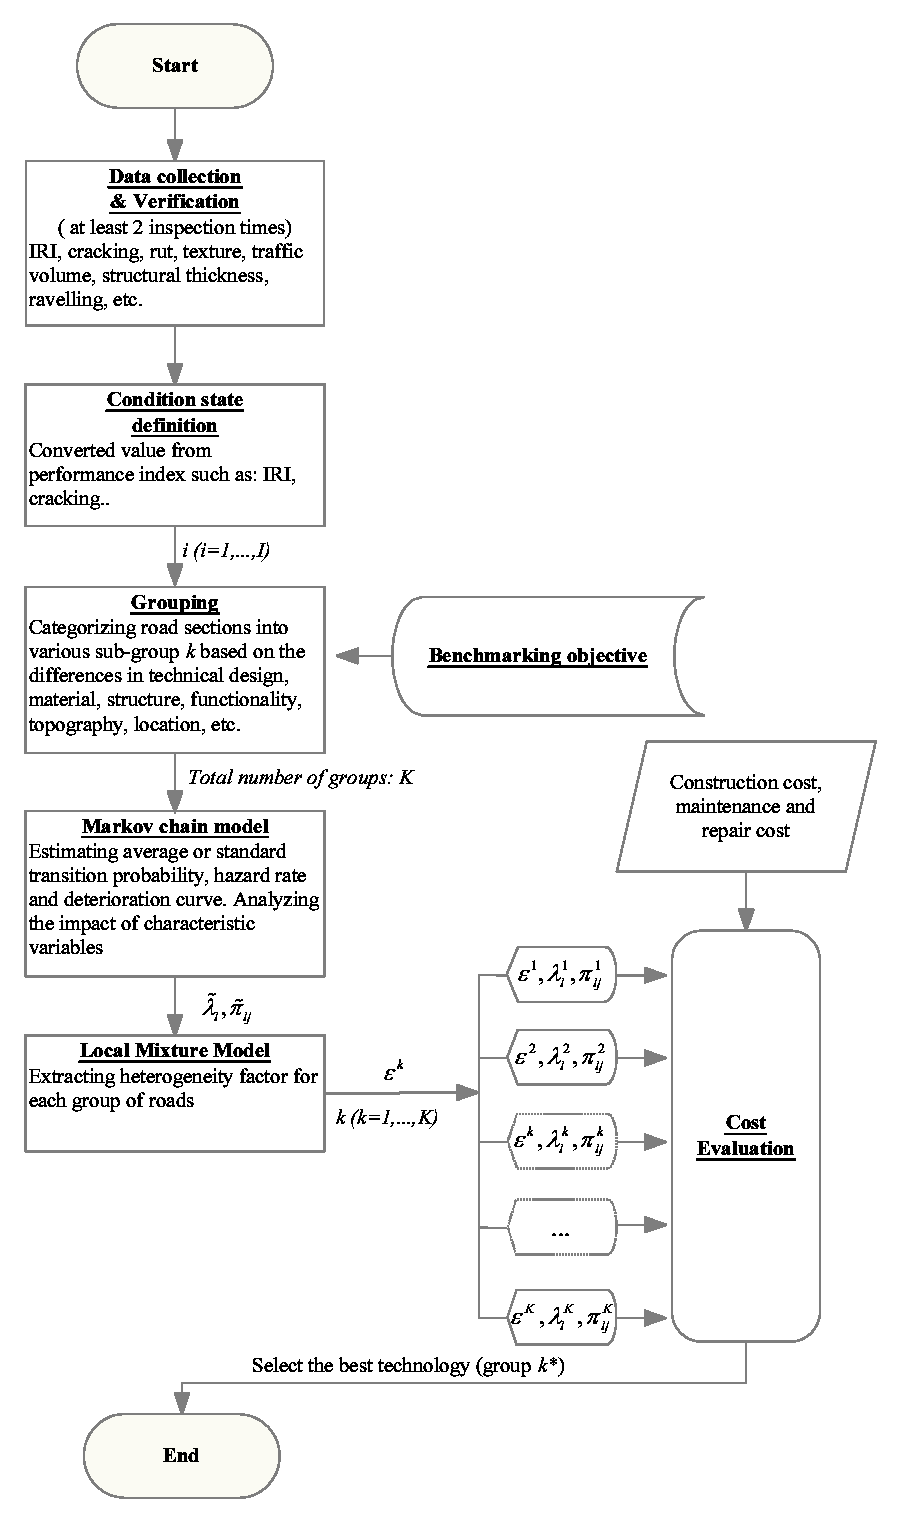
\includegraphics[scale=0.5]{fig62} 
\end{center}
\caption{Benchmarking Flowchart in PMS}
\label{fig62} 
\end{figure}
%%
\section{Empirical study}
\label{66}
\subsection{Overview of empirical study}
\label{661}
In this section, we exploit the applicability of the exponential hazard model to estimate the Markov transition probability. Further, the heterogeneity factor of individual road group is estimated by using the mixture model. Benchmarking study is highlighted with the comparison of deterioration curves. Empirical application is conducted on the monitoring data of the national road system in Vietnam. There are over $10,000$ samples in the database. Each sample represents a road section of 1 km in length. After verification, a sampling population during the period from $2001$ to $2004$ with $6510$ road sections is selected for the empirical test. Information of monitoring data includes the values of indexes such as: International Roughness Index (IRI), Cracking, Texture depth, Thickness of top asphalt layer, Annual traffic volume, etc. The locations of examined road sections are mapped in Figure \ref{fig63}.

In benchmarking study, we consider the deterioration of top surface layers characterizing by type of materials, technical specification, and regional differences. Whilst, the traffic volume and texture depth are considered as characteristic variables. A main reason of the selection is because of having a wide range of choices in the practices of design, construction, and maintenance in Vietnam. In other words, most of pavement technologies are borrowed technologies from developed nations, causing a pavement system of inhomogeneous conditions. The problem of having inhomogeneous conditions in the national pavement system consequently results in a negative influence on maintenance, repair, and renovation. The problem has been documented as a major difficulty for budget allocation either in short or long term strategy.

The original set of monitoring data is filtered and verified in order to define an appropriate range of condition states. Verification 
is necessary since the range of condition states can be converted in various domains from the value of distress. In fact, the values of distress such as Roughness, Cracking, Flatness, and Rut are measured and recorded in a very small scale. Thus, the requirement for defining the range is extremely important. Based on the results of data verification, we realize that the arrival time to the worst condition state are in similar behaviors if different range of condition states are assumed. Hence, for the convenience of observation and computation, we select the range of condition states from $1$ to $5$ as detailed described in Table \ref{table61}. The range of condition states is converted values from the value of IRI.  

\begin{figure}[t]
\begin{center}
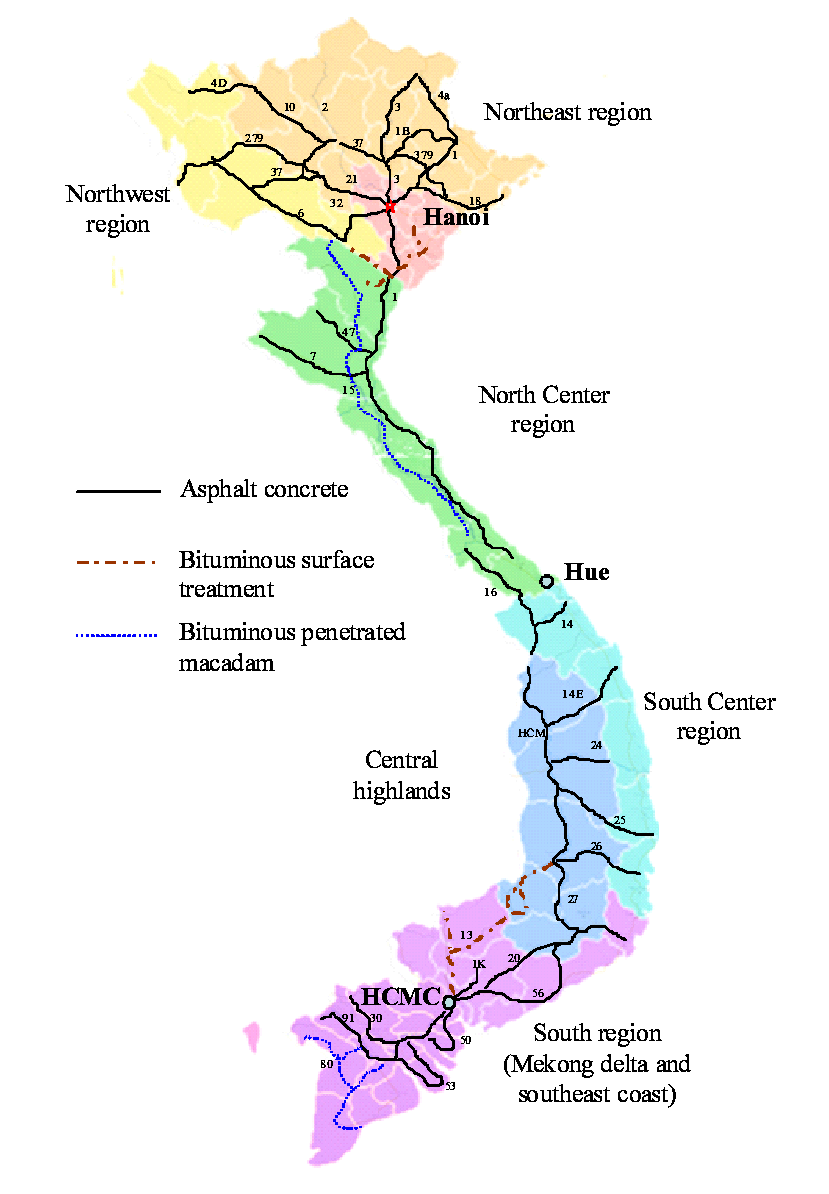
\includegraphics[scale=0.6]{fig63}
\end{center}
\footnotesize Note)  Numbers on the map are the names of national roads.
\caption{Locations of Roads.}
\label{fig63}
\end{figure}

%%%
\begin{table}[t]
\caption{Description of Condition States.}
\label{table61}
{\small
\begin{center}
\begin{tabular}{c|c|c}\hline
Condition states & Range of IRI values & Remark\\\hline
1 & (1-2] & Very good\\
2 & (2-4] & Good \\
3 & (4-6] & Fair \\
4 & (6-8] & Poor \\
5 & $>$ 8 & Very poor \\\hline
\end{tabular}
\end{center}
}
\footnotesize Note) IRI is measured in (m/km).
\end{table}%[t]
\subsection{Estimation results}
\label{662}

In the empirical study, we consider the annual traffic volume of motorized car and the change of texture index as characteristic variables, with denotations as $x_{i2}$ and $x_{i3}$. While, the first characteristic variable $x_{i1}$ equals to 1 as a constant value. The thickness of pavement is not considered in the estimation because it shares a similar range of value in design practices.

Estimation results using the exponential Markov model are displayed in Table \ref{table62}. It is highlighted from the table that the traffic volume has a great influence on the transition of condition state $4$. A strong correlation between the transition of the first two condition states $(i=1,2)$ and the texture depth is also realized. As a matter of fact, the change in the texture depth of road depends on the traffic volume and other environmental conditions such as climate and construction materials. The figures displayed in the parenthesis represent the statistical $t-test$ for the values of unknown parameters.

\begin{table}[t]
\begin{center}
\caption{Estimation Results of Exponential Hazard Model.}
\label{table62}
{\small
\begin{tabular}{c|c|c|c}\hline
Condition & Constant&Traffic volume &Texture depth\\
 states & $\beta_{i1}$ & $\beta_{i2}$& $\beta_{i3}$\\ \hline
1 & 0.7987  &  - &  - \\
& (46.633) & -  &  -\\\hline
2 & 0.004 &  -  &  1.9633 \\\
& (0.547) &  - &  (21.042)\\\hline
3 & 0.225  &  - &  -\\
& (29.629) & - &  -\\\hline
4 & 0.0849 &  3.0108 &  -\\
& (5.8440) &(5.9501)&  -\\\hline
\end{tabular}
}
\end{center}
\footnotesize Note) $t-$ values are shown in the parenthesis.
\end{table}

Eventually, we obtain the values of hazard rate and life expectancy for condition state $i$ through equations (\ref{hazard1}) and (\ref{17}). Results are presented in Table \ref{table63}. It is highlighted that, in average, the life expectancy of condition state $i=1$ lasts less than $1.5$ years before entering into condition state $i=2$. Condition states $2$ has its service life about $5.5$ years. After entering condition state $i=3$, the speed of deterioration accelerates in a fast manner. For instance, condition state $3$ remains only about $4.5$ years before falling to condition state $i=4$. And further, it takes less than $3.5$ years for condition state $i=4$ arriving to the absorbing condition state $(i=5)$.

\begin{table}[t]
\caption{Life Expectancy of Condition States.}
\label{table63}
\begin{center}
{\small
\begin{tabular}{c|cc}\hline
   Condition states& ~$E[\theta_{i}]$~& $E[RMD_{i}^k]$(years) \\\hline
  1 & ~0.7987~ & ~1.2521  \\
   2 & ~0.1835~ & ~5.4488  \\
   3 & ~0.2252~ & ~4.4401 \\
   4 & ~0.2901~ & ~3.4474 \\
   \hline
\end{tabular}
}
\end{center}
\footnotesize Note) The values of hazard rate and life expectancy are not defined for the  absorbing condition state ($i=5$) in Markov chain model.
\end{table}

\begin{table}[t]
\caption{Markov Transition Probability.}
\label{table64}
\begin{center}
{\small
\begin{tabular}{l|lllll}
\hline
\multicolumn{1}{c|}{Condition} & \multicolumn{5}{c}{Condition states} \\ 
\multicolumn{1}{c|}{states} & \multicolumn{1}{c}{1} & \multicolumn{1}{c}{2} & \multicolumn{1}{c}{3} & \multicolumn{1}{c}{4} & \multicolumn{1}{c}{5} \\ 
\hline
\multicolumn{1}{c|}{1} & \multicolumn{1}{c}{0.4499} & \multicolumn{1}{c}{0.4965} & \multicolumn{1}{c}{0.0495} & \multicolumn{1}{c}{0.0038} & \multicolumn{1}{c}{0.0003} \\ 
\multicolumn{1}{c|}{2} & \multicolumn{1}{c}{0.0} & \multicolumn{1}{c}{0.8323} & \multicolumn{1}{c}{0.1496} & \multicolumn{1}{c}{0.0164} & \multicolumn{1}{c}{0.0017} \\ 
\multicolumn{1}{c|}{3} & \multicolumn{1}{c}{0.0} & \multicolumn{1}{c}{0.0} & \multicolumn{1}{c}{0.7983} & \multicolumn{1}{c}{0.1741} & \multicolumn{1}{c}{0.0276} \\ 
\multicolumn{1}{c|}{4} & \multicolumn{1}{c}{0.0} & \multicolumn{1}{c}{0.0} & \multicolumn{1}{c}{0.0} & \multicolumn{1}{c}{0.7482} & \multicolumn{1}{c}{0.2518} \\ 
\multicolumn{1}{c|}{5} & \multicolumn{1}{c}{0.0} & \multicolumn{1}{c}{0.0} & \multicolumn{1}{c}{0.0} & \multicolumn{1}{c}{0.0} & \multicolumn{1}{c}{1.0} \\ 
\hline
\end{tabular}
}
\end{center}
\footnotesize Note) The values of hazard rate and life expectancy are not defined for the  absorbing condition state ($i=5$) in Markov chain model.
\end{table}

\begin{figure}[t]
\begin{center}
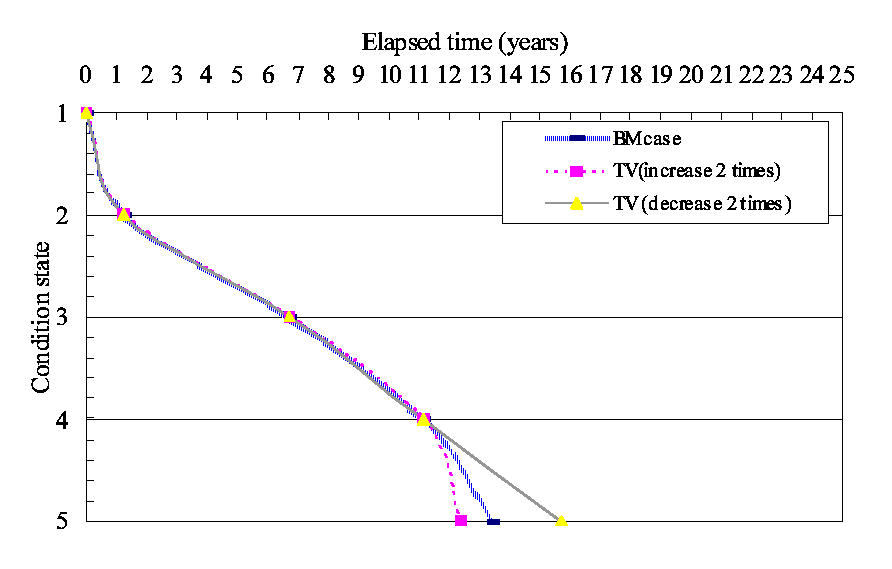
\includegraphics[scale=0.55]{fig64}
\end{center}
\caption{Deterioration Curve.}
\label{fig64}
\end{figure}

The matrix of Markov transition probability, estimated by using the exponential Markov model, is displayed in Table \ref{table64}. The values of transition properties are estimated based on the value of average hazard rate, which represents the deterioration transition pattern of the entire road sections. In order to compare the influence of traffic volume on the deterioration, we carry out the estimations for three cases. The benchmark (BM) case refers to the case that we estimated the hazard rates and transition probability based on annual traffic volume. Whilst, other two cases consider the increase and decrease of annual traffic volume at the rate $0.5$. Comparative results of three cases are illustrated in Figure \ref{fig64}.

An appealing conclusion from Figure \ref{fig63} is that the traffic volume particularly exerts to have a high impact on condition state $4$. In fact, it is true to accept that the traffic volume should affect all the condition states with different severe levels. However, in order to understand its behavior precisely, a richer database of monitoring data is required. Despite the limitation of monitoring data, we are still able to give an alarming message that the deterioration of the road network in Vietnam is progressing with a high speed of deterioration. The life expectancy of the surface layer in the network is relatively less than $13$ years. Probabilistically, after about $6$ years from construction time, the serviceability of the road network cannot satisfy the expectation of users. Thus, it is strongly recommended that Vietnamese road administration should proposes an extensive investigation to find out the causes of high deterioration speed, and works out a suitable plan to prolong the service life of the entire road network.
%%%%%%%%%%%%
\subsubsection{Heterogeneity distribution and deterioration curves}
\label{6621}

\begin{table}[t]
\begin{center}
\caption{Grouping Classification of Roads.}
\label{table65}
{\footnotesize
\begin{tabular}{c|l|c|c|c|c}\hline
   Group& Description & Technical & Speed & Road & Functional  \\
      k  &   & class & flow & class & class \\\hline
   1 & ~Bituminous penetrated macadam~(226) & ~60 & 3+4 & 1 & 3   \\
   2 & ~Bituminous surface treatment~(1301) & ~60 & 1+3+4 & 1+2 & 3+4+5   \\
   3.1 & ~Asphalt concrete ~(713) & ~40 & 4 & 1 & 4   \\
   3.2 & ~Asphalt concrete ~(1047) & ~60 & 3 & 2 & 2  \\
   3.3 & ~Asphalt concrete ~(1030) & ~60 & 3 & 1 & 3  \\
   3.4 & ~Asphalt concrete ~(467) & ~60 & 3 & 1 & 4  \\
   3.5 & ~Asphalt concrete ~(602) & ~60 & 3 & 2 & 3    \\
   3.6 & ~Asphalt concrete ~(1025) & ~80 & 3 & 1 & 2   \\
   3.7 & ~Asphalt concrete (99)~ & ~60 & 4 & 1 & 3  \\
  \hline
\end{tabular}
}
\end{center}
\footnotesize Note) Figures in the parenthesis shows number of data. Technical class is defined by maximum allowance speed used in design. Speed flow is categorized in the range (\textbf{1}-single lane with width $<=$3.5m; \textbf{2}-3 lanes with width of 10-14.5 m; \textbf{3}-2 lanes with width of 3.5-5.5 m; \textbf{4}-2 lanes with width of 5.5-10.5m; \textbf{5}- 4 lanes with width $>=$ 14m). Road class \textbf{1} refers to main tracks of national roads, \textbf{2} is supplement tracks of national roads. Functional class refers to management level \cite{tcvn4054}. Group 1 and 2 are classified with a combination of several designated factor.
\end{table}

In the benchmarking study, we categorize $6510$ road sections into three groups according to the types of materials. In addition, we further classify the group of asphalt concrete materials into seven smaller groups based on the technical class, speed flow, road class, and functional class since this group accounts for a large number of samples in monitoring data. Thus, the total number of groups are nine, with the detailed description explained in Table \ref{table65}. The locations of roads belonging to each group are also highlighted in Figure \ref{fig62}. Estimation results for heterogeneity factor of individual group by employing both parametric and semi-parametric approaches are also given in Figure \ref{fig64} and Figure \ref{fig65}. 

\begin{figure}[t]
\begin{center}
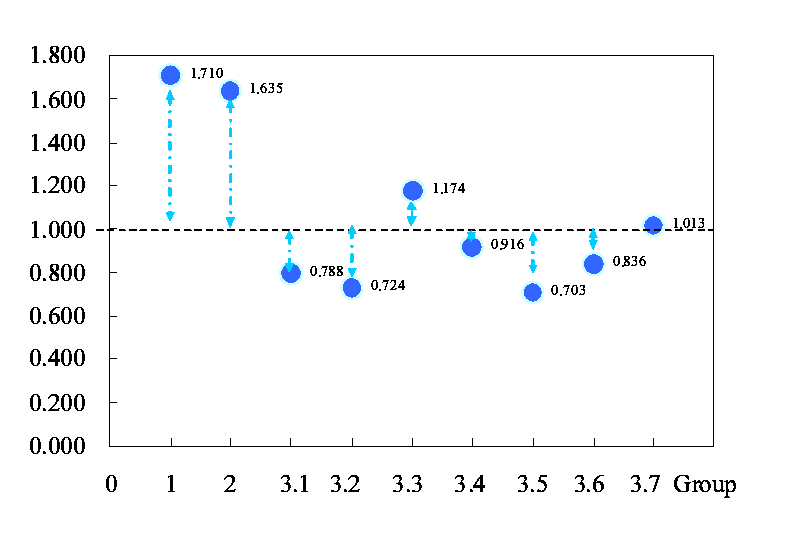
\includegraphics[scale=0.5]{fig65}
\end{center}
\caption{Distribution of Heterogeneity Factors - Parametric Approach.}
\label{fig65}
\end{figure}

\begin{figure}[t]
\begin{center}
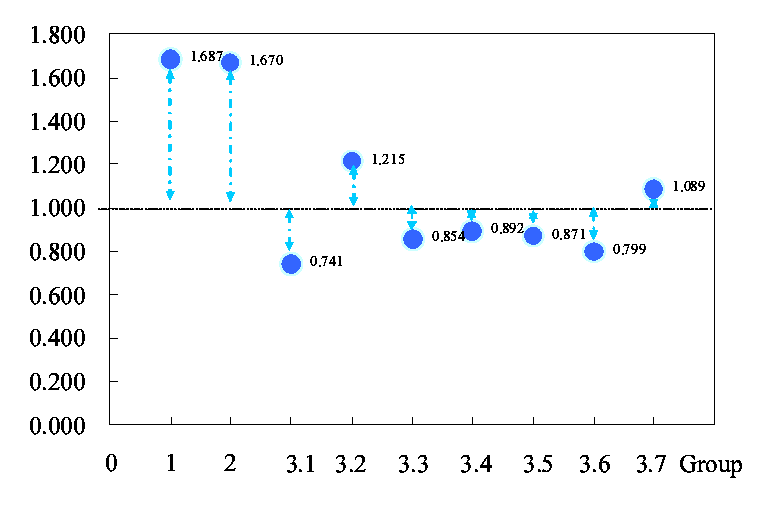
\includegraphics[scale=0.5]{fig66}
\end{center}
\caption{Distribution of Heterogeneity Factors - Semi-parametric Approach).}
\label{fig66}
\end{figure}

Comparisons of deterioration curves are drawn in Figure \ref{fig67} with parametric approach and in Figure \ref{fig68} with semi-parametric approach. The figures shows the deterioration curves of roads based on $3$ types of materials. The group of roads with asphalt overlays has a longest service life (about 16 years). Meanwhile, the two other groups of roads with materials composing of bituminous penetrated macadam and bituminous surface treatment have their service life less than $9$ years. Since asphalt concrete becomes a popular material for overlay, most of national roads are now paved with asphalt concrete. Thus, we further classified the group of asphalt concrete into $7$ sub-groups and compared their deterioration curves. In total, there are nine groups of roads for benchmarking. Figure \ref{fig69} and Figre \ref{fig610} presents the a comparative view on the deterioration curves of $9$ groups. It is realized that deterioration curves of asphalt concrete surfaces has a small dispersion in compare with other groups. Relatively, the life expectancy of asphalt concrete surfaces ranges from $12$ to $16$ years.

\begin{figure}[t]
\begin{center}
\includegraphics[scale=0.5]{fig67}
\end{center}
\caption{Deterioration Curves - 3 Types of Road Materials - Parametric approach.}
\label{fig67}
\end{figure}

\begin{figure}[t]
\begin{center}
\includegraphics[scale=0.5]{fig68}
\end{center}
\caption{Deterioration Curves - 3 Types of Road Materials - Semi-parametric Approach.}
\label{fig68}
\end{figure}
%
%
\begin{figure}[t]
\begin{center}
\includegraphics[scale=0.5]{fig69}
\end{center}
\caption{Deterioration Curves-9 Groups - Parametric Approach.}
\label{fig69}
\end{figure}

\begin{figure}[t]
\begin{center}
\includegraphics[scale=0.5]{fig610}
\end{center}
\caption{Deterioration Curves-9 Groups - Semi-parametric Approach).}
\label{fig610}
\end{figure}
\begin{figure}[t]
\begin{center}
\includegraphics[scale=0.5]{fig611}
\end{center}
\caption{Deterioration Curves-regional Perspective (6 regions) - Parametric  Approach.}
\label{fig611}
\end{figure}
%%
\begin{figure}[t]
\begin{center}
\includegraphics[scale=0.5]{fig612}
\end{center}
\caption{Deterioration curves-Deterioration Curves - Regional Perspective (6 regions) - Semi-parametric Approach.}
\label{fig612}
\end{figure}

According to the climate zones of Vietnam, road sections with asphalt concrete overlay are classified into $6$ regions. The location of each region is also displayed in the map of Figure \ref{fig63}. A comparative view of the deterioration curves of asphalt roads according to regional classification are illustrated in Figure \ref{fig611} and Figure \ref{fig612}. As can be seen from two figures, it is proved that the deterioration of road surfaces in the southern part is faster than that of road surfaces in the northern regions. This reason could possibly due to the effects of soft ground condition in the southern part of Vietnam or the impact of flooding in low land areas. The two prominent reasons are strongly believed to cause the subsidence of construction works in the southern part of the country. The deterioration of road surfaces in the north part of the country has a slower speed than the that of the other regions. Moreover, it is also found that that deterioration speed of road surfaces in urban areas is faster than that in the highland regions. The faster deterioration speed in the urban areas is due to the effects of heavier traffic volume annually.

Throughout the analysis and comparison of estimation results as presented in the above figures, it is realized that the there exists variations of estimation results between two methodologies (Parametric and Semi-parametric). However, the variations are observed in a small scale. Thus, the two approaches can be supplementary used for each other in order to improve the quality of estimation.
%
%%%
\subsubsection{Cost Evaluation}
\label{6622}
In view of economic evaluation, a simple cost evaluation technique is applied. We assumed that whenever the condition state of a road section reaching the absorbing state $(i=5)$, renewal will be implemented. The total cost is a summation of construction cost and renewal cost for renewing the overlay. With this assumption, the average cost of construction and renewal for each type of road surface according to its material can be estimated, simply by calculating the ratio of its total cost to its average life expectancy. 

The results of cost estimation are presented in Table \ref{table66}. The results highlight the fact that higher benefit can be earned if the asphalt concrete overlay is applied instead of applying the bituminous penetrated macadam and bituminous surface treatment overlays. A significant difference in the life expectancy and average cost within the group of asphalt concrete material is also realized from the estimation results in Table 6. Based on the obtained results, the best type of overlay for long term application can be recommended. For example, group 3.1 in Table \ref{table66} is considered as the best one in term of economic perspective. 

\begin{table}%[t]
\begin{center}
\caption{Average Cost Evaluation.}
\label{table66}
{\small
\begin{tabular}{c|c|c|c}\hline
   Group&  Renewal & Service & Average \\
      k  & cost  & life (years)  & cost \\\hline
   1 &  ~8,567 & 7.64   & 1,121 \\
   2 &  ~8,929 & 7.72    & 1,157 \\
   3.1 &  ~11,754 & 17.38   & 676 \\
   3.2 &  ~11,754 & 10.61   & 1,108 \\
   3.3 &  ~11,754 & 15.09  & 779 \\
   3.4 &  ~11,754 & 14.45   & 814 \\
   3.5 &  ~11,754 & 14.79   & 795 \\
   3.6 &  ~11,754 & 16.12   & 729 \\
   3.7 &  ~11,754 & 11.84   & 993 \\
   \hline
\end{tabular}
}
\end{center}
{\small Note) Monetary unit is $1000$ thousand Vietnamese dong. Unit cost is referred to the standard norm cost defined by Hanoi construction bureau \cite{dghanoi08,dm1242}. Cost is estimated for 100 $m^2$ and 5 cm in its thickness of road.}
\end{table}
%
%
% Deterioration curve with respect to each hetegoneity factor 
\section{Summary and Recommendations}
\label{67}
This chapter has proposed a mixture model for benchmarking study. The mixture model is expressed by means of heterogeneity factor $\epsilon$ that exists in each group of roads. The heterogeneity factor is considered to follow the Gamma distribution (Parametric approach) and the function of Taylor series (Semi-parametric approach). In order to estimate the heterogeneity factor, two steps estimation approach with maximum likelihood estimation method is applied. The mixture hazard model is considered as an excellent tool for benchmarking study, which is used to search for the best technology in the pavement management system. In view of practical application, the methodology is suitable to apply in the pavement management system of developing countries like Vietnam, where has a high demand of standardization in the pavement system.

To demonstrate the applicability of the model, we conducted an empirical study on a database of Vietnamese pavement system collected during the years $2001$ and $2004$. The technological groups were classified according to the types of materials and regional zones. The estimation results revealed a fact that the speed of deterioration of roads in Vietnam is very fast. Approximately $10$ years after construction, the condition states of road surfaces reach the worst condition state. The main cause leading to the fast deterioration is because of the high intensity of annual traffic volume. Furthermore, estimation results prove that the performances of road surfaces with asphalt concrete are much better than that of the road surfaces with bituminous penetrated macadam and bituminous surface treatment. Based on a simple cost evaluation technique, the empirical study also recommended a best group of road surfaces with asphalt concrete for long term application. 

However, we have not discussed several points, which will be considered as topics for extending this study in the future:

\begin{itemize}
\item The benchmarking study focused only on the pavement management system. However, its application can be applied to other types of infrastructure.
\item This chapter proposed only a simple cost evaluation technique, which does not considered the routine maintenance and repair actions. In order to overcome this limitation, a cost evaluation technique using the theory of Markov decision process should be applied in the future extension of the model.
\item This chapter has not discussed the problem of measurement errors in monitoring data, which is one of the main reason causing the bias in estimation results. A future study shall consider the theory of hidden Markov models, Bayesian estimation, and Markov Chain Monte Carlo into account.
\item The empirical study of this chapter just focused on a small scale application of benchmarking methodology on the pavement system in Vietnam, particularly focusing on the types of materials and regional zones. However, in order to find out the best pavement technology and to propose a feasible solution to the problems of pavement system in Vietnam, a better quality monitoring data shall be accumulated.
\item In the empirical study, we considered only the annual traffic volume as a time-invariant characteristic variable. However, in reality, the intensity of annual traffic volume is always dynamic and change with time. Therefore, it is recommended that future extension of the study shall consider the traffic volume as a time-variant characteristic variable.
\end{itemize} % Benchmarking and mixture model

\input{./Chapters/Chapter7} % Conclusion
%% ----------------------------------------------------------------
% Now begin the Appendices, including them as separate files

\addtocontents{toc}{\vspace{2em}} % Add a gap in the Contents, for aesthetics

\appendix % Cue to tell LaTeX that the following 'chapters' are Appendices
% Appendix A

\chapter{Appendix A}
\lhead{Appendix A. \emph{Estimation Method for LCC}}
\label{Appendix A}
Solution to Gamma function in the equation of life cycle cost $J(0,z)$
\begin{eqnarray}
&& J(0:z)= \frac{(c+I)\Gamma(z)+I \Lambda(z)}{1-\Gamma(z)-\Lambda(z)} \label{a1}
\end{eqnarray}
Where $\Gamma(z)$ and $\Lambda(z)$ functions are defined as follow (without considering the risk factor since it is not of neccessity to represent for general calculation):
\begin{eqnarray}
&& \Gamma(z)=\int_0^{z} f(t)\exp(-\rho t)dt \nonumber \\
&& \hspace{5mm}= \int_0^z \alpha m\tau^{m-1}\exp(-\alpha \tau^m-\rho t)dt \label{gamma1}\\
&& \Lambda(z)= \tilde{F}(z) \exp(-\rho z)  \nonumber \\
&& \hspace{5mm} =\exp(-\alpha z^m-\rho z)  \label{alpha1}
\end{eqnarray}
Gamma function in equation (\ref{gamma1}) can be extended in the following way
\begin{eqnarray}
\Gamma(z)= \int_0^z (\alpha m\tau^{m-1}+\rho-\rho)\exp(-\alpha \tau^m-\rho t)dt \label{gamma11}\\
 \Leftrightarrow  - \int\limits_0^z {\exp ( - \alpha t^m  - \rho t)d( - \alpha t^m  - \rho t)}\nonumber \\ 
- \rho \int\limits_0^z {\exp ( - \alpha t^m  - \rho t)dt}\nonumber  \\ 
 = 1 - \Lambda (z) - \rho \int\limits_0^Z {\exp ( - \alpha t^m  - \rho t)dt} \label{gamma2}
\end{eqnarray}
The denominator in equation (\ref{a1}) becomes
\begin{eqnarray}
1 - \Lambda (z) - \Gamma (z) = \rho \int\limits_0^z {\exp ( - \alpha t^m  - \rho t)dt} \label{deno} 
\end{eqnarray}
Subtitute equations (\ref{gamma2}) and (\ref{deno}) into (\ref{a1}), following results are obtained
\begin{eqnarray}
J(0,z) = \frac{{(C + I)\left[ {\Gamma (z) + \Lambda (z) - 1} \right] + C + I - C\Lambda (z)}}{{1 - \Lambda (z) - \Gamma (z)}} \label{a2}\\
=\frac{{C + I - C\Lambda (z)}}{{\rho \int\limits_0^z {\Lambda (t)dt} }} - (C + I) \label{a3}
\end{eqnarray}
Here, we have to solve the integration of function $\Lambda (z)$. The general form of expanding the integration into following discrete series will be accepted.
\begin{eqnarray}
I_k  = \int\limits_0^{kdt} {f(x)dx} 
\end{eqnarray}
Here, $k$ is number of iteration and $dt$ is the very small amount of time. For example, value of $d$ can becomes $d=0.01$ or $0.001$ or even smaller. 
\begin{eqnarray}
I_{k + 1}  = \int\limits_0^{(k + 1)dt} {f(x)dx} \\
=I_k  + \int\limits_{k.dt}^{(k + 1)dt} {f(x)dx} \\
= I_k  + \frac{{[f(kdt) + f\{ (k + 1)dt\} ]dt}}{2} \label{i1}
\end{eqnarray}
To this point, the value of integration can be easily estimated by numerical calculation. We subtitute equation (\ref{a3}) and use Newton method to estimate for the minimum value of $J(0,Z)$ with respect to the increasing number of year $Z$.

Beside this method, the Simpson rule for solving integration can also be applied. However, a comparison with various small values of $d$ proves that the above method is sufficient enough in satisfying the objective of chapter \ref{Chapter5}.

%First derivative of likelihood function with respect to $\alpha$ and $m$
%\begin{eqnarray}
%\frac{{\partial \ln \ell (\alpha ,m:t_s )}}{{\partial \alpha }} = \sum\limits_s^S {\left[ {(1 - \delta _s )( - t_s^m ) + \delta _s \left\{ {\frac{1}{\alpha } - t_s^m } \right\}} \right]}  = \sum\limits_s^S {\delta _s \frac{1}{\alpha } - t_s^m } 
%\end{eqnarray}
%\begin{eqnarray}
%\begin{array}{l}
%\frac{{\partial \ln \ell (\alpha ,m:t_s )}}{{\partial m}} = \sum\limits_s^S {\left[ {(1 - \delta _s )( - mt_s^{m - 1} ) + \delta _s \left\{ {\frac{1}{m} + \ln t_s  - \alpha mt_s^{m - 1} } \right\}} \right]}  \\ 
%  = \sum\limits_s^S {\frac{{\delta _s }}{m} + \delta _s \ln t_s  - \alpha mt_s^{m - 1} }  \\ 
% \end{array}
%\end{eqnarray}

%First derivative of likelihood function with respect to $\alpha$ and $m$
%\begin{eqnarray}
%&&\frac{{\partial \ln \ell (\alpha ,m:t_s )}}{{\partial \alpha \partial \alpha }} = \sum\limits_s^S { - \delta _s \frac{1}{{\alpha ^2 }}} 
%\\
%&&\frac{{\partial \ln \ell (\alpha ,m:t_s )}}{{\partial \alpha \partial m}} = \frac{{\partial \ln \ell (\alpha ,m:t_s )}}{{\partial m\partial \alpha }} = \sum\limits_s^S { - mt_s^{m - 1} } 
%\\
%&&\frac{{\partial \ln \ell (\alpha ,m:t_s )}}{{\partial m\partial m}} = \sum\limits_s^S {\left[ { - \alpha \left\{ {t^{m - 1}  + m(m - 1)t^{m - 1} } \right\} - \frac{{\delta _s }}{{m^2 }}} \right]} 
%\end{eqnarray}	% Appendix Title

%\input{./Appendices/AppendixB} % Appendix Title

%\input{./Appendices/AppendixC} % Appendix Title

\addtocontents{toc}{\vspace{2em}}  % Add a gap in the Contents, for aesthetics
\backmatter

%% ----------------------------------------------------------------
\label{Bibliography}
\lhead{\emph{Bibliography}}  % Change the left side page header to "Bibliography"
\bibliographystyle{unsrtnat}  % Use the "unsrtnat" BibTeX style for formatting the Bibliography
\bibliography{Bibliography}  % The references (bibliography) information are stored in the file named "Bibliography.bib"
\newpage
\lhead{\emph{Contact Information}} 

Le Thanh Nam\\
Email address: namkyodai@gmail.com\\
%Url:	http://namlt.blogspot.com\\

\textit{Home address in Vietnam:}\\
Vien Nghien Cuu Nuoi Trong Thuy San I\\
Dinh Bang - Tu Son - Bac Ninh - Vietnam\\
Tel: +84-(0)4 3878 0100
\end{document}  % The End
%% ----------------------------------------------------------------